\documentclass[a4paper,11pt,titlepage]{article}
\usepackage[margin=3cm]{geometry}
\usepackage{hyperref}
\usepackage[nodayofweek]{datetime}
\longdate
%landscape
\usepackage{lscape}
\usepackage{pdflscape}
\usepackage{amssymb}
\usepackage{placeins} %Floatbarrier
\usepackage{graphicx}
\usepackage{enumitem}
\usepackage{fancyhdr}
\usepackage{bbm}
\usepackage{amsmath} %matrices
%Tables
\usepackage[table,xcdraw]{xcolor}
\usepackage[normalem]{ulem}
\useunder{\uline}{\ul}{}
%for pseudo code
\usepackage{algorithm}
\usepackage[noend]{algpseudocode}
%for label matrix
\usepackage{amsmath}
\usepackage{bm}
\usepackage{stackengine}
\usepackage{mathtools}
% Please add the following required packages to your document preamble:
\usepackage[normalem]{ulem}
\useunder{\uline}{\ul}{}
%Frames
\usepackage{framed}
\usepackage{caption}
\usepackage{cite}
%longtable
\usepackage{longtable}

\usepackage{biblatex}
\addbibresource{references.bib}

\pagestyle{fancyplain}
\fancyhf{}
\lhead{\fancyplain{}{MSc Individual Project}}
\rhead{\fancyplain{}{\today}}
\cfoot{\fancyplain{}{\thepage}}
\setlength{\headheight}{14pt}
\setlength\parindent{0pt}

\title{Machine Learning on Stochastic Networks\\\Large{--- Individual Project Final Report---}}
\author{Alfred Tingey\\
       aft19@imperial.ac.uk\\ \\
       \small{Supervisor: Giuliano Casale}\\
       \small{Imperial College London} 
}

\begin{document}
\maketitle

\large
\begin{center}
\textbf{Abstract} \\
\end{center}
In this paper we will analyse how to use multiple machine learning algorithms to infer the characteristics and behaviour of stochastic processes from observed data. We focus on applying most of our algorithms to a special sub-section of stochastic processes called queueing networks.  Our main body of work explores 3 areas of machine learning that can be applied to stochastic processes: Expectation-Maximization algorithms, Markov-Chain Monte Carlo methods and recurrent neural networks. We aim to use the EM algorithm to predict parameters of Markov Arrival Processes from traces of inter-arrival rates; a Gibbs sampling MCMC method to estimate the demands of certain queueing networks from the steady state average queue lengths of the system; and a recurrent neural network to predict the parameters of queueing networks from an input trace of the average queue lengths of the system over time. The aim of this project is to evaluate the suitability of each method to be able to accurately predict parameters of the system that created the data. In our evaluation, we compare the accuracy of our algorithms over various network models and how well they generalize to the networks. \\

Most of our software implementation works directly with the MATLAB toolbox LINE [LIN20]. We can build, analyse and predict aspects of queueing networks using this toolbox. Part of our project aim is to create machine learning methods using MATLAB such that we can extend LINE with our implementation of the methodology. 

\clearpage

\large
\begin{center}
\textbf{Acknowledgements} \\
\end{center}

The following list details the people that I would like to thank for helping me complete this project:

\begin{enumerate}
    \item Firstly, I would like to thank my supervisor, Giuliano Casale. He has offered me unwavering support throughout this process; he was prompt in answering any questions I may have had; and he helped guide me through the numerous difficulties that arose in this project. 
    \item Secondly, I would like to thank Mark Van der Wilk for offering me feedback on my background and progress report. 
    \item Thirdly, I would like to thank my flatmates Roberto, Jack and Salva for spurring me on over the last 3 months. Due to COVID and lock-down, I spent a significant amount of time with them whilst in the midst of this project, and they valiantly helped push me towards its completion.
    \item Lastly, I would like to thank my parents for always supporting me.
\end{enumerate}

\clearpage

\tableofcontents

\clearpage

\section{Introduction}

\subsection{Motivation}

To understand the motivation for this project, we must first understand the external importance of queueing networks. Queueing theory has great significance as a research area because of its huge and relevant applications across industry [Kin84], [Cas16], [Kaw17], [Bol06], [Gei82]. A queueing network can be built from anything that has customers and servers: the customers get served through a certain service discipline and the excess customers must wait in a queue to be served. The simplest example of a queueing network would be akin to waiting in line at a petrol station, where there is one person working at the petrol station serving each customer one at a time in a first-come first served discipline. However, we could also create queues that have bewildering complexity and are much harder to imagine. \\

It is simple to imagine the benefits of understanding queueing theory when applied to a certain industry. Queueing theory can help create more efficient develop pricing mechanisms, staffing solutions, arrival management strategies, placement of servers, and many more fundamentally important aspects of real applications within industry. As an example, imagine queueing theory applied to a hospital. We can use queueing models to estimate the waiting time for a specific patient [Ahm17]; analyse customer satisfaction [Nos01]; develop an efficient scheduling template of a chemotherapy treatment unit [Ahm11]; and maximize the utility of each service system [Bah17]. This is not unique to hospitals, and can be applied to many industrial sectors, such as: banks [Xia10], ATMs [Pat12], port equipment sizing [Dra17], traffic systems [Buc03], and electric vehicle charging stations [Zha16]. \\

The applications of queueing theory do not stop here. One can also use queueing theory to analyze computer systems [Gie82], blockchain mechanisms [Kaw17], communication networks [Kin84] and web services [Cas16]. For example, the ability to deliver guaranteed quality of service is fundamental for the success of cloud platforms. Furthermore, performance modelling of web applications requires an understanding of estimating service demands of requests at physical resources, such as CPUs [Cas13].\\

The wide application and significance of queueing theory fuels our motivation for this topic. In this project, we aim to build machine learning tools to predict parameters of queueing networks and Markov Arrival Processes, which in practice can be applied to real industrial data. 

\subsection{Aims}

The overarching aim of our project is to identify, theorize and implement various machine learning algorithms that can be used on stochastic processes. In order to accomplish this goal, we firstly describe the mathematical theory of stochastic processes and queueing networks. We then identify problems that can be solved by using machine learning algorithms. Subsequently, we tackle the theory of each machine learning algorithm and how it works. Finally, for each machine learning algorithm, we implement and evaluate the suitability of the algorithm by using the software MATLAB and with the help of the LINE toolbox. \\

The machine learning algorithms that we build can then, in theory, be used as an extension to the LINE toolbox. In this project we will look in great detail at three machine learning algorithms applied to various stochastic processes: an expectation-maximisation algorithm applied to Markov Arrival Processes; a Markov-Chain Monte Carlo method Gibbs sampling that can be used for demand estimation when applied to certain queueing networks; and a recurrent neural network model that can be used to predict the parameters of the underlying continuous-time Markov Chain when applied to specific queueing networks. The aim of each algorithm is similar: to predict certain behavioural aspects of the stochastic process in question with the highest accuracy possible. In order to do this, we look at many different examples of queueing networks and assess the suitability of our algorithms. 

\subsection{Contributions}

The contributions of this project are based on the machine learning algorithms that we implement. In this section we will describe the structure of this paper and the contributions present in each section. This paper is structured as follows. We firstly introduce background reading topics and the essential knowledge required for comprehension of later ideals in the paper. Then, for each machine learning algorithm, we describe the mathematical theory behind the algorithm; explain how it works; and evaluate the results of our implementation of the algorithm.  \\

In Section 3 we mathematically describe and analyze the fundamental aspects of queueing networks and queueing theory that are required to understand this paper. It is important to include this section for self-containment: one should only need this paper and a solid understanding of mathematics to be able to comprehend everything that we discuss. In Section 4 we introduce our first algorithm: the EM algorithm applied to Markov Arrival Processes. In this section we implement 2 versions of an EM algorithm, a naive version and an improved version. We discuss why the improved EM algorithm is better suited to our problem than the naive algorithm. Section 5 evaluates the results of our improved EM algorithm. Section 6 describes 2 MCMC methods for demand estimation: Gibbs sampling and the Metropolis Hastings algorithm. Section 7 evaluates our results for the Gibbs sampling method. Section 8 describes the mathematics behind our recurrent neural network for parameter estimation using transient averages of queue length data. Section 9 evaluates the results of our RNN implementation and discusses any improvements that can be made to our implementation. \\

We summarize the contributions of this paper as follows: 

\begin{enumerate}
    \item Description of queueing networks as detailed in [Bol06].
    \item Implementation and description of EM algorithm for MAP fitting as detailed in [Buc03].
    \item Implementation and description of EM algorithm for MAP fitting as detailed in [Hor18], [Hor13] and [Oka08].
    \item Application of our EM algorithm to real-world data, with discussion on suitability and evaluation of results. The real data is taken from [ITA].
    \item Implementation and description of MCMC method Gibbs sampling for demand estimation as detailed in [Cas13] and [Cas16].
    \item Description of how to apply Metropolis Hastings algorithm to demand estimation, as detailed in [Cas13]. 
    \item Discussion on how to apply Gibbs sampling when we do not have enough samples, as detailed in [Cas16]. 
    \item Implementation and description of recurrent neural networks for parameter fitting of queueing networks as detailed in [Gar20].
    \item An analysis on how unseen server concurrency values affect the error in our RNN predictions. 
\end{enumerate}

\subsection{Consideration of Ethical Implications within this Project}

In this section we will consider and evaluate the ethical issues and implications of this project. We are in a situation where this project is mainly focused on the mathematical theory of machine learning algorithms applied to stochastic processes. We focus on how suitable these algorithms are for certain examples and their respective successes and failures when predicting parameters of networks and systems. Our machine learning algorithms are used to predict parameters of complex mathematical systems, therefore we do not run into many ethical issues, if any at all. As can be seen by Tables \ref{tab:ethical_checklist1} and \ref{tab:ethical_checklist} in the ethical checklist appendix, we have marked `no' for every ethical complication that has to be considered for this project. This is because we do not require any use of personal data for this project, and nothing that we implement has any ethical problems. Now, this does not mean that this area of research does not have the potential to run into ethical complications, it just means that in this specific project ethical issues have not arisen. \\

For the sake of argument, we will briefly discuss a situation where this project could have ran into ethical issues. Imagine we were to collect real queueing network data from a business, let's say a hospital, and we wanted to use our algorithms to infer parameters of the resulting queueing system. The data that we would require to use our algorithms on are either: the inter-arrival times of jobs in the system; the steady state queue lengths of the system; or the transient queue length of the system over time. In the case of a hospital, these could be respectively represented as: the average time taken for a doctor to service a patient; the average amount of patients waiting to see a doctor in a day at the hospital; and the amount of patients waiting to see a doctor every minute of the day averaged over several days. This hypothetical data that we collect on its own doesn't seem to run into any issues as none of it is personal. However, if we were to imagine that each patient waiting in the queue were not anonymous, then we would be using our algorithms on personal data and ethical implications could arise. For example, if we were to consider how the average queue length changed depending on a person's race or sex then ethical implications could arise. If we were to consider how the queue length changed depending on which department of the hospital we were in then ethical complications could arise, and so on and so forth. \\

This is an interesting topic of discussion because the inference of parameters that we implement in this paper could have ethical implications depending on the type of data that we collect. However, in this project we do not use any personal data. In fact, the only data that we use is totally anonymous and is based on LAN traffic, as explained in [ITA]. As a result of this, we do not have any ethical complications, and we do not need to consider them further. 

\section{A Brief Introduction to Stochastic Processes}

The aim of this project is to optimize and perform inference on stochastic models that describe access to resources, such as networks of queues and caches. Firstly, we will discuss simple stochastic processes such that we are able understand the nuances behind the more complex models that we will delve into further at a later time. The information from this chapter has been summarised from [Bol06], [Gil91], and [Ibe13].\\

A stochastic process is defined as a family of random variables $\{X_t : t \in T\}$ where each random variable $X_t$ is indexed by a parameter $t \in T$. The set of all possible values of $X_t$ is called the state space of the stochastic process, denoted as $S$ [Bol06]. \\

A stochastic process can either be a discrete-parameter process or a continuous-parameter process. If the set $T$ is discretely-parametered and is countable, then the stochastic process is a discrete-parameter process. If the set $T$ is continuously-parametered, or the set is not countable, then the stochastic process is a continuous-parameter process. Additionally, the state space $S$ of a stochastic process can either be continuous or discrete. Continuous-paramater stochastic processes can be probabilistically chategorized by the joint cumulative distribution function $F_X(s;t)$ for a given set of random variables $\{X_{t_1}, X_{t_2}, ..., X_{t_n}\}$, parameter vector $t = (t_1,t_2,...t_n) \in \mathbb{R}^n$ and state space vector $s = (s_1,s_2,...,s_n) \in \mathbb{R}^n:$

\begin{equation}
F_x(s;t) = P(X_{t_1} \leqslant s_1, X_{t_2} \leqslant s_2,...,X_{t_n} \leqslant s_n).    
\end{equation}

Consequently, we can define the probability density function (pdf) using partial derivatives in the following form: 

\begin{equation}
f_x(s;t) = \frac{\partial ^ n F_x(s;t)}{\partial s_1 \partial s_2 ... \partial s_n}
\end{equation}

if the partial derivatives exist. A stochastic process $\{X_t : t \in \mathbb{R}\}$ is the same as a Markov process if the Markov property is satisfied for the stochastic process. The Markov property states that the conditional CDF of $X_t$ only depends on the previous state $X_{t-1}$ for any value of t in the stochastic process. We will now discuss Markov processes in significant detail. 

\subsection{Markov Processes and Markov Chains}

The information and equations present in this section have been summarised from the references [Bol06], [Gil91], [Tol16] and [Ibe13]. Markov Processes provide very `flexible, powerful and efficient means for the description and analysis of dynamic system properties' [Bol06]. As this project has a distinct focus on queueing systems, Markov Processes are crucial to understand as they constitute the fundamental theory underlying that of queueing systems. A stochastic process $\{X_t : t \in \mathbb{R}\}$ is equivalent to a Markov process if: $ \forall t_i: 0 = t_0 < t_1...< t_n < t_{n+1}$ and $ \forall s_i \in S$ the conditional CDF of $X_{t_{n+1}}$ depends only on the previous value $X_{t_{n}}$ and not on the earlier values. Put succinctly into equation form, we have that a stochastic process constitutes a Markov process if: 
\begin{equation}
    P(X_{t_{n+1}} \leqslant s_{n+1} | X_{t_{n}} = s_n,..., X_{t_{1}} = s_1, X_{t_{0}} = s_0) \\
    = P(X_{t_{n+1}} \leqslant s_{n+1} | X_{t_{n}} = s_n)
    \label{eqn:stochastic_to_markov}
\end{equation}

Equation \ref{eqn:stochastic_to_markov} represents the most important aspect of a Markov process: the whole history of a Markov chain is summarised in the current state $X_{t_n}$. We can also word this as follows: given a present state, the future is conditionally independent of the past [Bol06]. We will now follow the assumption that we only consider discrete Markov processes, which we denote as Markov chains. These are Markov processes that are constrained to a discrete, finite or countably infinite state space, $S$, and a discrete-parameter space $T$. We can set $T \subseteq \mathbb{N^+}$ as this terminology is easy to work with [Bol06]. When we work with discrete Markov processes, we use probability mass functions (pmf) instead of probability density functions. We use the conditional pmf reflecting the Markov property for discrete-time Markov chains. A stochastic process is defined as a discrete-time Markov chain if at consecutive points of observation the following relation on the conditional pmf holds for all $n \in \mathbb{N}_0$ and all $s_i \in S$: 

\begin{equation}
P(X_{n+1}=s_{n+1}|X_n=s_n,...,X_0=s_0) = P(X_{n+1}=s_{n+1}|X_n=s_n)
\end{equation}

A DTMC evolves over time by using one-step transition probabilities from an initial state denoted by $s_0$. The conditional pmf of a Markov process' one-step transition from state $i$ to state $j$ is given by: \begin{equation}
    p_{ij}^{(1)} = P(X_{n+1}=s_{n+1}=j|X_n=s_n=i)
\end{equation}

Starting from state $i$, the probabilities of moving to any other state $j$, where $j=i$ is a possibility, must add up to 1. Additionally, the one-step transition probabilities can be summarised in a non-negative, stochastic transition matrix $\mathbf{P}$, where each of the rows must sum to 1:

\begin{equation}
    \mathbf{P} = \{p_{ij}\} = 
     \begin{bmatrix}
    p_{00} & p_{01} & p_{02} & ... \\
    p_{10} & p_{11} & p_{12} & ... \\
    p_{20} & p_{21} & p_{22} & ...\\
    ... & ... & ... & ... \end{bmatrix}.
\end{equation}

Figure \ref{fig:simplemarkov} shows a diagram of a very simple discrete-time Markov chain consisting of two states: $s_0$ and $s_1$. The corresponding probability transition matrix is as follows: 

\[ \mathbf{P} =  \begin{bmatrix}
0.75 & 0.25 \\
0.75 & 0.25 \end{bmatrix}\]


\begin{figure}[h!]
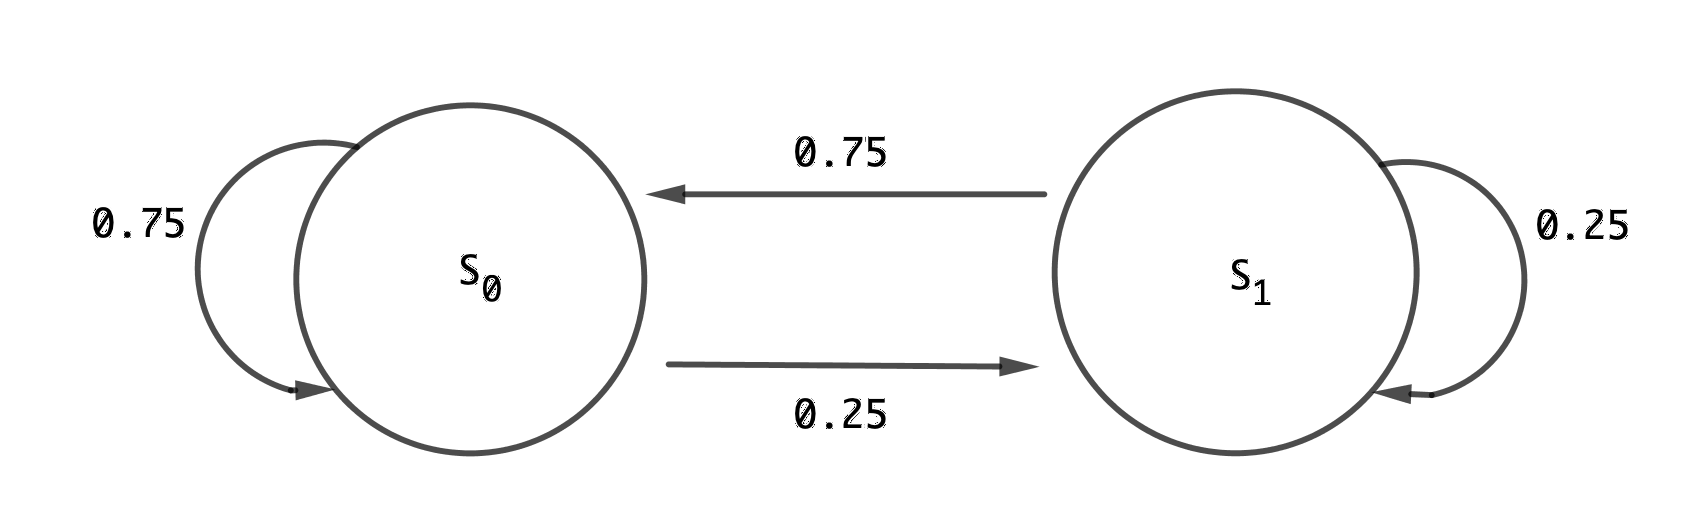
\includegraphics[width=\textwidth]{simple_markov_proc.png}
\caption{Simple Markov Process}
\label{fig:simplemarkov}
\end{figure}

When we repeatedly apply one-step transition probabilities this generalises to n-step transition probabilities [Bol06]. Let us denote $p_{ij}^{(n)}(k,l)$ as the probability that the Markov chain transitions from state $i$ at time $k$ to state $j$ at time $l$ in $n = k-l$ steps. Thus, we achieve the following equation that represents this: 

\begin{equation}
    p_{ij}^{(n)}(k,l)=P(X_l=j|X_k=i), 0 \leqslant k \leqslant l
\end{equation}

Using this equation, we can then compute the n-step transition probabilities recursively from the one-step transition probabilities [Bol06]. The transition of the process from state $i$ to state $j$ can be split into sub-transitions from state $i$ at time $k$ to an intermediary state $h$ at time $m$, and then from there we can say independently of the previous path that led to that state, from state $h$ to state $j$ at time $l$, where $k < m < l$ and $n = l-k$. This leads to the system of Chapman-Kolmogorov equations: 

\begin{equation}
    p_{ij}^{(n)}(k,l) = \sum_{h \in S} p_{ih}^{(m-k)}(k,m)p_{hj}^{(l-m)}(m,l), 0 \leq k < m < l
\end{equation}

The Chapman-Kolmogorov equations can then be simplified in the case of homogeneous discrete-time Markov Chains to the following equation: 

\begin{equation}
    p_{ij}^{(n)} = \sum_{h \in S} p_{ih}^{(m)}p_{hj}^{(n-m)}, 0 < m < n
\end{equation}

which can subsequently be simplified again when we consider the case where $m=1$:

\begin{equation}
    p_{ij}^{(n)} = \sum_{h \in S} p_{ih}^{(1)}p_{hj}^{(n-1)}
\end{equation}

We can then re-write these equations in terms of the matrices of the n-step transition probabilities. We can set $\mathbf{P}^{(n)} = \{p_{ij}^{(n)}\}$, and then for the case in which $m=1$ we get the equation: 

\begin{equation}
    \mathbf{P}^{(n)} = \mathbf{P}^{(1)}\mathbf{P}^{(n-1)}
    \label{eqn:nstepP}
\end{equation}

Therefore, the n-step transition probability matrix can be computed by using the $(n-1)$ fold multiplication of the one-step transition matrix by itself. [Bol06]. We can then consider the example from Figure \ref{fig:simplemarkov} and compute the 4-step transition proabilities from the one-step transition probability matrix. We have that: \[ \mathbf{P}^{(1)} = \left( \begin{array}{cc}
0.75 & 0.25 \\
0.75 & 0.25 \end{array} \right)\]

therefore we can say from Equation \ref{eqn:nstepP} that $\mathbf{P}^{(4)} = \mathbf{P}^{(1)} \mathbf{P}^{(3)} = \mathbf{P}^2 \mathbf{P}^{(2)} = $ \[\left( \begin{array}{cc}
0.75 & 0.25 \\
0.75 & 0.25 \end{array} \right)^2 \mathbf{P}^{(2)} = \left( \begin{array}{cc}
0.75 & 0.25 \\
0.75 & 0.25 \end{array} \right) \mathbf{P} \mathbf{P}^{(1)} = \left( \begin{array}{cc}
0.75 & 0.25 \\
0.75 & 0.25 \end{array} \right)\]

This example is off-putting because in our simple Markov Process example shown in Figure \ref{fig:simplemarkov} we have a transition matrix $\mathbf{P}$ which is idempotent, therefore we have $\mathbf{P}^n = \mathbf{P}$ no matter which value of $n$ that we choose with the condition that $n$ is a positive integer [Har97]. A different choice of Markov Process would yield more satisfying and visually significant results, however the theory is still correct. \\

Our current goal is to compute the pmf of the random variable $X_n$, which we evaluate from the probabilities $v_i(n)=P(X_n = i)$ that the discrete-time Markov Chain is in state $i$ at time step $n$. These probabilities are called transient state probabilities at time step $n$, and they allow us to derive desired performance measures of our Markov Process [Bol06]. If we know the $n$-step transition probability matrix $\mathbf{P}^{(n)}$, then the vector of state probabilities at time $n$ can be computed by un-conditioning $\mathbf{P}^{(n)}$ on the initial probability vector $\mathbf{v}(0) = (v_0(0), v_1(0),...,v_n(0))$ in the following fashion: 

\begin{equation}
    \mathbf{v}(n) = \mathbf{v}(0)\mathbf{P}^{(n)} = \mathbf{v}(n-1) \mathbf{P}
\end{equation}

An important aspect of homogeneous discrete-time Markov Chains are stationary probability vectors. State probabilities $\mathbf{v} = (v_0,v_1,...,v_n)$ are said to be stationary if any transitions of the underlying DTMC according to the one-step transition probabilities $\mathbf{P}=\{p_{ij}\}$ have no effect on these state probabilities. That is, $v_j = \sum_{i \in S} v_i p_{ij}$ holds for all states $j \in S$. Note that more than one stationary pmf can exist for a given, unrestricted DTMC. Stationary probability vectors can be represented in matrix form as follows:

\begin{equation}
    \mathbf{v} = \mathbf{v} \mathbf{P}, \: \sum_{i \in S} v_i = 1.
\end{equation}

We can take the analysis of Markov Processes much further by exploring them in significantly more detail. Much of the background reading for this project was focused on specific nuances of Markov Processes, how they work, how they can be applied to real-life situations and the mathematical analysis of specific examples. The work in this section just dabbles in an introduction to Markov Processes, and provides essential information that we will need later when we discuss queueing theory. Now that we have explored Markov Processes in sufficient, albeit very limited, detail, we can move onto single station queueing systems and Markov Arrival Processes; which are the next steps in understanding queueing networks. 

\section{Queueing Networks}

\subsection{Single Station Queueing Systems}

The information from this chapter has been summarised from [Bol06], [Kle76], [Coh82] and [Sho18]. Figure \ref{fig:simplequeue} shows a single station queueing system. This contains a queueing buffer of finite or infinite size and $m \geq 1$ servers, where  $m \in N^+$. We will use the terms single station queueing system, service station and node interchangeably.

\begin{figure}[h!]
\begin{center}
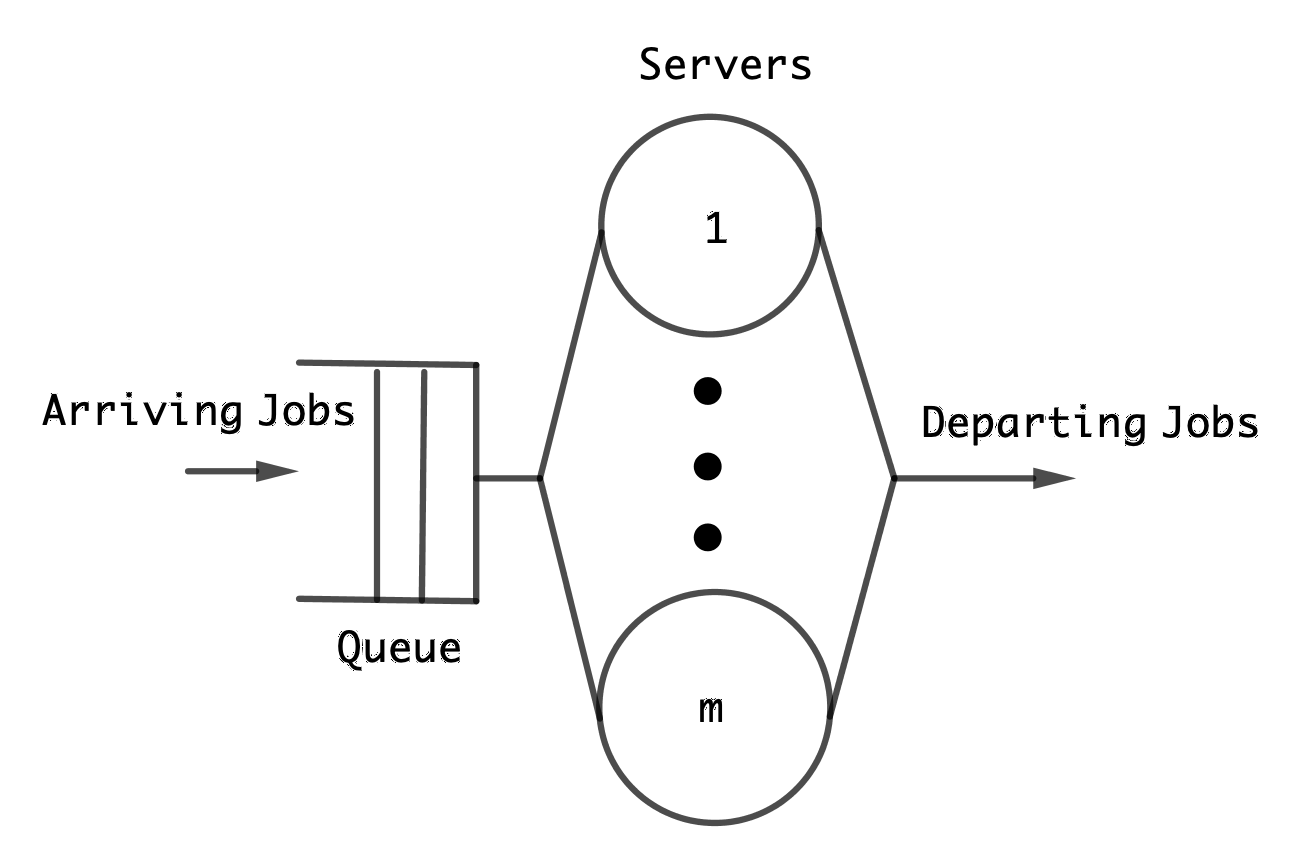
\includegraphics[width=90mm, scale=0.5]{Single_Queueing_System_Diagram.png}
\caption{Single Queueing System with m servers}
\label{fig:simplequeue}
\end{center}
\end{figure}

Each server can serve only one customer at a time [Bol06]. Therefore, we can say that each server is either in a `busy' or an `idle' state. [Bol06]. The buffer process is in place in case all of the servers are busy when a customer arrives in the queue. If this is the case, and there is buffer space available, the newly arriving customer is added to the buffer. When a different customer that is currently in service departs a server, one of the customers in the buffer is selected to proceed to be serviced by a queueing discipline. An additional description of an elementary queueing system is an arrival process, which can be categorized by its `sequence of inter-arrival time random variables $\mathbf{A} = \{A_1, A_2, ... , A_n \}$' [Bol06]. A common assumption on the sequence of inter-arrival times is that they are identically and independently distributed [Kle76]. The distribution of inter-arrival times can be continuous or discrete [Coh82]. The average inter-arrival time is denoted by an expectation: $E[\mathbf{A}] = T_A$, and the average arrival rate is denoted by its reciprocal: $\lambda = 1/T_A$ [Sho18]. The most widely used inter-arrival time distribution is the exponential distribution, which results in a Poisson arrival process [Bol06]. \\

Furthermore, the sequence of service times of successive jobs also needs to be specified, and is denoted by the sequence $\mathbf{B} = \{B_1, B_2, ... , B_3 \}$ [Bol06]. We follow a similar assumption in that this sequence is also a set of independent random variables with a common distribution function [Kle76]. The mean service time is denoted by $E[\mathbf{B}] = T_B$ and the service rate $\mu$ is the reciprocal: $\mu = 1/T_B$. 

\subsubsection{Notation for Elementary Queueing Systems}

The notation that we will use when discussing elementary queueing systems is the `Kendall Notation' [Bol06]. Kendall notation describes queueing systems in the following fashion: A/B/m - queueing discipline [Bol06], where A describes the distribution of the inter-arrival times, B denotes the distribution of the service times, and m denotes the amount of servers ($m \geq 1$). The following symbols are commonly used for A and B [Bol06]: 

\begin{itemize}
    \item $M$: Exponential distribution
    \item $E_k$: Erlang distribution with k phases
    \item $H_k$: Hyperexponential distribution with k phases
    \item $C_k$: Cox distribution with k phases 
    \item $D$: Deterministic distribution 
    \item $G$: General distribution 
    \item $GI$: General distribution with independent arrival times 
\end{itemize}

In many circumstances, we are interested in arrival processes where successive arrivals are correlated. Such non-GI arrival processes include the Markov Arrival Process, which we will go into further detail in the next chapter. \\

The selected queueing discipline for our system determines which jobs are selected from the queue to be processed by the servers. Commonly used queueing disciplines are shown below [Bol06]: 

\begin{itemize}
    \item FCFS (First Come First Served): this is the default queueing system if none is specified
    \item LCFS (Last Come First Served)
    \item SIRO (Service In Random Order)
    \item RR (Round Robin)
    \item PS (Processor Sharing)
    \item IS (Infinite Server)
    \item Static Priorities 
    \item Dynamic Prioirities 
    \item Preemption
\end{itemize}

\subsubsection{Performance Metrics for Queueing Systems}

We can analyse queueing systems mathematically to determine their performance metrics. Queueing models are dynamic, therefore their performance metrics vary over time. A system is in a steady state if all the transient behaviour of a system has ended or settled down, and the performance metrics are independent of time [Bol06]. When a system is in this state, it is said to be in statistical equilibrium, and is called a stable system [Bol06]. This situation occurs when the rate of jobs entering the system is equal to the rate of jobs leaving the system. To find solutions for general queueing systems we can use Markov Chain techniques. The generation and solution of large Markov chains are automated via stochastic reward nets [Bol06].

We will now discuss the most crucial performance metrics for queueing systems: 

\begin{itemize}
    \item The probability that there are a certain number of jobs currently in the system: $\pi_k = P$[there are $k$ jobs currently in the system].
    \item Utilization $\rho$: let $\lambda$ denote the arrival rate of the system, $m$ denote the amount of servers, and let $\mu$ denote the service rate of the system. Then, $\rho = \frac{\lambda}{m \mu}$. If $\rho < 1$ then the system is stable.
    \item Throughput $\lambda$: this metric is defined as the mean number of jobs that have completed being processed by the system in a single unit of time, which is known as the departure rate. The throughput is given by $\lambda = m.\mu.\rho$.
    \item Response time T: the total time a job spends in the system. 
    \item Waiting time W: the time a job spends in the buffer queue. We have that the response time is the sum of the waiting time and the service time. W and T are usually random numbers, so we can use their mean for analysis: $T = W + 1/\mu$
    \item Queue length Q: the number of jobs waiting in a buffer queue at a certain station.
    \item Average queue length $E[Q] = \lambda W$: the average number of jobs waiting in a queue for a certain station.
    \item Number of jobs in a system K: the population of jobs in the system.
    \item Mean number of jobs in a System $E[K] = \sum_{k=1} k.\pi_k = \lambda T$: the mean population of jobs in a system.
\end{itemize}

\subsection{Markovian Queues}

In this section we will explore 3 examples of queueing systems that follow a Markovian Process model. The information from this chapter has been summarised from [Bol06], [Cha01], [Bou11] and [Par08]. 

\subsubsection{M/M/1 Queue}

For the M/M/1 Queue the arrival process and the service times are exponentially distributed. Additionally, there is only one server. We use the notation $\lambda$ for the arrival rate, and $\mu$ for the service rate. As there is only a single server, we can treat the arrival rate as a `birth rate' and the service rate as the `death' rate [Bol06]. We can assume that $\lambda < \mu$ such that the underlying continuous Markov Process is ergodic and in a stable condition. Consequently, we can obtain the steady-state probability that the system is empty [Bol06]: 

\begin{equation}
    \pi_0 = \frac{1}{1 + \sum_{k = 1}^{\infty} \prod_{i = 0}^{k-1} \frac{\lambda}{\mu}} = \frac{1}{1 + \sum_{k = 1}^{\infty} (\lambda / \mu)^k}
\end{equation}

which subsequently can be simplified to the expression: 

\begin{equation}
    \pi_0 = \frac{1}{1 + \frac{\lambda / \mu}{1 - \lambda / \mu}} = 1 - \frac{\lambda}{\mu}
\end{equation}

The next step is to find the probability that there are $k$ jobs in the system. We have that: 

\begin{equation}
    \pi_k = \pi_0 (\lambda / \mu)^k = \left( 1 - \frac{\lambda}{\mu} \right).\left(\frac{\lambda}{\mu} \right)^k
\end{equation}

Subsequently, we can re-write this equation using the definition of the utilization as follows: 

\begin{equation}
    \pi_0 = 1 - \rho
\end{equation}

\begin{equation}
    \label{eqn:pmfutil}
     \pi_k = (1-\rho)(\rho)^k
\end{equation}

Equation \ref{eqn:pmfutil} shows the probability mass function of the geometric random variable. We can then plot this solution to show the pmf for each value of $k$ in the range $0-8$, which is shown in Figure \ref{fig:pmfgraph}. We have set the value of $\rho$ to be 0.5. 

\begin{figure}[h!]
\begin{center}
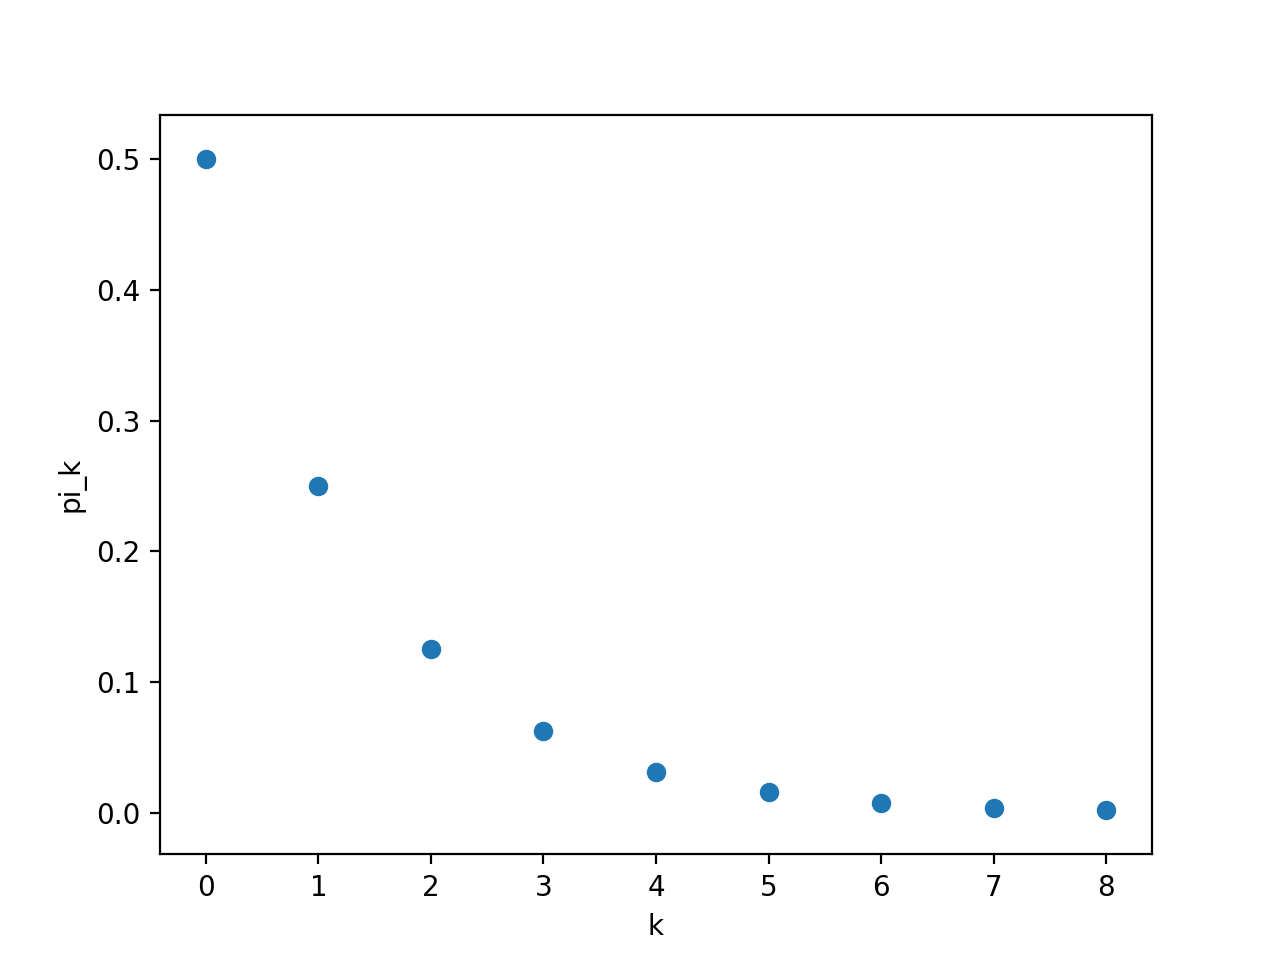
\includegraphics[width=100mm, scale=0.5]{Solution_for_pi_k.png}
\caption{Solution for $\pi_k$ for the M/M/1 Queue when $\rho = 0.5$}
\label{fig:pmfgraph}
\end{center}
\end{figure}

Additionally, and in a similar fashion, we can compute and graph the mean value of jobs in the system for different values of $\rho$ [Bol06]. We have that the average number of jobs is calculated using: 

\begin{equation}
    E[K] = \frac{\rho}{1-\rho}
\end{equation}

and Figure \ref{fig:mean_value_jobs_graph} shows the graph of the mean value of jobs for various values of $\rho$ where $0 \leq \rho < 1$. The behaviour shown in this graph is typical of of all queueing systems [Bol06]. 

\begin{figure}[h!]
\begin{center}
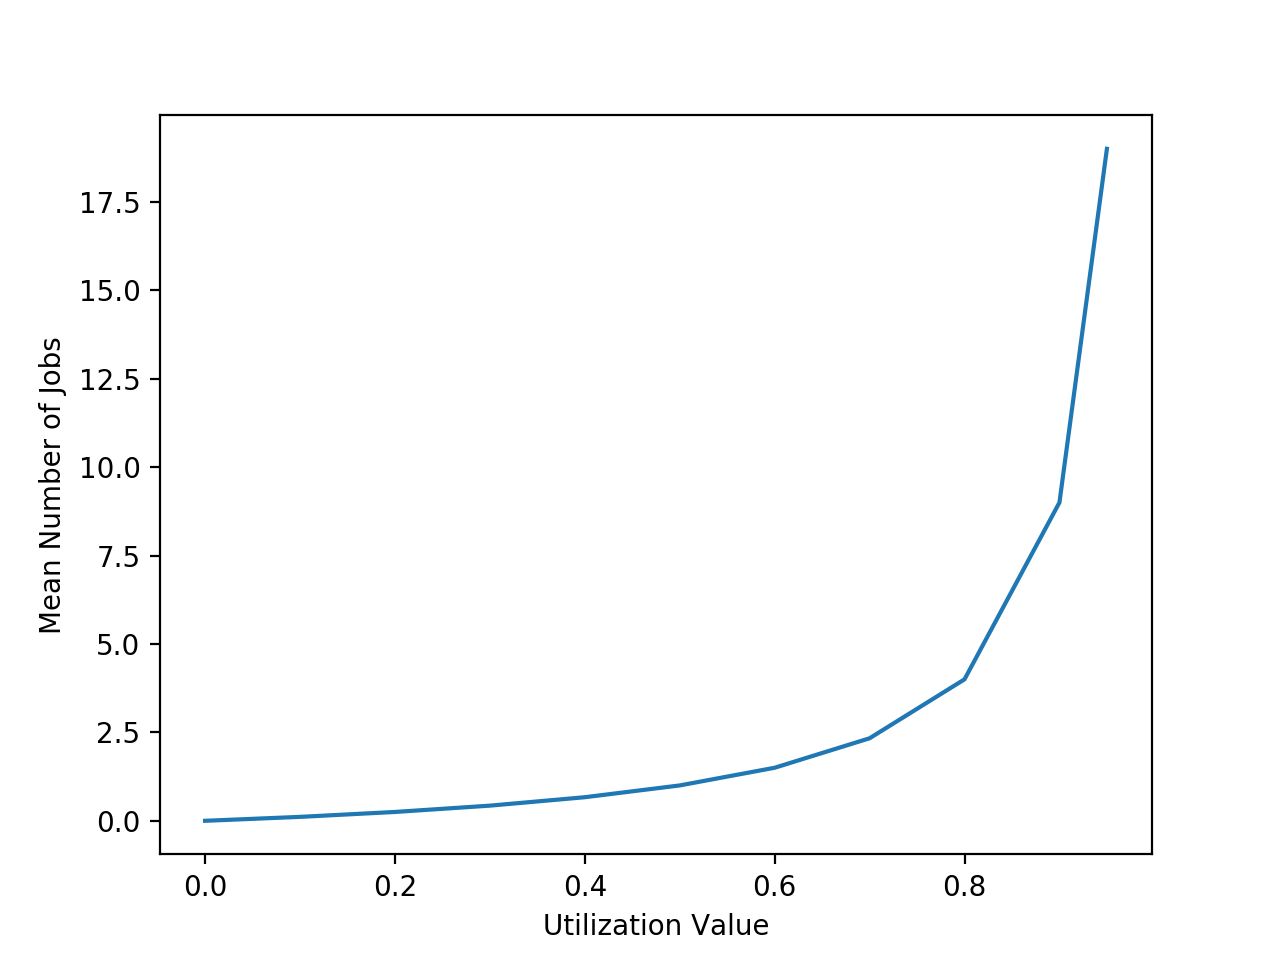
\includegraphics[width=100mm, scale=0.5]{Mean_value_jobs_util_real.png}
\caption{Mean number of Jobs in M/M/1 Queue}
\label{fig:mean_value_jobs_graph}
\end{center}
\end{figure}

The variance of the number of jobs in a system is denoted as $\sigma_K^2 = \rho/(1-\rho^2)$, with the coefficient of variation written as $c_K = \sigma_k / K = 1/\sqrt{\rho}$ [Bol06]. We can thus find equations for the mean response time $E[T]$, the mean waiting time $E[W]$ and the mean queue length $E[Q]$. We have that: 

\begin{equation}
    E[T] = \frac{1/\mu}{1-\rho}
\end{equation}

\begin{equation}
    E[W] = \frac{\rho/\mu}{1-\rho}
\end{equation}

\begin{equation}
    E[Q] = \frac{\rho^2}{1-\rho}
\end{equation}

Finally, we can find a relation for the response time distribution if we let the queueing discipline be First Come First Served. We consider the response time to be a sum of $k+1$ independent exponentially distributed random variables: $X_1 + X_2 + ... +X_k + X_{k+1}$, where $X$ is the service time and of the tagged job, $X_1$ is the remaining service time of the job in service, and $X_2, ..., X_k$ are the service times of the jobs in the queue [Bol06]. Each of these is exponentially distributed with parameter $\mu$. The Laplace-Stieljtes transform (LST) of the exponentially distributed service time is: 

\begin{equation}
    L_X(s) = \frac{\mu}{\mu + s}
\end{equation}

therefore we can express the conditional LST of the response time as: 

\begin{equation}
    L_{T|K}(s|k) = \left(\frac{\mu}{\mu + s} \right)^{(k+1)} .
\end{equation}

We can then use the steady state probabilities to do unconditioning, resulting in an LST of the response time as: 

\begin{equation}
    L_T(s) = \frac{\mu (1 - \rho)}{s + \mu (1 - \rho)}
\end{equation}

hence, the response time T is exponentially distributed with the parameter $\mu (1 - \rho)$:

\begin{equation}
    F_T(x) = 1 - e^{-\mu (1 - \rho) x}
\end{equation}

with a variance of:

\begin{equation}
    var(T) = \frac{1}{\mu^2 (1 - \rho)^2}
\end{equation}

and the distribution for the waiting time is shown below: 

\begin{equation}
F_W(x) = 
    \begin{cases}
    1-\rho & x = 0, \\
    1 - \rho e^{-\mu (1-\rho) x} & x > 0. \\
    \end{cases}
\end{equation}

We can then find the probability that an arriving job does not have to wait in the queue by computing:

\begin{equation}
    F_W(0) = P(W = 0) = 1 - \rho.
\end{equation}

\subsubsection{M/M/m Queue}

We will now look at the example of one more Markovian Queue, which is the M/M/m queue. This is similar to the M/M/1 queue, but instead of having only 1 server we now have $m \geq 1$ servers. The arrival rate $\lambda$ and service rate $\mu$ can be seen for each server in Equation \ref{eqn:arrival-service}: 

\begin{equation}
    \label{eqn:arrival-service}
    \lambda_k = \lambda
\end{equation}
$$ \mu_k = k . \mu $$ 

where $k \leq m$. The condition for a queueing system to be stable, where the underlying CTMC is ergodic, is $\lambda < \mu m$. The steady state probabilities are as follows for $0 \leq k \leq m$: 

\begin{equation}
    \pi_k = \pi_0 \prod_{i = 0}^{k-1} \frac{\lambda}{(i+1)\mu} = \pi_0 \left(\frac{\lambda}{\mu} \right) ^k . \frac{1}{k^2}
\end{equation}

The utilization for a single server is expressed as follows for $0 \leq k \leq m$: 

\begin{equation}
    \pi_k = \pi_0 \frac{(m \rho)^k}{k!}
\end{equation}

where:

\begin{equation}
    \pi_0 = \left[\sum_{k=0}^{m-1} \frac{(m \rho)^k}{k!} + \frac{(m \rho)^m}{m!} \frac{1}{1-\rho} \right ]^{-1}.
\end{equation}

The steady state probability that a customer has to wait in the queue is given by the expression: 

\begin{equation}
    P_m = P(K \geq m) = \sum_{k=m}^{\infty} \pi_k = \frac{(m \rho)^m}{m!(1-\rho)}.\pi_0
\end{equation}

where $K$ denotes the total number of jobs in the system. We can similarly find the mean number of jobs in the system using the formula: 

\begin{equation}
    E[K] = m \rho + \frac{\rho}{1-\rho} P_m.
\end{equation}

The mean queue length is given by:

\begin{equation}
    E[Q] = \frac{\rho}{1-\rho}  P_m
\end{equation}

and the formula for the distribution of the waiting time is given by: 

\begin{equation}
    F_W(x) =
    \begin{cases}
    1-P_m & x = 0, \\
    1 - P_m e^{-m \mu (1-\rho) x} & x > 0. \\
    \end{cases}
\end{equation}

The mean number of jobs and the mean queue lengths for various values of $m$ and for two values of $\rho$ are shown respectively in Figures \ref{fig:mean_number_jobs_M_M_m} and \ref{fig:mean_queue_length_M_M_m}. From observing Figures \ref{fig:mean_number_jobs_M_M_m} and \ref{fig:mean_queue_length_M_M_m}, we notice that as the number of servers increases the mean number of jobs increases and the mean queue length decreases, which is the expected result. 

\begin{figure}[h!]
\begin{center}
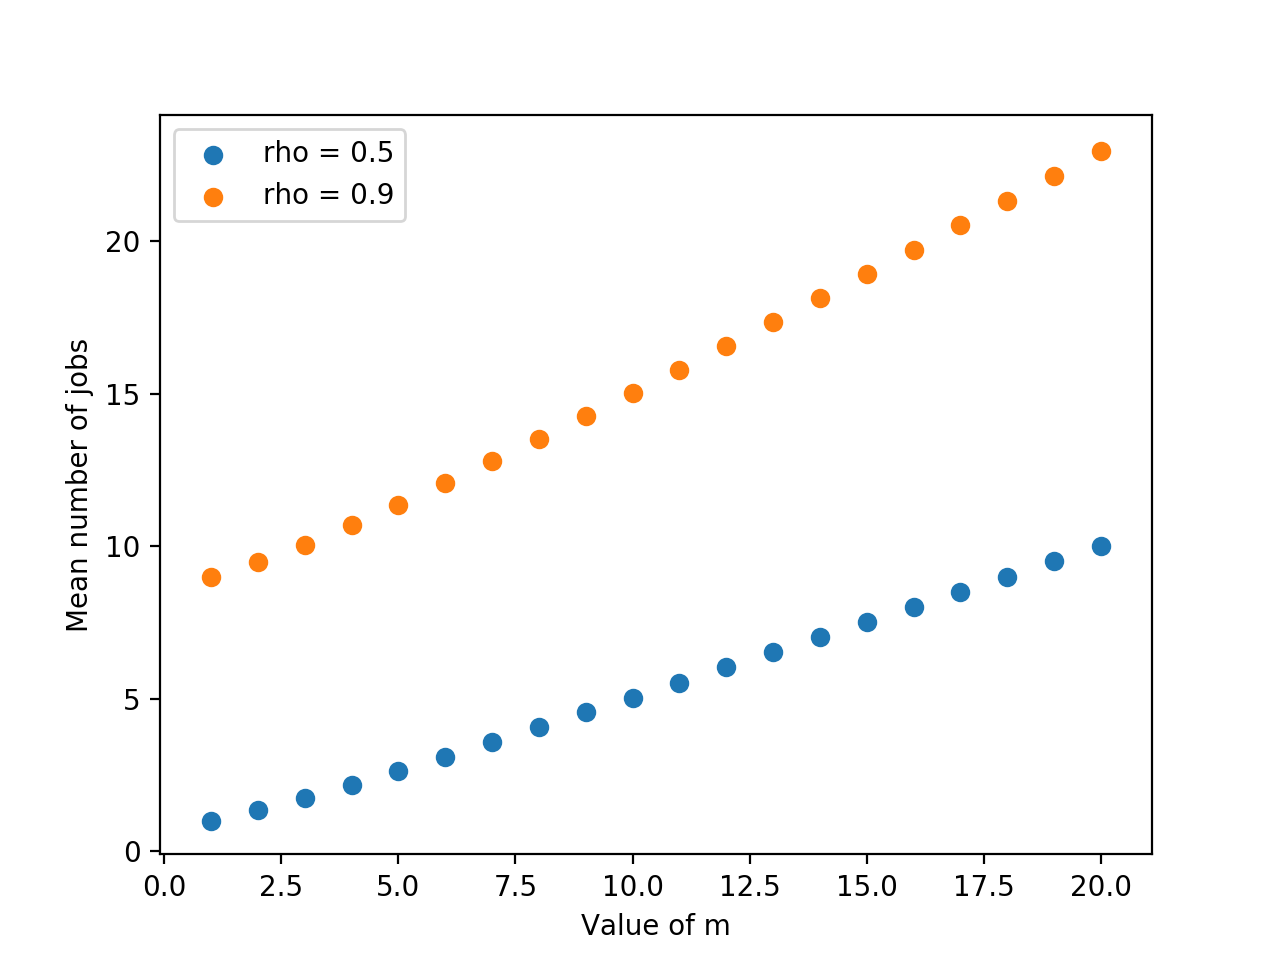
\includegraphics[width=100mm, scale=0.5]{mean_number_jobs_M_M_m.png}
\caption{Mean number of Jobs in M/M/m queue system as the number of servers vary}
\label{fig:mean_number_jobs_M_M_m}
\end{center}
\end{figure}

\begin{figure}[h!]
\begin{center}
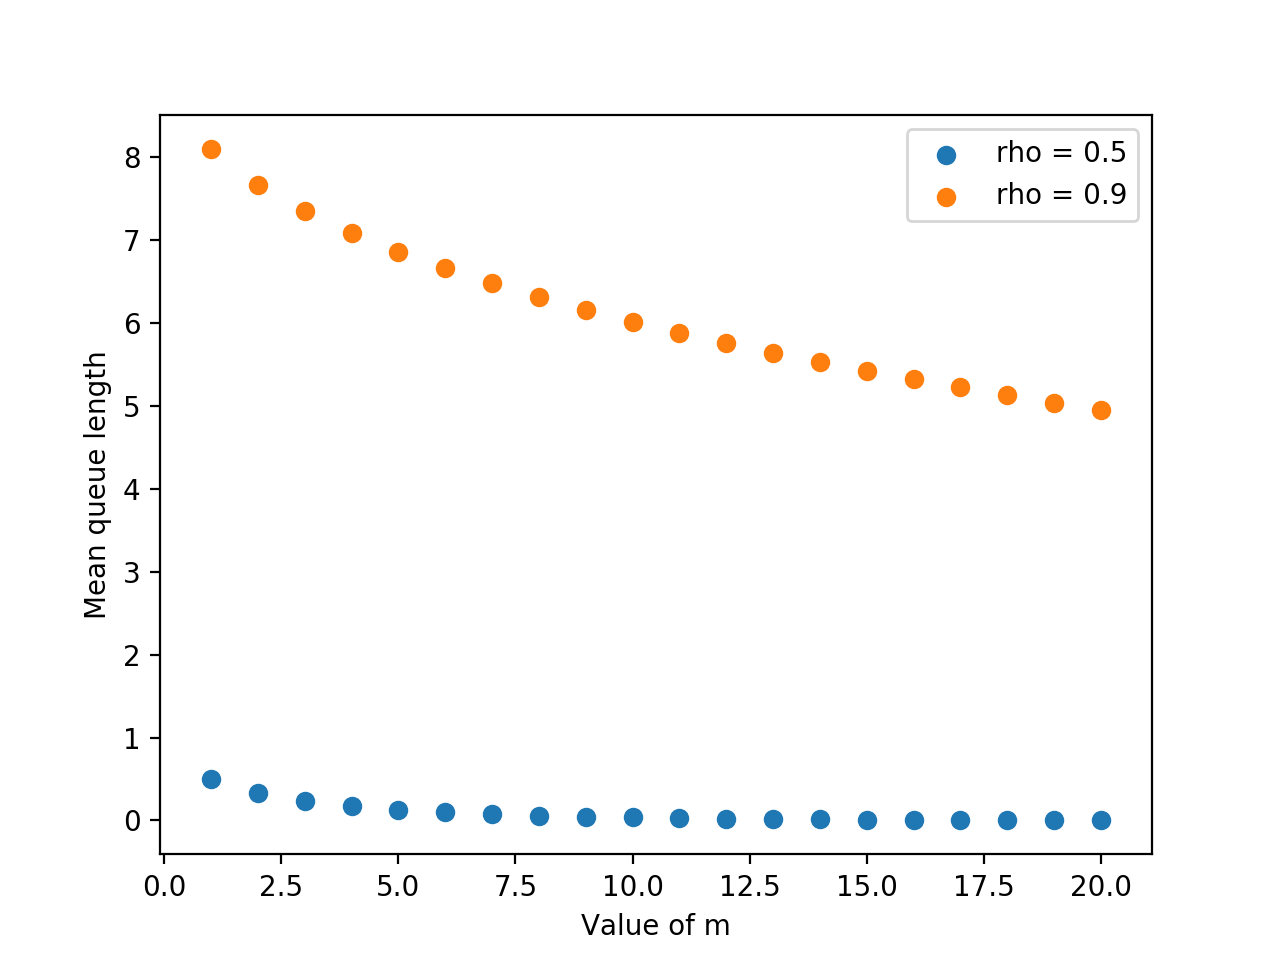
\includegraphics[width=100mm, scale=0.5]{mean_queue_length_M_M_m.png}
\caption{Mean queue length in M/M/m queue system as the number of servers vary}
\label{fig:mean_queue_length_M_M_m}
\end{center}
\end{figure}

\subsection{Queueing Networks}

We have covered elementary queueing systems, which will now let us understand the mechanics behind more complex queueing networks. The information from this chapter has been summarised from [Bol06], [Kle76], [Bou11], [Bal01] and [Sho18]. A queueing network consists of at least 2 service stations, and they are more suitable for representing the structure of real-life systems, which are usually more complicated than that of a system with only one service station [Bol06]. A station can also be called a node within the system, and represents a resource in the real system [Bol06]. Jobs within the system can be transferred from one node to any other node in the system, and also can be transferred back to the same node. A queueing network is either open or closed. An open network is when jobs can enter and leave the system from outside the network, and a closed network is when jobs are contained within the system, and can neither enter or leave the system [Bol06]. However, a network where a job enters the system as another job simultaneously leaves the system can be considered as a closed queueing network [Bol06].

\subsubsection{Examples of Queueing Networks}
Figure \ref{fig:openqueueingnetwork} shown an open queueing network that represents a simple computer system. Figure \ref{fig:centralservermodel} conveys a particular closed network that represents the behaviour of a multi-programming system. In this network, the node with service rate $\mu_1$ is the central server representing the CPU. The other nodes represent the other devices [Bol06]. 

\begin{figure}[h!]
\begin{center}
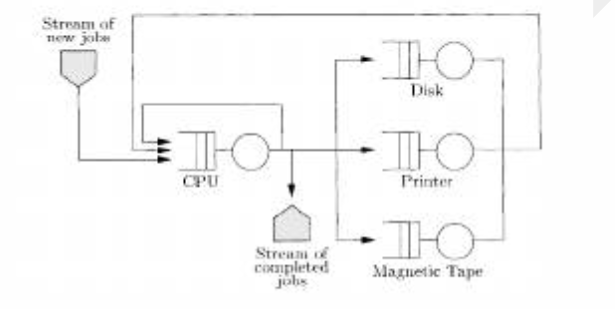
\includegraphics[width=100mm, scale=0.5]{open_computer_system.png}
\caption{Open queueing network conveying a computer system (taken from [Bol06])}
\label{fig:openqueueingnetwork}
\end{center}
\end{figure}

\begin{figure}[h!]
\begin{center}
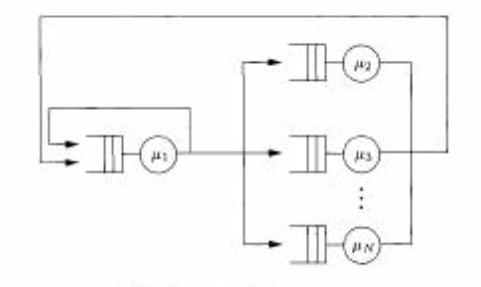
\includegraphics[width=100mm, scale=0.5]{closed_central_server_model.png}
\caption{Closed queueing network conveying a central server model (taken from [Bol06])}
\label{fig:centralservermodel}
\end{center}
\end{figure}

Figure \ref{fig:tandemmodel} shows a closed tandem model with 2 nodes. Figure \ref{fig:machinerepairmanmodel} represents a machine learning model, which can be used to convey the mechanics of several example systems. These include: a simple terminal system with M machines that represent the M terminals, and the repairman represents the computer; and a system in which M machines work independently and are repaired by a single repairmen if they fail [Bol06]. 

\begin{figure}[h!]
\begin{center}
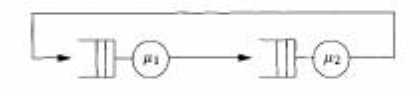
\includegraphics[width=100mm, scale=0.5]{closed_tandem_model.png}
\caption{Closed tandem model (taken from [Bol06])}
\label{fig:tandemmodel}
\end{center}
\end{figure}

\begin{figure}[h!]
\begin{center}
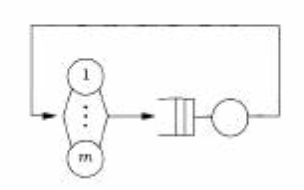
\includegraphics[width=100mm, scale=0.5]{machine_repairman_model.png}
\caption{Machine repairman model (taken from [Bol06])}
\label{fig:machinerepairmanmodel}
\end{center}
\end{figure}

\subsubsection{Definitions and Notation for Single-Class Queueing Networks}

In a very similar fashion to how we found definitions and defined notation for elementary queueing systems, we can do the same for more complex queueing networks. The information from this chapter has been summarised from [Bol06], [Kle76], [Bou11], [Bal01] and [Sho18]. We use the following symbols to describe single-class queueing networks [Bol06]:

\begin{itemize}
    \item N: the number of nodes.
    \item K: the constant number of jobs in the system.
    \item $(k_1,k_2,...,k_n)$: the state of the network.
    \item $k_i$: the number of jobs currently in the $ith$ node; for a closed network $\sum_{i=1}^{N} k_i = K$.
    \item $m_i$: the number of servers at the $i$th node.
    \item $\mu_i$: the service rate of the jobs at the $i$th node.
    \item $1/\mu_i$: the mean service time of the jobs at the $ith$ node.
    \item $p_{ij}$: the probability that a job processed by server $i$ is transferred to server $j$. This is referred to as the routing probability, where the node at server index $0$ in an open network represents the `external world' [Bol06].
    \item $p_{0j}$: the probability that a job entering from the external world is transferred to the $j$th node.
    \item $p_{i0}$: the probability that a job leaves the network straight after being processed by the $ith$ node.
    \item $\lambda_{0i}$: the arrival rate of jobs from the external world to the $i$th node.
    \item $\lambda$: the overall arrival rate from the external world to the open queueing network; $\lambda = \sum_{i=1}^{N} \lambda_{0i}$.
    \item $\lambda_i$: the overall arrival rate to the $i$th node.
    \item $e_i$: the mean number of visits of a job to the $i$th node; $e_i = \frac{\lambda_i}{\lambda}$ for $i = 1,2,...,N$.
\end{itemize}

\subsubsection{Performance Measures for Single-Class Queueing Networks}

The crucial problem that arises in queueing theory is calculating the steady state probabilities of all possible states in the system. This is because the mean values of all other performance measures can be calculated from the steady state probabilities of all possible states. The information from this chapter has been summarised from [Bol06], [Kle76], [Bou11], [Bal01] and [Sho18]. The most important performance measures of single-class queueing networks are as follows: \\

\textbf{Marginal Probabilities} $\pi_i(k)$: For closed queueing networks the marginal probabilities that the $ith$ node contains exactly $k$ jobs are calculated as in Equation \ref{eqn:marginalprobsincla}:

\begin{equation}
    \pi_i(k) = \sum_{\sum_{j=1}^{N}k_j = K \: \& \: k_i = k} \pi(k_1,k_1,...,k_N).
    \label{eqn:marginalprobsincla}
\end{equation}

Equation \ref{eqn:marginalprobsincla} is fairly complicated to understand, therefore it can be further explained in the following way: the $ith$ marginal probability denotes the sum of the probabilities of all possible states $(k_1,...,k_N)$, where $0 \leq k_i \leq K$, that satisfy the condition $\sum_{j=1}^{N} k_j = K$, where a fixed number, $k$, of jobs is given for the $ith$ node. Equation \ref{eqn:normalizationconstant} corresponds to the normalizing constant, which states that the sum of the probabilities of all possible states $(k_1,...,k_n)$ that satisfy the preceding condition that $\sum_{j=1}^{N} k_j = K$ must equal 1: 

\begin{equation}
    \sum_{\sum_{j=1}^{N} k_j = K} \pi(k_1, k_2,...,k_N) = 1
    \label{eqn:normalizationconstant}
\end{equation}

For open networks we have that:

\begin{equation}
    \pi_i(k) = \sum_{k_i = k} \pi(k_1,...,k_N)
\end{equation}

and a normalization condition of: 

\begin{equation}
    \sum \pi(k_1,...,k_N) = 1.
\end{equation}

\textbf{Utilization} $\rho_i$: The utilization of the $ith$ server node is given by Equation \ref{eqn:utilsingleserver}:

\begin{equation}
    \rho_i = \sum_{k=1}^{\infty} \pi_i k
    \label{eqn:utilsingleserver}
\end{equation}

which denotes the probability that the $ith$ node is busy. This can also be represented as: 

\begin{equation}
    \rho_i = 1 - \pi_i(0).
\end{equation}

Additionally, if the $ith$ node has multiple servers the utilization is defined as: 

\begin{equation}
    \rho_i = \frac{1}{m_i} \sum_{k = 0}^{\infty} min(m_i, k) \pi_i(k) = 1 - \sum_{k = 0}^{m_i - 1} \frac{m_i - 1}{m_i} \pi_i(k). 
\end{equation}

Furthermore, if the service rate is independent of the load we have that: 

\begin{equation}
    \rho_i = \frac{\lambda_i}{m_i \mu_i}
\end{equation}

\textbf{Throughput} $\lambda_i$: The throughput of a specific node indicates the rate at which jobs leave the node, and is specified by Equation \ref{eqn:throughputsingleclass}:

\begin{equation}
    \lambda_i = \sum_{k = 1}^{\infty} \pi_i(k) \mu_i(k)
    \label{eqn:throughputsingleclass}
\end{equation}

where we have that the service rate denoted by $\mu_i(k)$ is dependent on the number of jobs at the $ith$ node. For a node that is in equilibrium, we have that the arrival rate is equal to the throughput. \\

\textbf{Overall Throughput} $\lambda$: The overall throughput is the rate at which jobs leave the network, where this definition is only applicable to open networks. For an open network in equilibrium, we have that the overall throughput is: 

\begin{equation}
    \lambda = \sum_{i=1}^{N} \lambda_{0i}.
\end{equation}

For closed networks, the overall throughput is the throughput of a particular $ith$ node for which $e_i = 1$. Therefore, the overall throughput of a closed network is:

\begin{equation}
    \lambda = \frac{\lambda_i}{e_i}.
\end{equation} \\

\textbf{Mean Number of jobs} E[K]: The mean number of jobs at the $ith$ node is given by the equation: 

\begin{equation}
    E[K_i] = \sum_{k=1}^{\infty} k \pi_i(k).
\end{equation}

We can also write this equation in the following form, which we find by using Little's Theorem: 

\begin{equation}
    E[K_i] = \lambda_i E[T_i]
\end{equation}

where $E[T_i]$ is the mean response time of the $ith$ node. \\

\textbf{Average Queue Length} $E[Q_i]$: The mean queue length at the $ith$ node is given by:

\begin{equation}
    E[Q_i] = \sum_{k=m_i}^{\infty} (k-m_i)\pi_i(k)
\end{equation}

or using Little's Theorem this becomes: 

\begin{equation}
    E[Q_i] = \lambda_i E[W_i]
\end{equation}

\textbf{Mean Response Time} $E[T_i]$: The mean response time of jobs at the $ith$ node is given by the equation: 

\begin{equation}
    E[T_i] = \frac{E[K_i]}{\lambda_i}
\end{equation}

\textbf{Mean Waiting Time} $E[W_i]$: When the server rates are independent of the number of jobs at the $ith$ node, then the mean waiting time is given by:

\begin{equation}
    E[W_i] = E[T_i] - \frac{1}{\mu_i}
\end{equation}

This concludes all of the most important notations and performance measures for single-class networks. A similar analysis can be done for multi-class networks, which is a very important aspect of queueing theory. The notation is very similar for multi-class networks, but instead of just having one class of jobs we have $R$ job classes. For a detailed description of the notation and performance metrics of multi-class network, we ask the reader to examine the reference [Bol06]. We will discuss multi-class networks extensively in this paper, so it may be worthwhile to read up on this topic. 


\subsection{Product Form Queueing Networks}

Product form queueing networks are networks where the steady state solutions can be found without generating the underlying state space. The information from this chapter has been summarised from [Bol06], and [Bal01].

\subsubsection{Global Balance}

We can describe the behaviour of many queueing systems using continuous-time Markov chains. These are described by transition rates between the states of the corresponding model. If we have that the Markov chain is ergodic, then we have that a unique steady-state probability exists which is independent of the initial probability vector [Bol06]. We create a system of equations to determine the steady-state probability vector denoted by $\boldsymbol{\pi}$ is given by: $\boldsymbol{\pi Q} = \boldsymbol{0}$, where $\mathbf{Q}$ is the infinitesimal generator matrix of the CTMC [Bal01]. The conversation in steady state can be written as: 

\begin{equation}
    \sum_{j \in S} \pi_j q_{ij} = \pi_i \sum_{j \in s} q_{ij}, \: \forall i \in S
    \label{eqn:steadystateproduct}
\end{equation}

where $q_{ij}$ denotes the transition rate from state $i$ to state $j$. The global balance equation manipulates Equation \ref{eqn:steadystateproduct} to give [Bal01]: 

\begin{equation}
    \forall i \in S: \: \sum_{j != i} \pi_j \q_{ji} - \pi_i \sum_{j != i} q_{ij} = 0.
\end{equation}

The global balance equation is important because we can use them to realise important performance measures of the underlying queueing network [Bol06]. Additionally, global balance equations for large networks may be very expensive to use. In these situation, we use local balance instead. When all nodes of a system satisfy certain conditions, then local balance equations can be found to give important performance measures.

\subsubsection{Product Form}

The term product form was created to describe open and closed networks that have exponentially distributed inter-arrival and service times [Bol06]. Additionally, the queueing discipline at all service stations is assumed to be FCFS [Bal01]. Product form describes one of the most important results for queueing networks: the solution for the steady state probabilities can be expressed as a product of factors describing the state of each node [Bol06], [Bal01. We call this solution the product-form solution. There exist two characteristics that apply to queueing networks that have a product form solution other than the local balance characteristic [Bol06]:

\begin{itemize}
    \item M $\rightarrow$ M-Property (Markov implies Markov): A service station has this property if and only if the station transforms a Poisson arrival process into a Poisson departure process. If all nodes have this property, then the queueing network has a product form solution [Bol06]. 
    \item Station-Balance Property: A service discipline has this property if the service rates of a job that is served at a node are proportional to the probability that a job enters this position. If a network has this property it has a product form solution, but not the other way around [Bol06]. 
\end{itemize}

Notable queueing networks that have product form solutions are Jackson networks and Gordon-Newell networks [Bol06]. This concludes our description of the elementary background reading necessary for this project. In our main body of work, we include background research and theories that are very related to our technical implementations. We will now begin analysing machine learning methods applied to stochastic processes. Much more background reading could be detailed for this project, therefore if a reader is interested we would suggest reading through the following references: [Bol06], [Bal01], [Kle76], [Bou11], [Cas10] and [Sho18].

\section{EM Algorithms for Markov Arrival Processes}

In this chapter, we will discuss how how we can use EM algorithms to fit parameters of a Markov Arrival Process (MAP). An MAP defines a mathematical model for the time between job arrivals to a system [Cha01], [Hor05]. MAPs are a general class of Markov-modulated processes which are useful for fitting real workload traces which involve time varying characteristics [Cas10]. These type of traces are usually found in networks of computer systems, such as disk-drives [Cas10]. It is useful to use MAPs within our research for this project, as they are based on Markov chains. Therefore, it is simple to integrate them within queueing systems to describe metrics such as arrival or service processes [Cas10].\\

Within this chapter, we will build MAPs from queueing networks and then predict parameters of the resulting MAP using two EM algorithms that we will describe and implement. The first EM algorithm that we will discuss is detailed in the paper by Buccholz [Buc03]. We found that this implementation of the EM algorithm for MAP fitting did not give us very favourable results. Therefore, we also implemented an improved EM algorithm which is detailed in the papers by Hovarth et al. [Hor13], [Hor18] and Okamura [Oka08]. 

\subsection{Markov Arrival Processes}

Firstly, we will discuss some essential parameters associated with MAPs. We define $Z(t)$ to be an irreducible Markov chain with a generator matrix $\mathbf{Q}$ and state space $S = \{0,...,n-1\}$. To build the MAP from a queueing network is simple: simply set $\mathbf{Q}$ as the generator matrix of the queueing network that we want to build the MAP from. Additionally, we define two matrices $\mathbf{D_0}$ and $\mathbf{D_1}$ such that $\mathbf{D_1}$ is non-negative and $\mathbf{D_0} = \mathbf{Q} - \mathbf{D_1}$ [Tel07]. Two conditions that we impose on the matrix $\mathbf{D_1}$ are as follows: $\mathbf{Q}(x,y) - \mathbf{D_1}(x,y) \geq 0$ for $x \neq y$, and $\mathbf{D_1}(x,x) \geq 0$ [Buc03]. $\mathbf{D_0}$ describes the generator matrix of an absorbing state, whereas the matrix $\mathbf{D_1}$ contains transition rates that are accompanied by an arrival [Bol06]. We can consequently define the MAP as $M = \{\mathbf{D_0}, \mathbf{D_1}\}$ [Tel07], [Buc03], [Bol06]. The elements in $\mathbf{D}_0$ represent hidden transitions, and the elements in $\mathbf{D}_1$ represent observable transitions [Cha01]. \\

The solution of $\bm{\pi} \mathbf{Q} = 0$, where we have the condition $\bm{\pi}\mathbf{e}^T = 1$ when we solve for $\bm{\pi}$, is known as the steady state distribution [Tel07]. From this, we can compute the distribution straight after an arrival from the formula $\hat{\bm{\pi}} = \bm{\pi} \mathbf{ D}_{1}/(\bm{\pi} \mathbf{D}_1 \mathbf{e}{^T})$ [Buc03]. The $i$th conditional moments are given as the solutions to the set of equations $\mathbf{D_1m}^{(i)} = -i \mathbf{m}^{(i-1)}$ where $\mathbf{m}^{(0)} = \mathbf{e}^T$ and $\mathbf{m}$ denotes the conditional $ith$ moments [Tel07], [Hor05]. \\

The value of the distribution function at time $t$ is given by the function [Buc03]:

\begin{equation}
    FT(t) = \hat{\bm{\pi}} \mathbf{ D}_{0}[t] \mathbf{e^T} 
\end{equation}

where 

\begin{equation}
    \mathbf{D_0}[t] = e^{\mathbf{D_0}t} = \sum_{k=0}^{\infty}\beta(k, \alhpa t)(\mathbf{P_0})^k
\end{equation}

and $\mathbf{P_0} = \mathbf{D_0}/\alpha + \mathbf{I}$ and $\mathbf{P_1} = \mathbf{D_1}/\alpha$. Additionally, we have that $\beta(k, \alpha t) = exp(-\alpha t)(\alpha t)^k / k!$ and $\alpha \geq max_{x \in S}|\mathbf{D_0}(x,x)$ [Buc03].

\subsection{Computing the Likelihood of an Observed Sequence}

To apply expected-maximum algorithms to a MAP we first need a way to compute the transition likelihoods between states of the underlying Markov process. To do this we compute some form of joint densities or likelihoods rather than probabilities [Buc03].  We let $\mathbf{a}^{(i)}$ be a row vector that includes at position $x$ the likelihood of state $x$ immediately after observing the values $t_1,....,t_n$, where $i \leq m$ [Buc03]: 

\begin{equation}
    \mathbf{a}^{(i)} = \mathbf{a}^{(i-1)} \mathbf{D_0}[t_i]\mathbf{P_1} \: \text{with} \: \mathbf{a}^{0} = \hat{\bm{\pi}}
    \label{a_likelihood_eqn}
\end{equation}

In a similar fashion, we define the backward likelihood as [Buc03]:

\begin{equation}
    \mathbf{b}^{(i)} = \mathbf{D_0}[t_i]\mathbf{P_1}\mathbf{b}^{(i+1)}
    \label{b_likelihood_equation}
\end{equation}

with $\mathbf{b}^{(m)} = \mathbf{e}^T$. The normalized vector $\mathbf{b}^{(i)}$ is the probability of observing a sequence $t_i,...,t_m$ when we start in state $x$. We can thus find the quality of the approximation of an MAP to a trace denoted by $\bm{\tau}$ by measuring the value of the likelihood as follows: 

\begin{equation}
    d(\bm{\tau},M) = \alpha^m \mathbf{a}^{(m)} \mathbf{e}^T.
\end{equation}

where $\alpha$ is the rate used for randomization. Therefore the procedure for fitting to an MAP is to minimize the value of $d(\bm{\tau},M)$ which is a highly non-linear and complex optimization problem. We can thus try to solve this using machine learning methods, which is where the crux of this project lies. 

\subsection{Expected-Maximum Algorithm}

Within the EM algorithm we compute the transition likelihoods between states according to transitions with and without arrivals and use the normalized likelihoods to predict the transition probabilities in the matrices $\mathbf{P_0}$ and $\mathbf{P_1}$ [Buc03]. We define the forward likelihood as: $\mathbf{v}^{(i),k} = \mathbf{a}^{(i)} (\mathbf{P_0})^k$. We also define the backward likelihood as $\mathbf{w}^{(i),k} = (\mathbf{P_0})^k \mathbf{P_1} \mathbf{b}^{(i+1)}$. We can thus define two $n \times n$ matrices $\mathbf{X_0}$ and $\mathbf{X_1}$ which denote the transition likelihoods:

\begin{equation}
    \mathbf{X_0}^{(i)} (x,y) = \sum_{k=l_i}^{r_i - 1} \beta (k, \alpha t_i) \sum_{l=0}^{k-1} \mathbf{v}^{(i),l} (x) \mathbf{P_0} (x,y) \mathbf{w}^{(i),k-l-1}(y)
    \label{eqn:X_0}
\end{equation}

and 

\begin{equation} 
    \mathbf{X_1}^{(i)}(x,y) = \sum_{k=l_i}^{r_i} \beta (k, \alpha t_i) \mathbf{v}^{(i),k} (x) \mathbf{P_1}(x,y) \mathbf{b}^{(i+1)}(y)
    \label{eqn:X_1}
\end{equation}

where $r_i$ and $l_i$ denote the right and left truncation points respectively for the computation of the Poisson probabilities in the interval $[0,t_i)$ [Buc03]. The first matrix denotes the estimates for the likelihoods of the transitions without arrivals and the second the estimates for the likelihoods of transitions with arrivals. The likelihood values are collected in matrices as follows: 

\begin{equation}
    \mathbf{Y_0} = \sum_{i=1}^{m} \mathbf{X_0}^{(i)} 
\end{equation}

\begin{equation}
    \mathbf{Y_1} = \sum_{i=1}^{m} \mathbf{X_1}^{(i)} 
\end{equation}

where the normalized versions of these matrices denote the new estimates for $\mathbf{P_0}$ and $\mathbf{P_1}$. We therefore have found an iterative algorithm to fit the parameters of an MAP to a certain trace $\bm{\tau}$. 

\subsection{EM Algorithm Applied to Simple Markov Processes}

At this stage of our process, we explore an algorithm that attempts to fit the parameters of a Markov Arrival Process from a trace. To do this, we make use of MATLAB and the toolbox LINE [Lin20], as well as the description of the algorithm that is included in the research paper by Buccholz [Buc03]. This is the first machine learning algorithm that we will discuss with regards to stochastic processes. The aim of this algorithm is to take as an input a trace of inter-arrival times of jobs entering a network, and then fit parameters of an MAP to this trace. Therefore, the end result of this algorithm is to fit MAPs to real-world data, which could be collected from airport queuing times, traffic times, and many more. We will now describe the steps of the algorithm, as detailed in [Buc03].

\begin{enumerate}
    \item Take as the input of the algorithm a trace of inter-arrival times, denoted by: $\bm{\tau} = (t_1, t_2, ... , t_m)$. 
    \item Choose a value for the `basic rate', denoted by: $\alpha = min_{i=1,2,...,m} ((t_i)^{-1})$.
    \item Randomly choose values for the matrices $\mathbf{P_0} \geq 0$ and $\mathbf{P_1}\geq 0$, such that $\mathbf{P_0} + \mathbf{P_1}$ is stochastic.
    \item Repeat:
    \begin{enumerate}
    \item   compute $\hat{\bm{\pi}}$ and set $\mathbf{a^0} = \hat{\bm{\pi}}$;
    \item   for $i=1:m-1$ do:
    \begin{enumerate}
         \item       compute $\mathbf{a^{(i)}}$ via eqn (\ref{a_likelihood_eqn});
    \end{enumerate}
    \item   set $\mathbf{b}^m = \mathbf{e}^T$;
    \item for $i=m-1$ downto $1$ do:
    \begin{enumerate}
        \item compute $\mathbf{b}^{(i+1)}$ via eqn \ref{b_likelihood_equation};
        \item compute $\mathbf{X_0}$ and $\mathbf{X_1}$ via equations (\ref{eqn:X_0}) and (\ref{eqn:X_1}) respectively;
        \item set $\mathbf{Y_0} = \mathbf{Y_0}+\mathbf{X_0}^{(i)}$ and $\mathbf{Y_1} = \mathbf{Y_1} + \mathbf{X_1}^{(i)}$;
    \end{enumerate}
    \item set $\mathbf{P_0}^{old} = \mathbf{P_0}$ and $\mathbf{P_1}^{old} = \mathbf{P_1}$;
    \item normalize $\mathbf{Y_0}$ and $\mathbf{Y_1}$;
    \item set $\mathbf{P_0} = \mathbf{Y_0}$ and $\mathbf{P_1} = \mathbf{Y_1}$;
    \end{enumerate}
    \item Until max$\left(||\mathbf{P_0}-\mathbf{P_0}^{old}||, ||\mathbf{P_1}-\mathbf{P_1}^{old}||\right) \leq \epsilon$.
    \item Set $\mathbf{D_0} = \alpha \left(\mathbf{P_0} - \left(diag\left(\mathbf{P_0}\mathbf{e}^T + \mathbf{P_1} \mathbf{e}^T\right)\right)\right)$ and $\mathbf{D_1} = \alpha \mathbf{P_1}$.
    \item Output the MAP: $M = \{\mathbf{D_0}, \mathbf{D_1}\}.$
\end{enumerate}

\subsection{Discussion on the Improvements of the EM algorithm for MAP Fitting}

We find that the problem of parameter fitting for MAPs is complex as it is a highly nonlinear optimization problem. Therefore, there are many technical difficulties when implementing our EM algorithm. To assess the quality of our approximation, we choose any arbitrary MAP as input, create a trace from it to use in the algorithm, and then compute the value $d(\bm{\tau}, M) = \alpha^m \mathbf{a}^{(m)} \mathbf{e}^T$ [Buc03]. The procedure of MAP fitting maximizes this value [Tel07]. The higher this value, the better the approximation is. Therefore, in general it is a good approach to experiment with lots of different initial MAPs and perform the optimization for a whole trace and then observe the values of $d(\bm{\tau}, M)$ for the resulting MAPs [Buc03]. Additionally, we could also try to initially fit some characteristics of the trace within the algorithm to improve the MAP that results from this fitting [Buc03]. Furthermore, the complexity of the optimization depends upon the number of non-zero values in the matrices $\mathbf{P_0}$ and $\mathbf{P_1}$. If one of the values in these matrices is either set originally as 0 or becomes 0 during the iterative process, then that value will stay as 0 because the corresponding values for $\mathbf{X_0}(x,y)$ and $\mathbf{X_1}(x,y)$ as shown in equations \ref{eqn:X_0} and \ref{eqn:X_1} will remain 0. \\

Both the effort taken when using this algorithm and the quality of the fitting partially depends on the value that we choose for $\alpha$. In the algorithm proposed by Buccholz, we have that $\alpha$ is set to the inverse of the minimum value in the trace. Therefore, we generate an MAP that matches the first moment of the trace, however this may result in long execution times for the algorithm. If we choose a larger value for $\alpha$, then this would decrease the run time but may result in a worse approximation of the MAP [Buc03]. Let us assume that our algorithm has an output of an MAP that consists of the matrices $\mathbf{P_0}$ and $\mathbf{P_1}$. If we let $\bm{\pi}$ denote the stationary distribution of the MAP, then the first moment is given by: $E[T^{(1)}] = \bm{\pi} \mathbf{P_1} \mathbf{e}^T / \alpha$. We can then set $\mu_1$ as the first moment of the trace, and define a new value for $\alpha$ where $\alpha_{new} = \alpha E[T^{(1)}]/\mu_1$, such that we can yield a new MAP consisting of the matrices $\mathbf{P_0}$ and $\mathbf{P_1}$ where these are the same as the original MAP, but the matrices $\mathbf{D_0}$ and $\mathbf{D_1}$ are different [Buc03]. \\

A technical issue of the algorithm that we have proposed in Section 4.4 is that it can be very time consuming. One of the reasons for the taxing time constraints for this EM algorithm is that the $M = \{\mathbf{D}_0, \mathbf{D}_1\}$ matrix representation of an MAP is not unique [Hor18]. This has important practical consequences on our expectation-maximisation procedure. We may have that our algorithm flips back and forth between MAP representations that are close to identical with respect to the underlying MAP but have very different matrix representations [Hor18]. \\

We did in fact find that implementing the Buccholz algorithm gave us unfavourable results. Even though for some examples the predicted MAPs were of good quality, most of the time the algorithm would fall into a local optima. This is due to the following issues: this EM algorithm is too reliant on the initial conditions that we impose on $\mathbf{P}_0$ and $\mathbf{P}_1$, therefore we only got favourable results if we were lucky and our initial guesses of these matrices were good; the algorithm is a very complex non-linear optimization problem, therefore occasionally we would not get good results at all and find ourselves in a situation where the matrix values would all converge to 0; and the time taken for the algorithm to optimize was far too long. As a result of these issues, we abandoned our implementation of this algorithm in favour of an improved algorithm. Our findings of the results of this algorithm is backed by the research present in [Hor13], [Hor16] and [Oka08].  We have kept the theory behind this algorithm in this paper because it was a very important stepping stone to the improved algorithm, which gave us very favourable results. Also, the Buccholz algorithm implementation will be in the software folder so the reader can try it out for themselves. \\

To bypass the issues detailed above and to reduce the complexity of our computations we can use structurally restricted subclasses of MAPs [Hor13], which we will now discuss in more detail.

\subsubsection{ER-CHMM Structure of MAPs}

We will now discuss how we can use a specific structural subclass of an MAP to improve our EM algorithm. Using this restriction, we have that in the arrival process the inter-arrival times are Erlang distributed. Additionally, the inter-arrival times are modulated by a discrete-time hidden Markov chain [Hor13]. In this restriction, we have that the next state and inter-arrival time of the Markov chain are independent random variables, which is not necessarily the case with general MAPs. Interestingly, we still have that in general the inter-arrival times generated by an ER-CHMM Markov chain are still correlated [Hor16]. \\

We will now discuss the parameters involved in the ER-CHMM structure [Hor18], [Bra19]. We have the parameters: $\mathbf{r} = (r_1,...,r_N)$, $\bm{\lambda} = (\lambda_1,...,\lambda_N)$, and $\mathbf{T}= \{p_{ij}\}$, where $r_i$ denotes the $i$th order of the Erlang distribution branch, $\lambda_i$ denotes the rate of the $i$th Erlang distribution branch and, $\mathbf{T}$ denotes the $R \times R$ probability transition matrix of the discrete-time Markov chain that determines the branch providing the consecutive inter-arrival times. From the parameters of the branch, we have that the densities of the inter-arrival times generated by branch $i$ are shown in Equation \ref{eqn:branch_density} [Hor18], [Bra19]. 

\begin{equation}
f_i(x) = \frac{(\lambda_i x)^{r_{i}-1}}{(r_i-1)!} \lambda_i e^{-\lambda_i x}
\label{eqn:branch_density}
\end{equation}

We can consequently find the $\{\mathbf{D}_0, \mathbf{D}_1\}$ MAP representation from the parameters $\mathbf{r}$, $\bm{\lambda}$ and $\mathbf{T}$ [Oka08]. Let us define the $1 \times r$ initial vector and $r \times r$ transient generator of the order $r$ Erlang distribution with parameter $\lambda$ by Equations \ref{eqn:init_erlang} and \ref{eqn:trans_erlang} respectively [Oka08], [Hor18], [Bra19]: 

\begin{equation}
    \bm{\beta}(r) = [1,0,...,0]
    \label{eqn:init_erlang}
\end{equation}

\begin{equation}
    \mathbf{B}(r,\lambda) = \begin{bmatrix}
     -\lambda & \lambda & 0 & ... \\
     0 & -\lambda & \lambda & ... \\
     0 & 0 & ... & ... \\
     0 & 0 & 0 & -\lambda
    \end{bmatrix}
    \label{eqn:trans_erlang}
\end{equation}

then we have that the representation of the $\mathbf{D}_0$ and $\mathbf{D}_1$ matrices are shown in Equations \ref{eqn:D0_erlang} and \ref{eqn:D1_erlang} [Hor18], [Bra19]: 

\begin{equation}
    \mathbf{D}_0 = \begin{bmatrix}
     \mathbf{B}(r_1,\lambda_1) & ... & \mathbf{B}(r_1,\lambda_R)  \\
     \mathbf{B}(r_2,\lambda_1) & .. & \mathbf{B}(r_2,\lambda_R) \\
     ... & ... & ... \\
     \mathbf{B}(r_R,\lambda_1) & ... & \mathbf{B}(r_R,\lambda_R)
    \end{bmatrix}
    \label{eqn:D0_erlang}
\end{equation}

\begin{equation}
    \mathbf{D}_1 = \begin{bmatrix}
     -\mathbf{B}(r_1,\lambda_1) \mathbbm{1} .p_{1,1}.\bm{\beta}(r_1) & ... & -\mathbf{B}(r_1,\lambda_1) \mathbbm{1} .p_{1,R}.\bm{\beta}(r_R)   \\
     ... & ... & ... \\
     ... & ... & ... \\
     -\mathbf{B}(r_R,\lambda_R) \mathbbm{1} .p_{R,1}.\bm{\beta}(r_1)  & ... & -\mathbf{B}(r_R,\lambda_R) \mathbbm{1} .p_{R,R}.\bm{\beta}(r_R)
    \end{bmatrix}.
    \label{eqn:D1_erlang}
\end{equation}

From this representation of the matrices we can see one of the main reasons why the time complexity is reduced in this EM algorithm. For a normal representation of an MAP, the density function of the stationary inter-arrival time $f(x)$ and its $n$th moment $E(X^n)$ are described in Equations \ref{eqn:dens_norm_map} and \ref{eqn:nth_moment_map} [Oka08]:

\begin{equation}
    f(x) = \bm{\pi} e^{\mathbf{D}_0 x} \mathbf{D}_1 \mathbbm{1}
    \label{eqn:dens_norm_map}
\end{equation}

\begin{equation}
    E[X^n] = n! \bm{\pi}(-\mathbf{D}_0)^{-n} \mathbbm{1}
    \label{eqn:nth_moment_map}
\end{equation} 

where $\bm{\pi}$ denotes the stationary state distribution vector at arrival instants. Additionally, the joint densities are represented as follows [Bra19], [Hor13]:

\begin{equation}
    f(x_1,x_2,...,x_T) = \bm{\pi} e^{\mathbf{D_0}x_1}\mathbf{D}_1 \: ... \: e^{\mathbf{D}_0 x_T}\mathbf{D}_1 \mathbbm{1} = \bm{\pi} \prod_{k=1}^{T} \mathbf{A}[k] \mathbbm{1}
\end{equation}

where the matrix $\mathbf{A}$ is the crucial component of the joint density function. This matrix is computationally far less expensive in the ER-CHMM structure of an MAP because it does not rely on computationally heavy matrix exponential functions, and instead simplifies to scalar products of $p_{ij}$ and $f_i(x)$. We will briefly demonstrate this using a simple example. Let us take $\mathbf{r} = [3,1]$, and consequently find the $\mathbf{D}_0$, $\mathbf{D}_1$ and $\mathbf{A}$ matrices [Hor18]:

\begin{equation}
    \mathbf{D}_0 = \begin{bmatrix}
     -\lambda_1 & \lambda_1 & 0 & 0 \\
     0 & -\lambda_1 & \lambda_1 & 0 \\
     0 & 0 & -\lambda_1 & 0 \\
     0 & 0 & 0 & \lambda_2
    \end{bmatrix}
    \label{D0_comp_cheap}
\end{equation}

\begin{equation}
    \mathbf{D}_1 = \begin{bmatrix}
     0 & 0 & 0 & 0 \\
     0 & 0 & 0 & 0 \\
     p_{1,1} \lambda_1 & 0 & 0 & p_{1,2} \lambda_1 \\
     p_{2,1} \lambda_2 & 0 & 0 & p_{2,2} \lambda_2
    \end{bmatrix}
    \label{D0_comp_cheap}
\end{equation}

\begin{equation}
    \mathbf{A}(k) = e^{\mathbf{D}_0 x_k} \mathbf{D}_1 = \begin{bmatrix}
     p_{1,1} f_1(x_k) & 0 & 0 & p_{1,2} f_1(x_k) \\
     * & 0 & 0 & * \\
    * & 0 & 0 & * \\
     p_{2,1} f_2(x_k) & 0 & 0 & p_{2,2} f_2(x_k)
    \end{bmatrix}
    \label{D0_comp_cheap}
\end{equation}

where we we have irrelevant matrix values represented by $*$ because the phase is constrained to either 1 or 4 by the zero columns [Hor18]. As a result of this, we can use dimensionality reduction on the matrix $\mathbf{A}(k)$ by removing the zero values and the irrelevant matrix indices to give a size R matrix [Hor18]: 

\begin{equation}
    \mathbf{P}(k) = \begin{bmatrix}
     p_{1,1} f_1(x_k) & ... & ... & p_{1,R} f_1(x_k) \\
     ... & ... & ... & ... \\
     p_{R,1} f_R(x_k) & ... & ... & p_{R,R} f_R(x_k)
    \end{bmatrix}
\end{equation}

which we can consequently use to find the joint density function by Equation \ref{p-matrix_dens}:

\begin{equation}
    f(x_1,x_2,...,x_T) = \bm{\pi} \prod_{k=1}^{T} \mathbf{P}[k] \mathbbm{1}
    \label{p-matrix_dens}
\end{equation}

where $\bm{\pi}$ is the stationary distribution of the matrix $\mathbf{T}$. Hence, $\bm{\pi} \mathbf{T} = \bm{\pi}$ and $\bm{\pi} \mathbbm{1} = 1$. In this representation we have dimensional reduction where $R \leq N$, and we avoid expensive matrix exponential equations, therefore we can make our calculations less computationally expensive. 

\subsection{EM Algorithm for MAP Fitting Using ER-CHMM Structure of MAPs}

The fundamental aspect of this EM algorithm has not changed from the algorithm that we discussed before: we are trying to maximise the likelihood of the trace data, shown in Equation \ref{eqn:likelihood_erlang} [Oka08], [Hor18]:

\begin{equation}
    L(\bm{\tau},\mathbf{D}_0, \mathbf{D}_1) = \bm{\alpha} e^{\mathbf{D}_0 \tau_1} \mathbf{D}_1 e^{\mathbf{D}_0 \tau_2} \mathbf{D}_1 ... e^{\mathbf{D}_0 \tau_T} \mathbf{D}_1 \mathbbm{1} = \bm{\alpha} \prod_{k=1}^T \mathbf{A}(k) \mathbbm{1}
    \label{eqn:likelihood_erlang}
\end{equation}

where $\bm{\tau} = (\tau_1,...,\tau_T)$ denotes the trace. From this expression, the aim of the algorithm is to find the predicted matrices $\mathbf{D}_0$ and $\mathbf{D}_1$ that maximizes the likelihood $L$, such that:

\begin{equation}
    \mathbf{D}_0, \: \mathbf{D}_1 = argmax(L(\bm{\tau}, \mathbf{D}_0, \mathbf{D}_1)).
\end{equation}

When we use the ER-CHMM structure with orders $\mathbf{r}$ for our MAPs, our formulation changes slightly. We are now optimizing the likelihood as follows: 

\begin{equation}
    \bm{\lambda}, \mathbf{T} = argmax (L(\bm{\tau}, \bm{\lambda}, \mathbf{T}))
\end{equation}

where $L(\bm{\tau}, \bm{\lambda}, \mathbf{T}) = \bm{\pi} \prod_{k=1}^T \mathbf{P}(k) \mathbbm{1}$. It is important to note that from this representation, we can easily switch back to the $\mathbf{D}_0$ and $\mathbf{D}_1$ notation of the MAP using Equations \ref{eqn:D0_erlang} and \ref{eqn:D1_erlang}. Furthermore, the concepts introduced in this section are broad enough such that we can generalise to any MAP structure, regardless of restrictions. This is a crucial aspect as to why this EM algorithm implementation is such an improvement on the previous algorithm: it can generalise to all MAPs; it is faster and less computationally expensive; is less likely to fall into local optima; and in general it achieves higher likelihood values, which is verified by the references [Hor18], [Hor13] and [Oka08]. Before we delve into the depths of the algorithmic procedure, we will first define some important parameters that we need for the algorithm. This is similar to our previous EM algorithm, where we need to define backward and forward likelihood vector equations. We will then explore the E-step and M-step for our algorithm. \\

In this algorithm, we will use a structure of MAPs that is very similar to the ER-CHMM structure. We will use $M$ branches where branch $i$ consists of $r_i$ states connected in a row with the same transition rates $\lambda_i$. The branches will not quite represent Erlang distributuions, as we will not traverse all states of the branch before generating an arrival [Hor18]. When we have that a branch is selected to generate the next inter-arrival time, the initial state of the branch is determined by a probability vector [Hor18]. We will now define the forward and backward likelihood vectors that we will use in our procedure. We have the forward likelihood vector, denoted by $\mathbf{a}[k] = \{a_i[k], i=1,...,R\}$, $k=1,...,T$ and the backward likelihood vector $\mathbf{b}[k] = \{b_i[k], i=1,...,R\}$, $k = 1,...,T+1$. We can also note that the row vectors $\mathbf{a}[k]$ and column vectors $\mathbf{b}[k]$ have probabilistic interpretations, where $a_i[k]$ represents the density that $i$ is the state of the background discrete-time Markov Chain and the inter-arrival times $\tau_1,...,\tau_k$ are observed, and $b_j[k]$ is the density of observing inter-arrival times $\tau_k,...,\tau_T$ if the state of the background DTMC is $j$ initially. We can then define the equations that we use to update the forward and backward likelihoods recursively in our algorithm [Hor13], [Hor18]:

\begin{equation}
    a_i[k] = \begin{cases}
    \pi_i, & \text{for } k = 0 \\
    \sum_{j=1}^R a_j[k-1]f_j(\tau_k)p_{j,i}, & \text{for } 1 \leq k \leq T.
  \end{cases}
\end{equation}

\begin{equation}
b_i[k] = \begin{cases}
    \sum_{i=1}^R f_j(\tau_k)p_{j,i} b_i[k+1], & \text{for } 1 \leq k \leq T \\
    1, & \text{for } k = T+1.
  \end{cases}
\end{equation}

The likelihood can therefore be expressed as follows: 
\begin{equation}
    L(\bm{\tau}, \bm{\lambda}, \mathbf{T}) = \mathbf{a}[T] \mathbbm{1} = \bm{\pi} \mathbf{b}[1].
\end{equation}

Subsequently, we can define the estimates for the parameters $\bm{\lambda}$ and $\mathbf{T}$:

\begin{equation}
    \lambda_i^{,} = \frac{\sum_{k=1}^T r_i a_i[k-1]b_i[k]}{\sum_{k=1}^T \tau_k a_i[k-1]b_i[k]},
\end{equation}

\begin{equation}
    p_{i,j}^{,} = \frac{\sum_{k=1}^{T-1} a_i[k-1] f_i(x_k) p_{i,j} b_j[k+1]}{\sum_{k=1}^{T-1} a_i[k-1] b_i[k]}
\end{equation}

We also have that the estimates of the initial branch probabilities denoted by $\pi_i^{,}$ can be evaluated as: 
\begin{equation}
    \pi_i^{,} = \frac{\sum_{k=1}^T a_i[k-1]b_i[k]}{T.\mathbf{a}[T] \mathbbm{1}}.
\end{equation}

From the above equations we can interpret the process of the E-step and the M-step of our algorithm. The E-step consists of alternating the computation of the $\mathbf{a}[k]$ and $\mathbf{b}[k]$ vectors, while the M-step consists of computing the new estimates for $\bm{\lambda}'$, $\mathbf{T}'$ and $\bm{\pi}'$. Additionally, we can match the initial moments as discussed in previous sections, to give better predictions. We can now define the steps for our new and improved EM algorithm, as detailed in [Hor18], [Hor13], [Oka08], [Bra19]. \\

\textbf{Procedure: EM algorithm using ER-CHMM structure}

\begin{enumerate}
    \item Take as input to the algorithm the trace $\bm{\tau}$ and a value $r$ which determines the size of the orders of the Erlang distribution that we will use.
    \item Set $LogLi=-\infty$.
    \item Initialize $\mathbf{T} = \{p_{i,j}\}$ and $\lambda_i$.
    \item While $(LogLi-OLogLi)/LogLi > \epsilon$ do:
    \begin{itemize}
        \item Obtain vector $\bm{\pi}$.
        \item For $k = 1:K$ do:
        \begin{itemize}
            \item Compute and store conditional densities $f_i(\tau_k)$.
        \end{itemize}
        \item for $k=0:K$ do:
        \begin{itemize}
            \item Compute and store forward likelihoods $\mathbf{a}[k]$.
        \end{itemize}
        \item For $k=K:1$ do:
        \begin{itemize}
            \item Compute and store backward likelihoods $\mathbf{b}[k]$.
        \end{itemize}
        \item For $i=1:M$ do:
        \begin{itemize}
            \item Compute new estimate for $\lambda_i$.
        \end{itemize}
        \item For $i=1:M$ and $j=1:M$ do:
        \begin{itemize}
            \item Compute new estimate for $p_{i,j}$.
        \end{itemize}
        \item $OLogLi = LogLi$.
        \item $LogLi = \bm{\pi}.\mathbf{b}[0]$.
    \end{itemize}
    \item Calculate $\mathbf{D}_0$ and $\mathbf{D}_1$ from $\bm{\lambda}$, $\mathbf{r}$ and $\mathbf{T} =\{p_{ij}\}$.
    \item Return $MAP = \{\mathbf{D}_0,\mathbf{D}_1\}$.
\end{enumerate}

In our algorithm from the value of $r$ we take different combinations of the orders that sum to $r$ and repeat the algorithm for all possible combinations from the value. We then take the returned MAP from the order combination that gives the highest log-likelihood computation. 

\section{Experimental Validation of the EM Algorithm for MAP Fitting}

We can now explore the results and conclusions that can be drawn from our EM algorithm for MAP fitting. We will briefly discuss how the EM algorithm was implemented. Initially, we create a predetermined queueing network from which we can build an MAP. Subsequently, we generate a trace from the corresponding MAP. The consequent aim from the EM algorithm is to then try to fit a different MAP by using the generated trace, which we can subsequently compare to the actual MAP that generated it to see how accurate the algorithm is at fitting the parameters of the MAP. This is a very complex algorithm, as the optimization of the parameters of the MAP is a highly non-linear and non-convex problem. In our experimental validation we will consider many examples of MAPs built from different kinds of queueing networks, and analyse how well our algorithm can fit the parameters of the MAP from the generated traces in each example. \\

We will use certain metrics to evaluate the accuracy of our predicted MAP from the MAP that generated the trace. We will compare the mean and variance of each MAP and see how well they match, as well as comparing the auto-correlation of lag $k$ ($k \geq 1$) for each MAP. The auto-correlation of lag  $k$ is defined in Equation \ref{eqn:aclag}, and measures the correlation of values that are $k$ time periods apart [Buc03], [Hor05], [Cas10]. We have that $E[T^{(k)}] = \bm{\pi'} \mathbf{m}^{(i)}$ denotes the $k$th absolute moment [Tel07], [Cas10]. 

\begin{equation}
    E[\rho_k] = \frac{E[T^{(1)}] \bm{\pi} \left( (-\mathbf{D}_0^{-1} \mathbf{D}_1)^k \mathbf{m}^{(1)} - \mathbf{e}^T E[T^{(1)}] \right)}{E[T^{(2)}] - \left(E[T^{(1)}]\right)^2}
    \label{eqn:aclag}
\end{equation}

Additionally, we will compare the matrices $\mathbf{D}_0$ and $\mathbf{D}_1$ from both the real and predicted MAPs. We must consider however that even when these matrices are different, the behaviour of the MAPs could be the same. This is why looking at the mean, variance and auto-correlation of the MAPs is so important [Hor05]. It is interesting to look at the actual values in the matrices as we can see if the zero values from the matrices in the real MAP are mapped to zero values in the predicted MAP. 

\subsection{EM Algorithm Example: MAP built from M/M/1 Network}

Firstly, we will consider a very trivial example of our EM algorithm applied to an MAP built from a M/M/1 network, which is a classic model where jobs arrive into an infinite-capacity buffer, wait to be processed in first-come first-served (FCFS) order, and then depart after service completion. This type of queueing system is explained in more detail in section 3.2.1. \\

In this example we create our queueing system such that arrivals come in at rate $\lambda = 1$ job/s, and the service rate is $\mu = 2$ job/s. We then can find the generating matrix of this queue, where in this example: 

\begin{equation}
    \mathbf{Q} = \begin{bmatrix}
    -1 & 1 \\
    2 & -2
    \end{bmatrix}
\end{equation}

We then define a random matrix $\mathbf{D}_1$ such that we can use $\mathbf{Q}$ to find the matrix $\mathbf{D}_0$ using the formula $\mathbf{D}_0 = \mathbf{Q} - \mathbf{D}_1$. After normalization of the MAP, we have that the real MAP we use to generate the trace has the following matrices: 

\begin{equation}
    \mathbf{D}_0 = \begin{bmatrix}
    -2.20 & 0 \\
    0 & -4.30
    \end{bmatrix}
    \label{eqn:map_mm1_d0}
\end{equation}

\begin{equation}
    \mathbf{D}_1 = \begin{bmatrix}
    0.20 & 2.00 \\
    3.50 & 0.80
    \end{bmatrix}
    \label{eqn:map_mm1_d1}
\end{equation} \\

\textbf{Evaluation of EM Algorithm for M/M/1 Example}: We use our EM algorithm by generating a trace of 1000 samples from the MAP built using Equations \ref{eqn:map_mm1_d0} and \ref{eqn:map_mm1_d1}. We then pass the trace through our algorithm, where we stop when the change in log-likelihood is less than $1e^{-7}$. We then create our predicted MAP from the resulting matrices $\mathbf{D}_{0p}$ and $\mathbf{D}_{1p}$. These matrices are shown in Equations \ref{eqn:map_mm1_d0_p} - \ref{eqn:map_mm1_d1_p}: 

\begin{equation}
    \mathbf{D}_{0p} = \begin{bmatrix}
    -2.1534 & 0 \\
    0 & -4.5030
    \end{bmatrix}
    \label{eqn:map_mm1_d0_p}
\end{equation}

\begin{equation}
    \mathbf{D}_{1p} = \begin{bmatrix}
    0.2283 & 1.9251 \\
    3.6987 & 0.8043
    \end{bmatrix}
    \label{eqn:map_mm1_d1_p}
\end{equation} \\

Our predicted MAP actually has very similar matrices $\mathbf{D}_0$ and $\mathbf{D}_1$, which suggests that for this classic and trivial example our algorithm very accurately predicts the parameters of the real MAP from the sample trace. To further show the quality of our prediction, we display the mean and variance metrics in Table \ref{table:map_mm1_mean_var}. We can see that our EM algorithm predicts the mean and variance of the real MAP very well. \\
 
 
\begin{table}[h!]
\begin{center}
\begin{tabular}{|l|l|l|}
\hline
M/M/1 & Mean & Variance \\ \hline
Real MAP & 0.337 & 0.138 \\ \hline
Predicted MAP & 0.338 & 0.143 \\ \hline
\end{tabular}
\caption{}
\label{table:map_mm1_mean_var}
\end{center}
\end{table}

Furthermore, we can observe the auto-correlation of the real MAP, the predicted MAP and the trace. Figure \ref{fig:mm1_ac} represents these metrics for various lag values $k$. As we can see from the figure, the auto-correlation of the predicted MAP maps that of the real MAP almost perfectly with very little error. 
\begin{figure}[h!]
\begin{center}
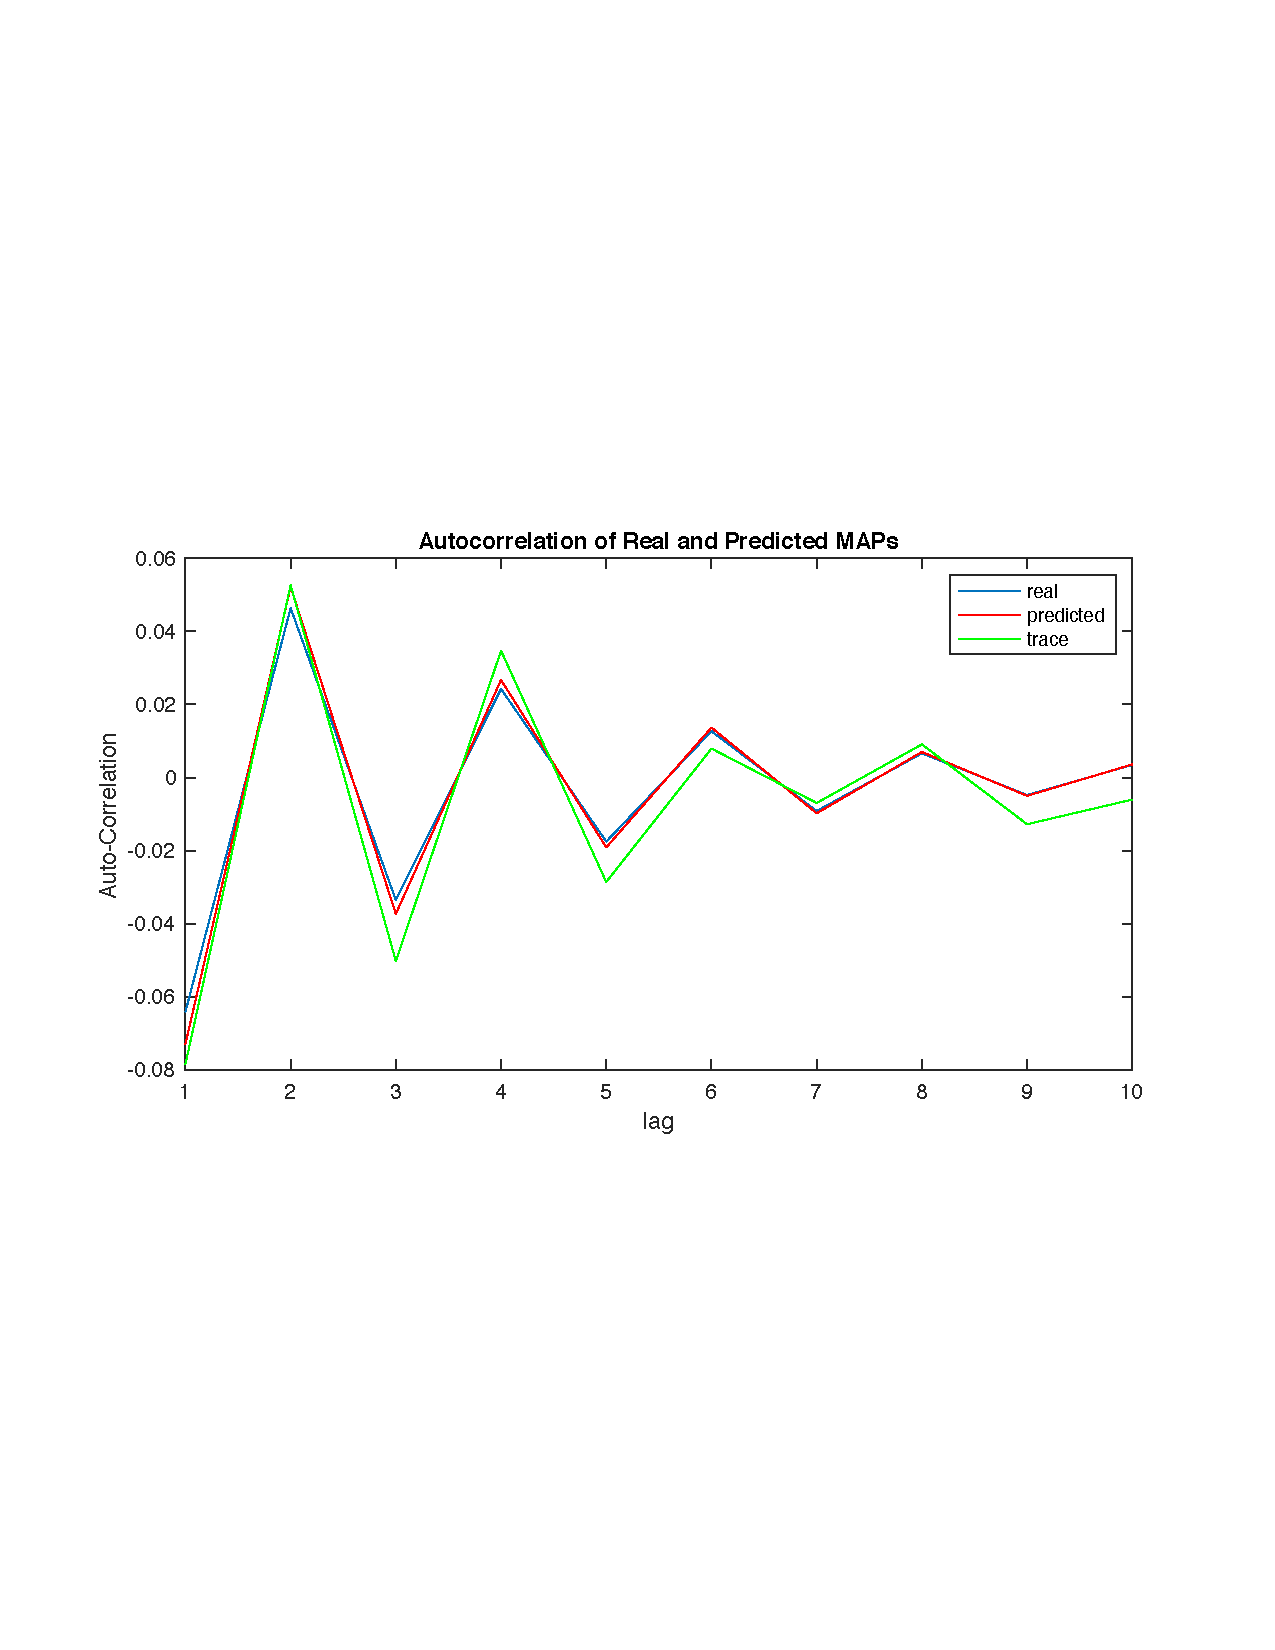
\includegraphics[width=100mm, scale=0.5]{mm1_ac.pdf}
\caption{Auto-correlation of Real and Predicted MAPs for M/M/1 Example}
\label{fig:mm1_ac}
\end{center}
\end{figure}

\subsection{EM Algorithm Example: MAP built from M/G/1 Network}

We will now consider how well our algorithm fits to a slightly more challenging example. We assume that there is one class of incoming jobs with non-exponential service times. We make the service times Erlang distributed with unit rate and variance 1/3. We then build an MAP from this queueing network by using the matrix:

\begin{equation}
    \mathbf{D}_1 = \begin{bmatrix}
     0 &   0  &  0  &  0.10 \\
     2.0  &  0.50  &  0  &  0 \\
     0 & 1.00 & 2.00 & 0 \\
     0 & 0 & 1.00 & 0.50
    \end{bmatrix}
\end{equation}

From the M/G/1 queueing network, the generator matrix for the underlying Markov chain is shown in Equation \ref{eqn:gen_mg1}:

\begin{equation}
    \mathbf{Q} = \begin{bmatrix}
-0.50    &     0    &     0  &  0.50 \\
3.00  & -3.00   &      0    &     0 \\
0  &  3.00  & -3.00   &     0 \\
0    &     0  &  3.00  & -3.00 \\
    \end{bmatrix}
    \label{eqn:gen_mg1}
\end{equation}

therefore, the matrix $\mathbf{D}_0$ becomes: 

\begin{equation}
    \mathbf{D}_0 = \begin{bmatrix}
-0.50    &     0     &    0   & 0.40 \\
1.00 &  -3.50  &      0    &     0 \\
0  &  2.00 &  -5.00    &     0 \\
0    &     0   & 2.00 &  -3.50
    \end{bmatrix}
\end{equation} \\

\textbf{Evaluation of EM Algorithm for M/G/1 Example}: For this example we used 1000 samples in the trace that we generate from the real MAP using the matrices shown above. We have that the matrices in our predicted MAP are as follows: 

\begin{equation}
    \mathbf{D}_{0p} = \begin{bmatrix}
-0.4266    &     0   &      0    &     0 \\
0  & -0.5045 &       0    &     0 \\
0  &  0 &  -2.5920    &     0 \\
0    &  0  &  0 &  -4.1088
    \end{bmatrix}
\end{equation} \\

\begin{equation}
    \mathbf{D}_{1p} = \begin{bmatrix}
    0.0550  &  0.0797  &  0.1335  &  0.1583 \\
    0.0983  &  0.0919  &  0.1632  &  0.1510 \\
    1.8623  &  0.6087  &  0.1131  &  0.0080 \\
    0.1800  &  0.0912  &  2.3648  &  1.4729
    \end{bmatrix}
\end{equation} \\

therefore, we notice in our predicted matrix $\mathbf{D}_{1p}$ that we have non-zero values in places that in our generating matrix $\mathbf{D}_1$ we have zero values. Let us see if this affects our prediction of the metrics auto-correlation, mean and variance. Table \ref{tab:mg1_mean_var} shows the mean and variance of the real and predicted matrices. We have that our predicted MAP predicts the mean and variance to a very high accuracy. \\ 

\begin{table}[h!]
\begin{center}
\begin{tabular}{|l|l|l|}
\hline
M/G/1 & Mean & Variance \\ \hline
Real MAP & 1.184 & 3.137 \\ \hline
Predicted MAP & 1.183 & 3.213 \\ \hline
\end{tabular}
\caption{}
\label{tab:mg1_mean_var}
\end{center}
\end{table}

Figure \ref{fig:mg1_ac} shows the auto-correlation of the real MAP, predicted MAP and the trace. We have that the pattern of the predicted auto-correlation matches that of the real auto-correlation very well, which suggests that our EM algorithm has predicted the parameters of the real MAP well. Therefore, even though our predicted matrix is not able to predict accurately the location of non-zero values, the metrics of prediction still have high quality. hence, we can conclude that our EM algorithm works well for this more complex problem. 

\begin{figure}[h!]
\begin{center}
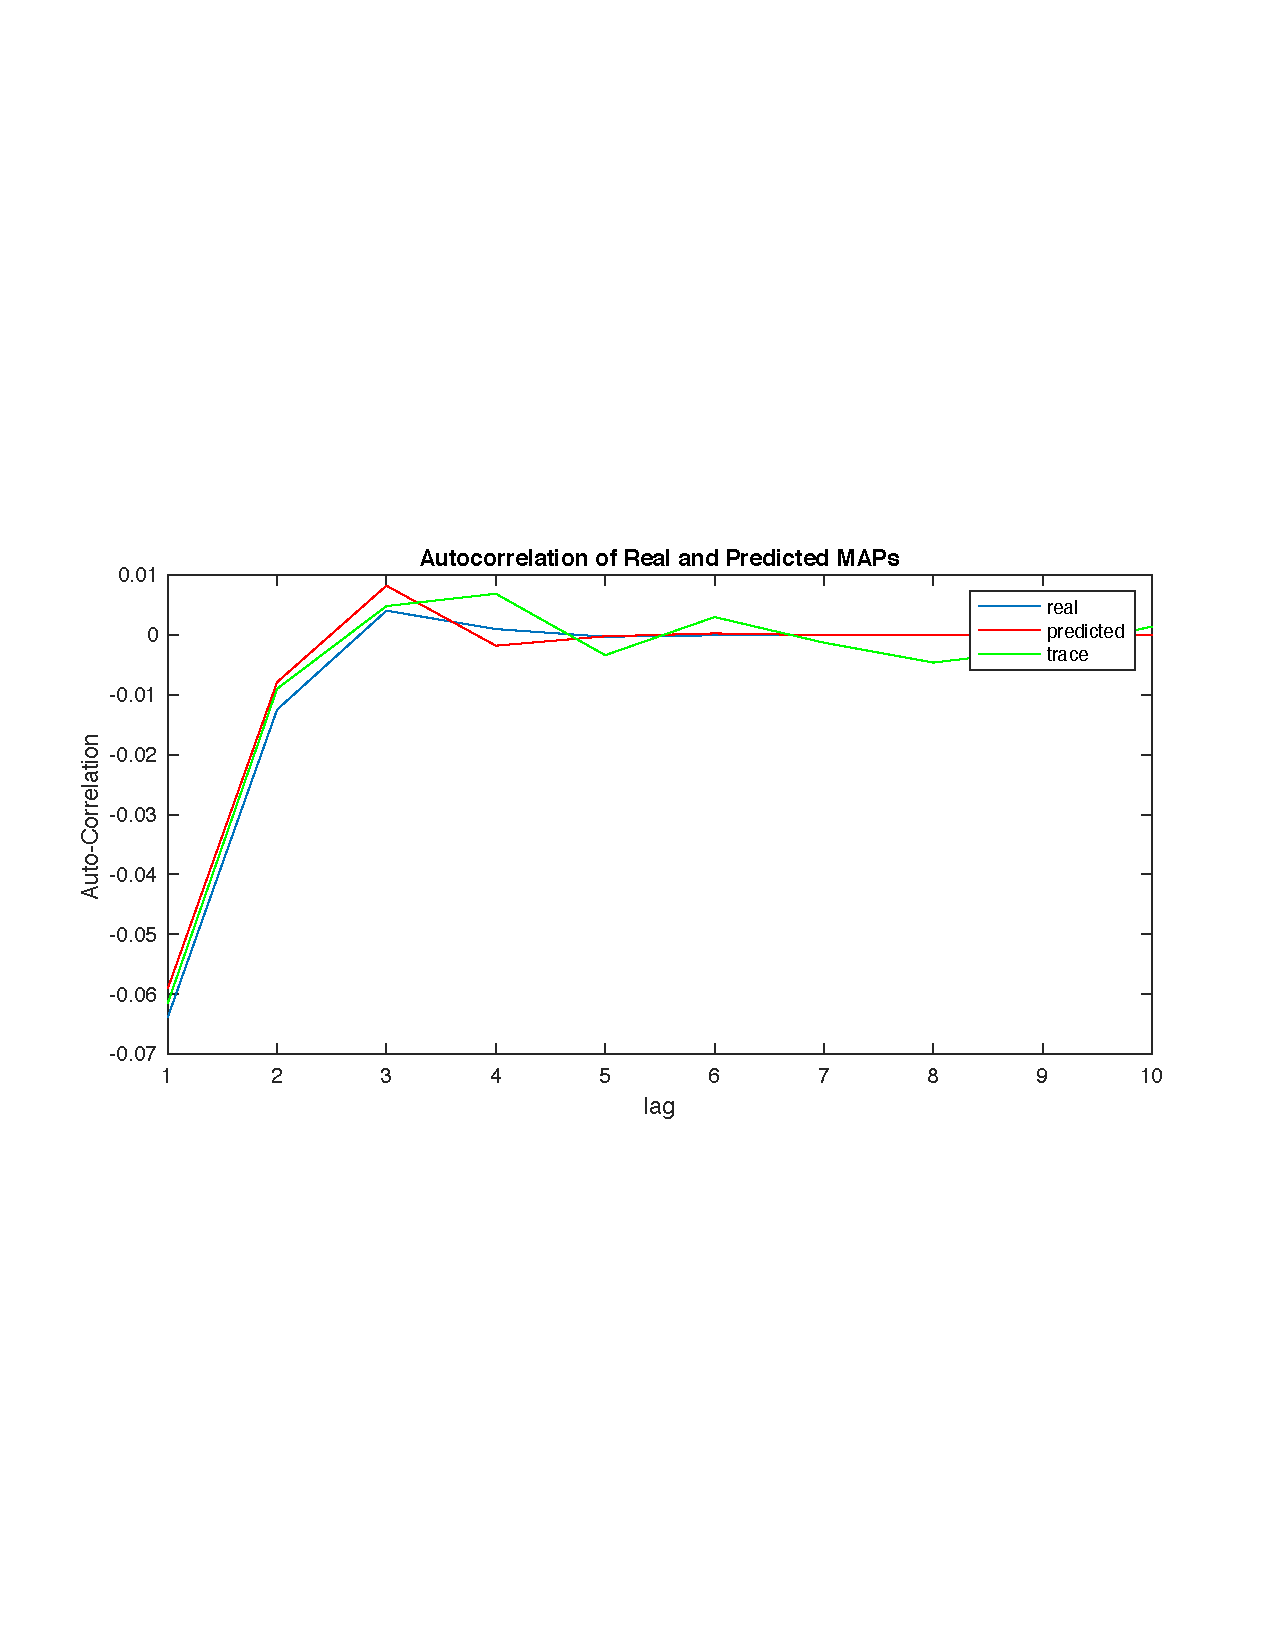
\includegraphics[width=100mm, scale=0.5]{mg1_ac.pdf}
\caption{Auto-correlation of Real and Predicted MAPs for M/G/1 Example}
\label{fig:mg1_ac}
\end{center}
\end{figure}

\subsection{EM Algorithm Example: MAPs built from Machine Repairman Models}

For these next few examples, we will aim to replicate and predict the parameters of MAPs that are built from queueing networks that are created using machine repairman models. This section is important as we want to see how well our algorithm can predict parameters of MAPs even when the MAP is very complicated. An example of a machine repairman model was shown in Figure \ref{fig:machinerepairmanmodel}. A machine repairman model is a closed model where jobs perpetually cycle within a network of queues [Bol06]. In this situation, we consider a group of repairmen who are tasked with fixing machines as they break. In the model, we define the number of repairmen, denoted as $S$, and the total number of machines, denoted by $N$. We define the rate at which machines break down, and subsequently define an exponential distribution which determines the rate at which a machine gets fixed. The total number of machines are placed in `delay' nodes within the queuing network, and the number of repairmen are placed in `queue' nodes.

\subsubsection{Example 1}

In this example we consider a machine repairman model with $S = 2$ and $N=2$. The rate at which machines break down is defined by $\mu_n = 0.5$ and the rate machines get fixed is set as $\mu_s = 2$. We then use a SolverCTMC method, as defined in LINE [Lin20] to find the generator matrix for this model, denoted by $\mathbf{Q}$. In this example we have that:

\begin{equation}
    \mathbf{Q} = 
\begin{bmatrix}
-4.0 & 4.0 & 0\\
0.5 & -2.5 & 2.0\\
0 & 1.0 & -1.0
\end{bmatrix}
\end{equation} \\

We use this generator matrix to build the MAP that we subsequently use to sample a trace of inter-arrival times. We then input the sampled trace into our EM algorithm which attempts to predict the parameters of the underlying MAP. To build an MAP from this model we define a $3 \times 3$ matrix denoted as $\mathbf{D}_1$, and then using this matrix and the matrix $\mathbf{Q}$ we can define the matrix $\mathbf{D}_0$ as:

\begin{equation}
    \mathbf{D}_0 = \mathbf{Q} - \mathbf{D}_1.
\end{equation}

In this example, we have set:

\begin{equation}
    \mathbf{D}_1 = 
\begin{bmatrix}
0.200 & 3.00 & 0.001\\
1.00 & 0.100 & 0.001\\
0.005 & 0.003 & 0.020
\end{bmatrix}
\end{equation}

such that $\mathbf{D}_0$ becomes: 

\begin{equation}
    \mathbf{D}_0 = 
\begin{bmatrix}
-4.200 & 1.00 & -0.001\\
-0.500 & -2.600 & 1.999\\
-0.005 & 0.9970 & -1.020
\end{bmatrix}
\end{equation} \\

We then use the `map\_normalize' method in LINE, which aims to make certain that our underlying MAP has all the proper characteristics of an MAP. This function creates an MAP from two input matrices $\mathbf{D}_0$ and $\mathbf{D}_1$ such that `$\mathbf{D}_0$ is normalized to make $\mathbf{D}_0+ \mathbf{D}_1$ an infinitesimal generator, with all negative entries set to zero, and with complex values set equal to their norm' [Lin20] After normalization, we have the following matrices for the MAP $M = \{\mathbf{D}_0, \mathbf{D}_1\}$ that we will draw a sample trace from:

\begin{equation}
    \mathbf{D}_0 = 
\begin{bmatrix}
-4.201 & 1.00 & 0\\
0 & -3.100 & 1.999\\
0 & 0.9970 & -1.0250
\end{bmatrix}
\end{equation} \\

\begin{equation}
    \mathbf{D}_1 = 
\begin{bmatrix}
0.200 & 3.00 & 0.001\\
1.00 & 0.100 & 0.001\\
0.005 & 0.003 & 0.020
\end{bmatrix}
\end{equation} \\

\textbf{Process of Predicting Parameters from a Trace for Ex. 1}: Now that we have built our generator MAP, we can use it to sample a trace. Because our generator matrices are not so large in size, we will start with only using a trace of 1000 samples. In general, the higher number of samples we have in the trace the longer the algorithm takes to run. We then use our EM algorithm on the trace, where the expectation part is detailed in Section 4.5 and the maximisation part is detailed in Section 4.4. We set the maximum number of iterations of the algorithm to be 300, the stopping condition to be when the change in the log likelihood is less than $1e^{-7}$, and we use random initial conditions. \\

\textbf{Evaluation of our Algorithm Ex. 1}: Firstly, we will look at the predicted matrices $\mathbf{D}_{0p}$ and $\mathbf{D}_{1p}$ that define the predicted MAP $M_{p} = \{\mathbf{D}_{0p},\mathbf{D}_{1p}\}$. In this example, out algorithm has predicted these matrices to be: 

\begin{equation}
    \mathbf{D}_{0p} = 
\begin{bmatrix}
-0.3139 & 0 & 0\\
0 & -3.1438 & 0\\
0 & 0 & -3.977
\end{bmatrix}
\end{equation} \\

\begin{equation}
    \mathbf{D}_{1p} = 
\begin{bmatrix}
0.088 & 0.0254 & 0.2005\\
0.4218 & 0.0549 & 2.6671\\
2.9841 & 0.7220 & 0.2709
\end{bmatrix}
\end{equation} \\

Table \ref{table:ex1_mean_var} shows the mean and variance for the real MAP and the predicted MAP. We can see that our predicted MAP matches both the mean and the variance very well, with only a slight discrepancy between the values. 

\begin{table}[h!]
\begin{center}
\begin{tabular}{|l|l|l|}
\hline
Example 1 & Mean & Variance \\ \hline
Real MAP & 1.6505 & 7.0998 \\ \hline
Predicted MAP & 1.6141 & 6.8435 \\ \hline
\end{tabular}
\caption{}
\label{table:ex1_mean_var}
\end{center}
\end{table}

Figure \ref{fig:mr_2_2_ac} shows the auto-correlation of lag for values $k$ up to 10. From the figure, we can see that our predicted MAP matches the auto-correlation of the MAP almost perfectly, which suggests that our algorithm has managed to predict the behaviour and parameters of the original MAP very well. 

\begin{figure}[h!]
\begin{center}
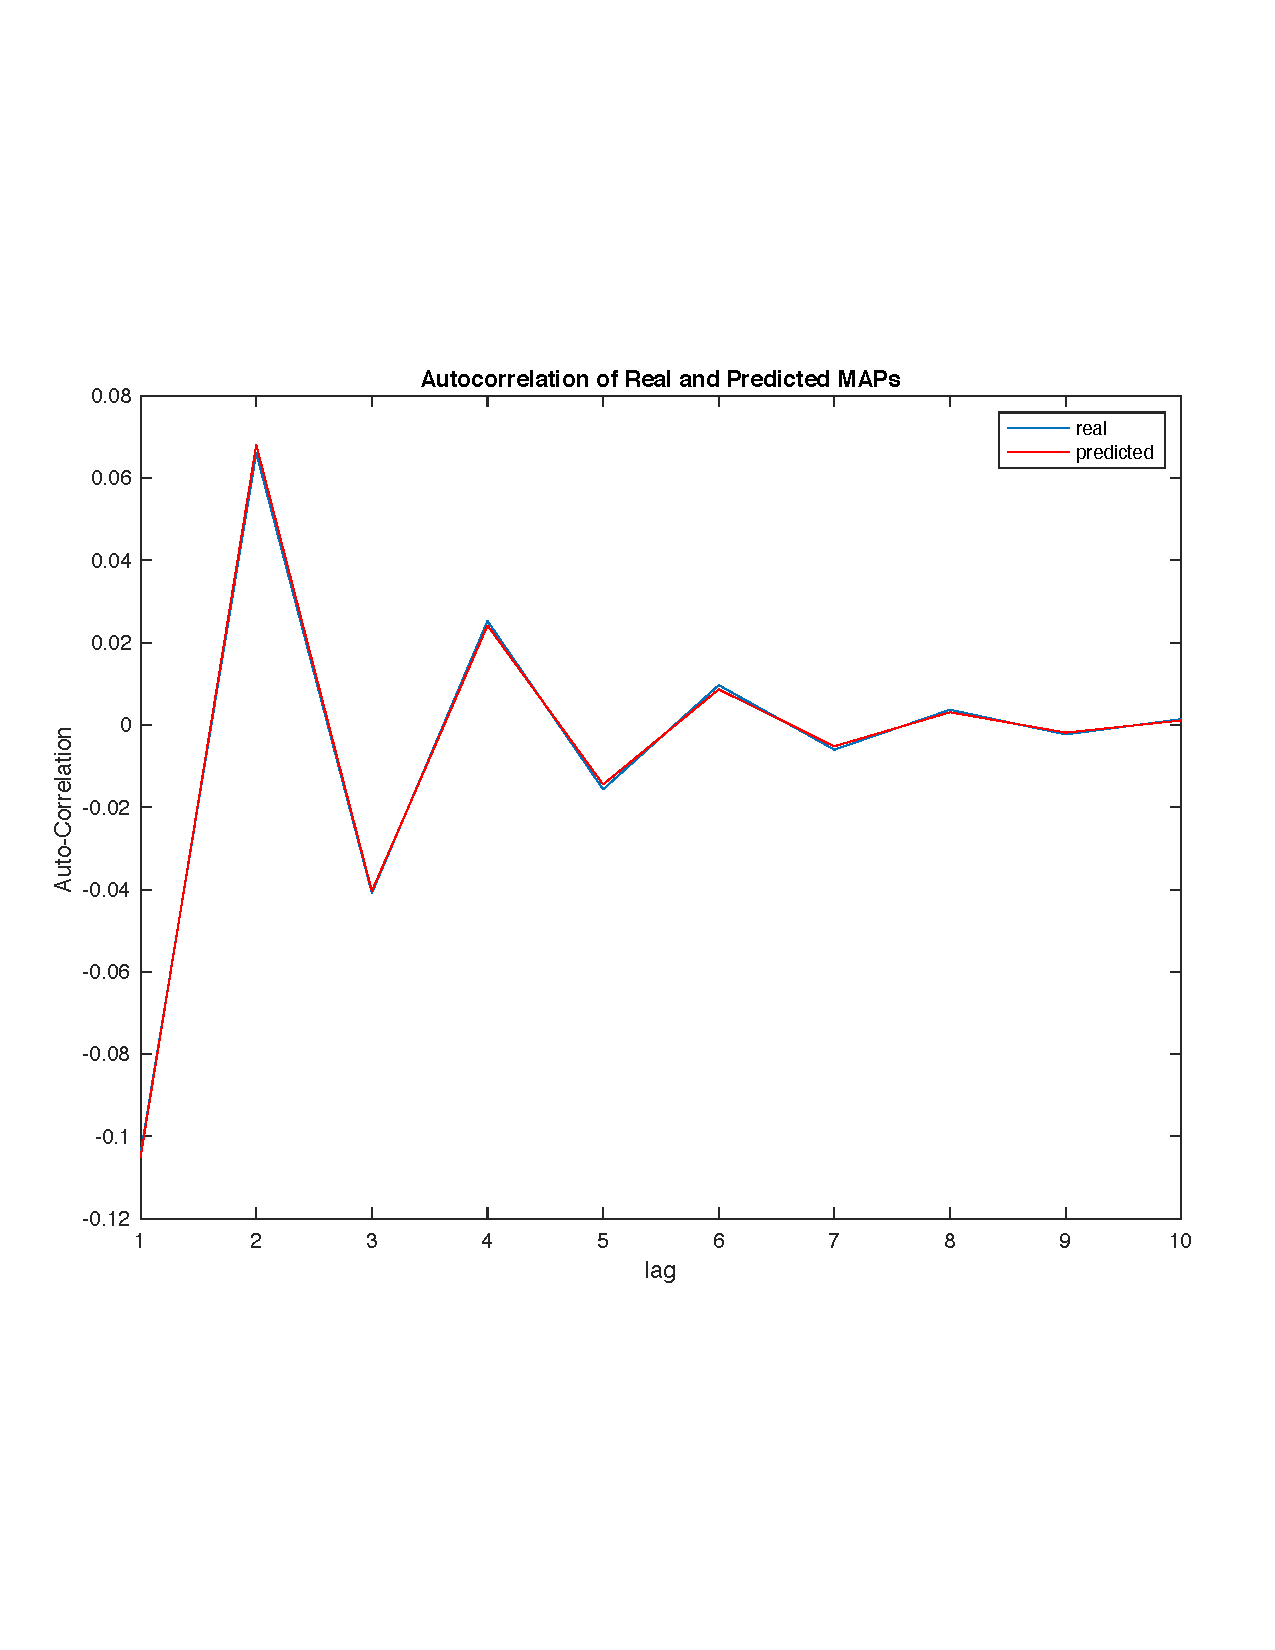
\includegraphics[width=100mm, scale=0.5]{mr_2_2_ac.pdf}
\caption{Auto-correlation of Real and Predicted MAPs for Example 1}
\label{fig:mr_2_2_ac}
\end{center}
\end{figure}

\subsubsection{Example 2}

As in Example 1, we will consider a machine repairman model. We will use the following values in our generating MAP: $N=3$, $S=3$. The building process is very similar to Example 1, therefore we will only show the matrices $\mathbf{D}_0$ and $\mathbf{D}_1$ after normalization. The generating matrices for this example are shown in Equations \ref{eqn:ex_2_D0} - \ref{eqn:ex_2_D1}: 
    
\begin{equation}
  \mathbf{D}_0 = \begin{bmatrix}
 -7.2410  &  5.5000  &  0  &    0 \\
0.4000  & -6.5060  &  3.9950  & 0 \\
0   & 0.9980 &  -3.0320  &  1.8000 \\
0   &  0  &  0.5000 &  -4.0000 
    \end{bmatrix}
    \label{eqn:ex_2_D0}
\end{equation} \\
    
\begin{equation}
  \mathbf{D}_1 = \begin{bmatrix}
 0.7210  &  0.5000  &  0.0200  &  0.5000 \\
    0.1000  &  1.2060   & 0.0050  &  0.8000 \\
    0.0010   & 0.0020  &  0.0310  &  0.2000 \\
    0.1000  &  0.4000  &  1.0000  &  2.0000
    \end{bmatrix}
    \label{eqn:ex_2_D1}
\end{equation} \\

\textbf{Process of Predicting Parameters from a Trace for Ex. 2}: We have that the process to predict the MAP parameters is similar to that of Example 1, where we sample a trace from the generating MAP and pass it through our EM algorithm. We used 1000 samples in the trace for this example. We used a maximum iteration size of 300. \\

\textbf{Evaluation of EM algorithm on Ex. 2}: After running our algorithm to give us a predicted MAP based on the trace, we have that the MAP consists of the following matrices shown in Equations \ref{eqn:ex_2_D0p} - \ref{eqn:ex_2_D1p}:

\begin{equation}
  \mathbf{D}_0 = \begin{bmatrix}
-1.6903    &     0     &    0    &     0 \\
0  & -1.7060    &     0     &    0 \\
0     &    0 &  -1.8086    &     0 \\
0    &     0    &     0  & -5.3934
    \end{bmatrix}
    \label{eqn:ex_2_D0p}
\end{equation} \\
    
\begin{equation}
  \mathbf{D}_1 = \begin{bmatrix}
    0.4711  &  0.4758 &   0.4136  &  0.3298 \\
    0.4774  &  0.4814  &  0.4171  &  0.3301 \\
    0.5101  &  0.5137  &  0.4429  &  0.3420 \\
    1.5467  &  1.5574  &  1.3388  &  0.9505
    \end{bmatrix}
    \label{eqn:ex_2_D1p}
\end{equation} \\

Figure \ref{fig:mr_3_3_ac} shows the auto-correlation of lag for the real and predicted MAPs, as well as the trace that is sampled from the real MAP. We see that for this MAP our algorithm is slightly worse at predicting the auto-correlation of lag than in Example 1. We have that the prediction for the mean and the variance is very good, as shown in Table \ref{table:ex2_mean_var}. \\

\begin{table}[h!]
\begin{center}
\begin{tabular}{|l|l|l|}
\hline
Example 2 & Mean & Variance \\ \hline
Real MAP & 0.5032 & 0.3002 \\ \hline
Predicted MAP & 0.5036 & 0.3014 \\ \hline
\end{tabular}
\caption{Accuracy of Predicted Mean and Variance of MAPs for Example 2}
\label{table:ex2_mean_var}
\end{center}
\end{table}

\begin{figure}[h!]
\begin{center}
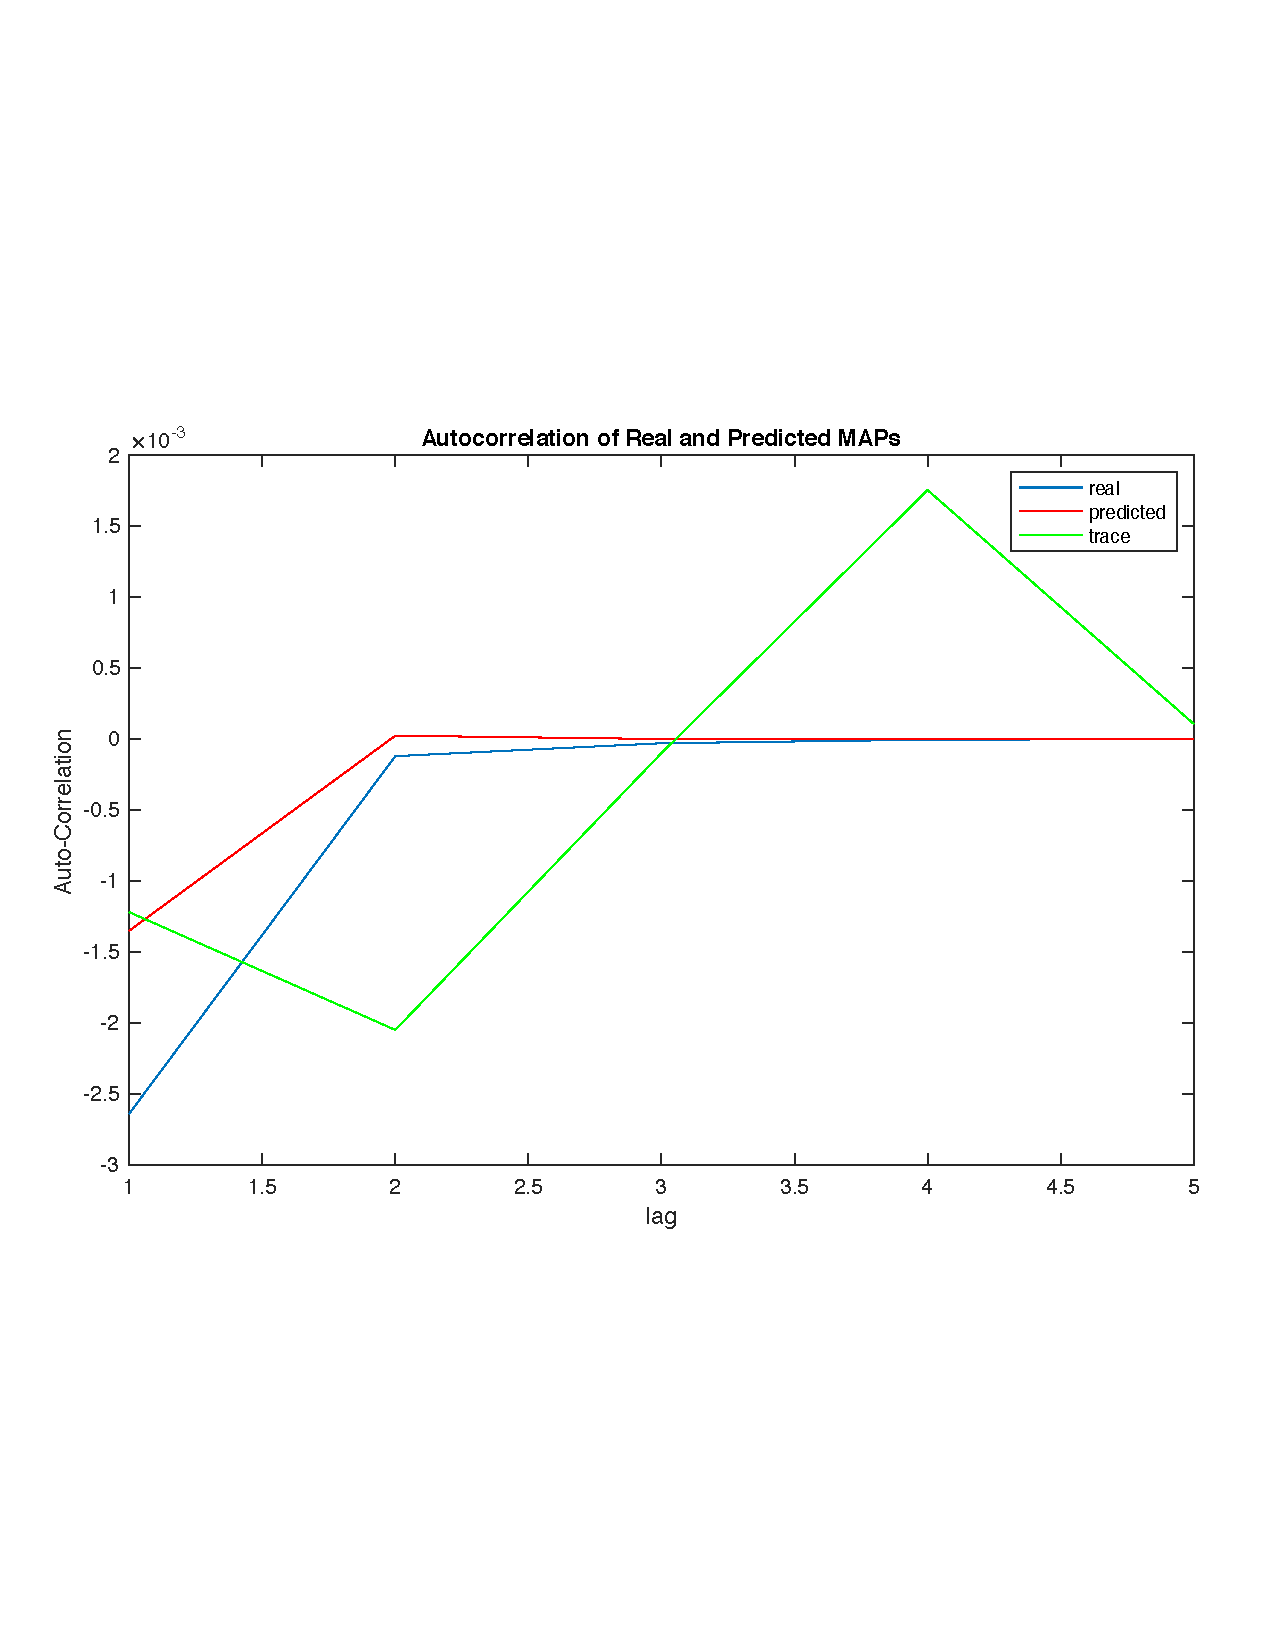
\includegraphics[width=100mm, scale=0.5]{mr_3_3_ac.pdf}
\caption{Auto-correlation of Real and Predicted MAPs for Example 2}
\label{fig:mr_3_3_ac}
\end{center}
\end{figure}

As we have that the auto-correlation of the real MAP is not predicted very well by our fitted MAP, we have included another metric which is the distribution of our real MAP, predicted MAP and the trace. Figure \ref{fig:mr_3_3_cdf} shows the distribution of each plotted against time. We have that the distribution is predicted almost perfectly using our predicted MAP. This suggests that we have fit the parameters very well in our prediction. The 'red' line shows the distribution of the predicted MAP, where we have that the distribution of the predicted MAP is so close to that of the trace and the real MAP that we in fact can hardly see the red line. However, it is there, it is just perfectly situated on the green and blue lines. 


\begin{figure}[h!]
\begin{center}
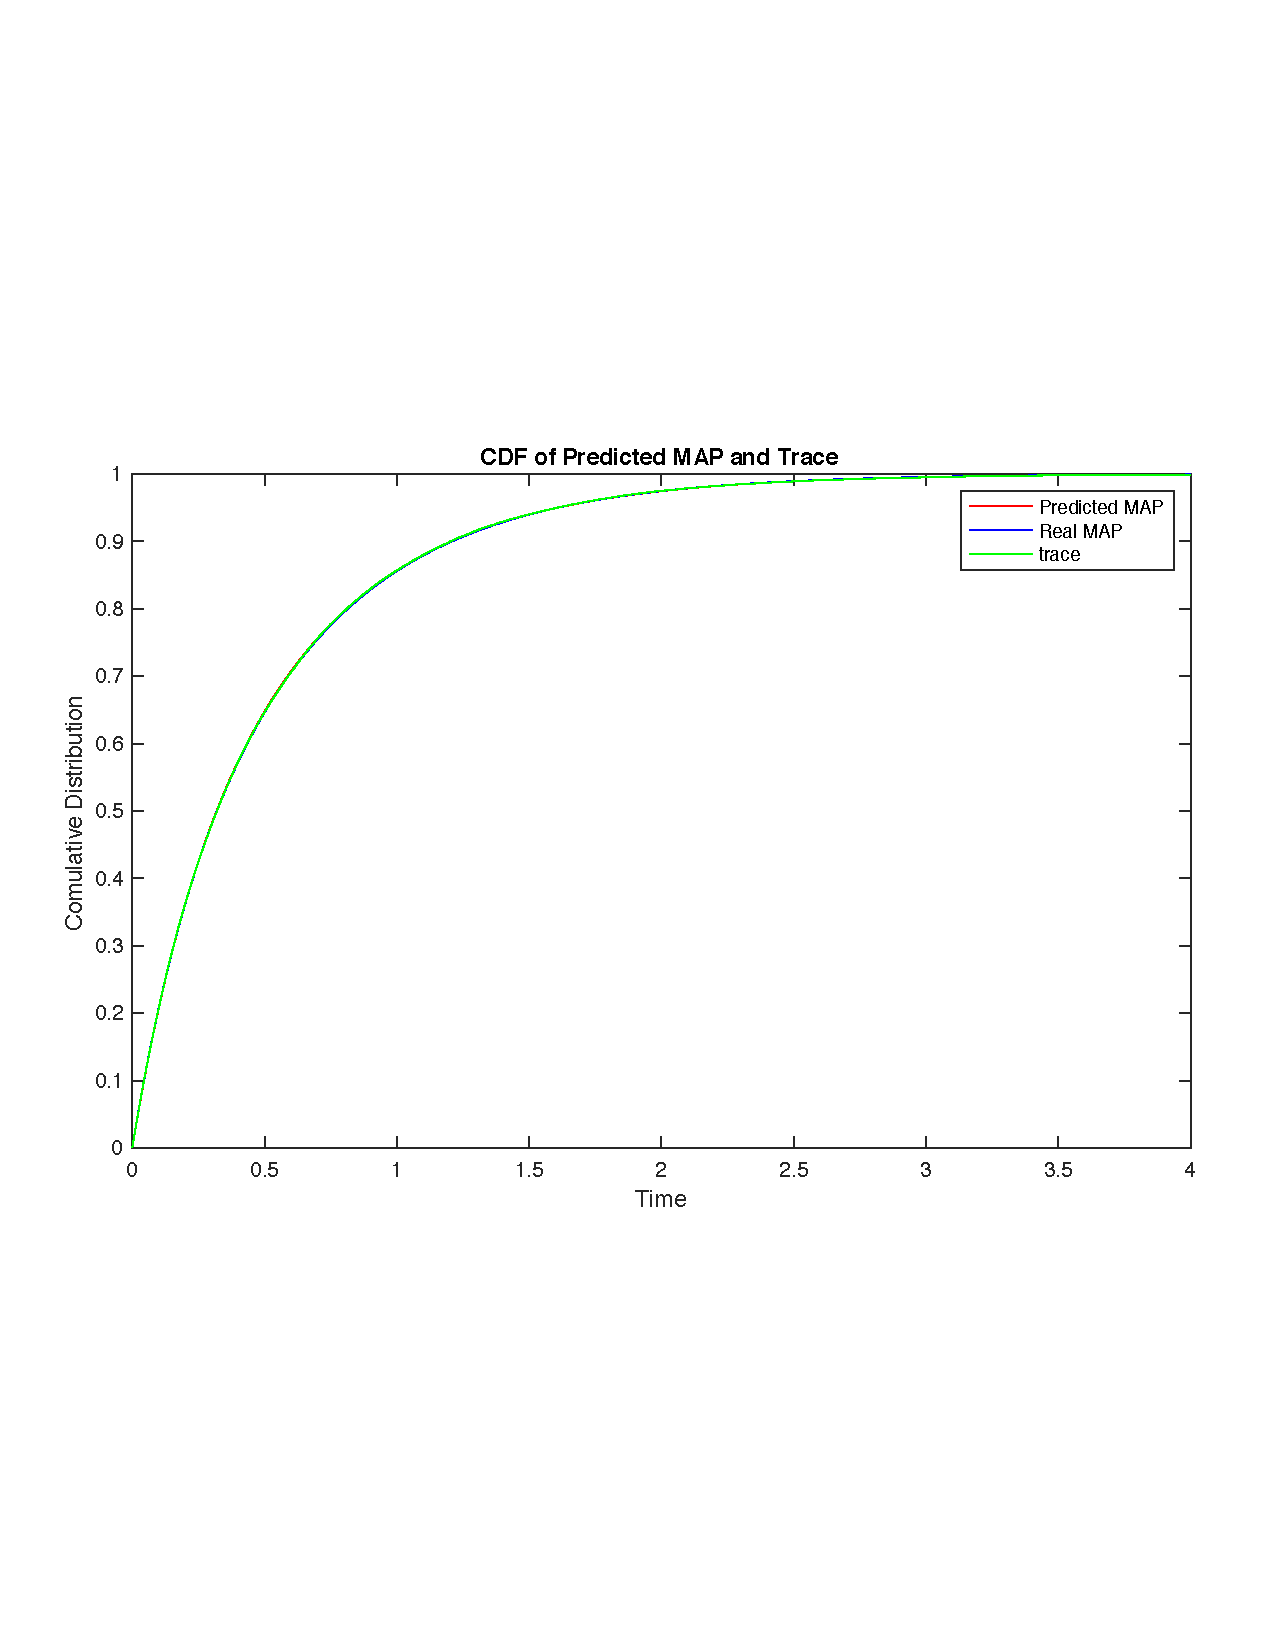
\includegraphics[width=100mm, scale=0.5]{mip_3_3_cdf.pdf}
\caption{Distribution of Real and Predicted MAPs for Example 2}
\label{fig:mr_3_3_cdf}
\end{center}
\end{figure}

\subsubsection{Example 3}

As in Example 1 and 2, we will consider a machine repairman model. This time however, we will use even larger values of $N$ and $S$ to see how well our algorithm fits to more complex MAPs. We will use the following values in our generating MAP: $N=5$, $S=3$. The building process is very similar to Example 1, therefore we can skip some steps and only discuss the matrices $\mathbf{D}_0$ and $\mathbf{D}_1$ after normalization. The generating matrices for this example are shown in Equations \ref{eqn:ex_3_D0} - \ref{eqn:ex_3_D1}: 

\begin{equation}
    \mathbf{D}_{0} = 
\begin{bmatrix}
-7.240 & 5.50 & 0 & 0 & 0 & 0\\
0 & -8.00 & 5.50 & 0 & 0 & 0\\
0 & 0 & -7.50 & 4.50 & 0 & 0\\
0 & 0 & 1.40 & -9.10 & 3.50 & 0\\
0 & 0 & 0 & 1.90 & -4.90 & 1.99\\
0 & 0 & 0 & 0 & 2.490 & -5.410
\end{bmatrix}
\label{eqn:ex_3_D0}
\end{equation} \\


\begin{equation}
    \mathbf{D}_{1} = 
\begin{bmatrix}
1.0000  &  0.5000  &  0.2000  &  0.0100  &  0.0100 & 0.0200\\
0.5000  &  1.0000 &   0.5000  &  0.2000  &  0.1000 & 0.2000\\
0.1000  &  1.0000  &  0.2000  &  1.5000  &  0.1000 & 0.1000\\
0.5000 &   1.0000  &  0.1000 &   2.0000 &   0.5000 & 0.1000\\
0.1000  &  0.1000  &  0.2000  &  0.1000  &  0.5000 & 0.0100\\
0.4000 &   0.0100   & 0.7000  &  0.8000 &   0.0100& 1.0000
\end{bmatrix}
\label{eqn:ex_3_D1}
\end{equation}  \\

\textbf{Process to Predict Parameters from a Trace for Ex. 3}: We have that the process to predict the MAP parameters is similar to that of Example 1, where we sample a trace from the generating MAP and pass it through our EM algorithm. We used 10000 samples in the trace for this example, as we had a much larger state size. Additionally, we used a maximum iteration size of 400 instead of 300. \\

\textbf{Evaluation of EM algorithm Ex. 3}: This example is the most challenging that we have had so far, as we have a far bigger state space and a more complex machine repairman model from which we built the generating MAP. Our predicted MAP has the following matrices, shown in Equations \ref{eqn:ex_3_D0p} - \ref{eqn:ex_3_D1p}:

\begin{equation}
    \mathbf{D}_{0} = 
\begin{bmatrix}
-2.109 & 0 & 0 & 0 & 0 & 0\\
0 & -2.1367 & 0 & 0 & 0 & 0\\
0 & 0 & -2.2041 & 0 & 0 & 0\\
0 & 0 & 0 & -2.438 & 0 & 0\\
0 & 0 & 0 & 0 & -3.3441 & 0\\
0 & 0 & 0 & 0 & 0 & -5.7501
\end{bmatrix}
\label{eqn:ex_3_D0p}
\end{equation} \\

\begin{equation}
    \mathbf{D}_{1} = 
\begin{bmatrix}
 0.4040  &  0.4345  &  0.3963  &  0.3382  &  0.2795  &  0.2565\\
0.4024  &  0.4362  &  0.4008  &  0.3448  &  0.2874  &  0.2651\\
0.4048  &  0.4428  &  0.4113  &  0.3586  &  0.3037  &  0.2830\\
0.4279  &  0.4736  &  0.4471  &  0.3999  &  0.3504  &  0.3339\\
0.5460  &  0.6131  &  0.5929  &  0.5546  &  0.5201  &  0.5174\\
0.8721  &  0.9919  &  0.9809  &  0.9586  &  0.9617  &  0.9850
\end{bmatrix}
\label{eqn:ex_3_D1p}
\end{equation}  \\

Figure \ref{fig:mr_5_3_ac} shows the auto-correlation of lag for the predicted and real MAPs, as well as the auto-correlation of lag for the sample trace from the real MAP. As can be seen in the figure, we have that the prediction of the auto-correlation is much worse than that of Example 1. We used 10000 samples from the real MAP, which is perhaps not enough for an MAP of this complexity. The auto-correlation of lag for the trace shows the complexity of the sample we have taken, and our predicted MAP struggled to accurately predict it. The overall pattern is similar however, so we can conclude that our method of prediction is along the right lines. Additionally, as can be seen in Table \ref{table:ex3_mean_var} the mean and the variance of the MAP is predicted almost perfectly. \\

\begin{table}[h!]
\begin{center}
\begin{tabular}{|l|l|l|}
\hline
Example 3 & Mean & Variance \\ \hline
Real MAP & 0.3919 & 0.1758 \\ \hline
Predicted MAP & 0.3924 & 0.1757 \\ \hline
\end{tabular}
\caption{Accuracy of Predicted Mean and Variance of MAPs for Example 3}
\label{table:ex3_mean_var}
\end{center}
\end{table}

\begin{figure}[h!]
\begin{center}
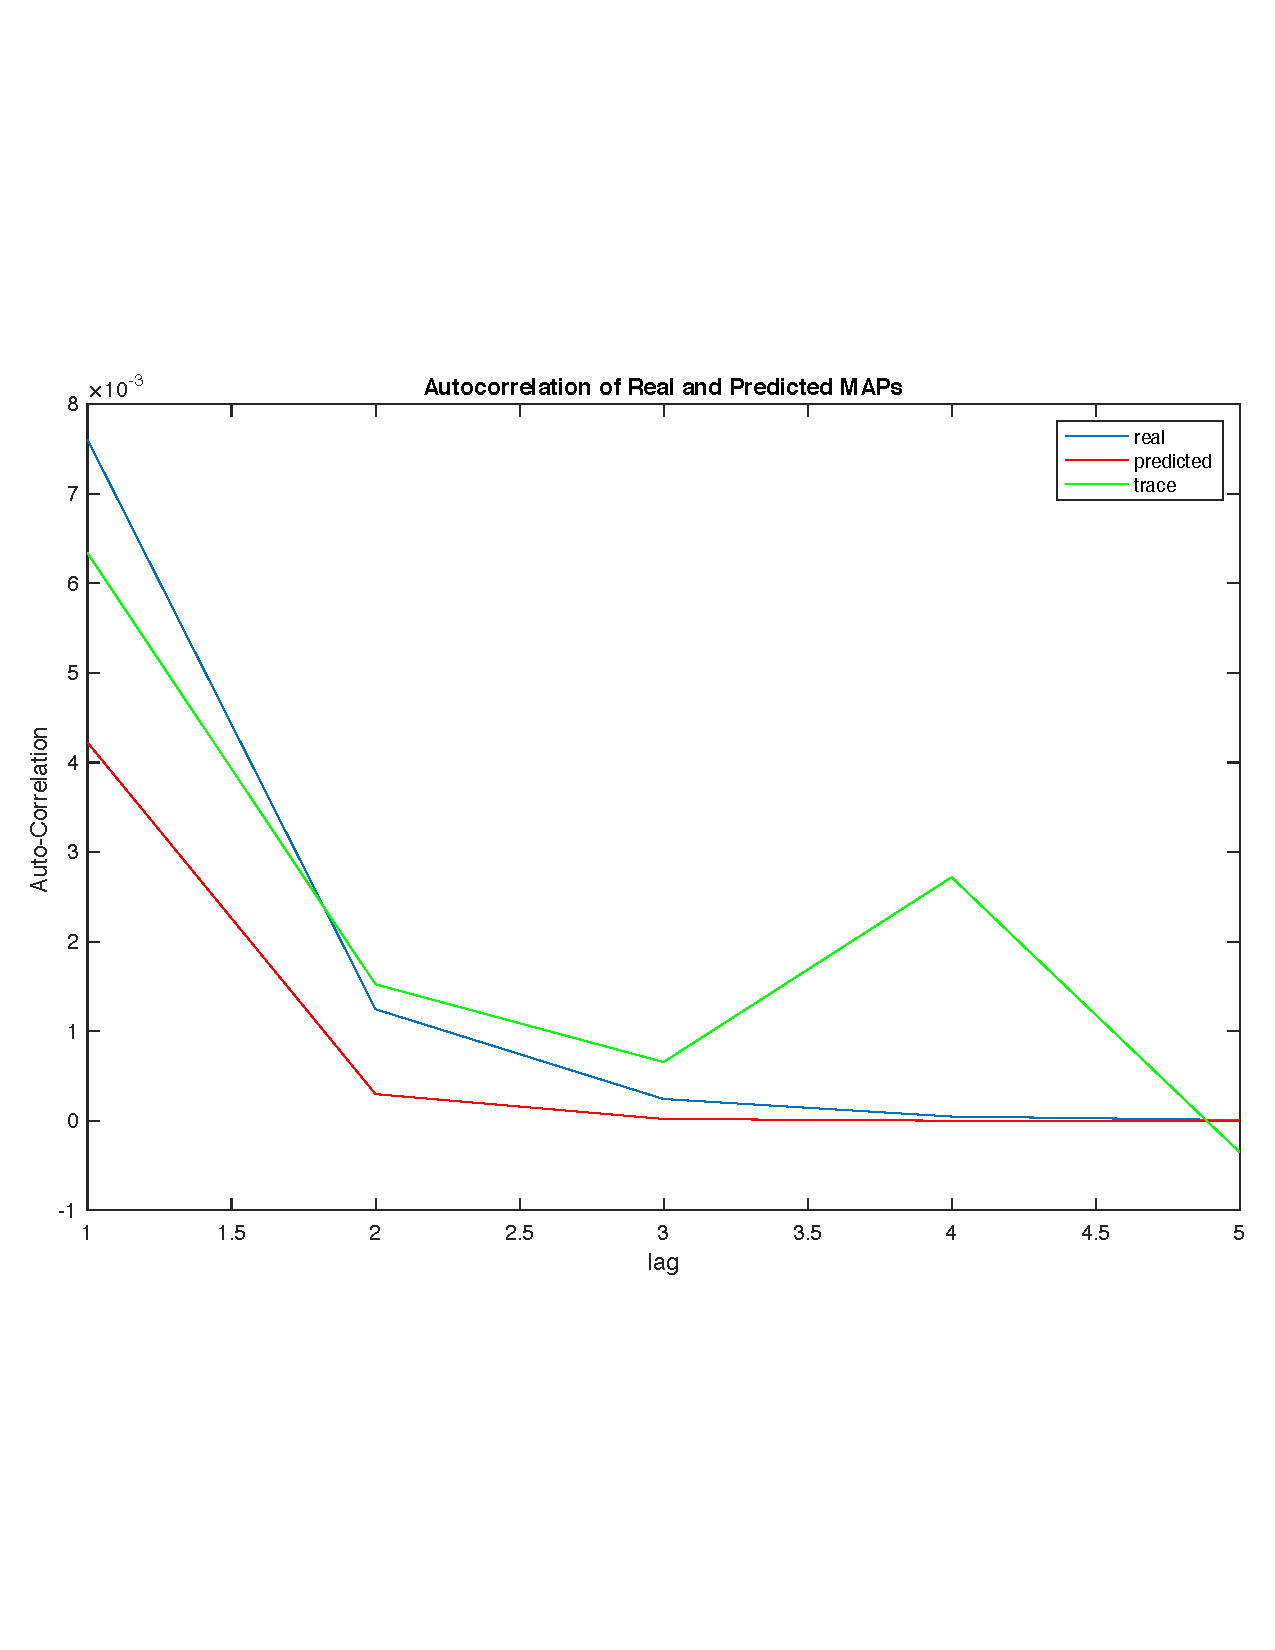
\includegraphics[width=100mm, scale=0.5]{mr_5_3_ac.pdf}
\caption{Auto-correlation of Real and Predicted MAPs for Example 3}
\label{fig:mr_5_3_ac}
\end{center}
\end{figure}

As the predicted auto-correlation is not a great fit, we will also consider the distribution of the predicted MAP, the real MAP, and the trace to get an idea of how well we predict the parameters. Figure \ref{fig:mr_5_3_cdf} shows the distribution functions of the MAPs and the trace. As we can see from the figure, it is hard to distinguish between the three, which suggests that we have predicted the parameters very well. 

\begin{figure}[h!]
\begin{center}
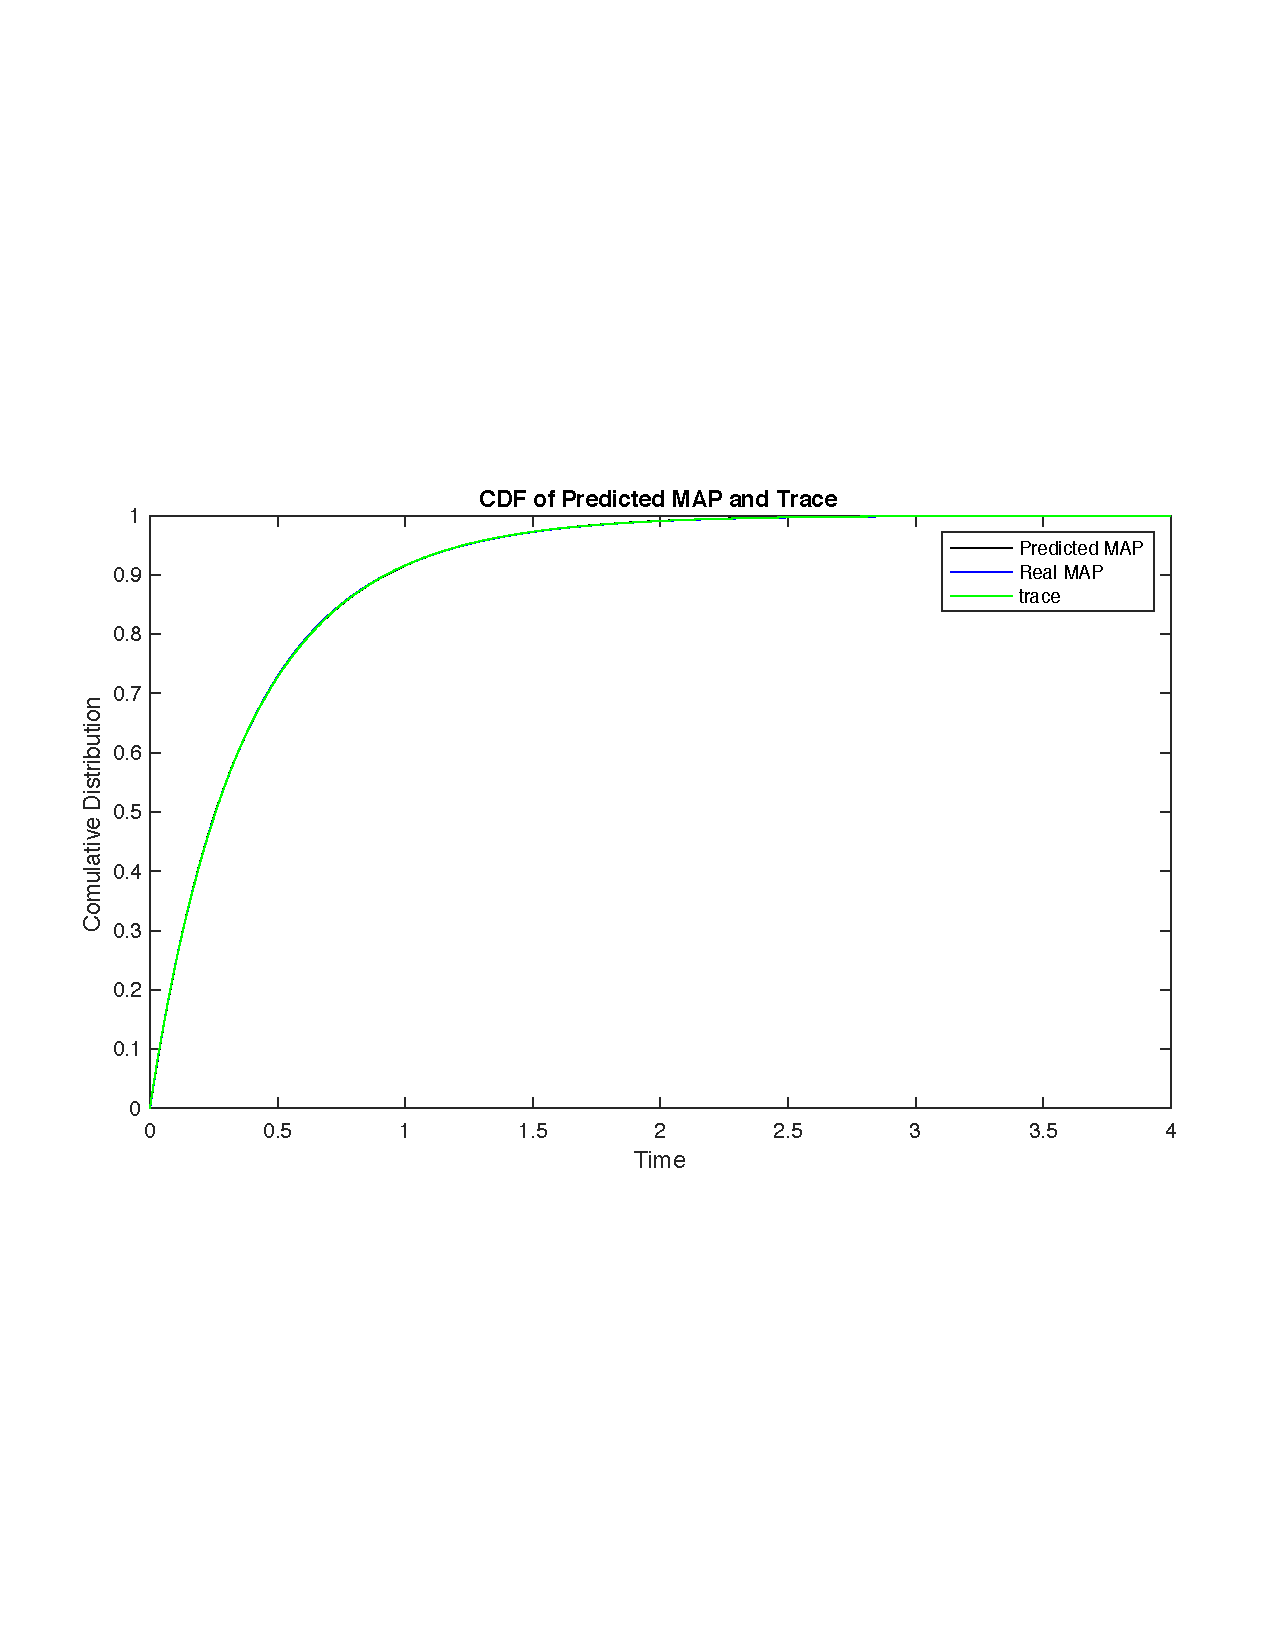
\includegraphics[width=100mm, scale=0.5]{mip_5_3_cdf.pdf}
\caption{CDF of Real and Predicted MAPs for Example 3}
\label{fig:mr_5_3_cdf}
\end{center}
\end{figure}

\subsection{Fitting MAPs to Real Trace Data}

We will now see how well our EM algorithm fits to real trace data. We will use two examples of real traces of inter-arrival times, taken from the Internet Traffic Archive [ITA], and then evaluate the accuracy and quality of our EM algorithm to be able to generate similar traces. 

\subsubsection{Example of a Real Trace Measured from LAN Traffic}

In this example we will use the `BCAUG89' trace which was measured from LAN traffic. This trace contains `a million packet arrivals seen on an Ethernet at the Bellcore Morristown Research and Engineering facility [ITA]'. The tracing was performed at the Bellcore Morristown Research and Engineering facility, on the computing lab's Ethernet, which carried `primarily local traffic, but also all traffic between Bellcore and the Internet' [ITA]. The timestamps have 4-microsecond precision, and when undergoing further analysis they believe that the actual accuracy is about 10 microseconds. To use our EM algorithm on this trace to predict the parameters of the MAP that created it, we will need to guess the size of the matrices. To do this we will treat the size of the matrices as a hyper-parameter, and use values of 3, 5 and 8. We can then compare the quality of prediction in each one and take the best. \\

Figure \ref{fig:bcaug_ac} shows the auto-correlation of the predicted MAP for each hyper-parameter order and the real trace. For our predicted MAPs, we see that for the first 5 values of the lag $k$ are predicted fairly well, however anything over this value we under-predict the auto-correlation no matter which order we choose for the MAP. We have only shown values up to a lag of 150 in the figure, as the auto-correlation of the MAPs stays the same whereas the auto-correlation of the trace keeps changing up to a lag value in the thousands. We do not attain a good prediction for the long-term dependencies of the trace. Perhaps a better measure of our accuracy is in the densities of the trace and the predicted MAP. 

\begin{figure}[h!]
\begin{center}
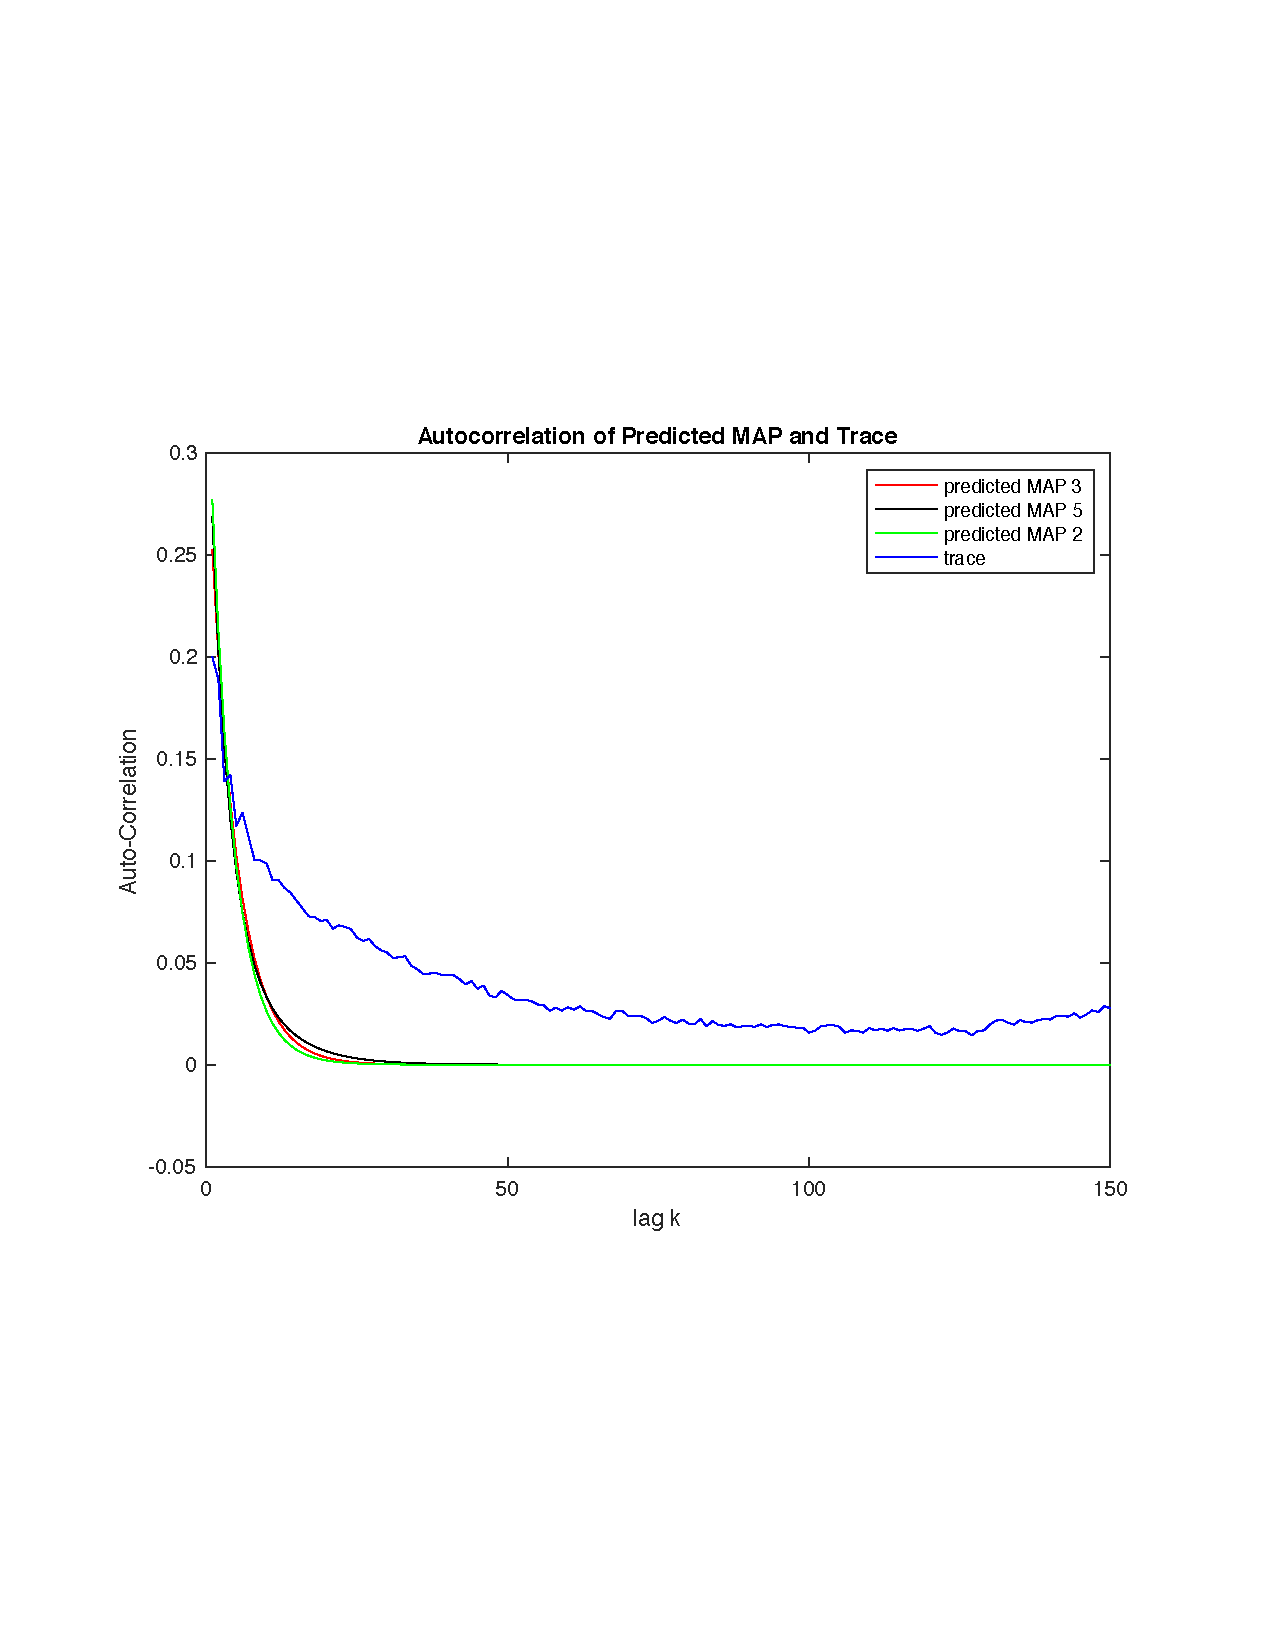
\includegraphics[width=100mm, scale=0.5]{bcgaug89_ac.pdf}
\caption{Auto-correlation of Predicted MAP of Order 3 and Trace Data}
\label{fig:bcaug_ac}
\end{center}
\end{figure}

We have that the best solution as determined by the log-likelihood is the MAP made with 8 orders. This makes sense, as we have that the trace is surely made from quite a complicated queueing system. Our best solution for this trace is the MAP made of the following matrices: 

\begin{equation}
    \mathbf{D}_0 = 10^3*\begin{bmatrix}
-0.087    &    0    &     0     &    0     &    0    &     0    &     0     &    0 \\
0 &  -4.34    &     0     &    0     &    0         0     &    0    &     0 \\
 0    &     0 &  -0.94  &  0.94  &      0    &     0    &     0    &     0 \\
  0     &    0     &    0   &  -0.94  &  0.94  &       0    &     0    &     0 \\
   0    &     0    &     0    &     0  &  -0.94   &      0     &    0    &     0 \\
 0    &     0    &     0   &      0     &    0  & -1.87  &  1.87   &      0 \\
  0     &    0    &     0     &    0     &    0   &      0  & -1.87  &  1.87 \\
0     &    0     &    0    &     0    &     0    &     0    &     0 &  -1.87
    \end{bmatrix}
\end{equation}

\begin{equation}
    \mathbf{D}_1 = 10^3*\begin{bmatrix}
0.0682  &  0.0002  &  0.0074    &   0   &  0   & 0.0106   &  0   &   0 \\
0.0132  &  0.2410  &  0.9681   &    0    &     0  &   3.1136     &    0    &     0 \\
0    &     0    &     0     &    0    &     0   &      0    &     0   &      0 \\
0    &     0     &    0     &    0    &     0   &      0    &     0     &    0 \\
0.0207  &  0.0546  &  0.8462    &     0   &      0 &   0.0158     &    0    &     0 \\
0    &     0     &    0     &    0    &     0   &      0    &     0     &    0 \\
0    &     0     &    0     &    0    &     0   &      0    &     0     &    0 \\
0.0595  &  0.3468  &  0.0412    &     0   &      0  &  1.4245    &     0    &     0 
    \end{bmatrix}
\end{equation} \\

Figure \ref{fig:bcaug_cdf} shows the cumulative distribution of the trace and the fitted MAPs. We have that the our prediction maps the cdf almost perfectly to that of the trace, which suggests that our algorithm fits to the trace well for this metric. 

\begin{figure}[h!]
\begin{center}
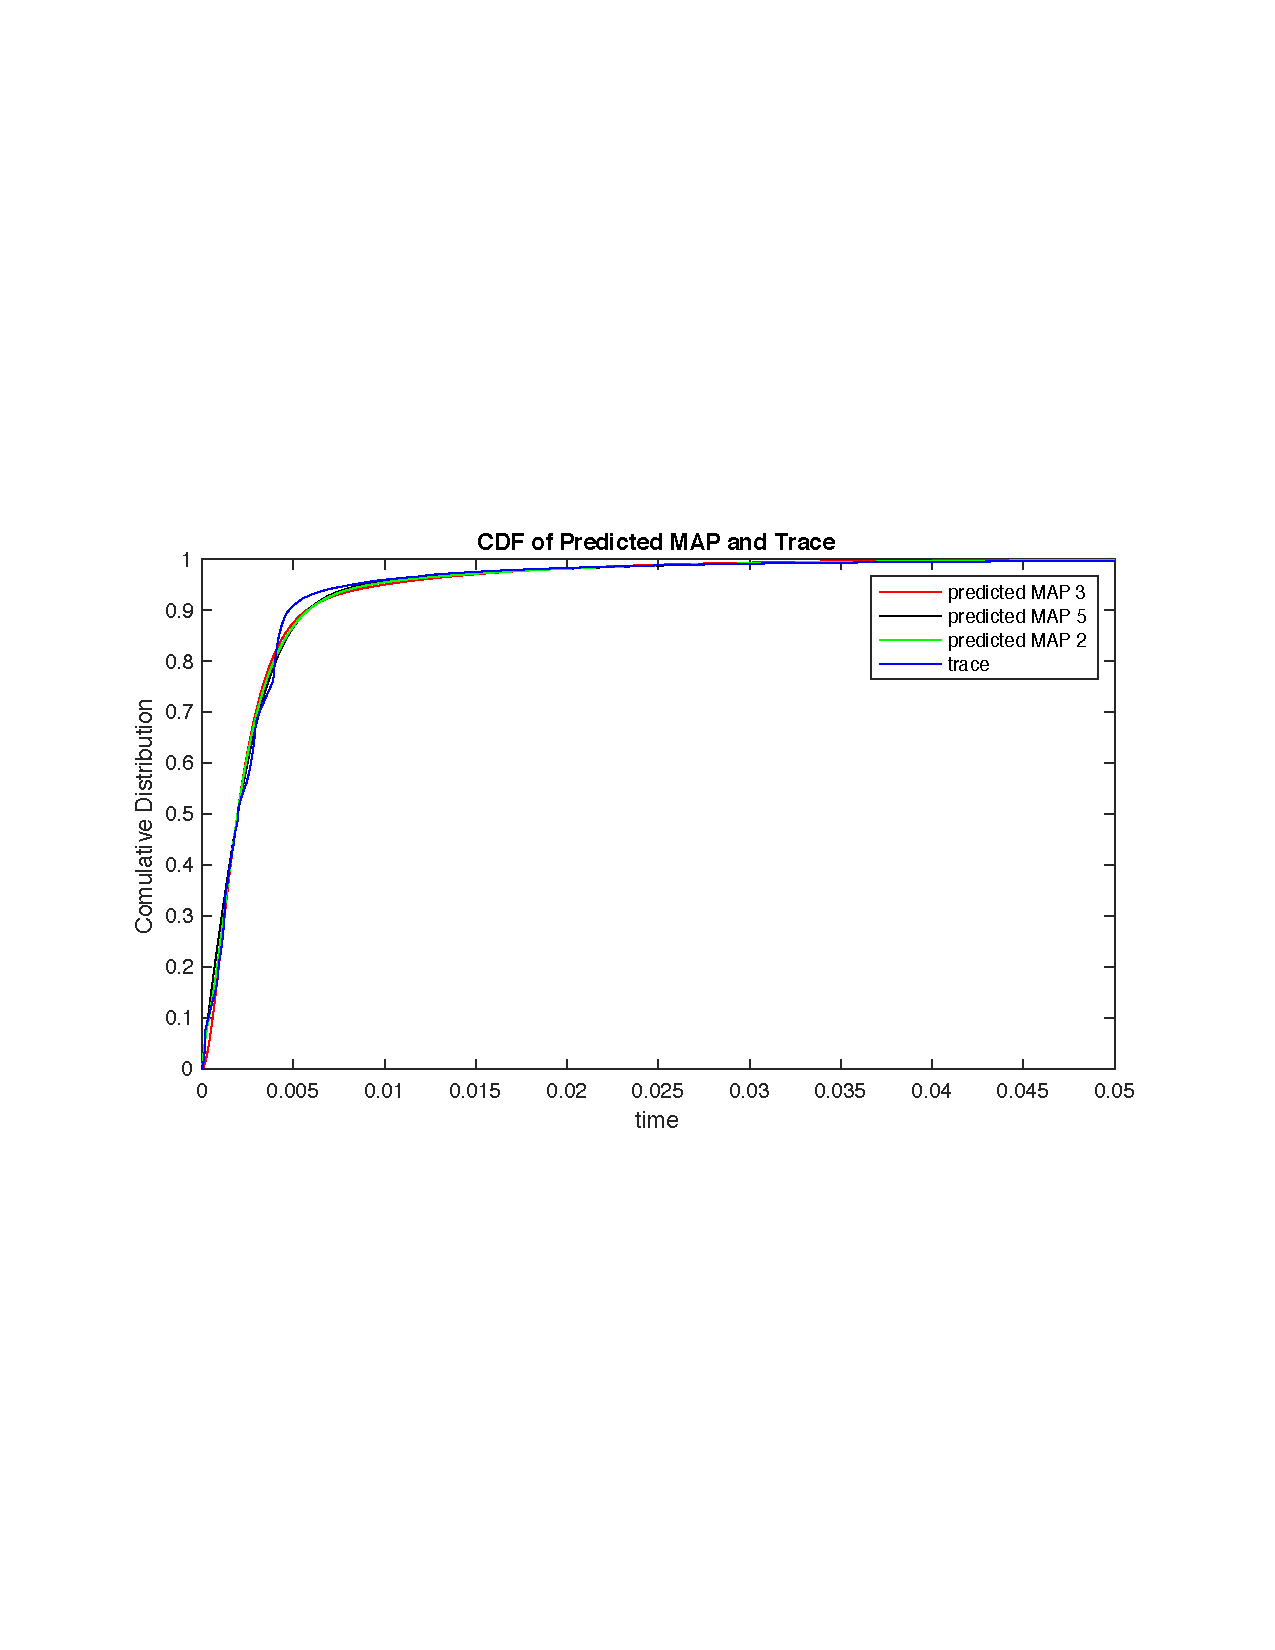
\includegraphics[width=100mm, scale=0.5]{bcaug_cdf.pdf}
\caption{Auto-correlation of Predicted MAP of Order 3 and Trace Data}
\label{fig:bcaug_cdf}
\end{center}
\end{figure}

\subsubsection{Example of a Real Trace Measured from Traffic between Digital Equipment Corporation and the Rest of the World}

We will now consider an example of a real world trace that contains an hour's worth of all wide-area traffic between Digital Equipment Corporation and the rest of the world [ITA]. We will try to fit an MAP to this trace in a similar way to the previous example. We will show the auto-correlation of the trace and the MAPs, as well as the associated distribution functions to evaluate how well we have predicted the parameters. Figure \ref{fig:pkt_ac} shows the auto-correlation of the fitted MAPs and that of the trace. We have that the best MAP is of order 3 and is shown to match the auto-correlation fairly well for the first 5 lag values. Afterwards, we have that we under-predict the auto-correlation until about the 90th lag point where the auto-correlations seem to match again. We have that the the auto-correlation for the trace keeps changing for 1000s of lags, and the fitted MAPs do not change after around the 100th lag, so we have not included this in the figure. Again, we can confirm that for larger values of lag we have not predicted the long-range dependencies well. Therefore, potentially the distribution function of the MAP and the trace will show us more in regards to the quality of our prediction. 

\begin{figure}[h!]
\begin{center}
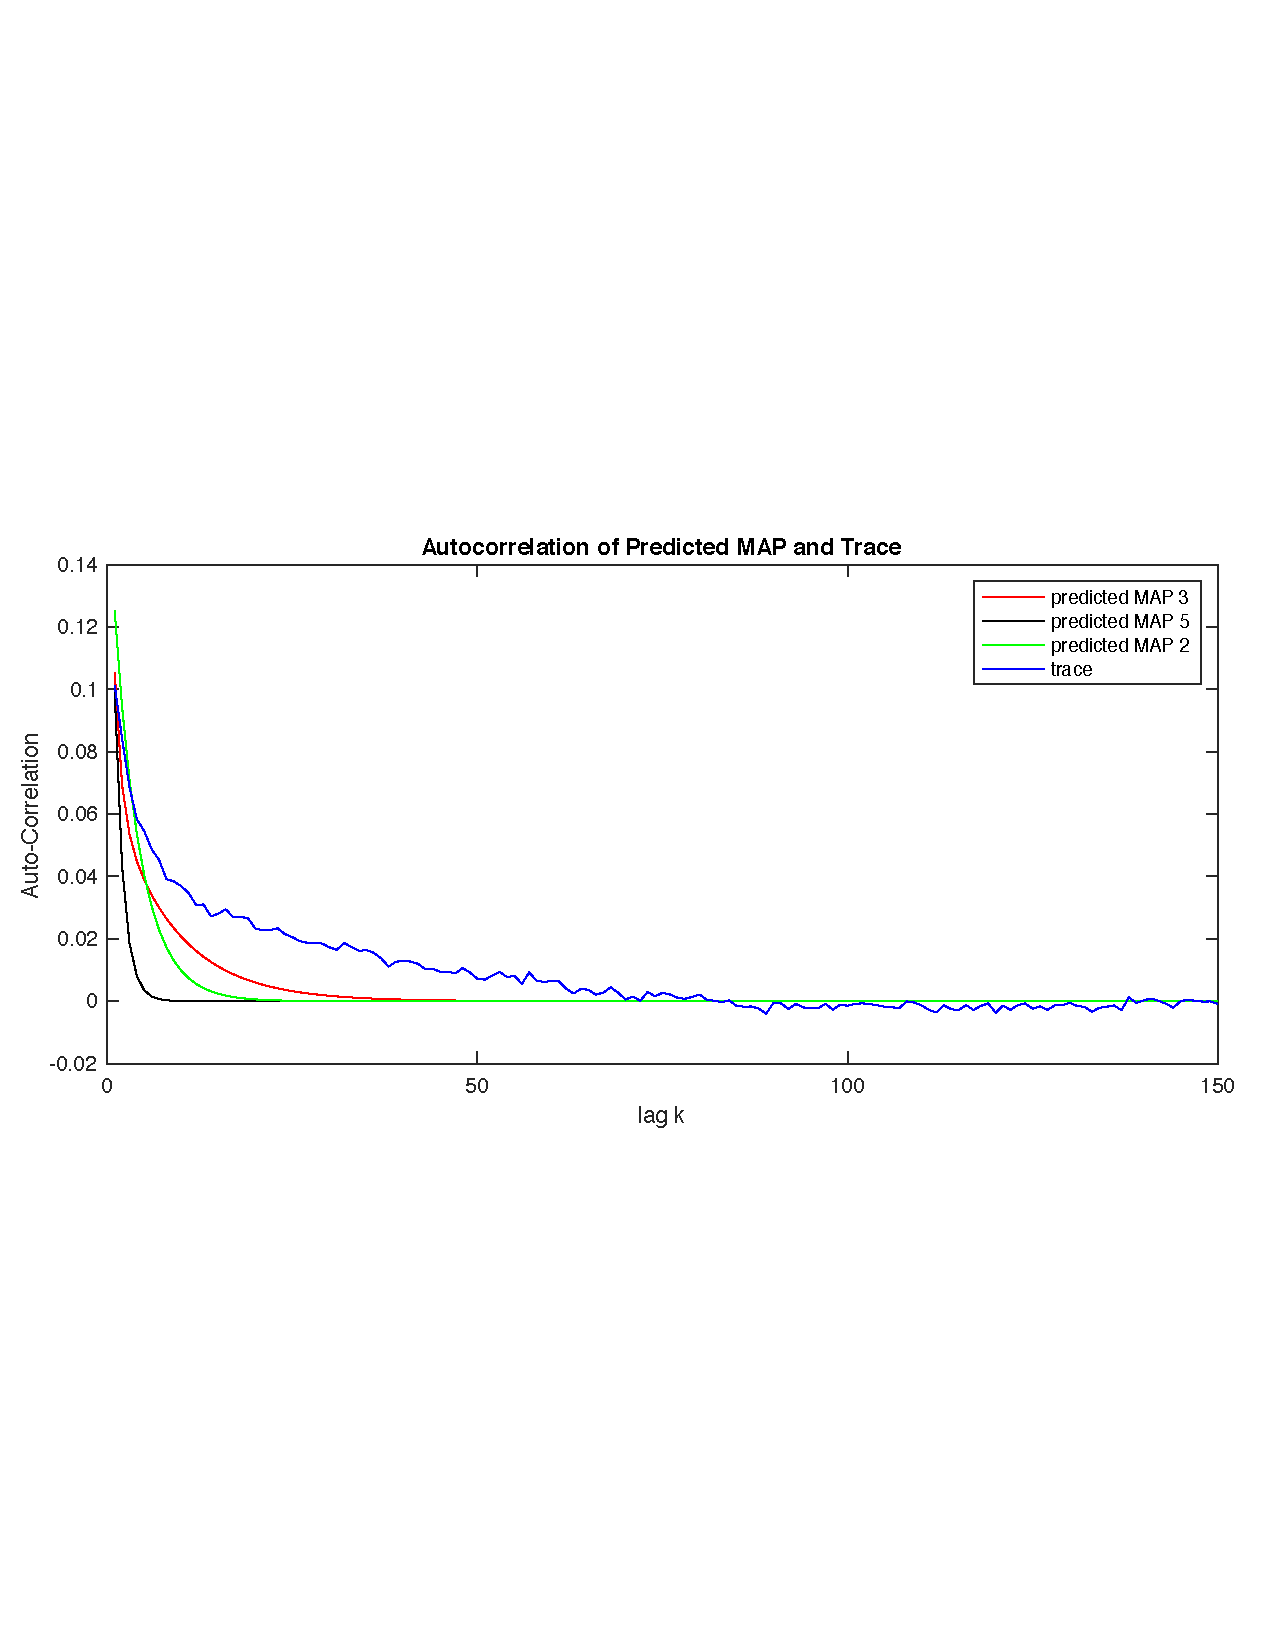
\includegraphics[width=100mm, scale=0.5]{pkt_ac.pdf}
\caption{Auto-correlation of Predicted MAPs and Trace Data for PKT trace}
\label{fig:pkt_ac}
\end{center}
\end{figure}

We have that the cumulative distribution function for each fitted MAP and the trace match each other extremely well, as is shown in Figure \ref{fig:pkt_cdf}. This suggests that we have predicted the correct parameters for our MAP from the real data trace.  

\begin{figure}[h!]
\begin{center}
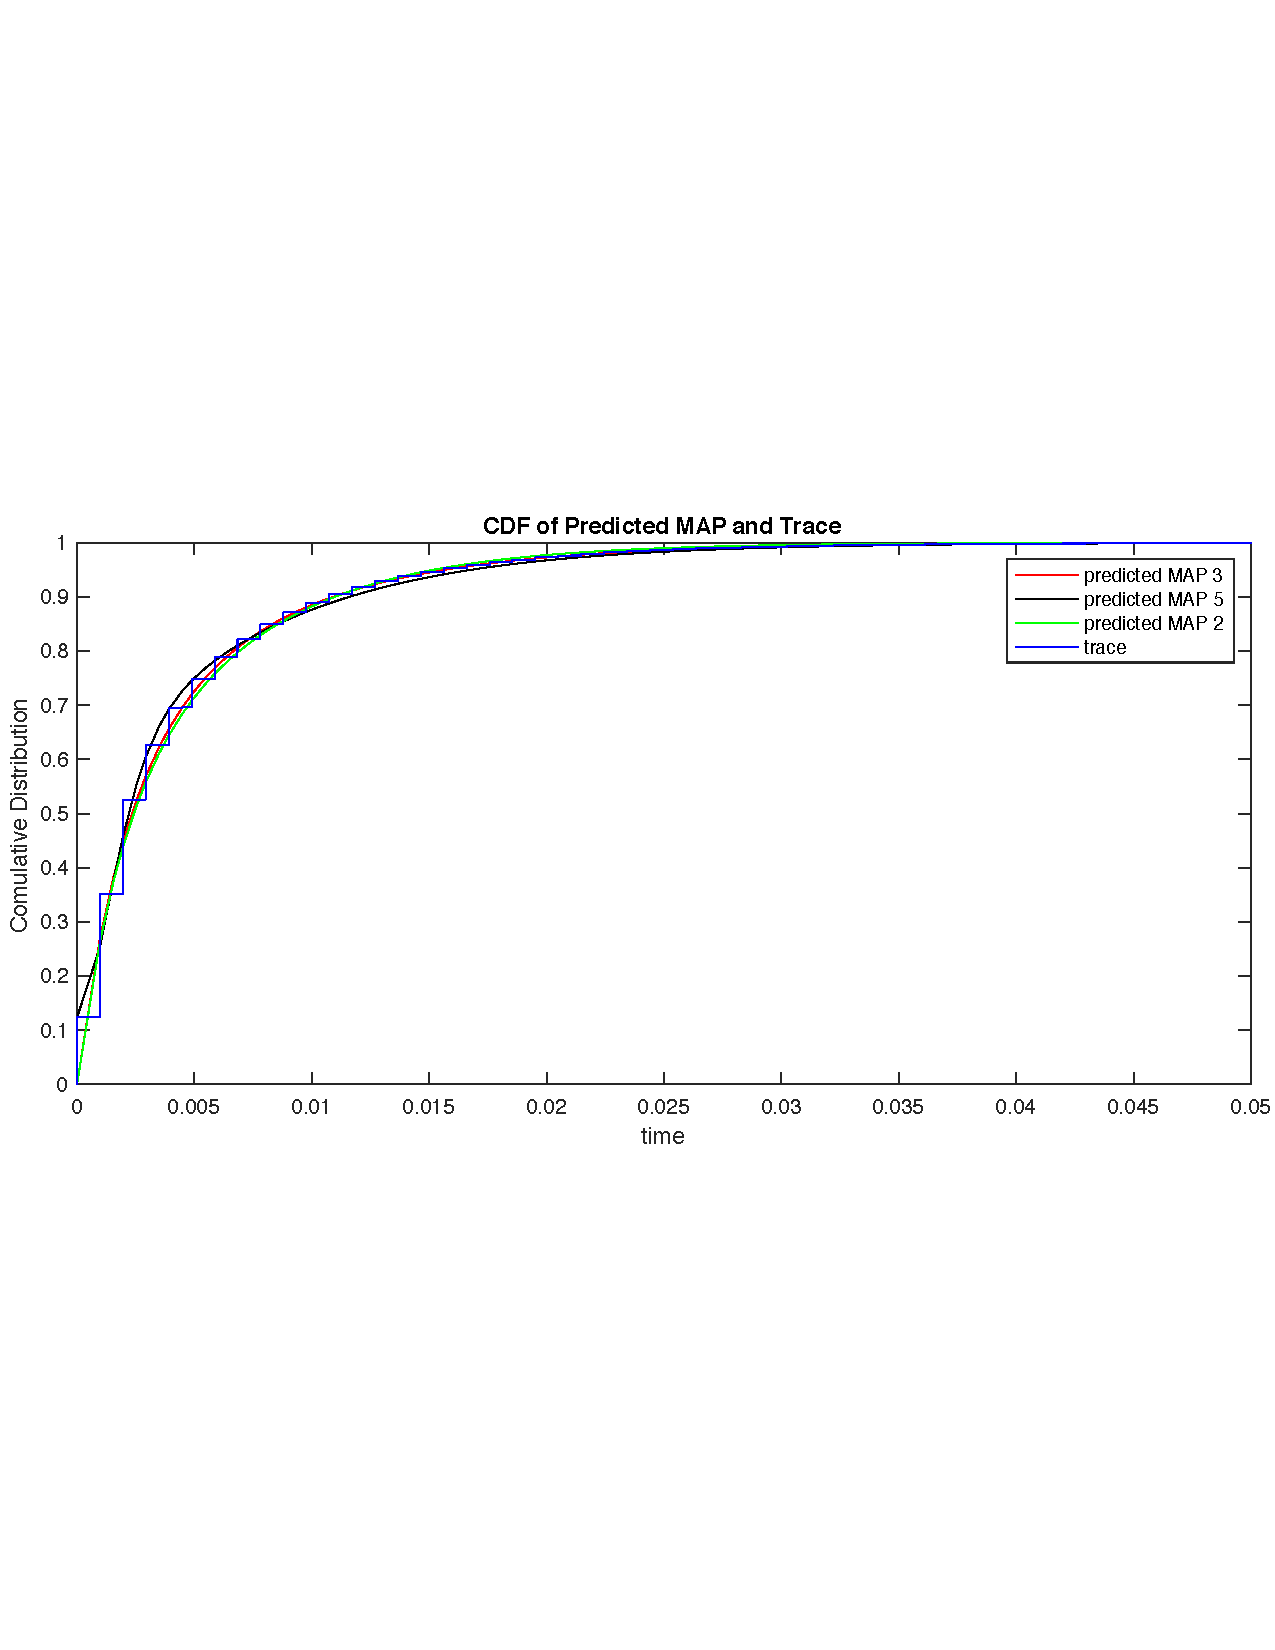
\includegraphics[width=100mm, scale=0.5]{pkt_cdf.pdf}
\caption{Cumulative Distribution Function of Predicted MAPs and Trace Data}
\label{fig:pkt_cdf}
\end{center}
\end{figure}


\subsection{Conclusions of our EM Algorithm}

We have applied our EM algorithm to many different examples. As was explained previously, the EM algorithm is not guaranteed to work. Given certain situations, we could find ourselves fall into a local optimum for our prediction, or just fail in our prediction altogether due to the high non-linearity of the parameters that we are trying to predict. Therefore, to evaluate our algorithm we had to choose many different examples and analyse the quality of our predictions. \\

Firstly, we analysed our algorithm when applied to trivial examples of MAPs built from simple queueing systems such as the M/M/1 queue and the M/G/1 queue. We found that for both of these our algorithm worked very well, and the corresponding predicted means, variances and auto-correlations were all very good matches to those of the real MAPs. \\

Secondly, we analysed our algorithm when applied to more complicated examples of MAPs built from machine repairman models. We chose three examples of differing complexity, where we increased the number of stations to increase the complexity. We found that for our first example, the predicted MAP matched the auto-correlation of the real MAP extremely well and we had no issues. For the second and third examples, we found it much harder to match the auto-correlation. We decided to analyse the quality of our predicted MAP by considering the distribution functions of the MAPs and the trace. The distribution functions gave almost perfect results. When we couple this result with the results for the mean and the variance of the MAPs, we found that our algorithm predicted the parameters of the MAP extremely well. \\

Lastly, we looked at real data situations, where we took traces from LAN traffic and Digital Equipment traffic. We found a similar trend in both: the auto-correlation of the trace was difficult to predict accurately, however the distribution had a very accurate prediction. This is most likely because our EM algorithm works by using likelihoods and optimizing matrix values, instead of optimizing the moments of the trace. As we had great predictions for the distribution, we can conclude that our EM algorithm works very well at predicting parameters of MAPs, and can easily be used for real world data as well. There have been other approaches to fitting real trace date with the EM algorithm, as can be seen in [Rac03], which fits world-wide web request traces, and [Buc03] which fits real traffic system traces.

\section{Markov Chain Monte Carlo Methods for Parameter Fitting}

\subsection{Setting of the Problem and Initial Description of Parameters}

This section will focus on a Bayesian approach to parameter inference in queueing networks, specifically by using Markov-Chain Monte Carlo methods to infer parameters. We will define inference based on queue-length data by observing equilibrium state distributions of queueing network models. From references such as [Bol06], it is well known that the equilibrium distribution of queue lengths is relatively easy to deal with. To explain this, we will briefly discuss the BCMP theory regarding queueing networks. A BCMP network is a class of queueing network where a product-form equilibrium distribution exists. Therefore, under BCMP theorem assumptions, we have that the equilibrium of queue lengths takes a convenient product-form expression [Igl19]. Therefore, from this assumption, the BCMP equilibrium distribution is suitable to define Bayesian inference estimations. We define a BCMP network as a queuing network with $M$ queueing nodes and $R$ job classes [Bal01]. We have that the nodes can be one of four types: First Come First Served, where the service time distributions are the same for all classes; Processor Sharing, where each waiting job gets an equal share of the capacity and the service distributions are of a Coxian type; Infinite Server, where an infinite number of servers are available; or Last Come First Served with Preemption. We also assume that in our model we have $K_j$ jobs for each class $j$, and they have a known average `think' time denoted by $Z_j > 0$. After a job is serviced, the `think' time is the interval at which a job waits at the user-terminal before it cycles again. We assume that the system is at steady-state and samples of its
state are sufficiently spaced in time to be approximately independent
of each other [Bal01]. We denote the number of jobs of class $j$ in station $i$ as $n_{ij}$, and $\theta_{ij}$ as the demand of class $j$ requests at station $i$. $\theta_{ij}$ is the product of the mean service time of a request and the mean number of visits of the request at resource $i$ before completion [Bal01]. We denote the service demand matrix as $\bm{\theta} = \{\theta_{ij}\}$, where $1 < i \leq M$ and $1 < j \leq R$. Using our assumptions on the queueing network, we have that the probability of state $\mathbf{n} = \{n_{ij}\}$ gives the following product-form expression [Cas16]: 

\begin{equation}
    P(\mathbf{n}|\bm{\theta}) = \frac{Z_1^{n_{01}}}{n_{01}!}...\frac{Z_R^{n_{0R}}}{n_{0R}!} \prod_{i=1}^{M} n_{i}! \prod_{j=1}^{R} \frac{\theta_{ij}^{n_{ij}}}{n_{ij}!G(\bm{\theta})}
    \label{eqn:state_probs}
\end{equation}

where $G(\bm{\theta})$ denotes the normalizing constant of the state probabilities under the restriction that $\sum_{\mathbf{n}} P(\mathbf{n}|\bm{\theta}) = 1 $. We express $G(\bm{\theta})$ in terms of the service demands, instead of the more common dependence on job populations. The underlying aim of this section is to estimate the parameters $\theta_{ij}$ given observations of the state probabilities, as well as the vector of mean think times $\mathbf{Z}$. If we were to not know the mean waiting times, then two closed networks that have different parameters $\theta_{ij}$ could be indistinguishable from one another and have identical distribution of stationary stationary queue length [Cas13]. \\

Within our Bayesian setting, we see the observations of the state probabilities shown in Equation \ref{eqn:state_probs} as the likelihood of the observing state $\mathbf{n}$ given a particular estimate of the unknown parameters $\theta_{ij}$. There is a complication in finding these values due to the presence of the normalization constant $G(\bm{\theta})$, which involves expensive computations [Cas16]. Therefore, we must examine a technique to first evaluate the normalization constant $G(\bm{\theta})$ to help us evaluate the likelihood functions, before using an MCMC search algorithm to estimate the service demand parameters $\theta_{ij}$. In this section, as detailed by the references [Cas16] and [Cas13], we will define a Taylor expansion algorithm to help us determine the normalization constant, and then we will use the MCMC method Gibbs Sampling in order to accurately estimate the parameters. 

\subsection{Taylor Expansion Method for Analysing the Normalization Constant}

In this section we offer an algorithm to determine the computationally expensive normalization constant using the Taylor expansion (TE) method. The aim of this section is to analyse a method for finding the normalization constant $G(\bm{\theta})$ such that we can compute the likelihood function detailed in Equation \ref{eqn:state_probs}. The approach detailed here follows that described in [Cas16], where we apply a Taylor Expansion of $G(\bm{\theta})$ along a dimension of the demands $\bm{\theta}$, and use an approximate mean value analysis (AMVA) algorithm iteratively to estimate the first-order derivative in the expansion. Within our description of the TE algorithm there are many calculations that we will not prove in this paper. To get a better understanding of the mathematical proof of certain equations we will provide the references that explain them in more detail. Most of the following equations have been adapted from [Cas16]. \\

From a sensitivity analysis of queueing networks, Equation \ref{eqn:sens_analysis} arises:

\begin{equation}
    \frac{d G(\bm{\theta})}{d \bm{\theta_{ij}}} = \frac{Q_{ij}(\bm{\theta})}{\theta_{ij}} G(\bm{\theta})
    \label{eqn:sens_analysis}
\end{equation}

where $Q_{ij}$ represents the average queue length of jobs at station $i$ of class $j$. We now define a Taylor expansion of $G(\bm{\theta})$ in Equation \ref{eqn:TE_nc}:

\begin{equation}
    G(\bm{\theta} + d \bm{\theta_{ij}}) = G(\bm{\theta}) + \frac{d G(\bm{\theta})}{d \bm{\theta}_{ij}} d\bm{\theta}_{ij} + o(\theta_{ij}^2)
    \label{eqn:TE_nc}
\end{equation}

where $d \bm{\theta}_{ij}$ updates updates the dimension $ij$ exclusively. We then substitute Equation \ref{eqn:sens_analysis} into Equation \ref{eqn:TE_nc} for the differential to obtain: 

\begin{equation}
    G(\bm{\theta} + \Delta \bm{\theta}_{ij}) \approx G(\bm{\theta}) \left(1+\frac{Q_{ij}(\bm{\theta})}{\theta_{ij}}\right) \Delta \theta.
    \label{eqn:TE_G}
\end{equation}

The term $\Delta \bm{\theta}_{ij} = \Delta \theta_{ij} \mathbbm{1}_{ij}$ where $\mathbbm{1}_{ij}$ denotes a zero vector except for a 1 in position $ij$. The term $\Delta \theta$ represents the `step size'. We then take the logarithm of Equation \ref{eqn:TE_G} to work with sums instead of products such that we can more easily evaluate the expression iteratively. Taking the logarithm gives the following equation:

\begin{equation}
    log(G(\bm{\theta} + \Delta \bm{\theta}_{ij})) \approx log G(\bm{\theta}) + log \left(1+\frac{Q_{ij}(\bm{\theta})}{\theta_{ij}}\right) + log \Delta \theta
    \label{eqn:log_TE_G}
\end{equation}

where we can iteratively evaluate Equation \ref{eqn:log_TE_G} at each step for increasing values of $\theta_{ij}$ [Cas13]. We iteratively evaluate $G(\bm{\theta})$ using TE as follows [Cas16]: 

\begin{enumerate}
    \item Start from an arbitrary value of $\bm{\theta}$ for which $G\bm({\theta})$ is known, such as setting all $\theta_{ij}$ to zero such that $G(\mathbf{0}) = \prod_{j=1}^{R} Z_{j}^{N_j}/N_j!$. 
    \item Iterate Equation \ref{eqn:TE_G} along all dimensions of $\bm{\theta}$ successively.
    \item Initialize the first invocation of the AMVA with a balanced distribution of jobs across the stations.
    \item For each dimension, add $\Delta \theta$ to $\theta_{ij}$ and compute $G(\bm{\theta} + \Delta \bm{\theta}_{ij})$ from the previous value of $G({\bm{\theta}})$ using Equation
    \ref{eqn:log_TE_G}. The $Q_{i,j}(\bm{\theta})$ values are found using an AMVA algorithm, with an initializing of the mean queue lengths computed at the `last invocation of AMVA' [Cas16].
    \item We obtain the value of $log(G(\bm{\theta}))$ and use the exponential function to find $G(\bm{\theta})$. 
\end{enumerate}

There are other ways to evaluate the normalization constant, such as ICMI and MCI methods. It is fascinating to observe which technique gives the fastest and more accurate results, however we will not delve into this topic in this paper. Within our numerical evaluation, we will use a method to obtain the normalizing constant that has already been implemented in LINE [Lin20]. This is mainly due to time constraints of the project, but also because this method is very efficient and will give us favourable results. 

\subsection{Gibbs Sampling Algorithm for Demand Estimation}

In this section we will explore the suitability of using the MCMC method Gibbs Sampling for demand estimation of queueing networks, where we observe a sequence $\mathbf{N} = \{\mathbf{n}^{(1)}, ..., \mathbf{n}^{(D))}\}$ of independent states. Each $\mathbf{n}^{(i)}$ denotes the $i$th observed state, where $1 \leq i \leq D$ [Cas16]. We will now define the notation that we will use when referencing Gibbs sampling [Cas16]: 

\begin{enumerate}
    \item $S$: the number of samples that we will generate. 
    \item $D$: the number of observations that are provided.
    \item $\mathbf{N}$: the input data set. 
    \item $\Delta \theta$: the step size. 
    \item $\mathbf{I}$: the discretization range.
\end{enumerate}

Given that $S$ denotes the number of samples that we draw from the Gibbs sampling, we define $\theta_{ij}^{s}$ as the $s$th sample that is generated from estimating the demand $\theta_{ij}$. A sample $\theta_{ij}^{s}$ follows the distribution given by $P(\theta_{ij}|\bm{\theta}_{ij}^{s}, \mathbf{N})$, where $\bm{\theta}_{(ij)}^{s} = (\theta_{11}^{s}, ..., \theta_{i,(j-1)}^{s},\theta_{i,(j+1)}^{s-1},...,\theta_{MR}^{s-1})$ is evaluated using past generated samples. The samples that we generate will have a distribution that converges to the posterior density function for demands $\theta_{ij}$, given the priors and the observed data. We use the TE method to efficiently compute the difficult computation of the conditional distributions $P(\theta_{ij}|\bm{\theta}_{ij}^s, \mathbf{N})$. For each demand $\theta_{ij}$, we use the following conditioning [Cas16]: 

\begin{equation}
    P(\theta_{ij}|\bm{\theta}_{ij}^s, \mathbf{N}) = 
   \frac{ P(\theta_{ij},\bm{\theta}_{ij}^{s}|\mathbf{N})}{\int P(\hat{\theta}_{ij}, \bm{\theta}_{ij}^s|\mathbf{N})d \hat{\theta}_{ij}}.
   \label{eqn:condit_dist}
\end{equation}

We use Bayes' theorem on Equation \ref{eqn:condit_dist} to obtain: 

\begin{equation}
    P(\theta_{ij}|\bm{\theta}_{ij}^s, \mathbf{N}) = 
     \frac{ P(\theta_{ij},\bm{\theta}_{ij}^{s}) P(\mathbf{N}| \theta_{ij}, \bm{\theta}_{(ij)}^{s})}{\int P(\hat{\theta}_{ij},\bm{\theta}_{ij}^{s}) P(\mathbf{N}| \hat{\theta}_{ij}, \bm{\theta}_{(ij)}^{s})d \hat{\theta}_{ij}}
     \label{eqn:condit_dist_bayes}
\end{equation}

where we note that the integral present in the denominator can be evaluated as a constant independent of $\theta_{ij}$. Therefore, we achieve a directly proportional formula for the conditional distribution as shown in Equation \ref{eqn:prop_dist}:

\begin{equation}
    P(\theta_{ij}|\bm{\theta}_{ij}^s, \mathbf{N}) \propto P(\theta_{ij},\bm{\theta}_{ij}^{s}) P(\mathbf{N}| \theta_{ij}, \bm{\theta}_{(ij)}^{s})
    \label{eqn:prop_dist}
\end{equation}

which, once we consider the assumed independence of observations, becomes:

\begin{equation}
    P(\theta_{ij}|\bm{\theta}_{ij}^s, \mathbf{N}) \propto \prod_{\mathbf{n} \in \mathbf{N}} P(\theta_{ij},\bm{\theta}_{ij}^{s}) P(\mathbf{n}| \theta_{ij}, \bm{\theta}_{(ij)}^{s}).
\end{equation}

and the term $P(\mathbf{n}| \theta_{ij}, \bm{\theta}_{(ij)}^{s})$ denotes the likelihood of observing state $\mathbf{n}$ for a given $\theta_{ij}$ and the past samples of demands [Won09]. We have already shown that the likelihood function can be computed fairly easily using the equilibrium distribution of the network shown in Equation \ref{eqn:state_probs}. Finally, we draw a sample from the distribution $P(\theta_{ij}|\bm{\theta}_{ij}^{s},\mathbf{N})$. We take $\theta_{ij}$ as a finite quantity, therefore we assume that it lies in the discretization range $\mathbf{I} = [\theta_{ij}^{-},\theta_{ij}^{+}]$. 
We condition on $\theta_{ij} \in \mathbf{I}$, and subsequently define the cumulative distribution of demands in this interval as follows: 

\begin{equation}
    F(\theta_{ij}|\bm{\theta}_{ij}^{s}, \mathbf{N}) = \int_{\theta_{ij}^{-}}^{\theta_{ij}} P(\hat{\theta}_{ij}|\bm{\theta_}{ij}^{s}, \mathbf{N}) d \hat{\theta}_{ij}.
    \label{eqn:cum_dist_mcmc}
\end{equation}

We then utilize Equation \ref{eqn:prop_dist} and initialize using Equation \ref{eqn:state_probs} to represent Equation \ref{eqn:cum_dist_mcmc} as: 

\begin{equation}
     F(\theta_{ij}|\bm{\theta}_{ij}^{s}, \mathbf{N}) = \frac{1}{H(\bm{\theta}_{ij}^{s})} \int_{\theta_{ij}^{-}}^{\theta_{ij}} \prod_{\mathbf{n} \in \mathbf{N}} \left( G^{-1} (\hat{\theta}_{ij}, \bm{\theta}_{ij}^{s}) \hat{\theta}_{ij}^{n_{ij}} \right) P(\hat{\theta}_{ij}, \bm{\theta}_{ij}^{s}) d \hat{\theta}_{ij}
     \label{eqn:cum_dist_prod}
\end{equation}

where we define $H(\bm{\theta}_{ij}^{s})$ as: 

\begin{equation}
    H(\bm{\theta}_{ij}^{s}) = \int_{\theta_{ij}^{-}}^{\theta_{ij}^{+}} \prod_{\mathbf{n} \in \mathbf{N}} \left( G^{-1} (\hat{\theta}_{ij}, \bm{\theta}_{ij}^{s}) \hat{\theta}_{ij}^{n_{ij}} \right) P(\hat{\theta}_{ij}, \bm{\theta}_{ij}^{s}) d \hat{\theta}_{ij}
    \label{eqn:H_nc}
\end{equation}

which acts as a normalizing constant to ensure that $F(\theta_{ij}^{+}) = 1$. We note that in Equations \ref{eqn:cum_dist_prod} and \ref{eqn:H_nc} we have not included the contributions of the factorials in Equation \ref{eqn:state_probs}. We can simplify these terms by grouping them in in front of the integrals in those equations. Hence, we can break apart the product notation in these expressions for $\mathbf{N}$ to observe that the cumulative distribution function can be re-written as: 

\begin{equation}
    F(\theta_{ij}|\bm{\theta}_{ij}^{s}, \mathbf{N}) = \frac{1}{H(\bm{\theta}_{ij}^{s})} \int_{\theta_{ij}^{-}}^{\theta_{ij}}\left( G^{-1} (\hat{\theta}_{ij}, \bm{\theta}_{ij}^{s}) \right)^D \prod_{\mathbf{n} \in \mathbf{N}} \hat{\theta}_{ij}^{n_{ij}} P(\hat{\theta}_{ij}, \bm{\theta}_{ij}^{s}) d \hat{\theta}_{ij} \\
    \label{eqn:final_dist_gibbs}
\end{equation}

$$ = \frac{1}{H(\bm{\theta}_{ij}^{s})} \int_{\theta_{ij}^{-}}^{\theta_{ij}}\left( G^{-1} (\hat{\theta}_{ij}, \bm{\theta}_{ij}^{s},\hat{\theta}_{ij}^{\hat{n}_{ij}}) \right)^D P(\hat{\theta}_{ij}, \bm{\theta}_{ij}^{s}) d \hat{\theta}_{ij}$$

where now we have an expression for the cumulative distribution that only depends upon the average queue lengths $\hat{n}_{ij} = \sum_{\mathbf{n} \in \mathbf{N}} n_{ij}/D$ of the system, and the number of observations $D$. This is a very important observation, as it means that the only data that we need to consider when performing Gibbs sampling is the mean queue lengths $\hat{n}_{ij}$, instead of information from detailed system states $\mathbf{n}$ [Cas16], [Cas13] and [Won09]. The above equations are used within the Gibbs sampling algorithm, which we will now detail exactly in steps below which have been adapted from [Cas16], [Cas13]:  \\

\textbf{Gibbs Sampling Procedure:}

\begin{enumerate}
    \item Input: $\mathbf{N}$, $\mathbf{I}$, $M$, $R$, $\mathbf{K}$, $S$, $\mathbf{Z}$, $\Delta \theta_{ij}$.
    \item $\bm{\theta}^0 = (\theta_{11}^{-}, ... , \theta_{MR}^{-})$. 
    \item Evaluate $logG(\bm{\theta}^0)$.
    \item For $s = 1:S$ do:
    \begin{enumerate}
        \item For $i=1:M$ do:
        \begin{enumerate}
            \item For $j=1:R$ do:
            \begin{enumerate}
            \item Set $\bm{\theta}_{ij}^{s} = (\theta_{11}^{s},...,\theta_{i,j-1}^{s},\theta_{i,j+1}^{s-1}, ..., \theta_{MR}^{s-1})$. 
            \item Evaluate $log G(\hat{\theta}_{ij}, \bm{\theta}_{ij}^{s}) \: \forall \: \hat{\theta}_{ij} \in [\theta_{ij}^{-}, \theta_{ij}^{+}]$ using step-size $\Delta \theta_{ij}$. 
            \item Psuedo-randomely generate a number $u \in [0,1]$. 
            \item Find $\theta_{ij}^{s}$: $F(\theta_{ij}^{s} | \bm{\theta}_{ij}^{s}, \mathbf{N}) \leq u < F(\theta_{ij}^{s} + \Delta \theta_{ij}|\bm{\theta}_{ij}^{s}, \mathbf{N})$.
            \end{enumerate}
        \end{enumerate}
    \end{enumerate}
    \item Return $\theta_{ij}^{s} \: \forall \: s, i, j$. 
\end{enumerate}

In our implementation we set the initial vector $\bm{\theta}_{ij}^{(s)}$ full of zeros. We also define a prior distribution as an input to the function. The set of samples that we return can be used either directly to determine the demand estimates, or numerically to estimate the posterior density of the demands. When we generate samples, we only use half of them in the algorithm. This is to take into consideration the `burn in' time caused by the transient in the underlying Markov chain [Cas16]. Therefore, if we generate $S=60$ samples for each demand, we only use the last 30 samples to estimate the service demands. For the application of Gibbs sampling we need to define the prior distribution $P(\bm{\theta})$. Priors are very important, especially when the size of the dataset is small. There are substantial interesting priors that we could use and investigate. In our algorithm we will focus on using a uniform distribution for the prior, where each parameter $\theta_{ij}$ is equally likely in the range $[\theta_{ij}^{-}, \theta_{ij}^{+}]$ [Won09]. Our methodology can accept any arbitrary prior however, such as a Jeffrey prior or a Dirichlet prior. Additionally, it is important to note that when we use our algorithm we will approximate the integrals in Equation \ref{eqn:final_dist_gibbs} using a TE method. We compute the integrals by `computing the integrand at a number of equidistant points, chosen with step $\Delta \theta_{ij}$, in the range $\mathbf{I}$.' [Cas16].

\subsection{Metropolis Hastings Algorithm for Demand Estimation}

In this section we will briefly discuss another MCMC method called Metropolis Hastings (MH) [Cas16] for the task of demand estimation. The MH algorithm takes a Markov chain with continuous state-space such that we sample from a target distribution $f(\bm{\theta})$. We are trying to estimate the demand estimation, therefore we set the target distribution as: $P(\bm{\theta}|\mathbf{N})$, which we use Bayes' theorem on to give the following expression [Cas13]:

\begin{equation}
    P(\bm{\theta}|\mathbf{N}) = \frac{P(\mathbf{N}|\bm{\theta}) P(\bm{\theta})}{P(\mathbf{N})} = \frac{\prod_{\mathbf{n} \in \mathbf{N}} P(\mathbf{n} | \bm{\theta}) P(\bm{\theta})}{P(\mathbf{N})}
    \label{eqn:bayes_MH}
\end{equation}

where we describe $P(\mathbf{N})$ as a normalizing constant that ensures $\sum_{\bm{\theta}} P(\bm{\theta}|\mathbf{N}) = 1$ [Cas16]. The algorithm is shown below in the following steps [Cas16]: 

\begin{enumerate}
    \item Generate a new parameter $\bm{\theta}$ from  a proposed distribution $q(\bm{\theta}|\bm{\theta}^{(t)})$ at time step $t+1$, where $\bm{\theta}^{(t)}$ is the demand vector sampled at the previous iteration.
    \item Compute an `acceptance rate' which determines whether we accept a generated sample: $$\alpha = \text{min} \left(1, \frac{P(\bm{\theta}|\mathbf{N}) q(\bm{\theta}^{(t)}|\bm{\theta})}{P(\bm{\theta}^{(t)}|\mathbf{N}) q(\bm{\theta}|\bm{\theta}^{(t)})} \right)$$
    \item Choose whether we accept the candidate with probability $\alpha$. If accepted, set $\bm{\theta}^{(t+1)} = \bm{\theta}$. If not accepted, set $\bm{\theta}^{(t+1)} = \bm{\theta}^{(t)}$. 
    \item After $S$ iterations, return the vector of accepted samples which are distributed according to the target distribution $f(\bm{\theta})$. 
\end{enumerate}
    
As explained in the paper [Cas16], we can implement demand estimation using MH by setting the proposed distribution for the sampling to a multivariate Gaussian distribution. The covariance matrix of this distribution is chosen to be $\beta \mathbf{I}$, where $\mathbf{I}$ is the identity matrix, and $\beta = 10^{-3}$ to `match the magnitude of the demands' [Cas16].


\section{Experimental Validation of the Gibbs Sampling Algorithm for Demand Estimation}

To evaluate our MCMC methods for demand estimation we need to apply our Gibbs sampling algorithm to many different example queueing systems. As detailed previously, the models that we use for demand estimation follow the BCMP format. Therefore, to analyse and evaluate our algorithm we will consider synthetically generated examples of many queueing networks that lie within this format. To use our algorithm for demand estimation we define the following parameters for the queueing network: the think times $Z_i$; the service demands that our algorithm aims to estimate $d_k$; the size of queueing stations $M$ and job classes $R$ in the system; the number of jobs in the network $K$; and the number of experiments $S$ that we perform in the algorithm. We then perform a hyper-parameter search on both the step size $\delta \theta$ and the total number of samples $D$ that we use in the algorithm. When we are changing the step-size, we keep the number of samples at $D = 10000$. When we change the number of samples, we set the step-size to $0.0001$. We use the following values for each parameter in our evaluation of the algorithm, regardless of what type of BCMP network we choose as an example queueing network: 

\begin{enumerate}
    \item S = 20.
    \item $\delta \theta = [0.001,0.0005]$.
    \item $K = [20,40,60,80]$.
    \item $D = [5000, 20000, 60000]$.
    \item $\mathbf{I} = [0,0.2]$.
\end{enumerate}

To evaluate our Gibbs sampling model we will use the mean absolute percentage error metric. This measures the average difference between our estimated demands $\hat{\bm{\theta}}$ and the real demands $\bm{\theta}$ using Equation \ref{eqn:mape}:

\begin{equation}
    err = \frac{1}{MR} \sum_{i=1}^{M} \sum_{j=1}^{R} \frac{|\hat{\theta}_{ij} - \theta_{ij}|}{\theta_{ij}}
    \label{eqn:mape}
\end{equation}

\subsection{Processor Sharing Queueing Network Serial Examples}

In this section we will evaluate how well our Gibbs sampling algorithm estimates the demands of Processor Sharing queueing networks. We will take different values of $M$ and $R$ and examine the error metric of our algorithm. 

\subsubsection{Example 1: 1 Station, 1 Class}

We start our evaluation examining the error of our Gibbs sampling algorithm on a trivial and simple queueing network consisting of 1 queueing node and 1 job class. We set the demand of the station to $1/20$, which is the metric that we are trying to estimate from using Gibbs sampling. Figure \ref{fig:M1R1_eval_gibbs} shows the error in estimating the demands when we alter both the step-size and the number of samples that we choose for our algorithm. We show the error against the number of jobs that populate the system. \\

\begin{figure}[h!]
\begin{center}
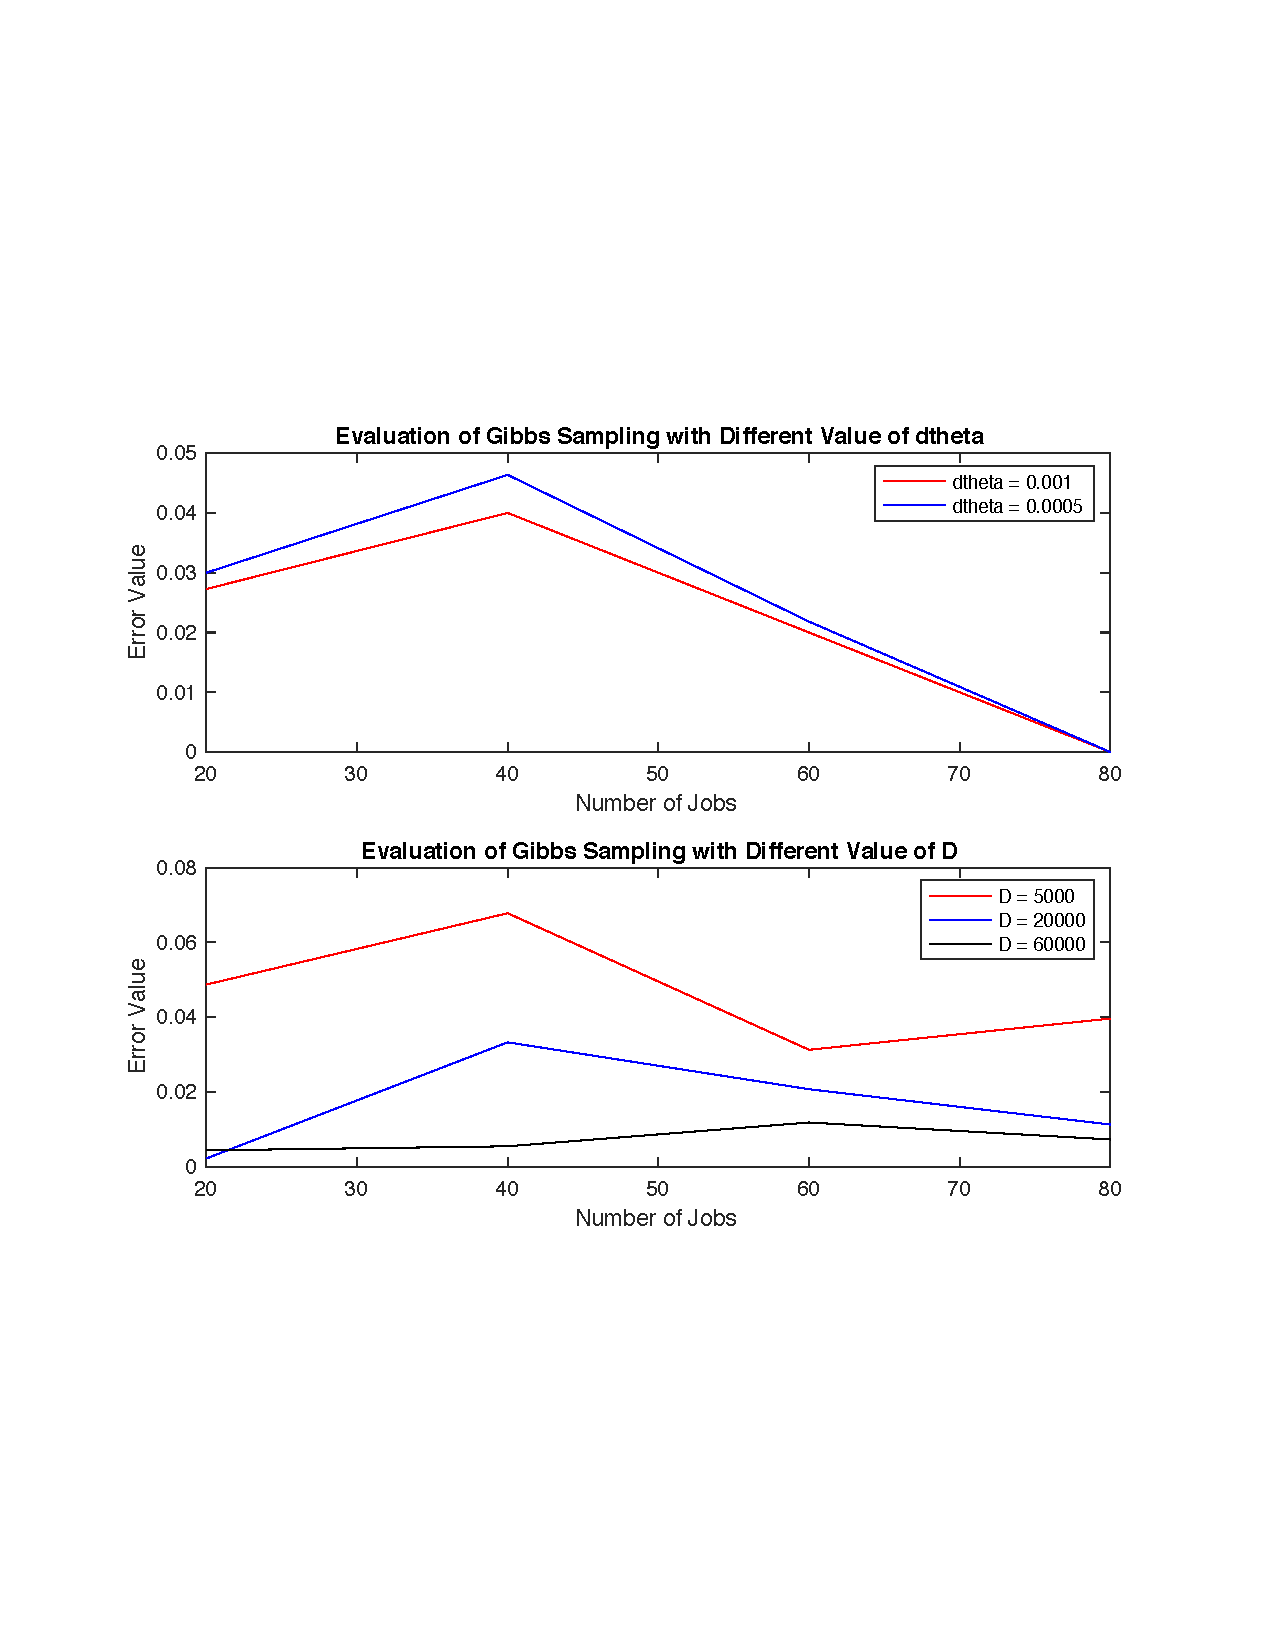
\includegraphics[width=120mm, scale=0.5]{single_class_single_station_mcmc_eval.pdf}
\caption{Evaluation of Gibbs Sampling for Single Class Queueing Network with a Single Station }
\label{fig:M1R1_eval_gibbs}
\end{center}
\end{figure}

Both graphs in Figure \ref{fig:M1R1_eval_gibbs} show a very low error value for all populations of $k$. The error value never rises above $7\%$, therefore we can conclude that for this example our Gibbs algorithm predicts the demands of the original queueing network with high precision. We have that a value of $\delta \theta = 0.01$ gives the better error metric, and the best number of samples to choose is $D = 60000$. It is not surprising that if we have a higher number of samples then we get a better error. What is interesting is that in this situation a higher step-size gives better error.

\subsubsection{Example 2: 2 Stations, 1 Class}

For this example we generate a queueing network using the demand vector given by: $\bm{\theta} = [1/60,1/40]$, where each value in $\bm{\theta}$ represents the demand of a station. The aim of our Gibbs sampling algorithm is to estimate these demands from certain parameters of the network. Figure \ref{fig:M2R1_eval_gibbs} shows the error of our algorithm when considering the different hyper-parameters that we change, similar to the case of evaluating our algorithm for the single class single station network. Again, we take the error for many different populations of jobs in the network to see how well our algorithm generalizes. \\

\begin{figure}[h!]
\begin{center}
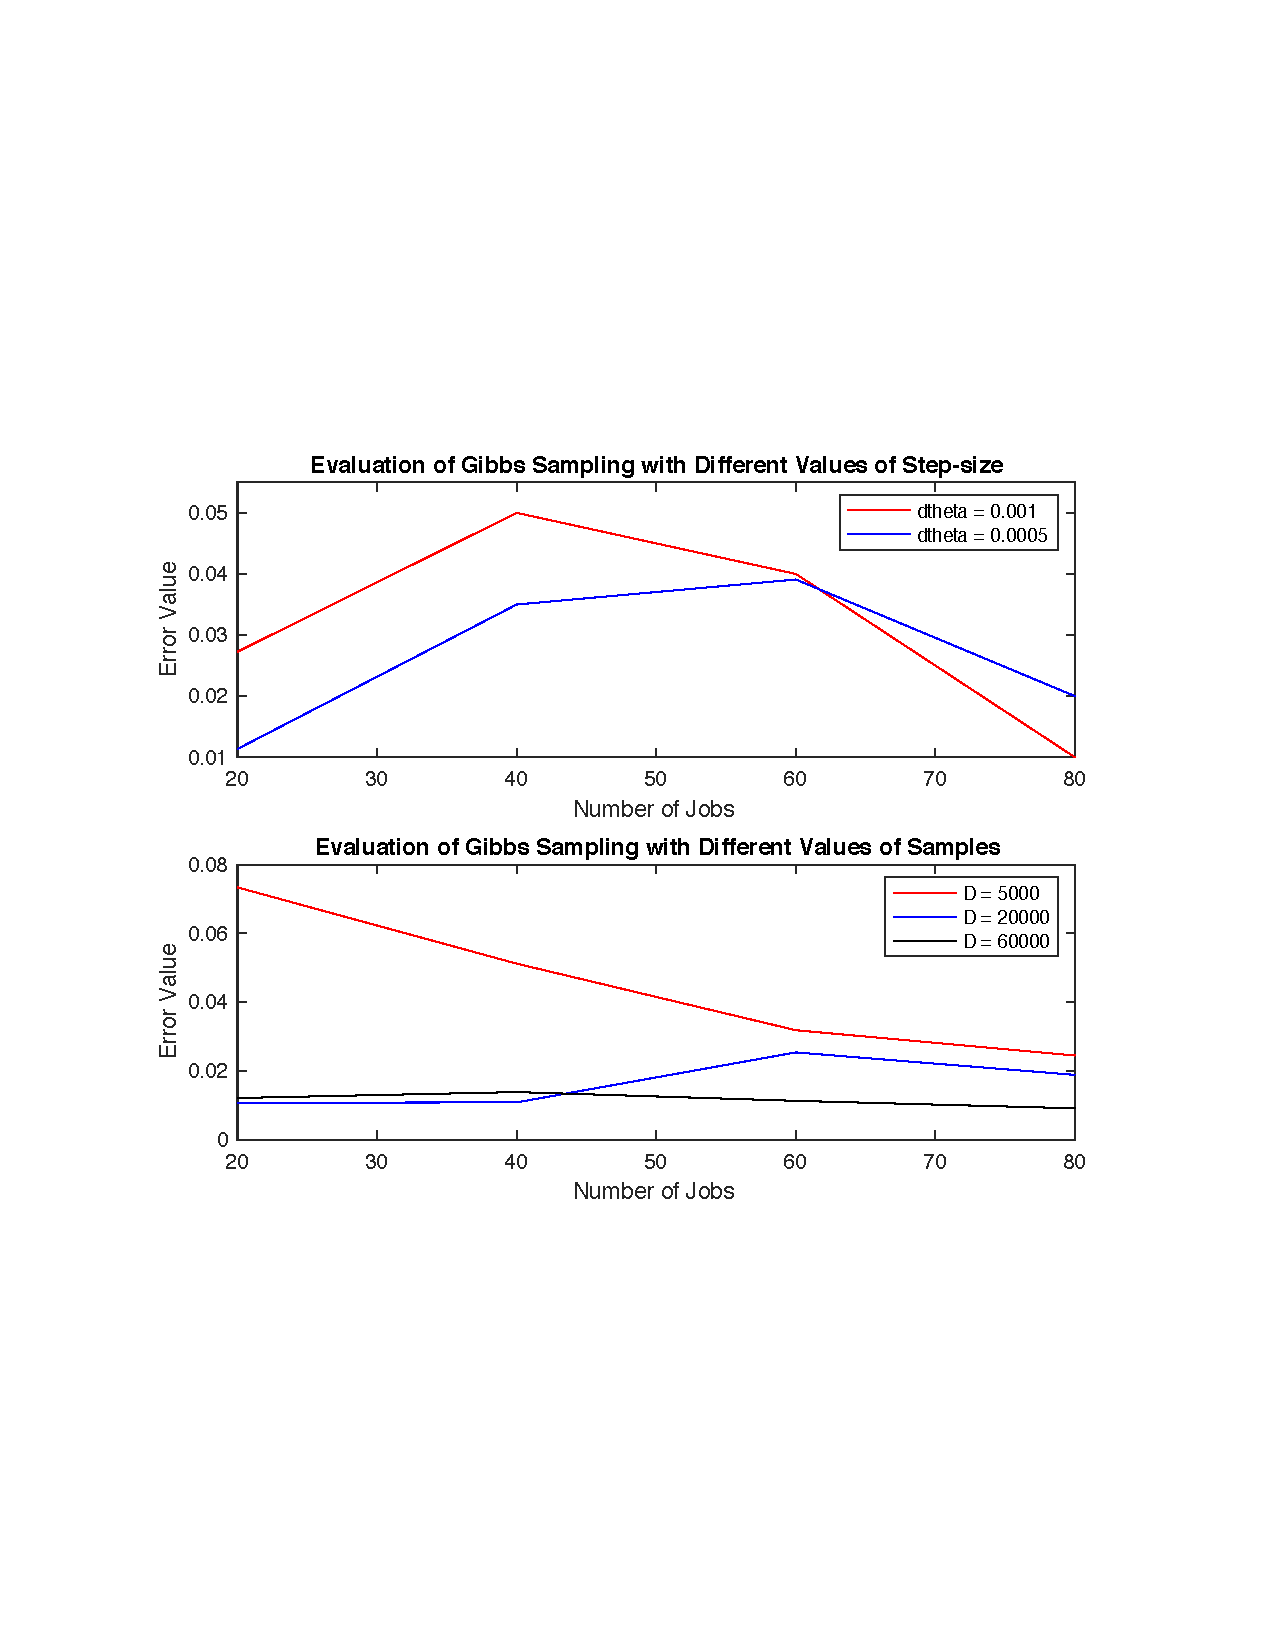
\includegraphics[width=120mm, scale=0.5]{M2R1_gibbs_eval.pdf}
\caption{Evaluation of Gibbs Sampling for Single Class Queueing Network with 2 Stations}
\label{fig:M2R1_eval_gibbs}
\end{center}
\end{figure}

In this example we have that the error is always less than $8\%$, which shows that our algorithm works well at predicting the demand estimations. For most of our hyper-parameters, we have a very good prediction. The best prediction is when we have $D = 60000$, $\delta \theta = 0.0001$, as shown by the black line in the second subplot of Figure \ref{fig:M2R1_eval_gibbs}. 

\subsubsection{Example 3: 3 Stations, 1 Class}

For this example we generate a queueing network using the demand vector given by: $\bm{\theta} = [1/60,1/40,1/50]$. Figure \ref{fig:M3R1_eval_gibbs} shows the error in demand estimation for this network. For this example, we have that the error is always below 4\% for the span of initial populations that we chose, which indicates that our algorithm worked very well in estimating the service demands. This also seems to show that the number of stations in the single class system doesn't affect the accuracy of our prediction. We have that in our single class system examples, this example with 3 stations had the best average accuracy across all hyper-parameters. All stations had good accuracy, however. 

\begin{figure}[h!]
\begin{center}
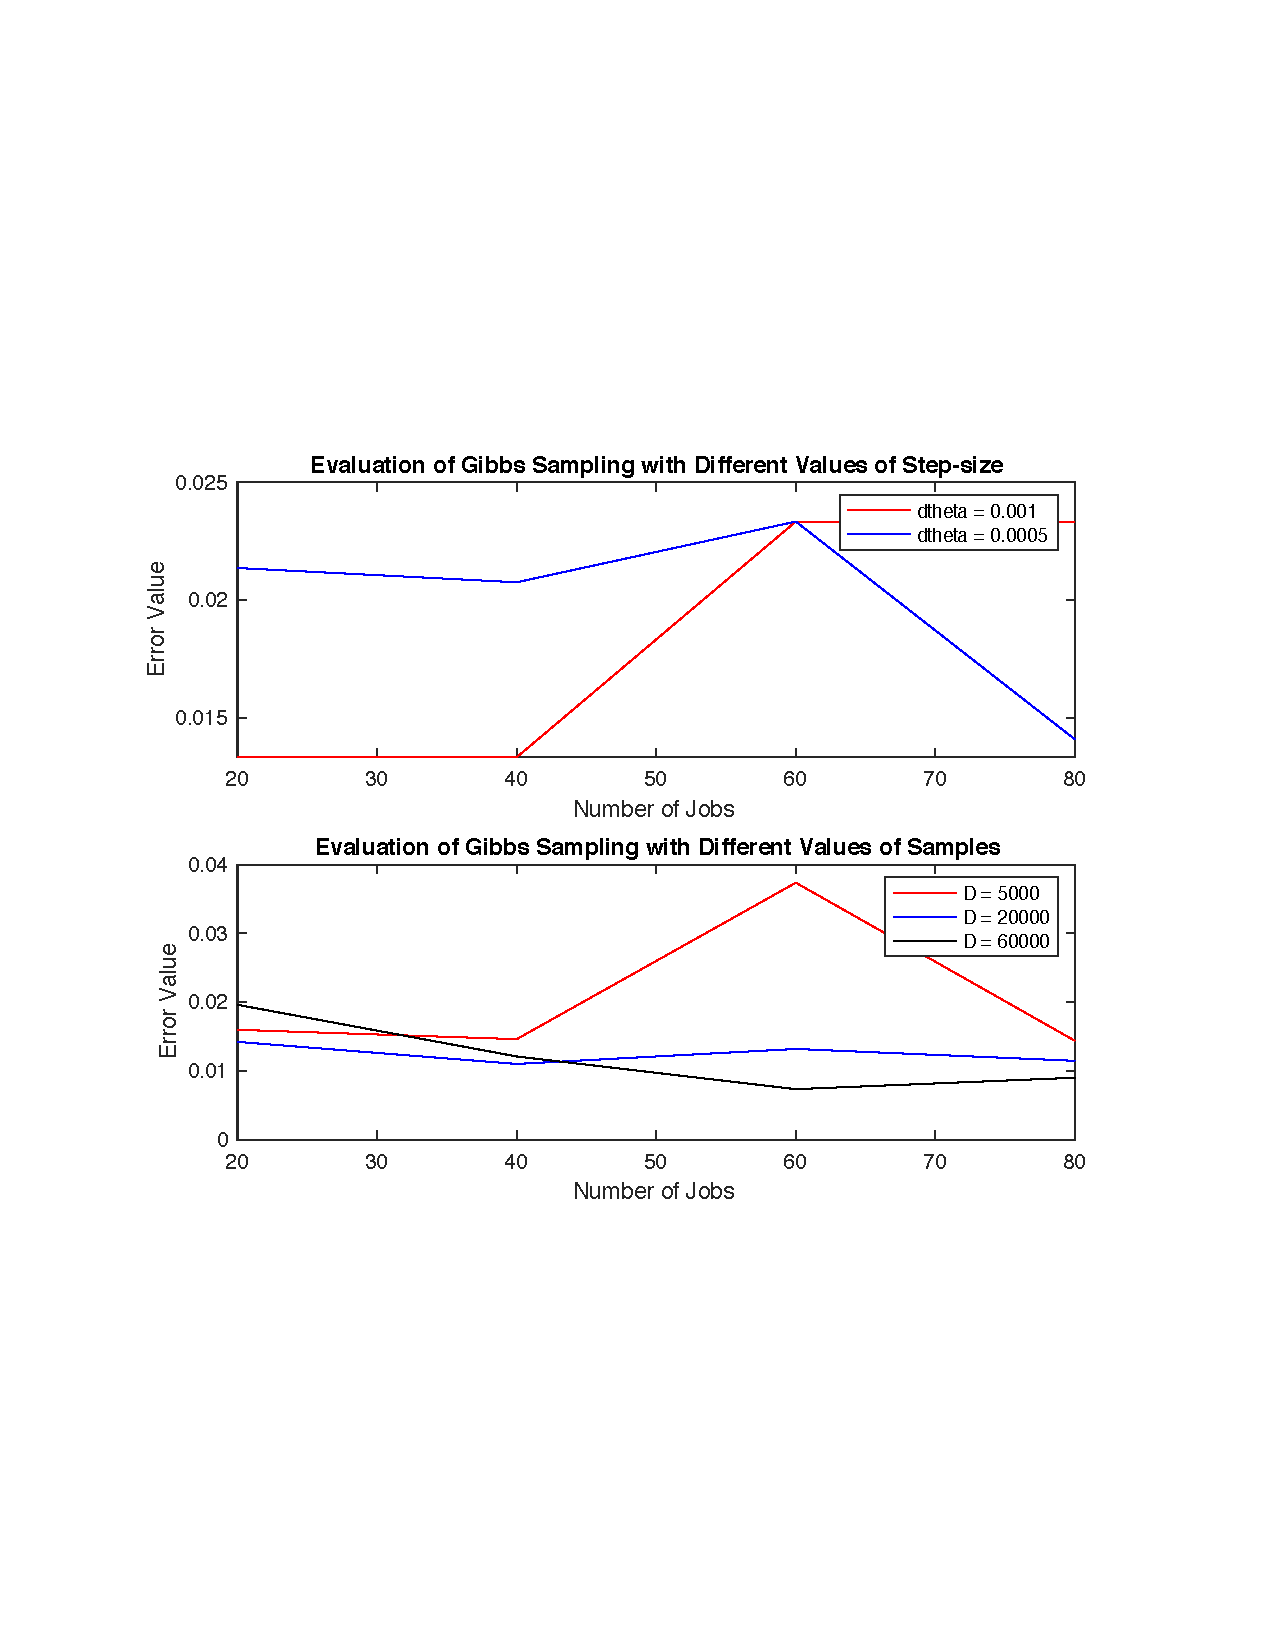
\includegraphics[width=120mm, scale=0.5]{M3R1_gibbs_eval.pdf}
\caption{Evaluation of Gibbs Sampling for Single Class Queueing Network with 3 Stations}
\label{fig:M3R1_eval_gibbs}
\end{center}
\end{figure}

\subsubsection{Example 4: 2 Stations, 2 Classes}

This example consists of a queueing network with 2 Processor Sharing nodes and 2 job classes. Figure \ref{fig:M2R2_eval_gibbs} shows the error of our models when applied to this example. \\

\begin{figure}[h!]
\begin{center}
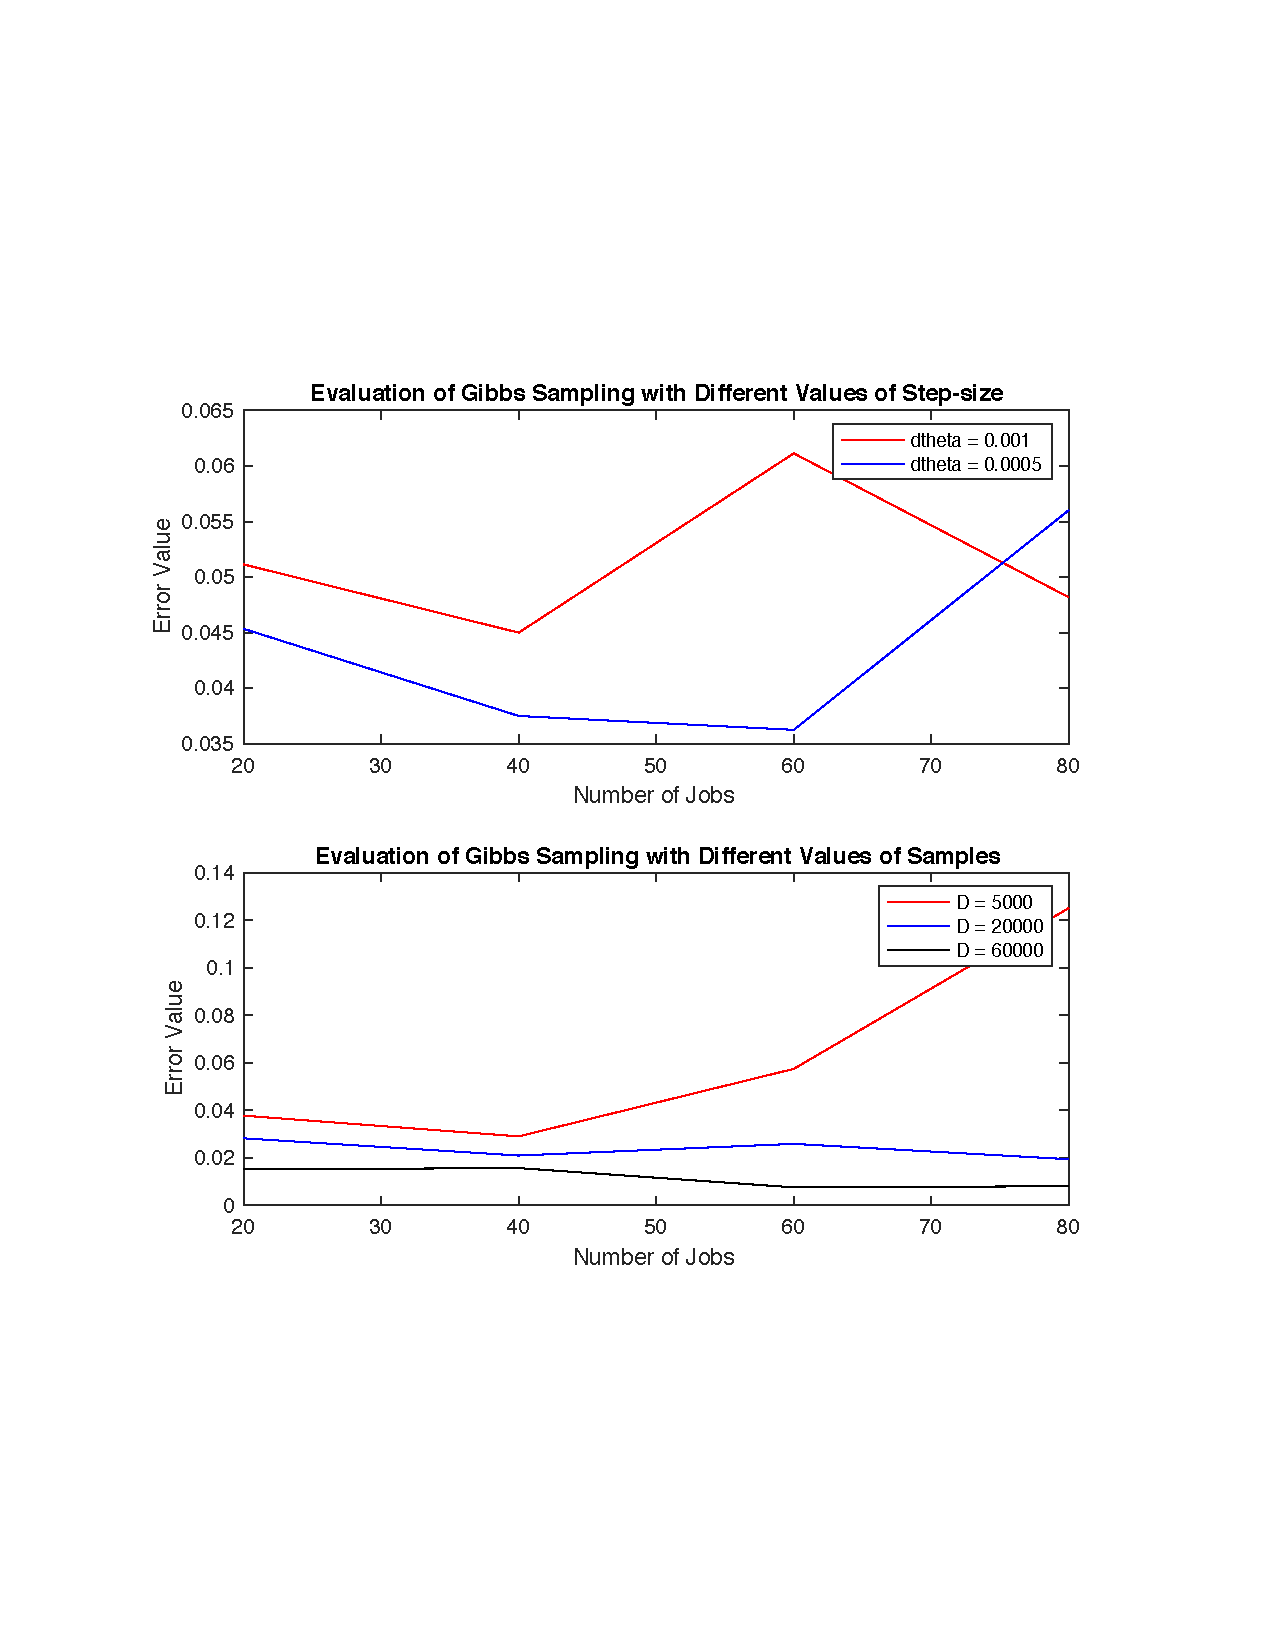
\includegraphics[width=120mm, scale=0.5]{M2R2_gibbs_eval.pdf}
\caption{Evaluation of Gibbs Sampling for Queueing Network with 2 Stations and 2 Classes}
\label{fig:M2R2_eval_gibbs}
\end{center}
\end{figure}

We have that when we choose $D = 5000$ samples, our error increases up to an alarming value of $13\%$ when the population of jobs in the network is 80, and most likely would increase further more if we tried larger values of population. This is most likely because we have not chosen enough samples to give accurate predictions when the number of jobs in the network is large. When we have $D \geq 10000$, the error of our models is very good and stays below 6.5\%. Therefore, as long as we keep the number of samples above 10000 we achieve very good results for this example. We can conclude then that our Gibbs algorithm works for simple multi-class queueing systems. 

\subsubsection{Example 5: 3 Stations, 2 Classes}

We will now examine one last example of a more complex queueing network than the previous examples. We will see how well our algorithm predicts the demands of a queueing network that has 3 stations and 2 job classes. This creates a $3 \times 2$ matrix of demands that we need to predict, which is slightly larger than the previous examples. As a result of the higher complication, we will increase the range of the number of jobs in our experiment from 80 to 100. \\

\begin{figure}[h!]
\begin{center}
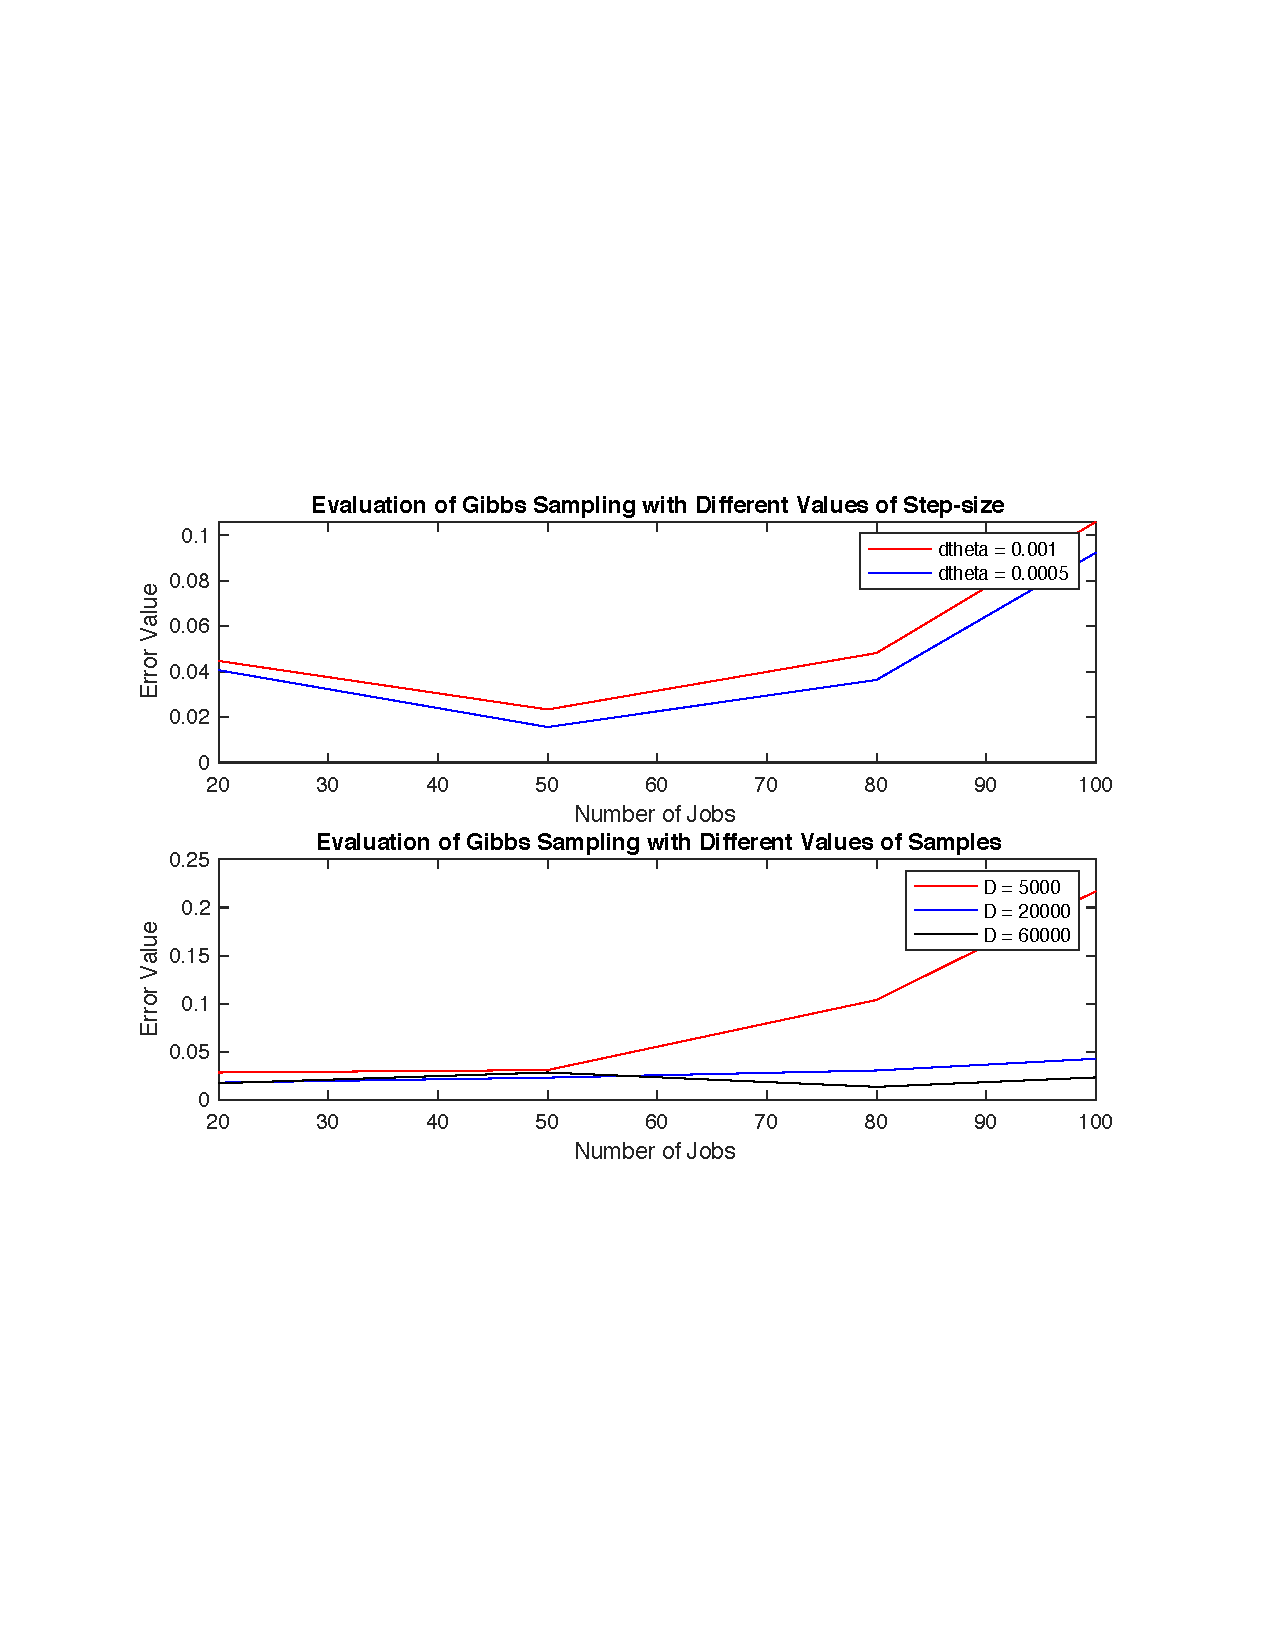
\includegraphics[width=120mm, scale=0.5]{M3R2_eval_gibbs.pdf}
\caption{Evaluation of Gibbs Sampling for Queueing Network with 3 Stations and 2 Classes}
\label{fig:M3R2_eval_gibbs}
\end{center}
\end{figure}

As can be seen from Figure \ref{fig:M3R2_eval_gibbs}, our error values are low but only when we have large sample size $D$ for the Gibbs algorithm. When we use a sample size $D \geq 20000$, our error stays below 5\% up to a population of 100 jobs in the system. When we have a sample size of $D=5000$ the error is too high when we have a high population of jobs. This is because our queueing network is too complex to be predicted using a small sample size. 

\subsection{Conclusion and Evaluation of the MCMC Method}

Overall, our Gibbs algorithm has very promising and favourable results on the chosen examples that we have used for demand estimation. In all cases, we have managed to get an error of below 5\%. From our results, there is evidence to show that the more complex our network is, the more samples are required to get an accurate prediction. Additionally, we have performed a hyper-parameter search on the step size and the number of samples to find the best set of parameters for each example, and in conclusion we have found that larger, more complex queuing networks require a larger sample size and a smaller value for the step-size. We have only examined PS queueing networks as our examples, but as seen in the references [Cas16] and [Cas13] this algorithm will give favourable results for not only other BCMP queueing networks but also other more general queueing networks. We have shown that this algorithm gives favourable results for demand estimation on both single-class and multi-class queueing networks. 

\subsection{Dirichlet Priors}

We have seen in our evaluation of the Gibbs sampling methodology that the error of our predictions for the service demands increases when we use a small sample size and we have a large population of jobs in the system. This is shown in Figure \ref{fig:M2R2_eval_gibbs} and \ref{fig:M3R2_eval_gibbs}, where the error for $D=5000$ becomes worrying when we have a high population of jobs in the system. To attempt to lower this we can use Dirichlet priors as a prior distribution in our Bayesian inference estimation instead of a uniform distribution. The prior distribution is denoted as $P(\bm{\theta})$, and is particularly useful when the size $N$ of the dataset is small or when we only choose a small number of samples for our MCMC algorithm [Cas16]. We use prior distributions to express our belief's about the system before any evidence is taken into account [Sut11].  \\

The Dirichlet distribution is the conjugate prior of the multinomial distribution [Sap17]. Since the BCMP product form is a scaled product of multinomial terms, it makes sense for the Dirichlet prior to be the natural choice as the prior distribution [Cas16]. We define the probability density function of the Dirichlet distribution of order $n$ as shown in Equation \ref{eqn:dirichlet_pdf} [Cas16], [Sap17]:

\begin{equation}
    f(\mathbf{x}; \mathbf{q}) = \frac{1}{B(\mathbf{q})} \prod_{i=1}^{n} x_{i}^{q_i-1}
    \label{eqn:dirichlet_pdf}
\end{equation}

where $\matbf{x} = (x_1,...,x_n)$ denotes the $n$ variables and $\mathbf{q} = (q_1,...,q_n)$ denotes the $n$ concentration parameters, where $q_i \geq 0$. $B(\mathbf{q})$ denotes the normalizing constant, which is defined using the gamma function $\Gamma(x)$ with a constraint that $\sum_{j=1}^n x_j = 1$ [Cas16]: 

\begin{equation}
    B(\mathbf{q}) = \frac{\prod_{i=1}^n \Gamma(q_i)}{\Gamma(\prod_{i=1}^n q_i)}
\end{equation}

The mean and variance of each variable $x_i$ in the Dirichlet distribution is given as $E[x_i] = q_i/q_0$, where $q_0 = \sum_{i}^{n} q_i$. From [Cas16] and it can be seen that using an adaptation of this Dirichlet prior instead of the uniform prior in Gibbs sampling gives a better prediction for results when the sample size is small, specifically when D $\leq$ 50. Therefore, thinking about which prior distribution to use is very important, especially in real-life scenarios where maybe we do know some prior knowledge about the data. 
% Explain Dirichlet Priors

\section{Learning Queuing Networks Using Recurrent Neural Networks}

In this section we will examine how we can use an adaptation of a recurrent neural network to predict queuing network parameters from data. The methodology of this section is based on the work by Garbi, Incerto and Tribastone [Gar20]. Our aim is to automatically learn analytic performance model parameters from data which consists of execution traces. Our approach is to have an input consisting of the shared resources of a queueing network and their concurrency levels, from which we learn the underlying topology and the service demands of the queueing network. We have that estimating the routing probabilities and service demands leads to a nonlinear optimization problem, as they serve as multiplicative factors in the dynamic equations that describe the evolution of a queueing network. We will attempt to learn the behaviour of a queueing system from execution traces by using recurrent neural networks, as these are well known for being able to fit to nonlinear systems [Sch19]. We will use an approximate and compact system of nonlinear equations to represent the dynamics of the queueing network, instead of the comparatively large exact system of equations that we usually use to describe the dynamics [Gar20]. These approximations are called fluid approximations, and they consist of only one ODE approximation per queueing station [Gar20], [Mic19]. We will use it to describe the time evolution of the queue length at each station, which describes the number of clients contending for each resource [Bol06]. The fluid approximations will determine the average queue length of the underlying stochastic process. In this section we will determine whether there is a direct association between the queuing network fluid approximation structure and the standard activation functions and layers of an RNN [Gar20]. We will train our RNN using the transient evolution of the measured average queue length at each service station. Subsequently, the learned weights of the RNN can be interpreted as a queueing network with learned parameters, such as the initial states, service demand, number of servers, and the underlying routing probabilities [Gar20]. 

\subsection{Queuing Network Notation}

Firstly, we need to mathematically define the queueing networks that we will analyse, which means we have to provide the underlying mathematical concepts of the queueing networks. We have seen how to notate and describe the functionality of queueing network parameters in Section 3.3, so here we will just define the most important aspects of the queueing network with limited explanation. Additionally, we will assume that all queueing networks that we will use in this methodology are closed and single-class. This means that the transition probability matrix $\mathbf{P}$ is a stochastic matrix, where all of the rows will have values that sum to 1. We will formally define the queueing network using the following notation [Gar20]:

\begin{itemize}
    \item N: The number of clients in the network.
    \item M: The number of stations in the network.
    \item $\mathbf{s} = (s_1,...,s_M)$: The vector of concurrency levels, which is otherwise known as the vector that denotes the number of servers at each station. For example, $s_2$ gives the number of servers at the second station. 
    \item $\bm{\mu} = (\mu_1,...,\mu_M)$: The vector of service rates. 
    \item $\mathbf{P}$: The state transition probability matrix. 
    \item $\mathbf{x}(0)$: The initial state, which denotes the number of clients initially at each service station. 
\end{itemize}

As an example to explain the mathematical theory of this approach, we will use the queueing network shown in Figure \ref{fig:RNN_queue}, which has $M=3$ stations. 

\begin{figure}[h!]
\begin{center}
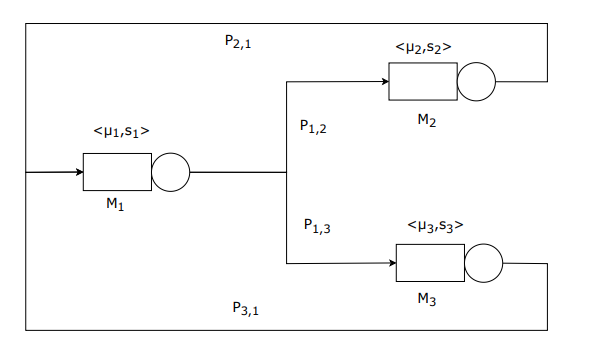
\includegraphics[width=100mm, scale=0.5]{RNN_queueing_network.png}
\caption{Queueing Network RNN (taken from [Gar20])}
\label{fig:RNN_queue}
\end{center}
\end{figure}

\subsection{Markov Chain Semantics of our Queueing Network}

Now that we have defined an example queueing network, we can analyse the mathematics behind the underlying continuous-time Markov chain that we will use to describe this network. We have discussed in previous sections how it is possible to describe a queueing network by using this technique. The reason we do this is because it makes it easier for us to predict parameters of the network when we put it into this form. We will use our CTMC representation of the queueing network to describe the probability of the queueing network having a given configuration of the queue lengths at each service station. We define a discrete CTMC state as a vector of queue lengths at each station: $\mathbf{X} = (X_1,...,X_M)$. We have that at each station $i$, if $X_i \leq s_i$ then these jobs are processed in parallel each with a rate of $\mu_i$. Additionally, if $X_i > s_i$, then we have that the total number of jobs that are queueing for the service is $X_i - s_i$ [Gar20]. We have that when one job is serviced at a station $i$, it has a probability $p_{ij}$ that the job will move from service station $i$ to service station $j$ to receive further service. We can formalize this in a way that is easy to visualize by describing the CTMC transitions by using jump vectors and their associated transition functions from an arbitrary state $\mathbf{X}$ [Bor13]. \\

We use jump vectors notated by $h^{(ij)}$ to define the state updates of our Markov chain when a job moves from station $i$ to station $j$ after being serviced at station $i$. We can define $q(\mathbf{X}, \mathbf{X}+h^{(ij)})$ to be the transition rate from state $\mathbf{X}$ to state $\mathbf{X} + h^{(ij)}$. Equation \ref{eqn:jumpvectorstates} shows the transition rates when using jump vectors [Gar20]: 

\begin{equation}
    \mathbf{X}+h^{(ij)} = \left(X_1,...,X_i-1,...,X_j+1,...X_M \right)
    \label{eqn:jumpvectorstates}
\end{equation}

where the number of jobs at station $i$ is decreased by 1 and the number of jobs at station $j$ is increased by 1. We can then fully define the CTMC as follows [Gar20]: 

\begin{equation}
    q(\mathbf{X},\mathbf{X}+h^{(ij)}) = \mathbf{P}_{i,j} \mu_i \text{min}(X_i,s_i)
    \label{eqn:CTMC_NN}
\end{equation}

where $i,j = 1,2,...,M$. To explain this further we will take the example shown in Figure \ref{fig:RNN_queue} [Gar20], where we have $M=3$ stations. We consider the same example as detailed in [Gar20]. For this example, we have the following jump vectors: 

\begin{align}
    h^{(1,2)} &= (-1,1,0)  & h^{(1,3)} &= (-1,0,1) \\
    h^{(2,1)} &= (1,-1,0)  & h^{(3,1)} &= (1,0,-1)
    \label{eqn:example_jump_equations}
\end{align}

The corresponding transitions are notated as follows: 

\begin{align}
    q(\mathbf{X},\mathbf{X}+h^{(1,2)}) = \mathbf{P}_{1,2} \mu_1 \text{min} (X_1,s_1) \\
    q(\mathbf{X},\mathbf{X}+h^{(1,3)}) = \mathbf{P}_{1,3} \mu_1 \text{min} (X_1,s_1) \\
    q(\mathbf{X},\mathbf{X}+h^{(2,1)}) = \mathbf{P}_{2,1} \mu_2 \text{min} (X_2,s_2) \\
    q(\mathbf{X},\mathbf{X}+h^{(3,1)}) = \mathbf{P}_{3,1} \mu_3 \text{min} (X_3,s_3) 
\end{align}

We have that a CTMC is completely described by the transitions shown in Equation \ref{eqn:CTMC_NN} and an initial state vector $\mathbf{x}(0)$ [Gar20]. The main issues that we will face with this representation of the CTMC is that the exact equations to analyze the probability distribution grow combinatorially with the number of jobs and the number of stations [Gar20]. 

\subsection{Fluid Approximations}

Fluid approximations can be a very useful tool for both a transient and steady-state analysis of closed queueing networks [Zhu20], and mixed multi-class queueing networks [Ngu93]. In this section, we will provide the mathematical concepts that we will need when using fluid approximation equations within our recurrent neural network model. The fluid approximation of a single-class queueing network consists of an ODE system whose size is equal to the number of stations in the queueing network, which is denoted by $M$. In this methodology, we use fluid approximations to approximate the equations of the underlying CTMC of our queueing network. Fluid approximations are known to have seen great success in approximating the macro-scale behaviour of Markov systems with a large number of discrete states [Mic19]. We let the ODE system be built by using the average impact that each transition has on the queue length at each station $k$ [Gar20]. We obtain this by calculating the product of the jump vector at the $k$th station, denoted by $h_k^{(ij)}$ and the function for the associated transition rate $q(\mathbf{X}, \mathbf{X}+h_k^{(ij)})$. We choose the variables of the fluid approximation to be $\mathbf{x} = (x_1,...,x_M)$. Subsequently, the corresponding ODE system is given by [Gar20]: 

\begin{equation}
    \frac{d x_k(t)}{dt} = \sum_{h^{(ij)}} h_k^{(ij)} q(\mathbf{x}(t), \mathbf{x}(t)+h^{(ij)})
    \label{eqn:ODE_system}
\end{equation}

where $k = 1,...,M$. We interpret the solution for each coordinate $x_k(t)$ as an approximation of the average queue length as given by the CTMC semantics at time $t$ [Bor13]. Additionally, we have that when the number of jobs and stations in the system are large enough, the approximation and the exact equations of the CTMC become indistinguishable from one another [Kur70]. Equation \ref{eqn:ODE_system} can be formalised using Equation \ref{eqn:CTMC_NN} as follows [Gar20]: 

\begin{equation}
    \frac{d x_k(t)}{dt} = \sum_{i \neq k} \mathbf{P}_{i,k} \bm{\mu}_i \text{min} (\mathbf{x}_i (t), s_i) + ( \mathbf{P}_{k,k} -1) \bm{\mu}_k \text{min} (\mathbf{x}_k (t), s_k)
\end{equation}

where we include the term $\mathbf{P}_{k,k}$ as the self loops in the system. If we consider the running example that we have, shown in Figure \ref{fig:RNN_queue}, then we get the following fluid approximation equations [Gar20]: 

\begin{align}
    \frac{d x_1(t)}{dt} &= -\bm{\mu}_1 \text{min}(\mathbf{x}_1 (t), s_1) + \bm{\mu}_2 \text{min}(\mathbf{x}_2 (t), s_2) + \bm{\mu}_3 \text{min} (\mathbf{x}_3 (t), s_3) \\
    \frac{d x_2(t)}{dt} &= -\bm{\mu}_2 \text{min}(\mathbf{x}_2 (t), s_2) + \mathbf{P}_{1,2} \bm{\mu}_1 \text{min}(\mathbf{x}_1 (t), s_1) \\
    \frac{d x_3(t)}{dt} &= -\bm{\mu}_3 \text{min}(\mathbf{x}_3 (t), s_3) + \mathbf{P}_{1,3} \bm{\mu}_1 \text{min}(\mathbf{x}_1 (t), s_1)
\end{align}

From the queue length estimates, we can find other important performance metrics of a queueing network such as the throughput, response time and utilization as detailed in Section 3.3.2. One drawback of using the fluid approximation is that for a queueing network with self loops there will exist another one without self loops that we will not be able to distinguish [Gar20]. A network without self loops is a network such that $\mathbf{P}_{k,k} = 0$ for $k = 1,...,M$. Therefore, we will focus our RNN on queueing networks that do not have self loops.

\subsection{Method of Machine Learning}

We will be learning the architecture of the underlying CTMC of a queueing network by using RNNs. We therefore need to develop a suitable RNN architecture to learn this information. Our method of machine learning will attempt to encode the queueing network dynamics in a fashion that we can interpret, where we associate the weights of the queueing network with parameters such as routing probabilities, service rates and concurrency values [Gar20]. We can split our method of machine learning into 4 steps. Firstly, we need to obtain an ODE discretization of the underlying fluid approximation of the queueing network such that we can assign a layer of the RNN to each time step of the discretization. Secondly we decide a fashion in which we can encode the RNN. Thirdly, we determine what kind of input data we need for our model. Finally, we determine a suitable loss function that we will use for our model. We will now discuss these steps in further detail.

\subsubsection{ODE Discretization of Fluid Approximation}

For a given queueing network, the associated fluid approximation is detailed by Equation \ref{eqn:fluid_approximation} [Mic19].

\begin{equation}
    \frac{d x(t)}{dt} = - \bm{\mu} \text{min} (x(t), s) + \mathbf{P}^T \bm{\mu} \text{min} (x(t),s)
    \label{eqn:fluid_approximation}
\end{equation}

where $x(t)$ denotes the mean queue lengths at time t, which is an M-dimensional vector. To use this Equation \ref{eqn:fluid_approximation} in our model we need to find a time-discrete version of it, where when we consider small time steps denoted by $\Delta t$ we obtain: 

\begin{equation}
    x(t + \Delta t) = x(t) + \Delta t (-\bm{\mu} \text{min} (x(t), s) + \bm{\mu} \mathbf{P} \text{min}(x(t),s))
    \label{time_discrete_fa}
\end{equation}

which we can write as [Gar20]: 

\begin{equation}
    x(t + \Delta t) = x(t) + \Delta t \mathbf{u}(t) (\bm{\mu} \odot (\mathbf{P} - \mathbf{I})).
    \label{time_discrete_fa_odot}
\end{equation}

where we define $\mathbf{u}(t)$ as $\text{min} (x(t),s)$ and $\odot$ as the mathematical operator which has the following indication: if $\mathbf{C} = \mathbf{a} \odot \mathbf{B}$, then $\mathbf{C}_{i,j} = \mathbf{a}_i . \mathbf{B}_{i,j}$. 

\subsubsection{RNN Encoding}

We can take the discretization as detailed by Equation \ref{time_discrete_fa_odot} as a direct encoding of the RNN [Gar20]. We define an input layer $\hat{x}_0$ which denotes the M-dimensional initial input. Our RNN will have $H-1$ cells, where the $h$th cell attempts to compute the estimate of the queue length at time $h \Delta t$, and is denoted as $\hat{x}_h$. We use the $h$th cell to compute the following equation: $\hat{x}_h = \hat{x}_{h-1} + \Delta t \hat{u}_{h-1} (\bm{\mu} \odot (\mathbf{P}-\mathbf{I}))$. Additionally, we have that $\hat{u}_{h-1}$ is an estimation of $\mathbf{u}((h-1)\Delta t)$. We then have that our aim is to learn the matrix $\mathbf{P}$, which consists of $M(M-1)$ weights as we are assuming that the diagonal is empty due to their being no self loops in the system, and the vector $\bm{\mu}$ which is made up of $M$ weights. The ultimate aim of this method is to learn the parameters of the queueing network. To make this simpler, we can enforce some constraints on our model. We will assume that $\mathbf{P}$ is a stochastic matrix, that there is an absence of self loops in the system such that the diagonal values of the matrix $\mathbf{P}$ are set to zero, and $\bm{\mu} \geq 0$. We enforce these constraints in the following ways: the weights are ensured to be non-negative by fixing the candidate values within the range $[0,\infty)$; we ensure the matrix $\mathbf{P}$ is stochastic by dividing each weight by the sum of the weights in the corresponding row; and we enforce no self loops by setting all the values in the diagonal of the matrix $\mathbf{P}$ equal to 0 [Gar20]. \\

Therefore, the method of machine learning that we will use in this chapter lies in the explainable machine learning research area [Mol19], which therefore lets us to view each learned learned parameter and understand its role in the system. \\

If we take the example as shown in Figure \ref{fig:RNN_queue}, then we can work out the RNN encoding for the $h$th cell by computing the separate $\hat{u}_h$ vectors and the $\hat{x}_h$ vectors, shown in equations \ref{eqn:u_rnn} - \ref{eqn:x_rnn} respectively [Gar20].

\begin{align}
    \label{eqn:u_rnn}
    \hat{u}_{h-1,1} &= \text{max} (s_1, \hat{x}_{h-1,1}) \\
    \hat{u}_{h-1,2} &= \text{max} (s_2, \hat{x}_{h-1,2}) \\
    \hat{u}_{h-1,3} &= \text{max} (s_3, \hat{x}_{h-1,3})
\end{align}


\begin{align}
\hat{x}_{h,1} &= \hat{x}_{h-1,1} + \Delta t (- \bm{\mu}_1 \mathbf{\hat{u}}_{h-1,1} + \bm{\mu}_2 \mathbf{P}_{2,1} \mathbf{\hat{u}}_{h-1,2} + \bm{\mu}_3 \mathbf{P}_{3,1} \mathbf{\hat{u}}_{h-1,3}) \\
\hat{x}_{h,2} &= \hat{x}_{h-1,2} + \Delta t ( \bm{\mu}_1 \mathbf{P}_{1,2} \mathbf{\hat{u}}_{h-1,1} - \bm{\mu}_2 \mathbf{\hat{u}}_{h-1,2} + \bm{\mu}_3 \mathbf{P}_{3,2} \mathbf{\hat{u}}_{h-1,3}) \\
\hat{x}_{h,3} &= \hat{x}_{h-1,3} + \Delta t ( \bm{\mu}_1 \mathbf{P}_{1,3} \mathbf{\hat{u}}_{h-1,1} + \bm{\mu}_2 \mathbf{P}_{2,3} \mathbf{\hat{u}}_{h-1,2} - \bm{\mu}_3 \mathbf{\hat{u}}_{h-1,3})
\label{eqn:x_rnn}
\end{align}

\subsubsection{Input Data} 

Our RNN will learn by using a set of H dimensional input traces, in a similar fashion to how we used input traces to predict aspects of a queueing network in the EM algorithm. The traces are denoted as: $\hat{\tau_0},...,\hat{\tau}_{H-1}$, and the $i$th component of the $\hat{\tau}_h$ vector denotes a sample of the queue length of each station $i$ at time $t$ [Gar20]. We have that each trace used during the learning process consists of `measurements averaged over a number of independent executions that begin with the same initial condition' [Gar20]. 

\subsubsection{Error Function}

The error function of our RNN will attempt to minimize the error between the measured traces denoted by $\hat{\bm{\tau}}_h$ and the predicted queue lengths denoted by $\hat{\mathbf{x}}_h$. We will use an error function determined by the maximum relative error [Buz79], where we use the L1 Norm in our definition of the loss:

\begin{equation}
    err = \max_{h=1}^{H-1} \lVert \hat{\bm{\tau}}_h - \hat{\mathbf{x}}_h\rVert . \frac{100}{2N}
    \label{eqn:loss_function}
\end{equation}

where the loss is computing the number of jobs that are misplaced by our prediction [Gar20]. 

\subsection{Numerical Simulation - Synthetic Cases}

In this section we will explore how to use our machine learning methodology to predict aspects of synthetically generated queueing networks. We will build 3 queueing networks which have different amounts of stations, denoted by $M$; server concurrency levels, denoted by the vector $\mathbf{s}$; routing probability matrices, denoted by $\mathbf{P}$; and service rates denoted by the vector $\bm{\mu}$. For each network, we generate 100 traces which consist of the average queueing length at each station of the network over the time interval $ I = [0s,10s]$. The aim of our RNN is to predict the routing probability matrix $\mathbf{P}$ and the service rates $\bm{\mu}$ of each network from the traces. We split the traces such that half are used for training our network and half are used for validation such that we can see the validation accuracy and the validation loss during training. We set an Early Stopping condition, such that when the error computed on the validation set does not improve by at least $0.01$\% over the previous 50 epochs then we stop the training, as suggested by [Gar20]. \\ 

Our RNN will then attempt to learn the parameters of the queueing network over a set of traces. The traces are initialized with different initial populations of jobs in each station - therefore the RNN is not trying to predict the initial conditions but instead learn the queueing network parameters such that we can assign any initial conditions to the network and it will still have a good prediction of the network parameters. The RNN will predict the parameters $\mathbf{P}$ and $\bm{\mu}$ of the network. We create separate models for each queueing network that we aim to learn. 

\section{Experimental Validation of our RNN Methodology for QN Parameter Fitting}

We can evaluate our machine learning methodology by comparing the traces from the original queueing network that generated the learning traces and the traces from the learned queueing network. The generated queueing network is `unseen' as we change the server concurrency values and the initial population values. We then evaluate the predicted network against this new network by using the same values. We will also look at different performance metrics of the generated and learned queueing networks and see how they compare. The most important metric is the error in our model, which measures the average difference in the amount of jobs that are misplaced between our predicted and generated networks over time. In this section we will explain the different examples of queueing networks that we have predicted, as well as evaluate the quality of our predicted model by comparing performance metrics. In this section we will look at 3 examples of our RNN-algorithm applied to queueing networks. We will attempt to predict the parameters of the following queueing networks: a network with 3 stations; a network with 5 stations; and a network with 10 stations. We will then analyse the quality of our prediction by comparing the evolution of the following metrics over time: the average queue length, the utilization, and the absolute difference in average queue length. We will also report on the accuracy of our model. For each queueing network that we create we will generated 100 traces with different initial populations of jobs in each node. Then, we will train our model to predict the parameters of the queueing network that generated these traces. Afterwards, we will compare our predicted queueing network to an unseen generated network by using new server concurrency values and initial population of nodes. Within our validation we will create an example of each network that we predict and report on the accuracy of our prediction on that network. For all of the following examples, the RNN-methodology was implemented using the Keras framework [Cho15] with the TensorFlow backend [Aba15]. We use the `Adam' optimizer [Kin15], and a learning rate of 0.05.

\subsection{Queuing Network with 3 Stations}

In this synthetic example we create traces using a queueing network with 3 stations, therefore $M=3$. For training our model, we set the server concurrency values to $\mathbf{s} = [40, 20, 10]$; the service rates as $\bm{\mu} = [100,50,50]$; and the initial population is randomly generated for each station and trace. We set the transition probability matrix of the generating queueing network as follows: 

\begin{equation}
    \mathbf{P} = \begin{bmatrix}
     0 & 2/3 & 1/3 \\
     1/3 & 0 & 2/3 \\
     2/3 & 1/3 & 0
    \end{bmatrix}
\end{equation}

where each row in $\mathbf{P}$ sums to 1 due to the stochasticity of the matrix, and there are no self-loops in the system. We then put the traces of the average queue lengths of each station over time through our RNN algorithm, which gives us a predicted model. Subsequently, we evaluate our model by using server concurrency values of $\mathbf{s} = [50, 20,  10]$ and initial population values of $ \mathbf{x}_0 = [200,0,0]$. We can then see how the generated and predicted networks compare. \\

For this generated queueing network, we have that the predicted network has the following parameters: 

$$ \bm{\mu} = [98.6, 38.1, 51.38] $$

$$\mathbf{P} = \begin{bmatrix}
0 & 0.65 & 0.35\\
0.10 & 0 & 0.90\\
0.998 & 0.002 & 0
\end{bmatrix} $$ \\

therefore, we have that the parameters are slightly different to those in the generated queueing network. Even though these parameters are different, it does not necessarily mean that the predicted queueing network will behave in a significantly different manner. We will now explore the performance metrics of the generated and predicted queueing networks and see how they compare. We will consider the metrics: average queue length, utilization, accuracy and absolute difference in average queue length. We will not consider the metric throughput as this is determined by the service rates, which is not a suitable consideration for the quality of our predictions. \\

\textbf{Average Queue Length}: Figure \ref{fig:av_q_len_3_stations} shows the evolution of the average queue length of both the generated and the predicted queueing networks. The generated network is shown by the blue line. The predicted network is shown by the red line. We can see that in general the evolution of the average queueing length of each station behaves very similarly for both queueing networks. There is a slight discrepancy at each station, however the average queue length in the predicted network does somewhat converge to the same values as that of the generated network, and also has similar oscillations.

\begin{figure}[h!]
\begin{center}
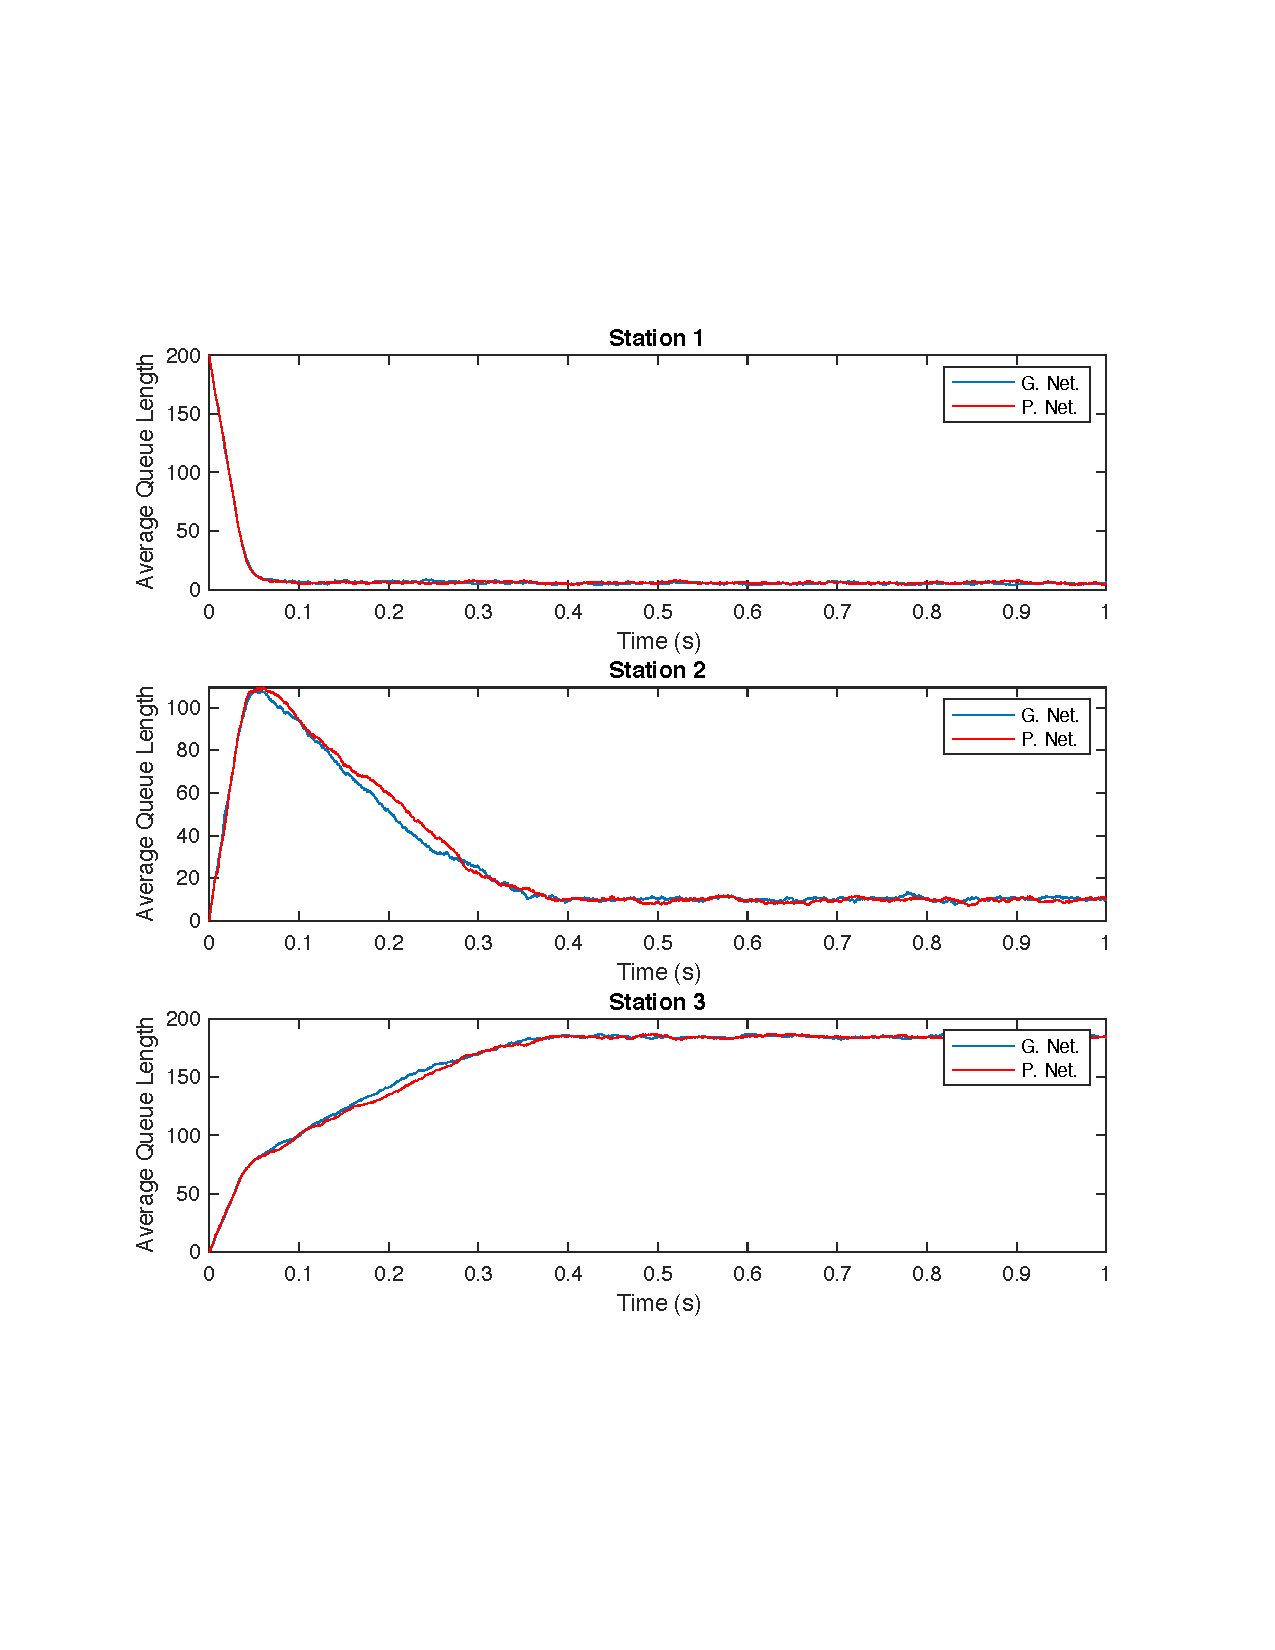
\includegraphics[width=\linewidth, scale=0.5]{av_q_len_3_stations.pdf}
\caption{Average queue length of predicted and generated networks with 3 stations}
\label{fig:av_q_len_3_stations}
\end{center}
\end{figure}

From Figure 12, we can see that our RNN-generated network predicts the average queue length evolution of the original network very well. \\

\textbf{Utilization}: Figure \ref{fig:utilization_3_stations} shows the evolution of the utilization at each station of the generated and predicted queueing networks. Similarly to the average queue length, the RNN-generated network predicts the utilization very well. The utilization settles around the same value at every station for both networks, and after the same amount of time. Additionally, the oscillations in both are fairly similar. \\

\begin{figure}[h!]
\begin{center}
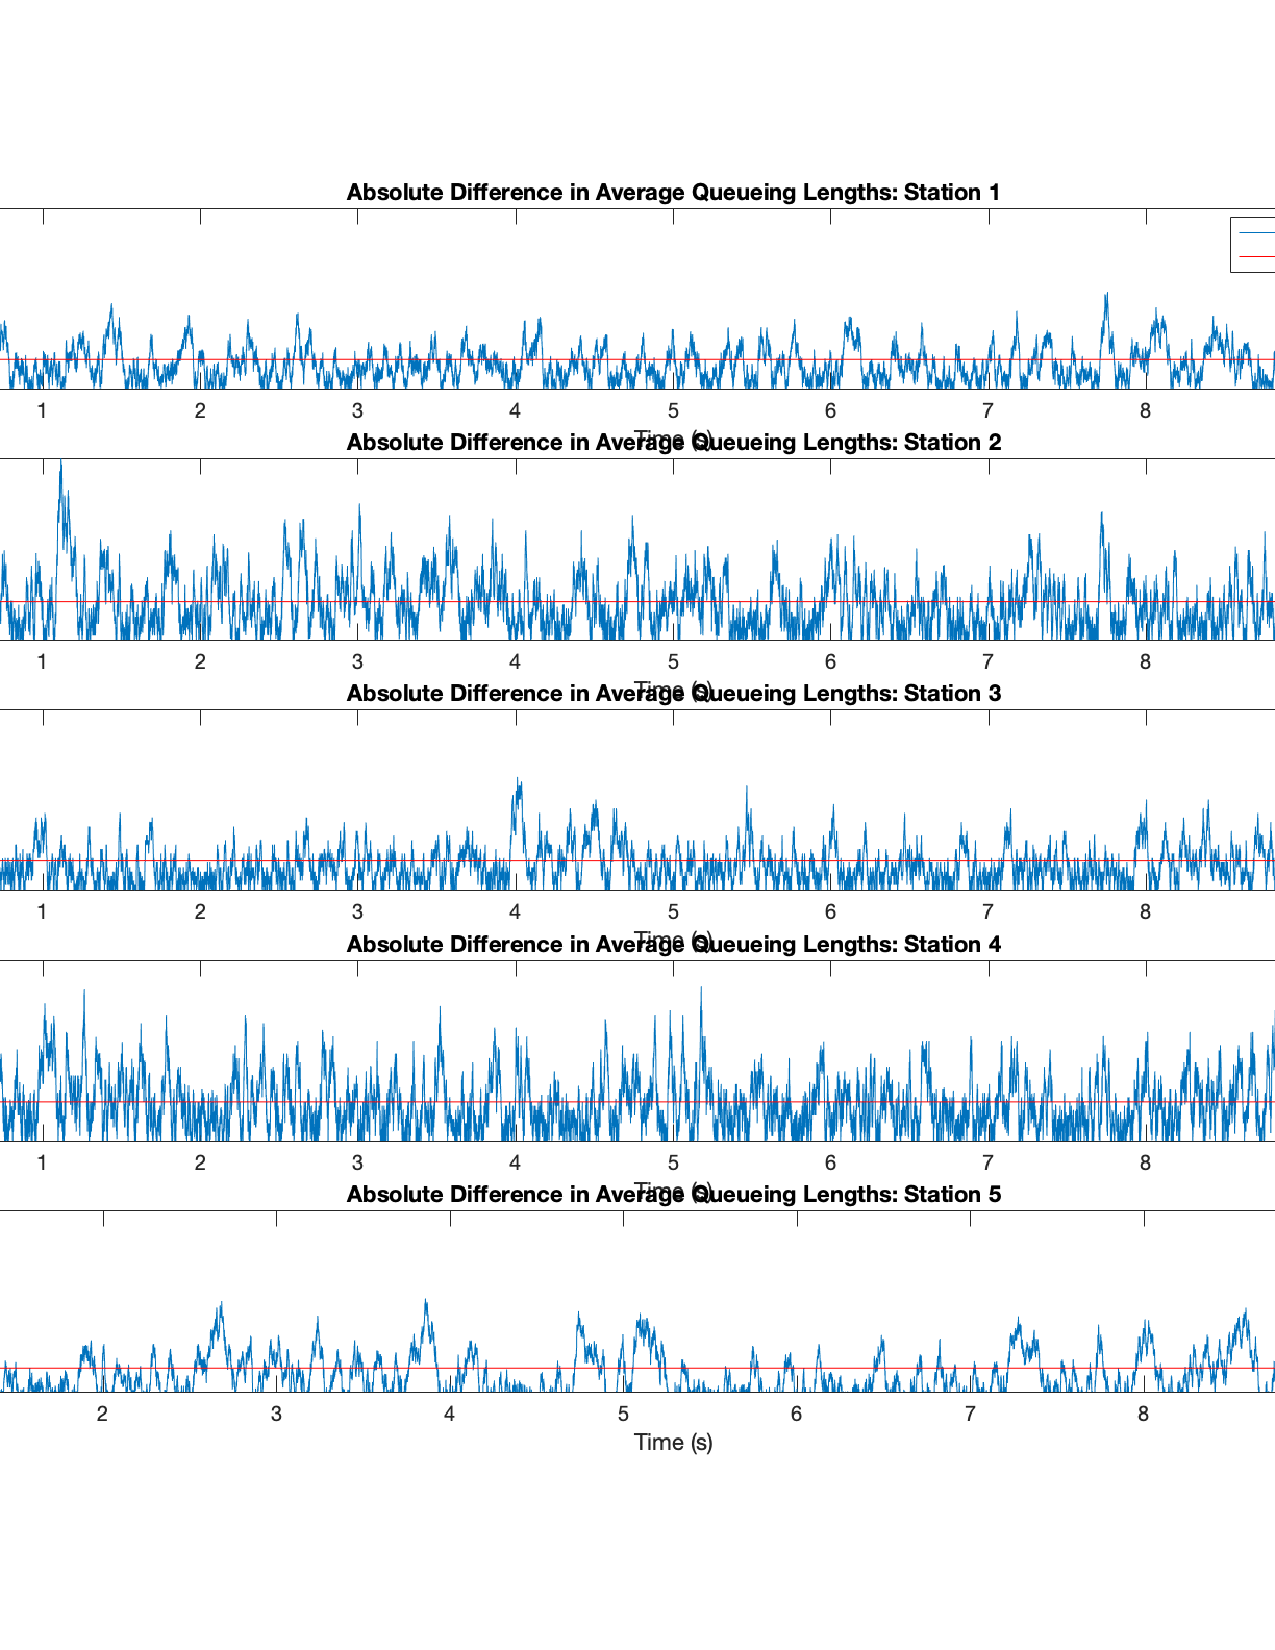
\includegraphics[width=140mm, scale=0.5]{utilization_3_stations.pdf}
\caption{Utilization of predicted and generated networks with 3 stations}
\label{fig:utilization_3_stations}
\end{center}
\end{figure}

\textbf{Error Value and Absolute Difference in Average Queue Length}: Figure \ref{fig:abs_diff_queue} shows the absolute difference in average queue length for each station. This is a very important metric as it tells us the errors in our predicted queueing network. The red line in each subplot represents the average difference in average queue length between the generating network and the predicting network. On average, at station 1 we have that 1 job is misplaced; at station 2 we have that 2 jobs are misplaced; and at station 3 we have that 2 jobs are misplaced. Additionally, we have that the error of jobs misplaced in our predicting network is 5.44\%. 

\begin{figure}[h!]
\begin{center}
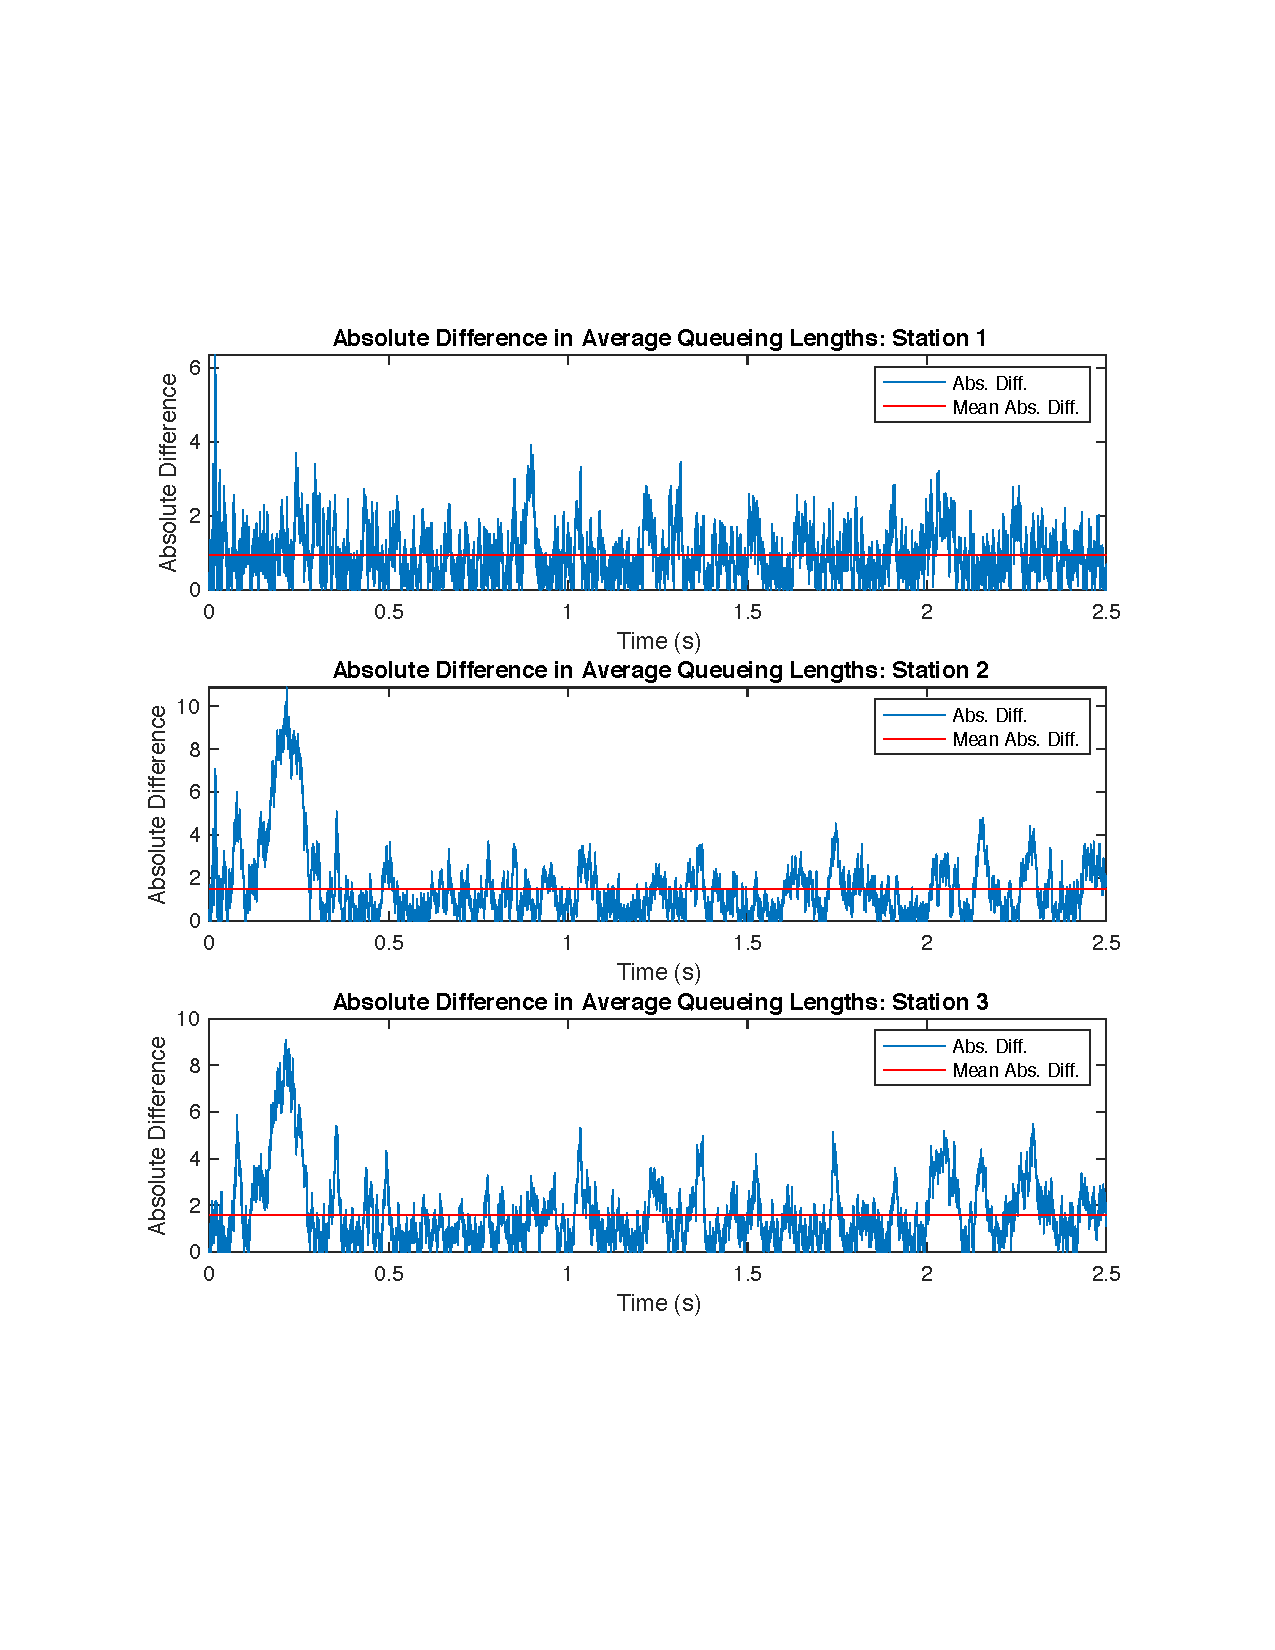
\includegraphics[width=140mm, scale=0.5]{abs_diff_3_stations.pdf}
\caption{Absolute Difference In Average Queue Length for Each Station: $err = 5.44\%$}
\label{fig:abs_diff_queue}
\end{center}
\end{figure}

\subsection{Queueing Network with 5 Stations}

We will now use an example to show the quality with which our RNN model predicts the dynamics of a queueing network that has 5 stations. In this synthetic example we create traces using a queueing network where $M=5$. For training our model, we set the server concurrency values to $\mathbf{s} = [250, 150, 80,50,20]$; the service rates as $\bm{\mu} = [50,40,30,20,10]$; and the initial population is randomly generated for each station and trace. We set the transition probability matrix of the generating queueing network as follows: 

$$\mathbf{P} = \begin{bmatrix}
0 & 0.2 & 0.2 & 0.1 & 0.5\\
0.2 & 0 & 0.1 & 0.5 & 0.2\\
0.2 & 0.4 & 0 & 0.2 & 0.2\\
0.4 & 0.2 & 0.1 & 0 & 0.3\\
0.3 & 0.2 & 0.1 & 0.4 & 0
\end{bmatrix} $$

where each row in $\mathbf{P}$ sums to 1 due to the stochasticity of the matrix, and there are no self-loops in the system. We then put the traces of the average queue lengths of each station over time through our RNN algorithm, which gives us a predicted model. Subsequently, we evaluate our model by using server concurrency values of $\mathbf{s} = [200, 100, 50,20,10]$ and initial population values of $ \mathbf{x}_0 = [150,0,0,0,0]$. We can then see how the generated and predicted networks compare. For this generated queueing network, we have that the predicted network has the following parameters: 

$$ \bm{\mu} = [8.827,13.0608,9.28407,10.970014,14.628479] $$

$$\mathbf{P} = \begin{bmatrix}
0 & 0.19 & 0.08 & 0.13 & 0.60\\
0.73 & 0 & 0.03 & 0.14 & 0.10\\
0.37 & 0.01 & 0 & 0.05 & 0.57\\
0.44 & 0.18 & 0.02 & 0 & 0.36\\
0.36 & 0.38 & 0.03 & 0.23 & 0
\end{bmatrix} $$ \\

We can now compare the metrics average queue length, utilization, and absolute difference in average queue length for the generated and predicted networks by generating traces from both using the above respective parameters, very similarly to how we did it for the queueing network with 3 stations. \\ 

\textbf{Average Queue Length}: Figure \ref{fig:av_q_length_5_stations} shows the average queue length at each station for both the generated and predicted networks. We see that the predicted network follows the same pattern as that of the generated network, therefore we can conclude that this dynamic is well predicted by our RNN model. \\

\begin{figure}[h!]
\begin{center}
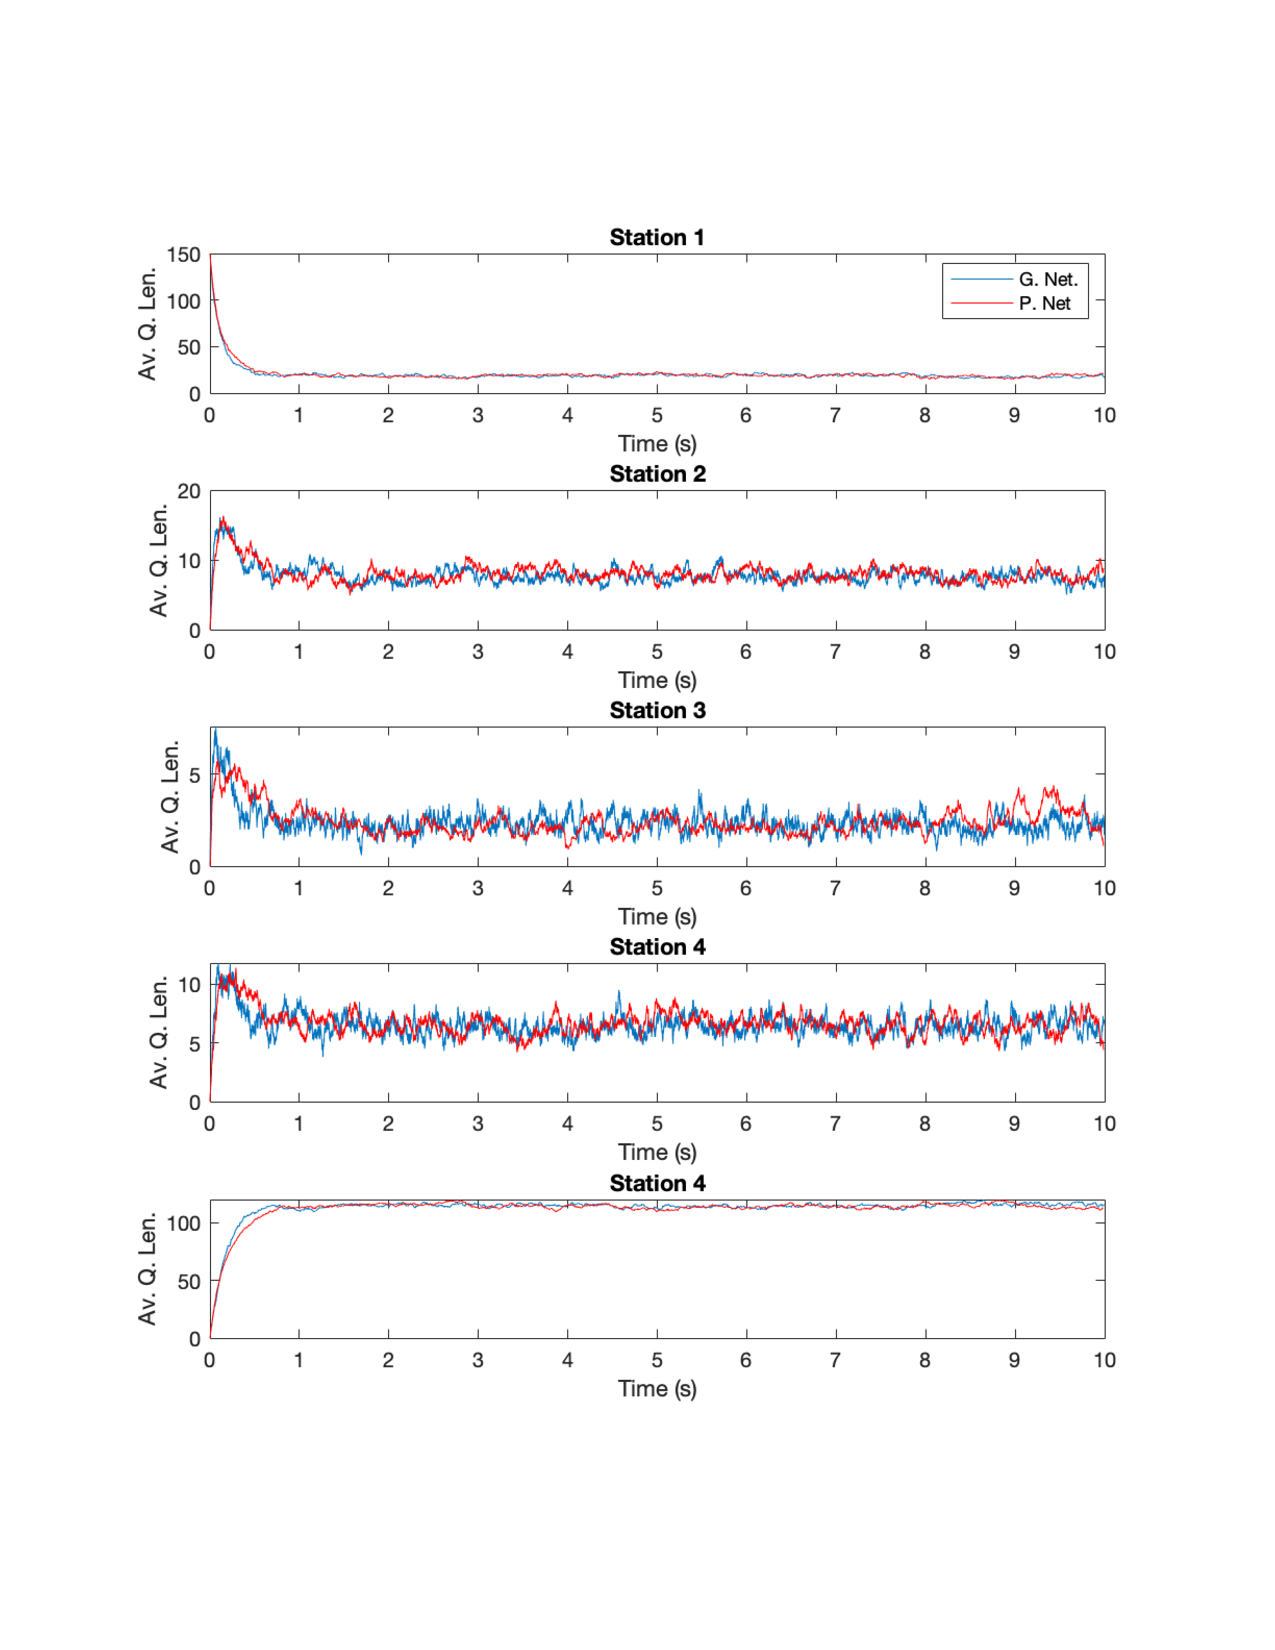
\includegraphics[width=120mm, scale=0.5]{av_q_len_5_stations.pdf}
\caption{Average Queue Length for 5 Stations}
\label{fig:av_q_length_5_stations}
\end{center}
\end{figure}

\textbf{Utilization}: Figure \ref{fig:utilization_5_stations} shows the evolution of the utilization at each server for both the generated and predicted networks. Again, we see that in the predicted network the utilization follows the same pattern as that of the generated network for every station. Therefore, our model predicts this metric well. \\

\textbf{Error Value and Absolute Difference in Average Queue Length}: The error in our model prediction is 7\%. Figure \ref{fig:abs_diff_5_stations} shows the absolute difference in average queue length for the generated and predicted network for each station. We can see that on average: 2 jobs are misplaced at station 1; 1 job is misplaced at station 2; 0.5 jobs are misplaced at station 3; 1 job is misplaced at station 4; and 2.5 jobs are misplaced at station 5. This is very good accuracy considering that there are 150 jobs in total in the system at any time. 

\begin{figure}[h!]
\begin{center}
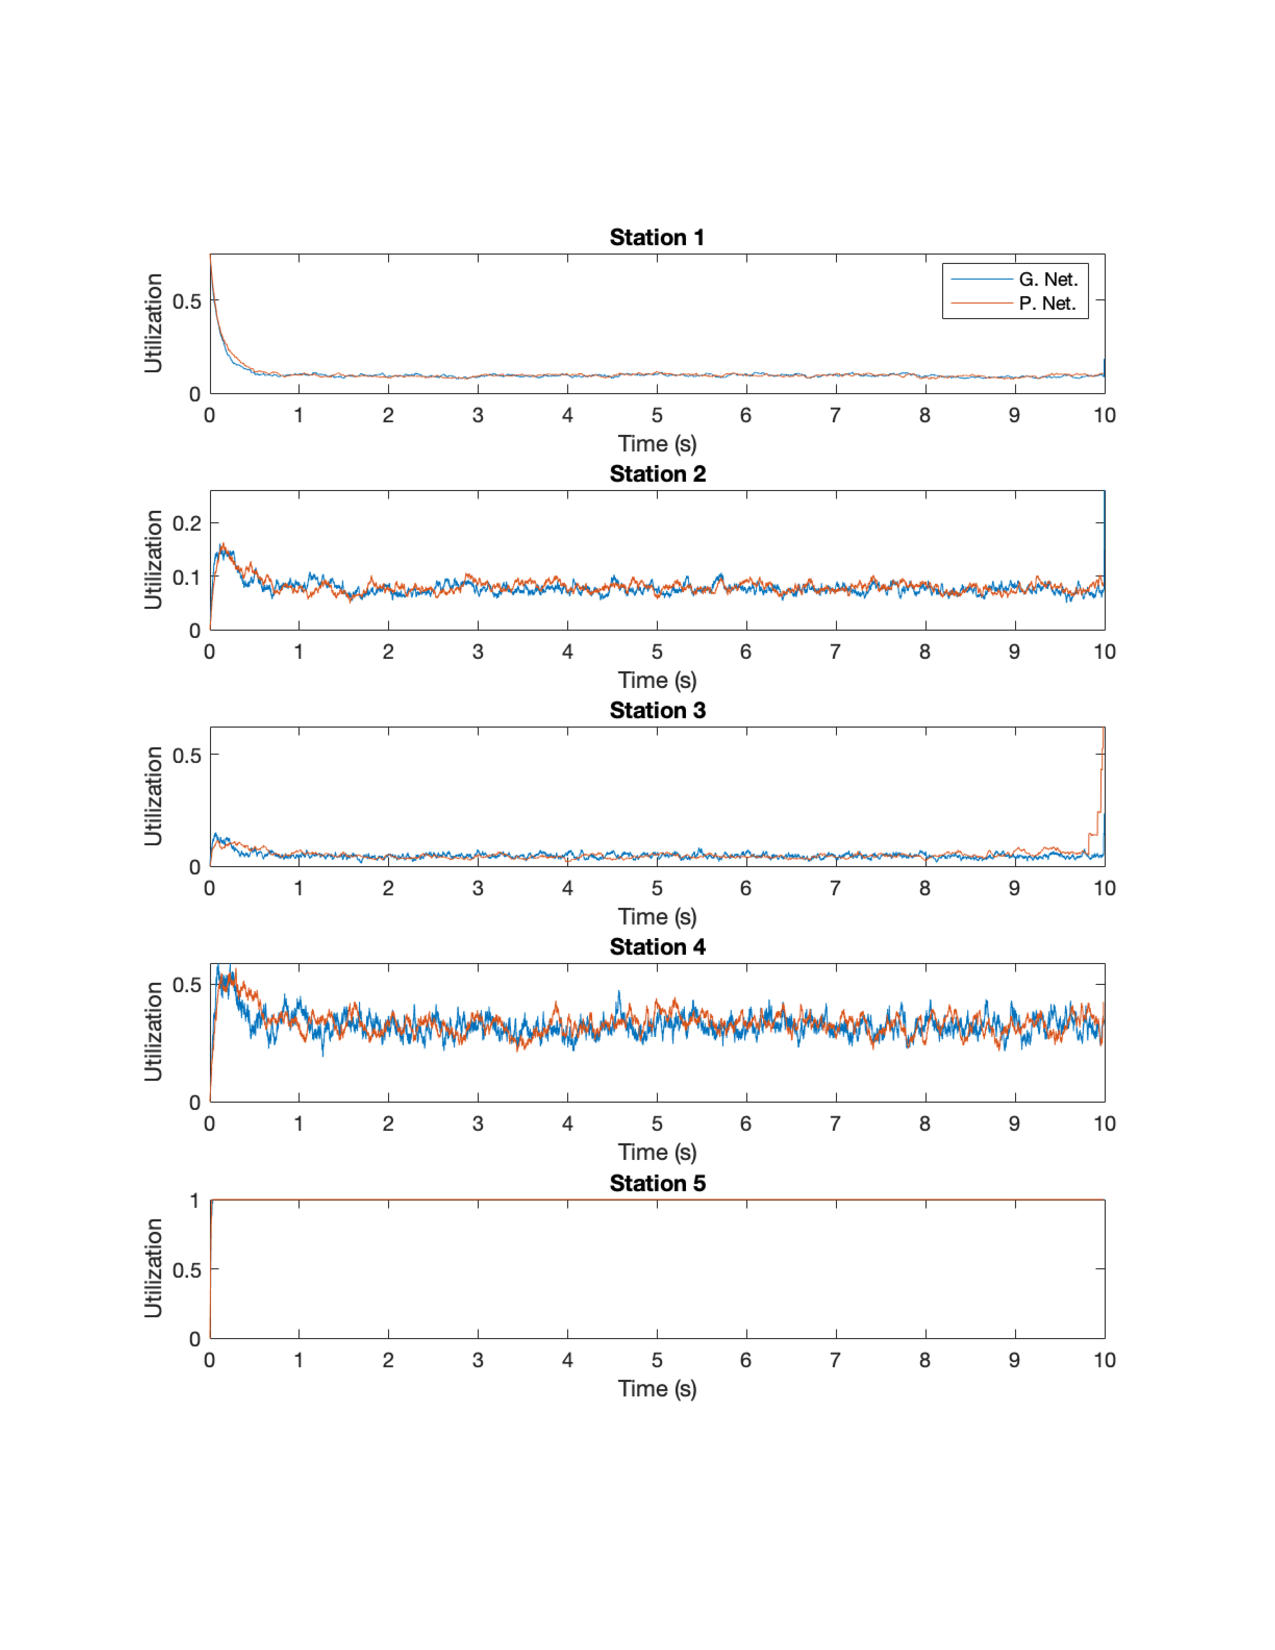
\includegraphics[width=120mm, scale=0.5]{utilization_5_stations.pdf}
\caption{Utilization for 5 Stations}
\label{fig:utilization_5_stations}
\end{center}
\end{figure}

\begin{figure}[h!]
\begin{center}
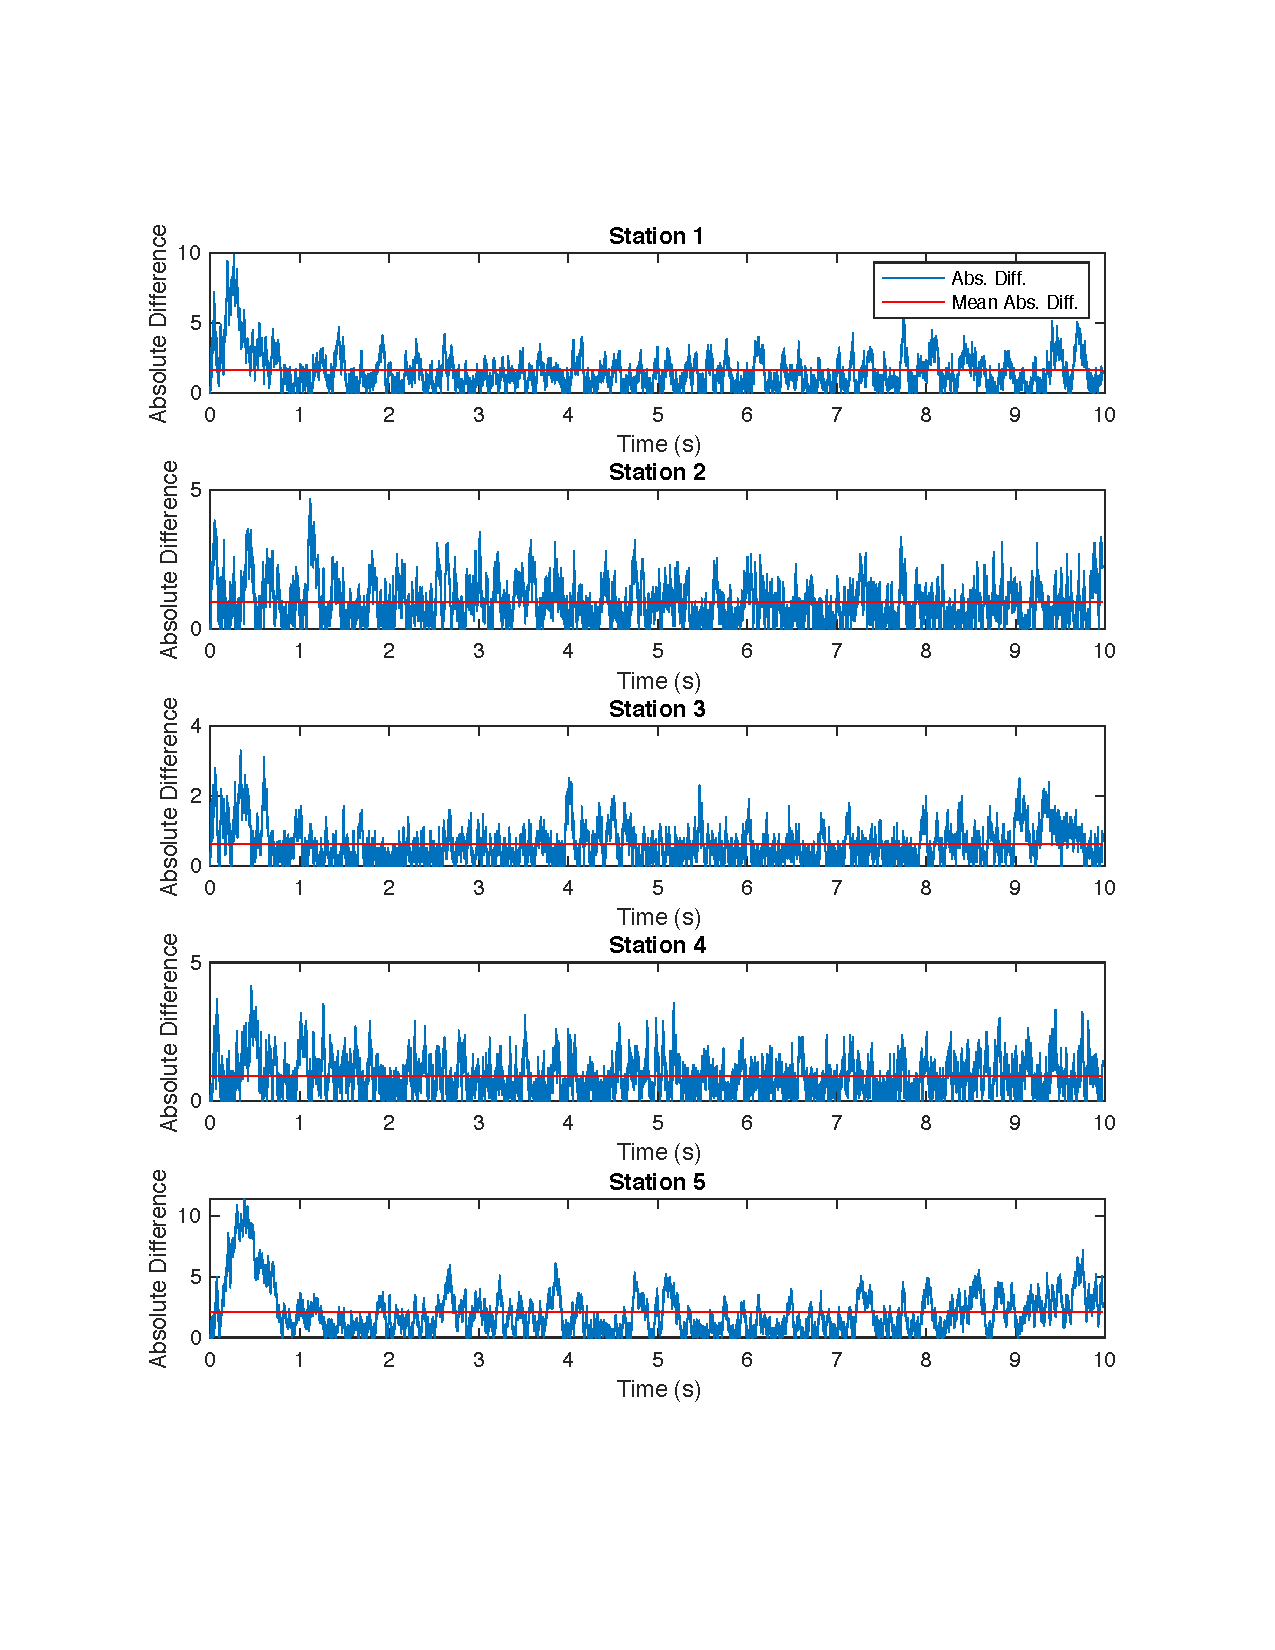
\includegraphics[width=120mm, scale=0.5]{abs_diff_5_stations.pdf}
\caption{Absolute Difference in Average Queue Length for 5 Stations}
\label{fig:abs_diff_5_stations}
\end{center}
\end{figure}

\subsection{Queueing Network with 10 Stations}: In this synthetic example we create traces using a queueing network with 10 stations, where $M=10$. For training our model, we set the server concurrency values to: $\mathbf{s} = [80,20,30,20,40,20,50,20,80,30]$; the service rates as $\bm{\mu} = [200,100,50,100,200,500,$ $200,100,200,100]$; and the initial population is randomly generated for each station and trace. We set the transition probability matrix of the generating queueing network as follows:
        
$$\mathbf{P} = \begin{bmatrix}
0 & 0.1 & 0.1 & 0.1 & 0.3 & 0 & 0.1 & 0.1 & 0.1 & 0.1 \\
0.05 & 0 & 0.15 & 0.2 & 0.1 & 0.2 & 0.1 & 0 & 0.1 & 0.1 \\
0.1 & 0.1 & 0 & 0.1 & 0.2 & 0.1 & 0.1 & 0.1 & 0.1 & 0.1\\
0.2 & 0.1 & 0.2 & 0 & 0.1 & 0 & 0.1 & 0.1 & 0.1 & 0.1 \\
0.2 & 0.1 & 0.1 & 0.1 & 0 & 0.1 & 0.1 & 0.1 & 0.1 & 0.1 \\
0.1 & 0.1 & 0.2 & 0.1 & 0.1 & 0 & 0.1 & 0.1 & 0.1 & 0.1 \\
0.1 & 0.2 & 0.1 & 0.1 & 0.1 & 0.1 & 0 & 0.1 & 0.1 & 0.1 \\
0.1 & 0.1 & 0.1 & 0.1 & 0.1 & 0 & 0.1 & 0 & 0.3 & 0.1 \\
0.1 & 0.1 & 0.1 & 0.1 & 0.1 & 0.2 & 0.1 & 0.1 & 0 & 0.1 \\
0.1 & 0.1 & 0.1 & 0.1 & 0.1 & 0.2 & 0.1 & 0.1 & 0.1 & 0 
\end{bmatrix} $$

where each row in $\mathbf{P}$ sums to 1 due to the stochasticity of the matrix, and there are no self-loops in the system. We then put the traces of the average queue lengths of each station over time through our RNN algorithm, which gives us a predicted model. Subsequently, we evaluate our model by using server concurrency values of $\mathbf{s} = [70,10,40,10,20,40,20,30,60,20]$ and initial population values of $ \mathbf{x}_0 = [250,0,0,0,0,0,0,0,0,0]$. We can then see how the generated and predicted networks compare. \\

For this generated queueing network, we have that the predicted network has the following parameters: 

$$ \bm{\mu} = [184.81, 14.70, 16.87, 13.40, 55.37, 22.42, 22.17, 15.76, 17.81, 13.42]$$

$$\mathbf{P} = \begin{bmatrix}
0.0 & 0.13 & 0.13 & 0.12 & 0.19 & 0.023 & 0.070 & 0.13 & 0.076 & 0.12\\
0.85 & 0.0 & 0.025 & 0.008 & 0.077 & 0.003 & 0.004 & 0.019 & 0.004 & 0.006\\
0.70 & 0.028 & 0.0 & 0.002 & 0.18 & 0.001 & 0.051 & 0.013 & 0.009 & 0.007 \\
0.70 & 0.004 & 0.004 & 0.0 & 0.17 & 0 & 0.073 & 0.039 & 0.005 & 0.003 \\
0.31 & 0.021 & 0.50 & 0.12 & 0.0 & 0.017 & 0.001 & 0.025 & 0.002 & 0.012 \\
0.59 & 0.087 & 0.058 & 0.013 & 0.15 & 0.0 & 0.038 & 0.056 & 0.002 & 0.01 \\
0.89 & 0.011 & 0.017 & 0.014 & 0.029 & 0.015 & 0.0 & 0.013 & 0.002 & 0.008 \\
0.84 & 0.009 & 0.057 & 0.012 & 0.057 & 0.011 & 0.005 & 0.0 & 0.004 & 0.005\\
0.85 & 0.017 & 0.032 & 0.017 & 0.031 & 0.038 & 0.001 & 0.01 & 0.0 & 0.005 \\
0.65 & 0.07 & 0.02 & 0.007 & 0.18 & 0.01 & 0.003 & 0.055 & 0.002 & 0.0
\end{bmatrix} $$ \\

where we have rounded the values in both the service rates and the transition probability matrix to 2 decimal places after the first non-zero decimal place. \\

We will now explore the performance metrics of the generated and predicted queueing networks and see how they compare. We will consider the metrics: average queue length, utilization, accuracy and absolute difference in average queue length. We will not consider the metric throughput as this is determined by the service rates, which is not a suitable consideration for the quality of our predictions. \\

As expected, when running our RNN model on a queueing network with 10 stations this took far longer than both the 3-station and 5-station algorithms. It took 4 times as long to run this algorithm, most likely due to the fact that the queueing network is much more complex: it has a higher initial number of jobs in the system; a higher vector of server concurrency values; and obviously a larger amount of stations. Additionally, it took a much longer amount of time to generate the 100 traces of the average queueing lengths. \\

\textbf{Average Queue Length at Each Station}: Figure \ref{fig:av_q_len_10_stations} shows the evolution in the average queue length at each station for both the predicted and generated networks. The predicted network is shown by the red line and the generated network is shown by the blue line. We can see that for most stations there is an accurate prediction of the average queue length, however at station 2 and station 4 there is a large discrepancy. We have that the average queue length for both networks converge to a similar value, however the pattern in the evolution is very different. Our model must have struggled to predict the parameters of the network for these 2 stations: perhaps because the network is slightly too complicated to get very accurate results; or perhaps our chosen example has some interesting complexities that other 10-station queueing networks would not have. \\ 

\begin{figure}[h!]
\begin{center}
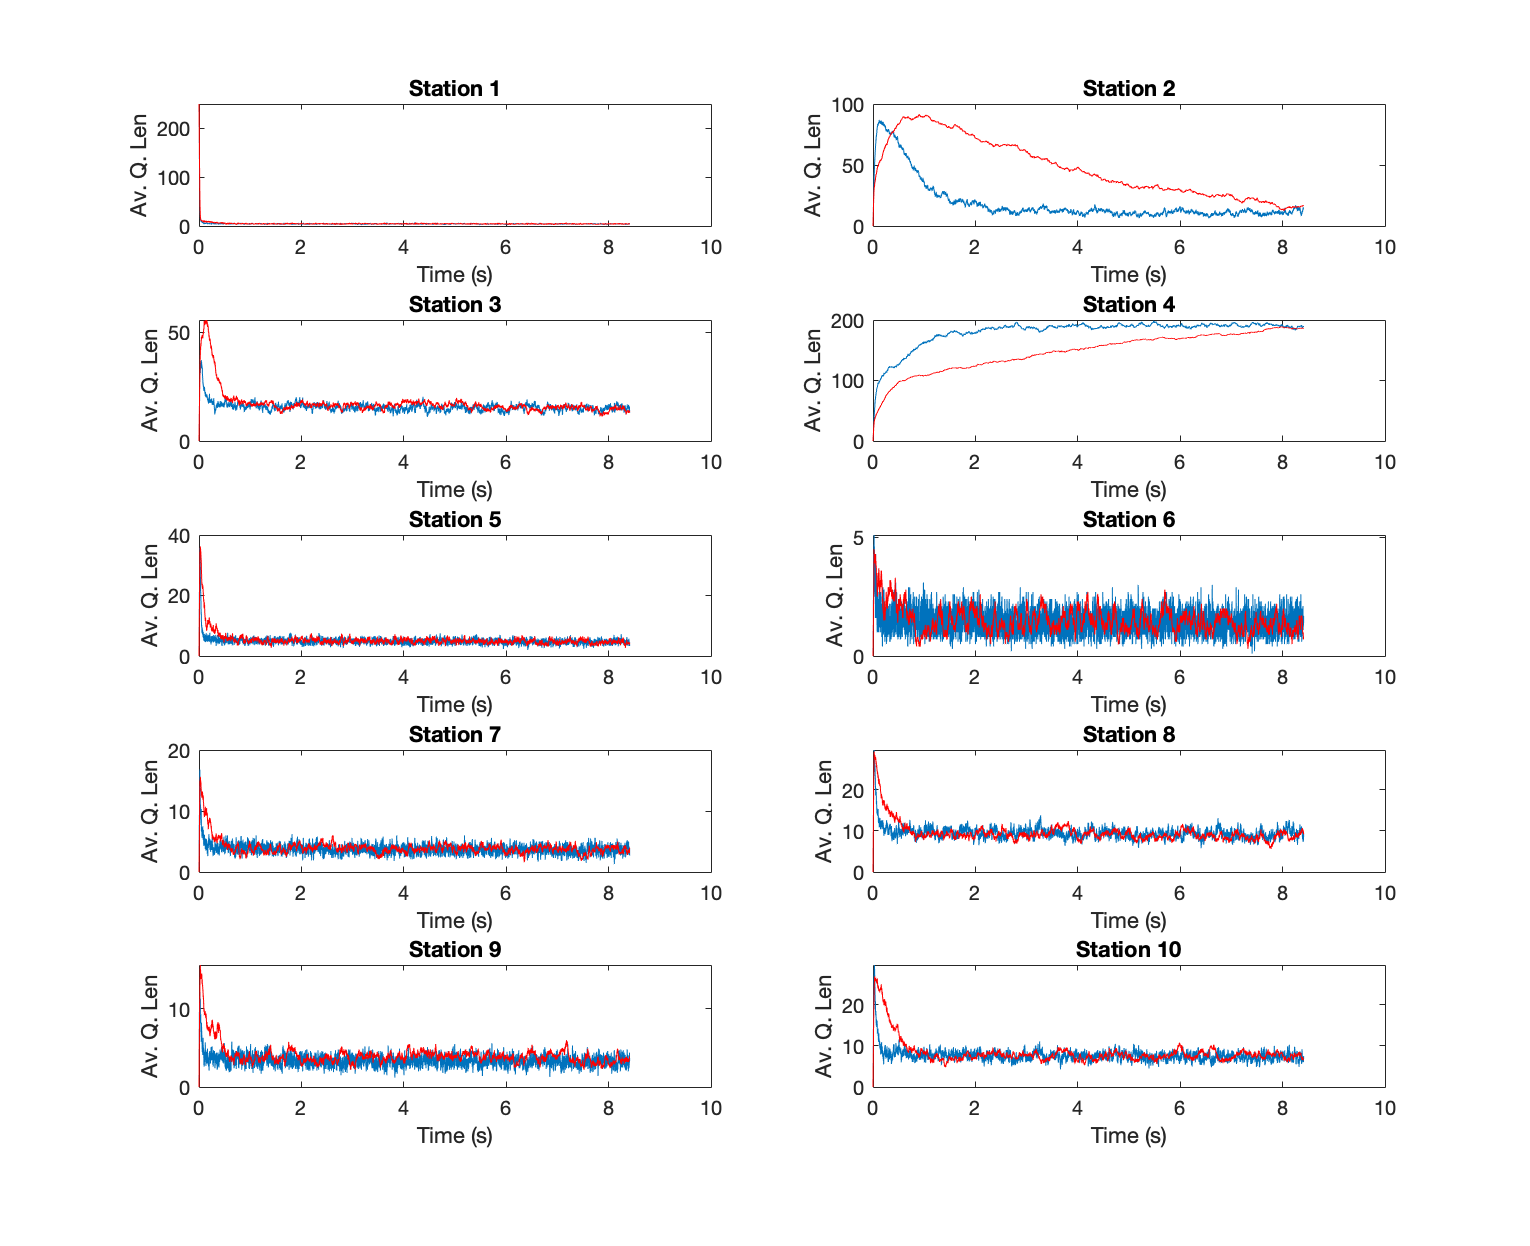
\includegraphics[width=\linewidth, scale=0.5]{av_q_len_10_stations.png}
\caption{Average Queue Length for 10 Stations}
\label{fig:av_q_len_10_stations}
\end{center}
\end{figure}

\textbf{Utilization at Each Station}: Figure \ref{fig:utilization_10_stations} shows the utilization for the generated and predicted networks at each station. The blue line denotes the evolution of the utilization for the generated network, and the red line the predicted network. We have that the utilization for each station is predicted with a high accuracy. \\

\begin{figure}[h!]
\begin{center}
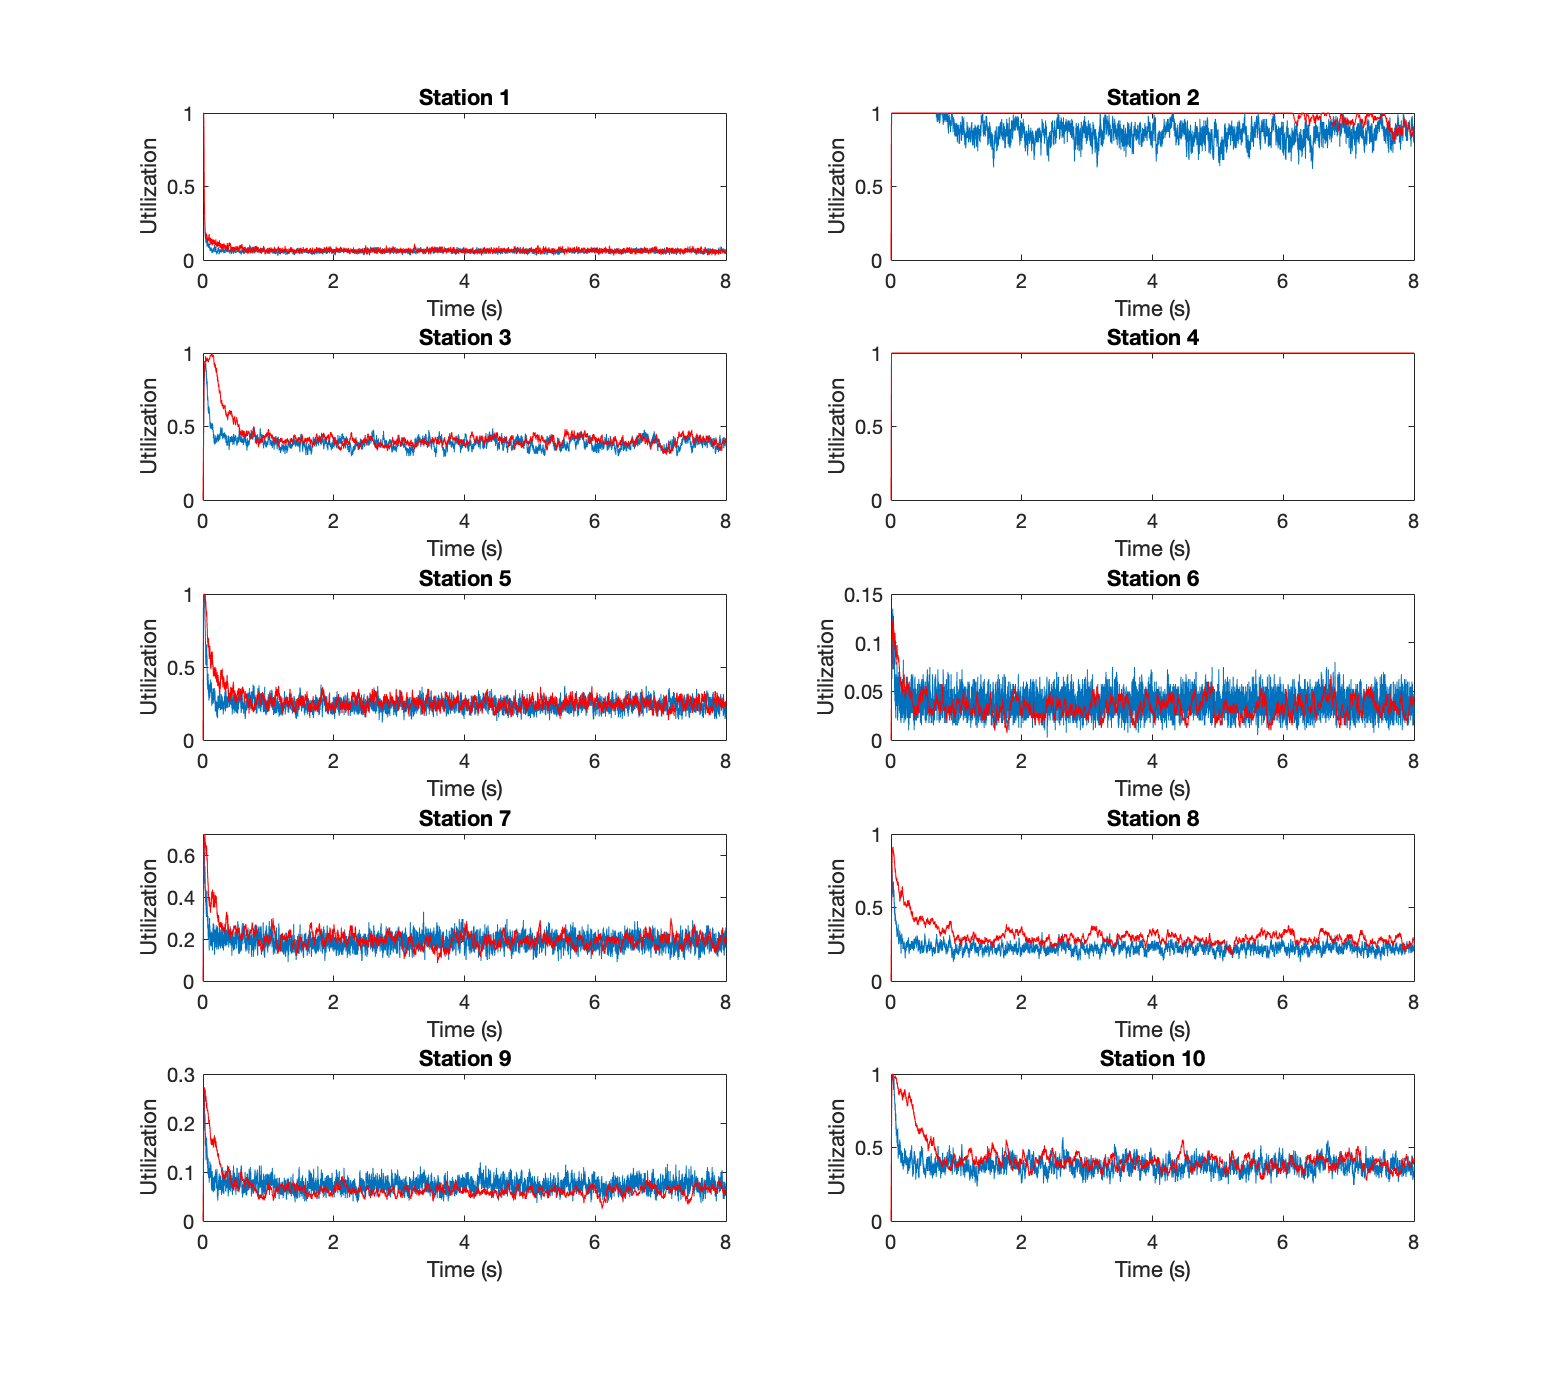
\includegraphics[width=\linewidth, scale=0.5]{utilization_10_stations.png}
\caption{Utilization for 10 Stations}
\label{fig:utilization_10_stations}
\end{center}
\end{figure}

\textbf{Error and Absolute Difference in Average Queue Lengths}: In the 10-station case, we have a higher error in our prediction compared to the other 2 examples. We have that this model has a 29\% error. This could be due to the fact that the queueing network is much more complex with a much higher number of weights and parameters to predict. The blue line denotes the evolution of the average queue length for the generated network, and the red line the predicted network. As we can see from the Figure \ref{fig:abs_diff_10_stations} the evolution is predicted accurately for most stations. We have some discrepancy in our prediction of the evolution in station 2 and station 4, where even though the average queue length eventually reaches a similar value, the pattern of the evolution is different. This is an interesting situation, where we can conclude that when our queueing network is more complex, our model struggles to accurately predict the average queue length with a high accuracy for every station: something in the predicted parameters of the network is not quite right. We have on average: 2 jobs misplaced at station 1; 35 jobs misplaced at station 2; 3 jobs misplaced at station 3; 40 jobs misplaced at station 4; 2 jobs misplaced at station 5; 1 job misplaced at station 6; 1 job misplaced at station 7; 1.5 jobs misplaced at station 8; 1 job misplaced at station 9; and 2 jobs misplaced at station 10. If we redo the experiment with a different probability transition matrix and service rate vector for another generating network, we may get better results.

\begin{figure}[h!]
\begin{center}
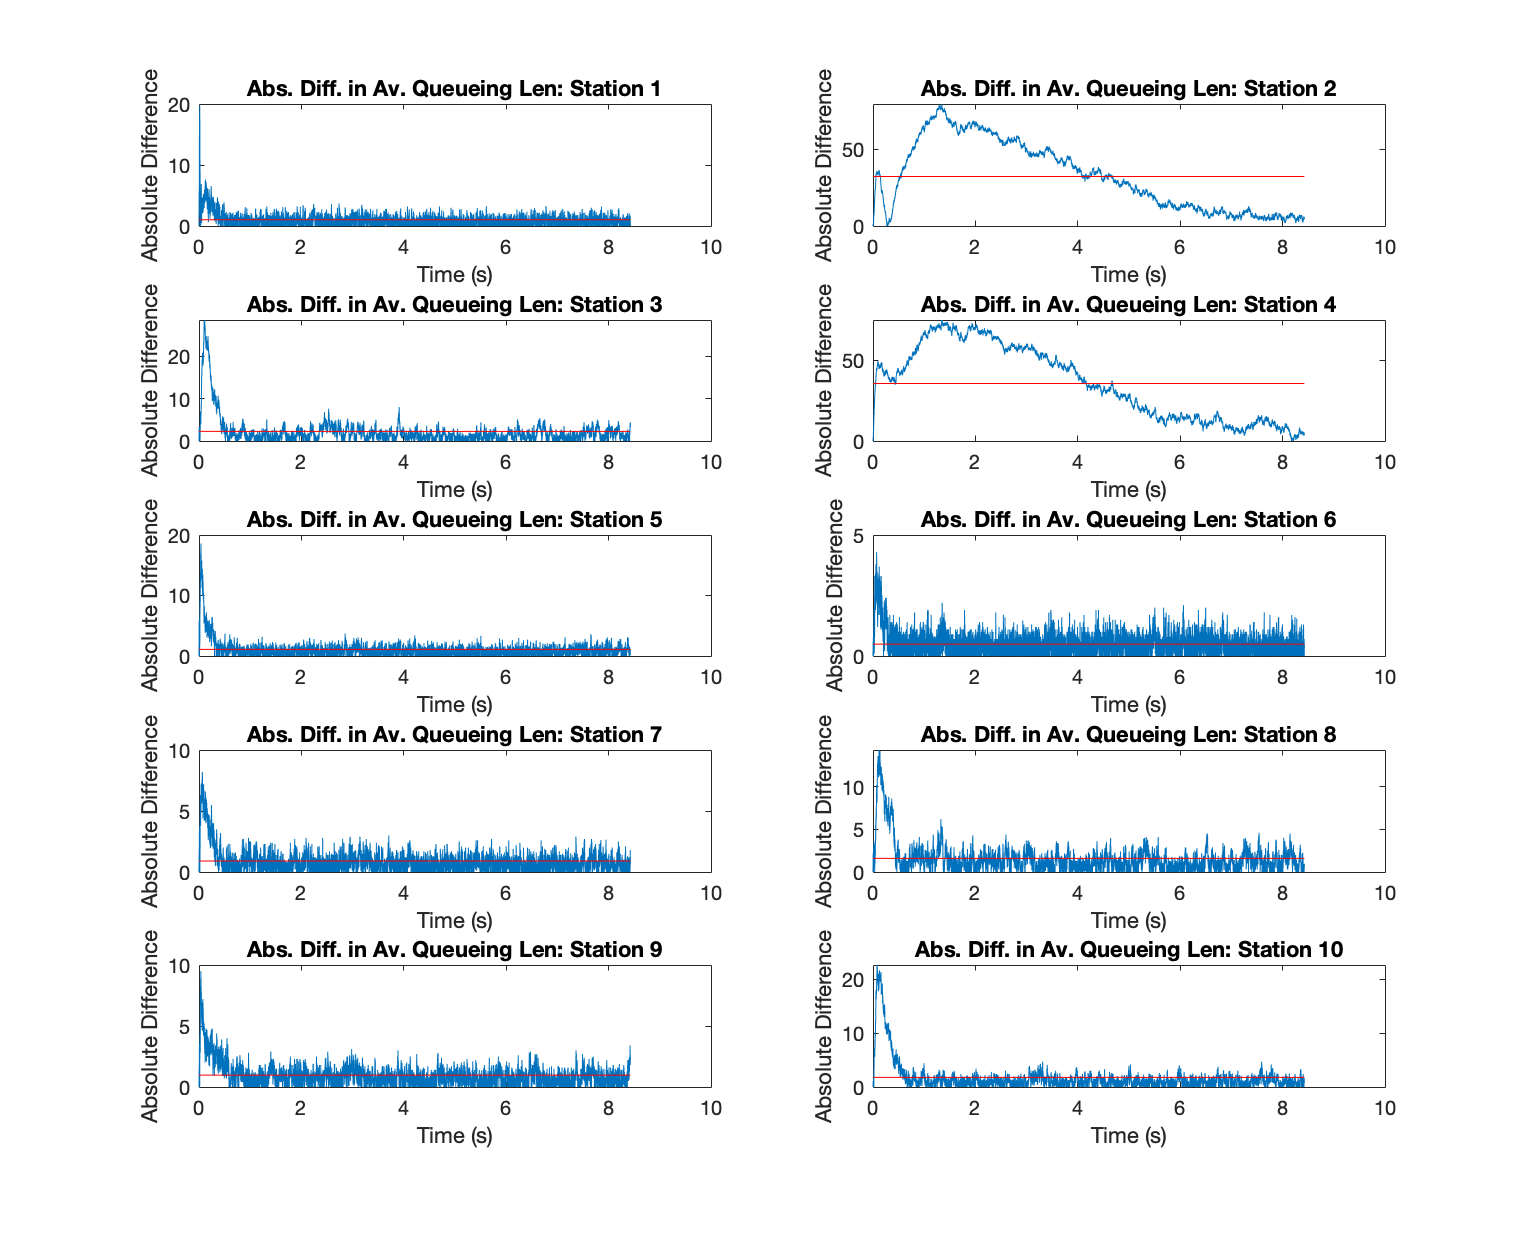
\includegraphics[width=\linewidth, scale=0.5]{abs_diff_10_stations.png}
\caption{Absolute Difference in Average Queue Length for 10 Stations}
\label{fig:abs_diff_10_stations}
\end{center}
\end{figure}

\subsection{Conclusions Regarding the RNN Model on our Example Queueing Networks}

\begin{figure}[h!]
\begin{center}
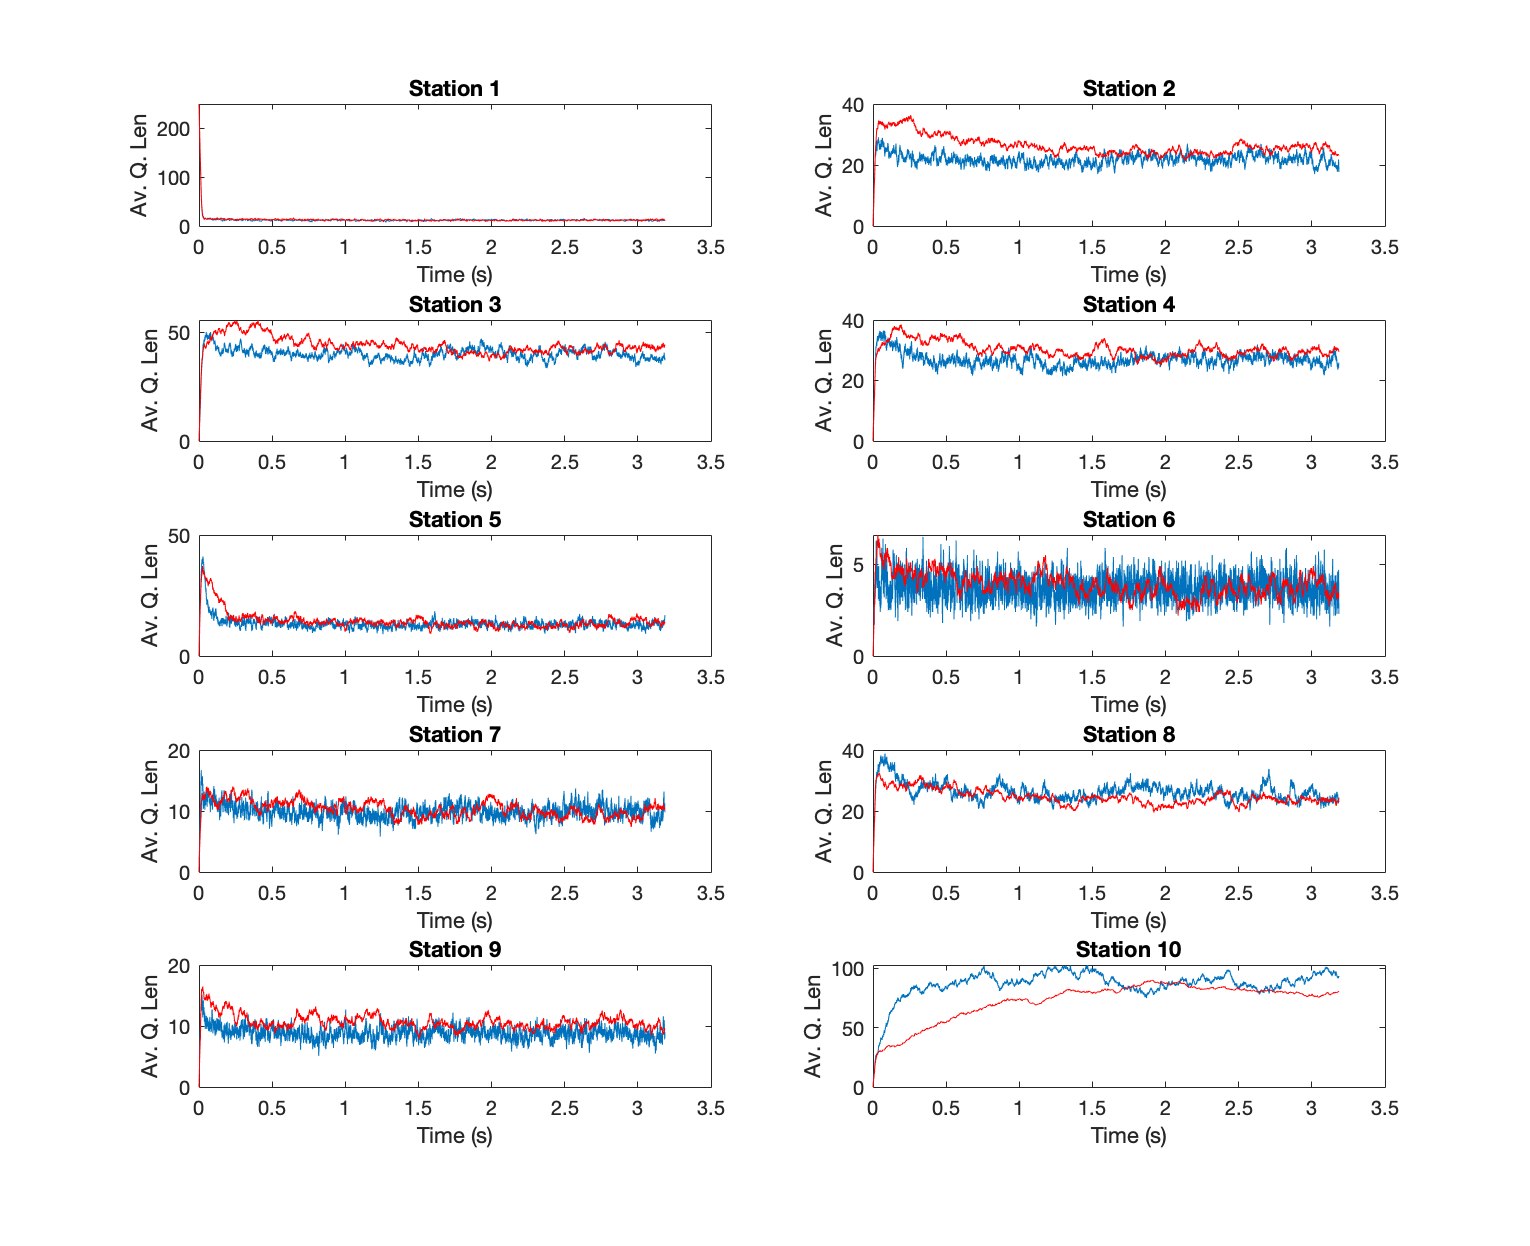
\includegraphics[width=\linewidth, scale=0.5]{av_q_len_concurrency_changed.png}
\caption{Average Queue Length with Changed Concurrency Values}
\label{fig:av_q_len_server_increased}
\end{center}
\end{figure}

We have analysed examples of our model working very well for both 3-station and 5-station queueing networks. Our RNN model works well on these examples because the error in both is very low, and we have shown that the prediction of certain metrics are of high quality. Our RNN model predicts the fluid approximations of the dynamics of the networks very well for each station, and hence provides predictions for the parameters of the queueing networks with a high degree of accuracy to give predictions that match the behaviour very well of the generating network. \\

The more interesting scenario is that of the queueing network with 10 stations. We can ask ourselves the question: what went wrong in the RNN model to give us a prediction error of 29\%, when the 3-station scenario had an error of 4.96\% and the 5-station scenario had an error of 7\% respectively? One explanation could be that because the amount of parameters that we need to accurately estimate grows exponentially with regard to the station size, queueing networks with more stations will be more complicated to predict accurately. This is due to the following explanation: to predict the topology of the 3-station network we only needed to estimate the 6 transition probabilities and the 3 service rates in $\bm{\mu}$. In the 5 station example we needed to predict 20 transition probabilities and 5 service rates. For the 10-station example we needed to predict 90 transition probabilities and 10 service rates. Therefore, for a queueing network with $M$ stations, our algorithm is required to predict $M(M-1)$ transition probabilities and $M$ service rates (note that the diagonal of the matrix is constrained to 0). Furthermore, it is not just the increase in size of predictions that could cause a higher error. We will now discuss certain situations that may have occurred in our queueing network that could have created the inferior prediction for that example. \\

A situation that could have produced the inferior results is if were to have a severe bottleneck in one or more of the queueing stations in our network. A bottleneck is when we have a station that has a very high ratio between the steady state average queue length and the number of servers in that station. If we were to get a severe bottleneck scenario in either our generating network or our predicting network, then that may decrease the accuracy of our model. We had in our example that both the second station and the fourth station in our network only had 10 servers coupled with a high amount of traffic. Therefore, we had a high chance of bottlenecks occurring. It seems that we did have a bottleneck occur in these stations, as in Figure \ref{fig:av_q_len_10_stations} we can see that in station 4 the average queue length becomes very high the further along the evolution we go. It is interesting to note that we over-predict the average queue length in station 2, and under-predict the average queue length in station 4. It almost seems as if most of the jobs that we misplace in one of those stations should be in the other station. Therefore, in both of these stations, our model struggled to predict the correct evolution of the average queue length. Figure \ref{fig:av_q_len_server_increased} shows the average queue lengths of our generated and predicted models for all stations if we increase the server concurrency values in station 2 and station 4 to 60 from their original value of 10. \\

As we can see from the graph, the error of the average queue length in station 2 and station 4 has decreased when we increase the concurrency values in these two stations. We do have that the error has increased in station 10, although overall the error of the whole model prediction has decreased from 29\% to 19\%, which is a significant improvement. Therefore, when we create RNN algorithms for more complex queueing networks we need to consider how changing the server concurrency values factor affect our predictions. Figure \ref{fig:abs_diff_concurrency} shows the decrease in error of our model as less jobs are misplaced. There are other ways that we could have decreased the error of our model. When we evaluate the error of our model on a certain queueing network, we only take one run through to generate the average queue length in each station for both the predicted and generated queueing networks. If we were to take an average of say 100 evolutions of the average queue length at each station for both networks then we would limit any anomalous results which may give us a better and more accurate error value. \\

Overall, our RNN-model has shown to be able to accurately predict the parameters and behaviour of a few quite simple examples of queueing networks. Therefore, we can conclude that the RNN-methodology is a suitable machine learning technique to use to predict parameters of queueing networks. It does seem that the error in our predictions are quite dependent on the server concurrency values that we choose for learning and prediction. There are many examples of unseen concurrency values that give great results; however there are also some examples of server concurrency values that give inferior results. The reference [Gar20] covers this in more detail, as they do a similar experimentation over what-if analyses using many more examples than we have here. They predict the error of their models on hundreds of different queueing networks initialized with different server concurrency values and initial populations and achieve very accurate results. \\

Table \ref{tab:eval_rnn} shows the error in average queue length prediction in our evaluation of the RNN methodology for predicting the topology of queueing networks for each of our example queueing networks. We also show the time complexity for generating the traces in LINE for each queueing network, and the time complexity for creating the model that is used for prediction, where each time is rounded to the nearest hour. In the left-hand column, `M' denotes the number of stations, `10.1' denotes the first attempt with 10 stations, and `10.2' denotes the second attempt with 10 stations. 

\begin{table}[]
\begin{tabular}{|c|c|c|c|}
\hline
M & \multicolumn{1}{l|}{Error In Prediction} & \multicolumn{1}{l|}{Time for Trace Generation} & \multicolumn{1}{l|}{Time for Model Prediction} \\ \hline
3 & 5.4\% & 2 hours & 3 hours \\ \hline
5 & 7\% & 5 hours & 7 hours \\ \hline
10.1 & 29\% & 12 hours & 18 hours \\ \hline
\multicolumn{1}{|l|}{10.2} & 19\% & 12 hours & 18 hours \\ \hline
\end{tabular}
\caption{Performance Metrics for RNN methodology Evaluation on Example Queueing Networks}
\label{tab:eval_rnn}
\end{table}

\begin{figure}[h!]
\begin{center}
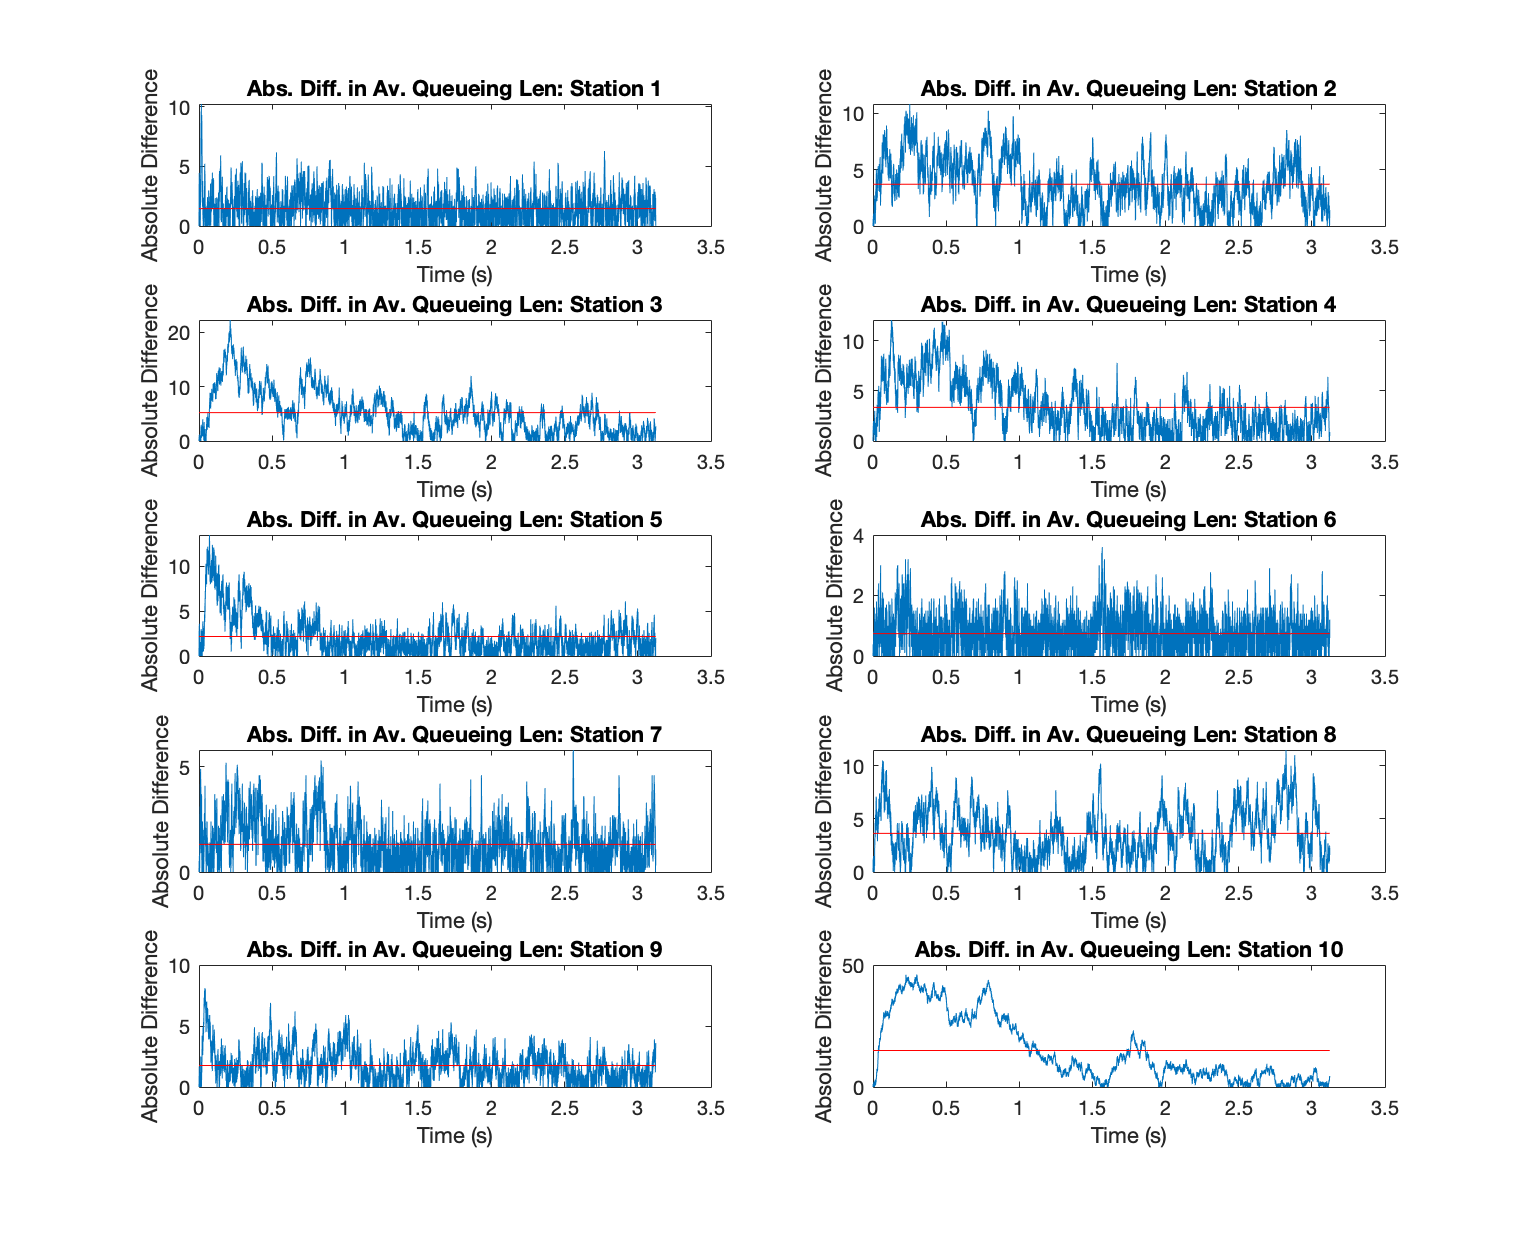
\includegraphics[width=\linewidth, scale=0.5]{abs_diff_server_increased.png}
\caption{Absolute Difference in Average Queue Lengths with Changed Server Concurrency Values}
\label{fig:abs_diff_concurrency}
\end{center}
\end{figure}

\subsection{Sensitivity of Server Concurrency Values for our Model}

In this section we will analyse the sensitivity of our RNN model to changing server concurrency values. As explained previously, changing the server concurrency values can dramatically alter the behaviour of the queueing network. When we change these values, the bottlenecks in certain stations move to other stations. Bottlenecks almost always occur within queueing systems [Buz71], and are an important research area of study [Buz71], [Wan05], [Kik16].  We have a hypothesis detailed as follows: if we use our predicted parameters on a queueing network that contains a severe bottleneck, then our prediction has the potential to give inferior accuracy for our results. The explanation for this could be that if we were to train our model on a network that never experiences a severe bottleneck in one of its stations, due to the server concurrency values that we use for training the model, then our model would have a hard time predicting the correct parameters for a network that does experience a severe bottleneck when using unseen server concurrency values. \\

\begin{figure}[h!]
\begin{center}
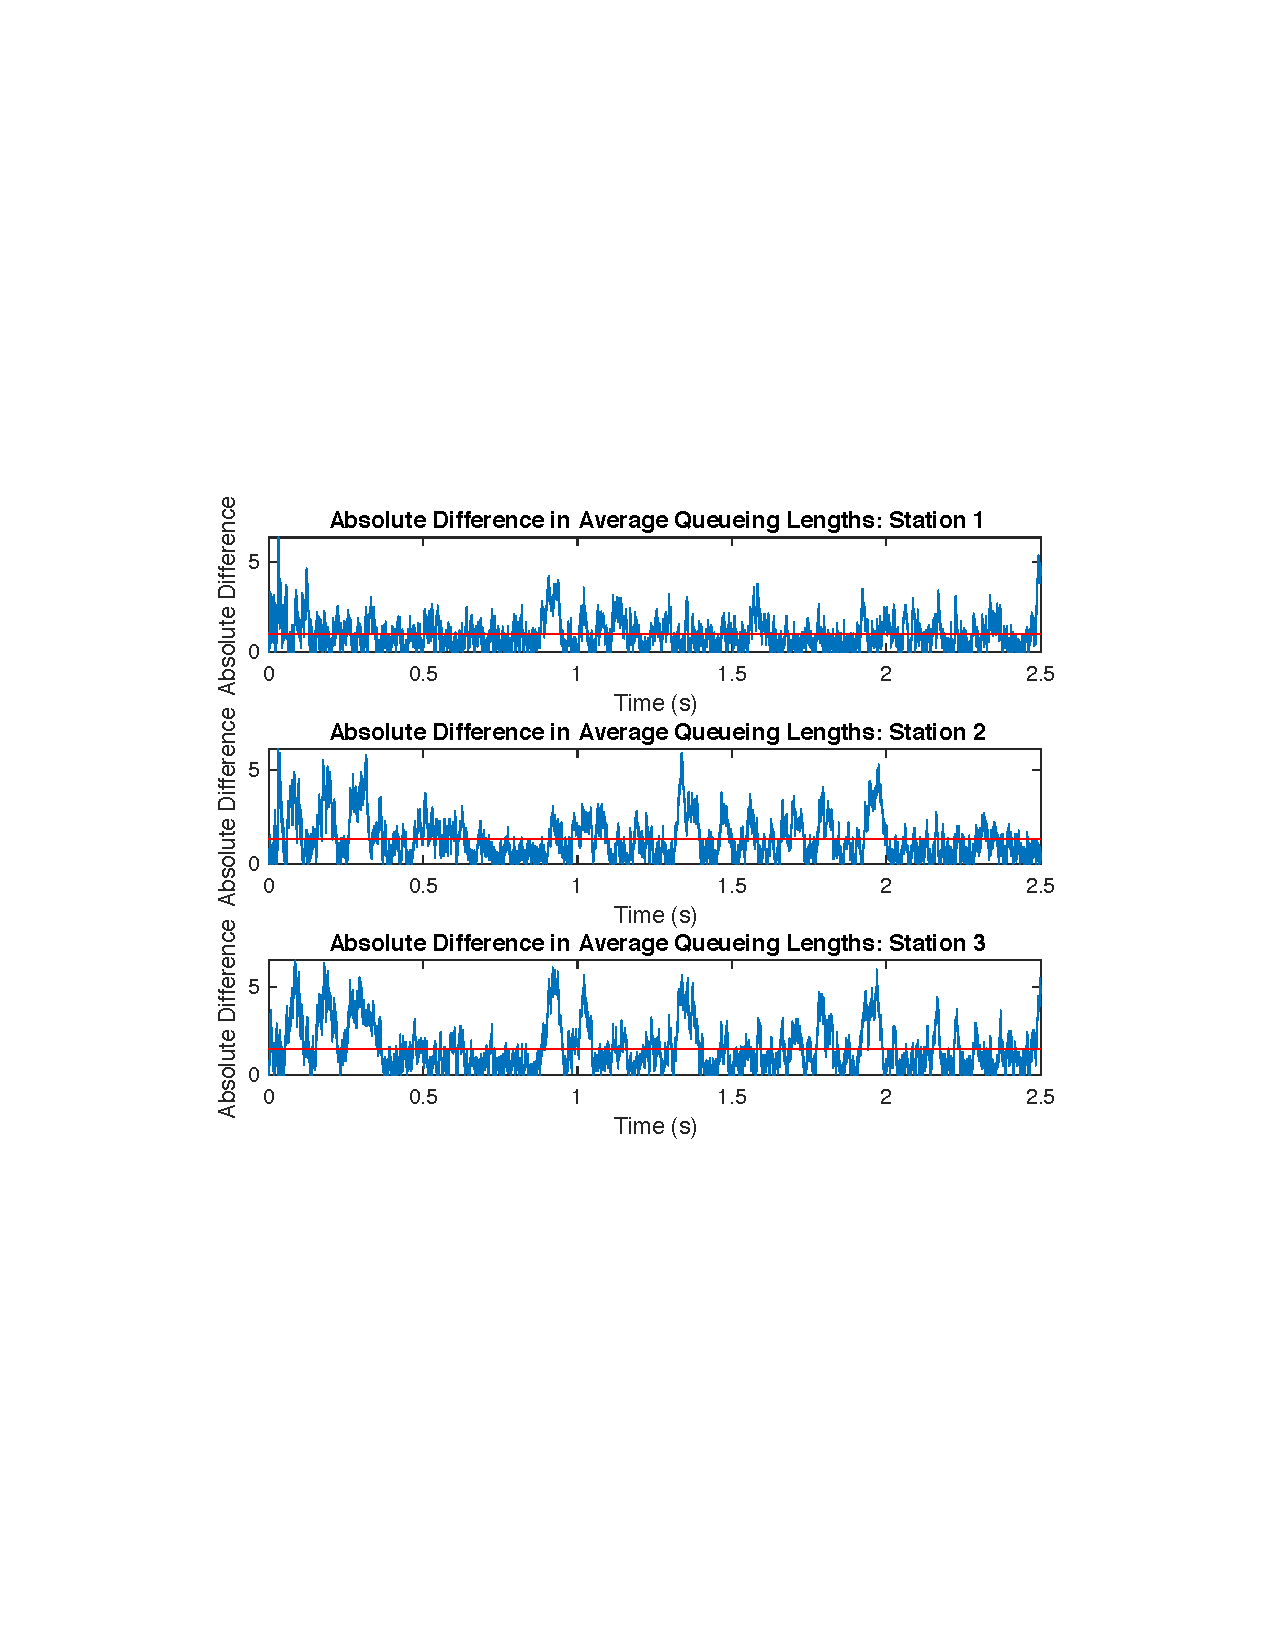
\includegraphics[width=120mm, scale=0.5]{bottleneck_reference_actual.pdf}
\caption{Absolute Difference in Average Queue Lengths without bottleneck: $err = 4.296\%$}
\label{fig:bottleneck_reference}
\end{center}
\end{figure}

To study how an intense bottleneck in one or more stations may affect our predictions we created a very simple experiment using a single class 3-station queueing network. We use the same network as the 3-station network from earlier in this chapter, where we set $\mathbf{s} = [40,20,10]$ as the server concurrency values for each station during the learning,  $\bm{\mu} = [100,50,50]$ as the service rates for each station, and a transition probability matrix of: 

\begin{equation}
    \mathbf{P} = \begin{bmatrix}
     0 & 2/3 & 1/3 \\
     1/3 & 0 & 2/3 \\
     2/3 & 1/3 & 0
    \end{bmatrix}.
\end{equation}

We already had the predicted model from our analysis of the 3-station RNN prediction in the previous section. We will now describe our experiment for evaluating how severe bottlenecks in stations affect the accuracy of our prediction. As a point of reference for accuracy, we analysed the error between the generated network and the RNN-learned network using 200 jobs in the network all starting in the 1st station and server concurrency values of $\mathbf{s} = [50,20,10]$. For this network, we found that our RNN-learned queueing network had a 4.2960\% error value. Therefore only 4.2960\% of jobs are misplaced at each time step on average. Figure \ref{fig:bottleneck_reference} shows the absolute difference in average queue length for the predicted and generated networks over a time period of 2.5s, where the red line denotes the mean absolute difference. Therefore, for this situation, our model predicts the parameters of the queueing network very well and gives a great prediction of the evolution of the average queue lengths. We will now show two examples of where we change the server concurrency values to synthetically create bottlenecks in the system. For these two examples we will show how changing the server concurrency values of the network alters the error of our prediction and the evolution of the average queue lengths in the generated and predicted networks. After looking at these 2 examples in detail we will explore how the error changes for other unseen server-concurrency values that we choose. \\

\begin{figure}[h!]
\begin{center}
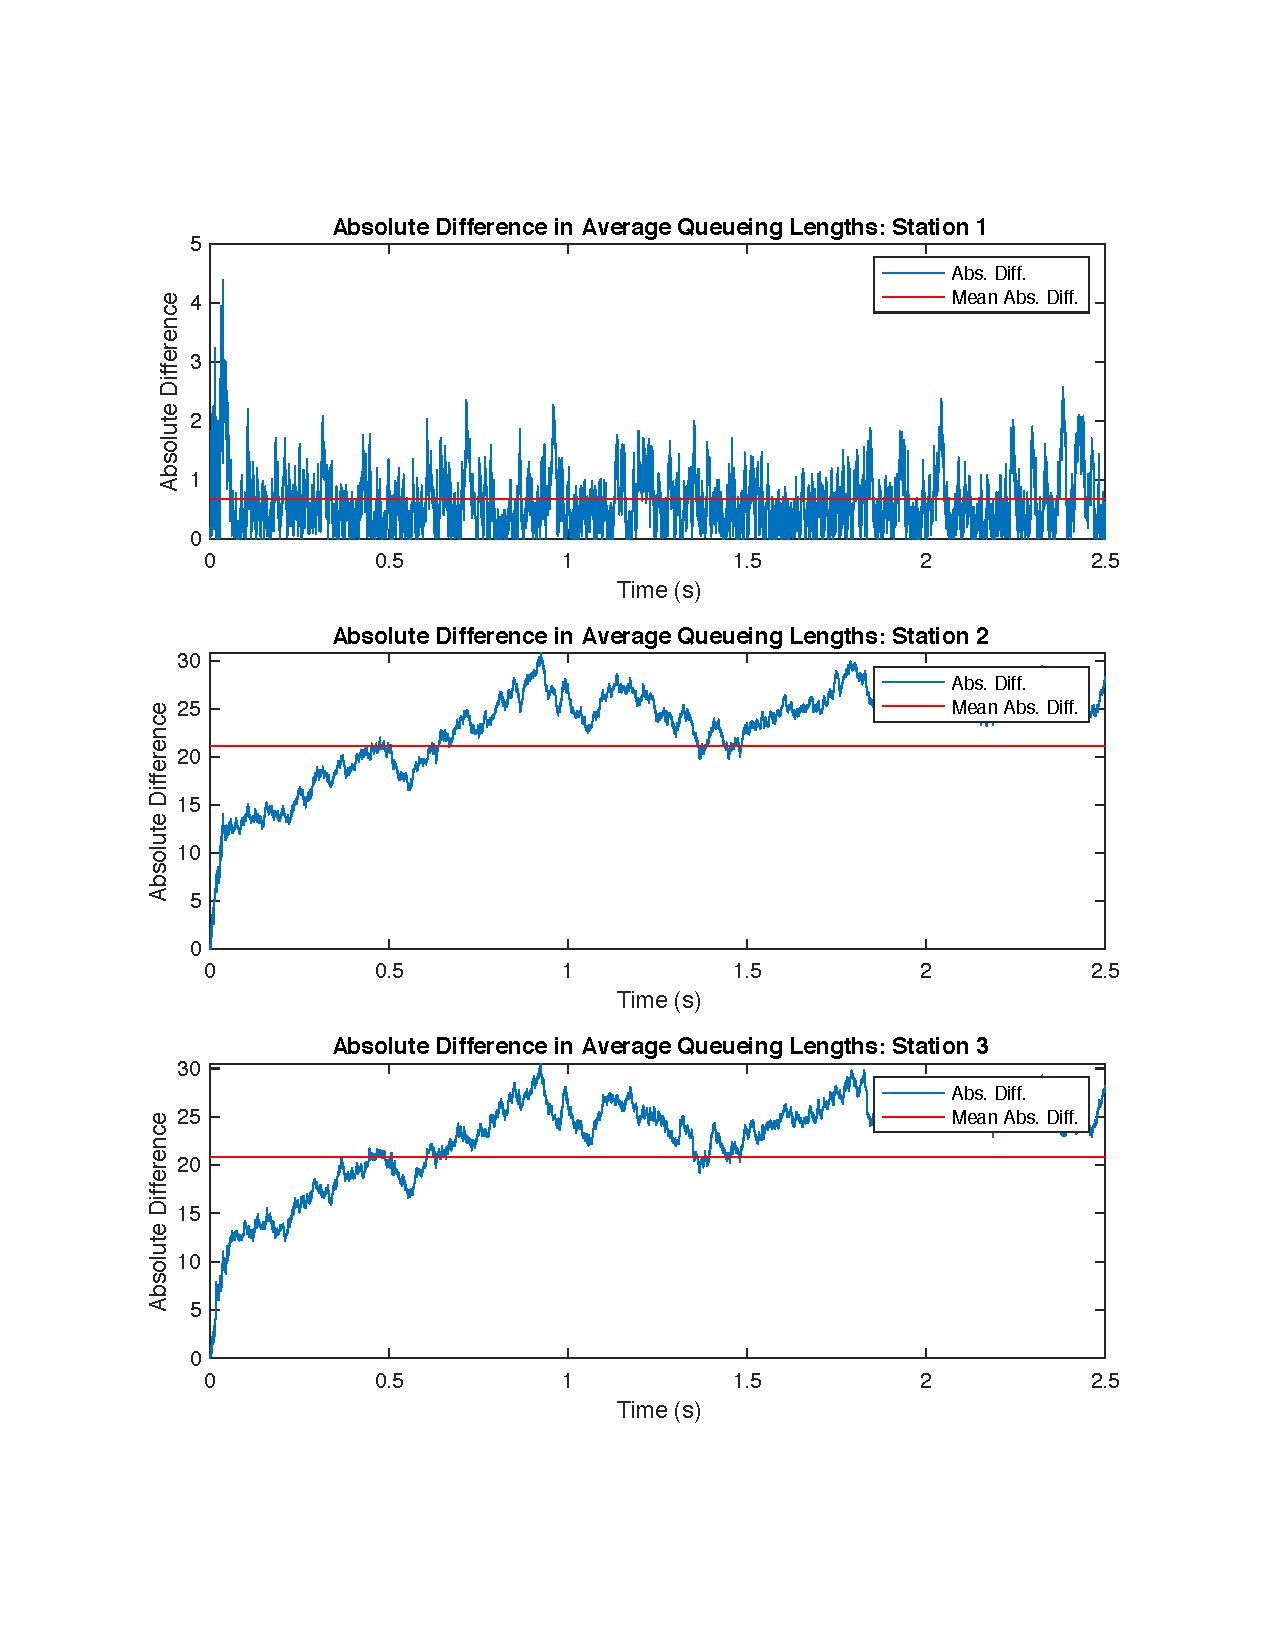
\includegraphics[width=100mm, scale=0.5]{abs_diff_bottleneck.pdf}
\caption{Absolute Difference in Average Queue Lengths with Bottleneck Ex. 1: $err = 15.7\%$}
\label{fig:bottleneck_ex_1}
\end{center}
\end{figure}

\textbf{Experiment 1 with Changed Server Concurrency Values}: For this experiment we will synthetically create severe bottlenecks in our system by decreasing the amount of servers in station 2 and station 3. As the ratio between the steady state average queue length and server concurrency values in these stations are high, we have created a synthetic bottleneck. We use the same population vector for the network. We change the server concurrency values to: $\mathbf{s} = [50,5,5]$. Our hypothesis is that when we create severe bottlenecks in our system the overall accuracy of our model decreases. As shown in Figure \ref{fig:bottleneck_ex_1}, the error of our model in this example has increased quite dramatically. We now have an error of 15.7\%. As seen in Figure \ref{fig:bottleneck_ex_1_q_len} the average queueing lengths are highly misrepresented in our predicted network for both station 2 and station 3. Therefore, this example agrees with the hypothesis that we have set. During learning, we had no bottleneck in the network, therefore our predicted model struggles to accurately predict the transient queue lengths when a bottleneck is introduced.  \\

\begin{figure}[h!]
\begin{center}
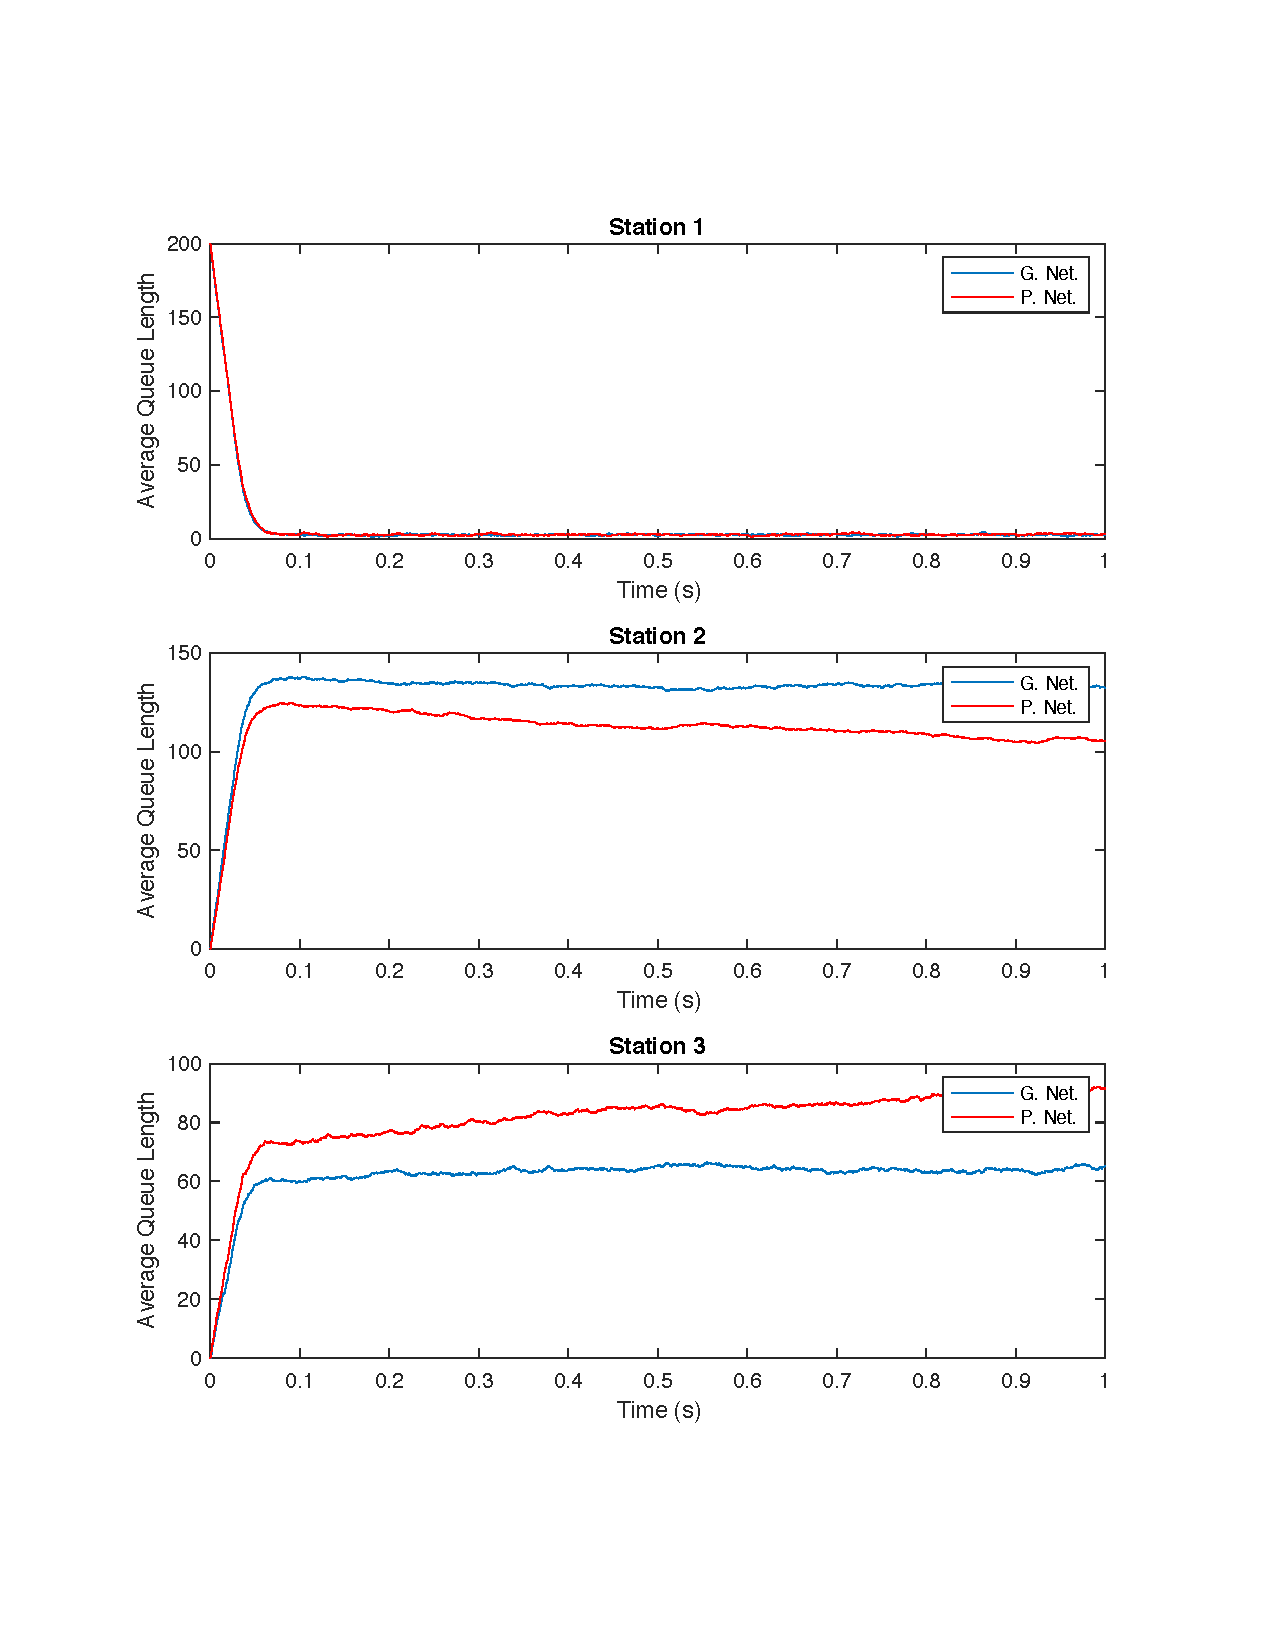
\includegraphics[width=100mm, scale=0.5]{av_q_len_bottleneck.pdf}
\caption{Average Queue Lengths with Bottleneck Ex. 1: $err = 15.7\%$}
\label{fig:bottleneck_ex_1_q_len}
\end{center}
\end{figure}

\textbf{Experiment 2 with Changed Server Concurrency Values}: For this experiment we keep 200 jobs in the network and we set the server concurrency values to $\mathbf{s} = [50,2,2]$. We assume the error in this prediction will once again be much larger than the reference error. Once performing the evaluation we found that we were correct, where the error in our prediction was a high $15.4\%$. Figure \ref{fig:bottleneck_ex_2} shows the absolute difference in average queue lengths, where we can see that in station 2 and station 3 we once again have a large misrepresentation. \\

\begin{figure}[h!]
\begin{center}
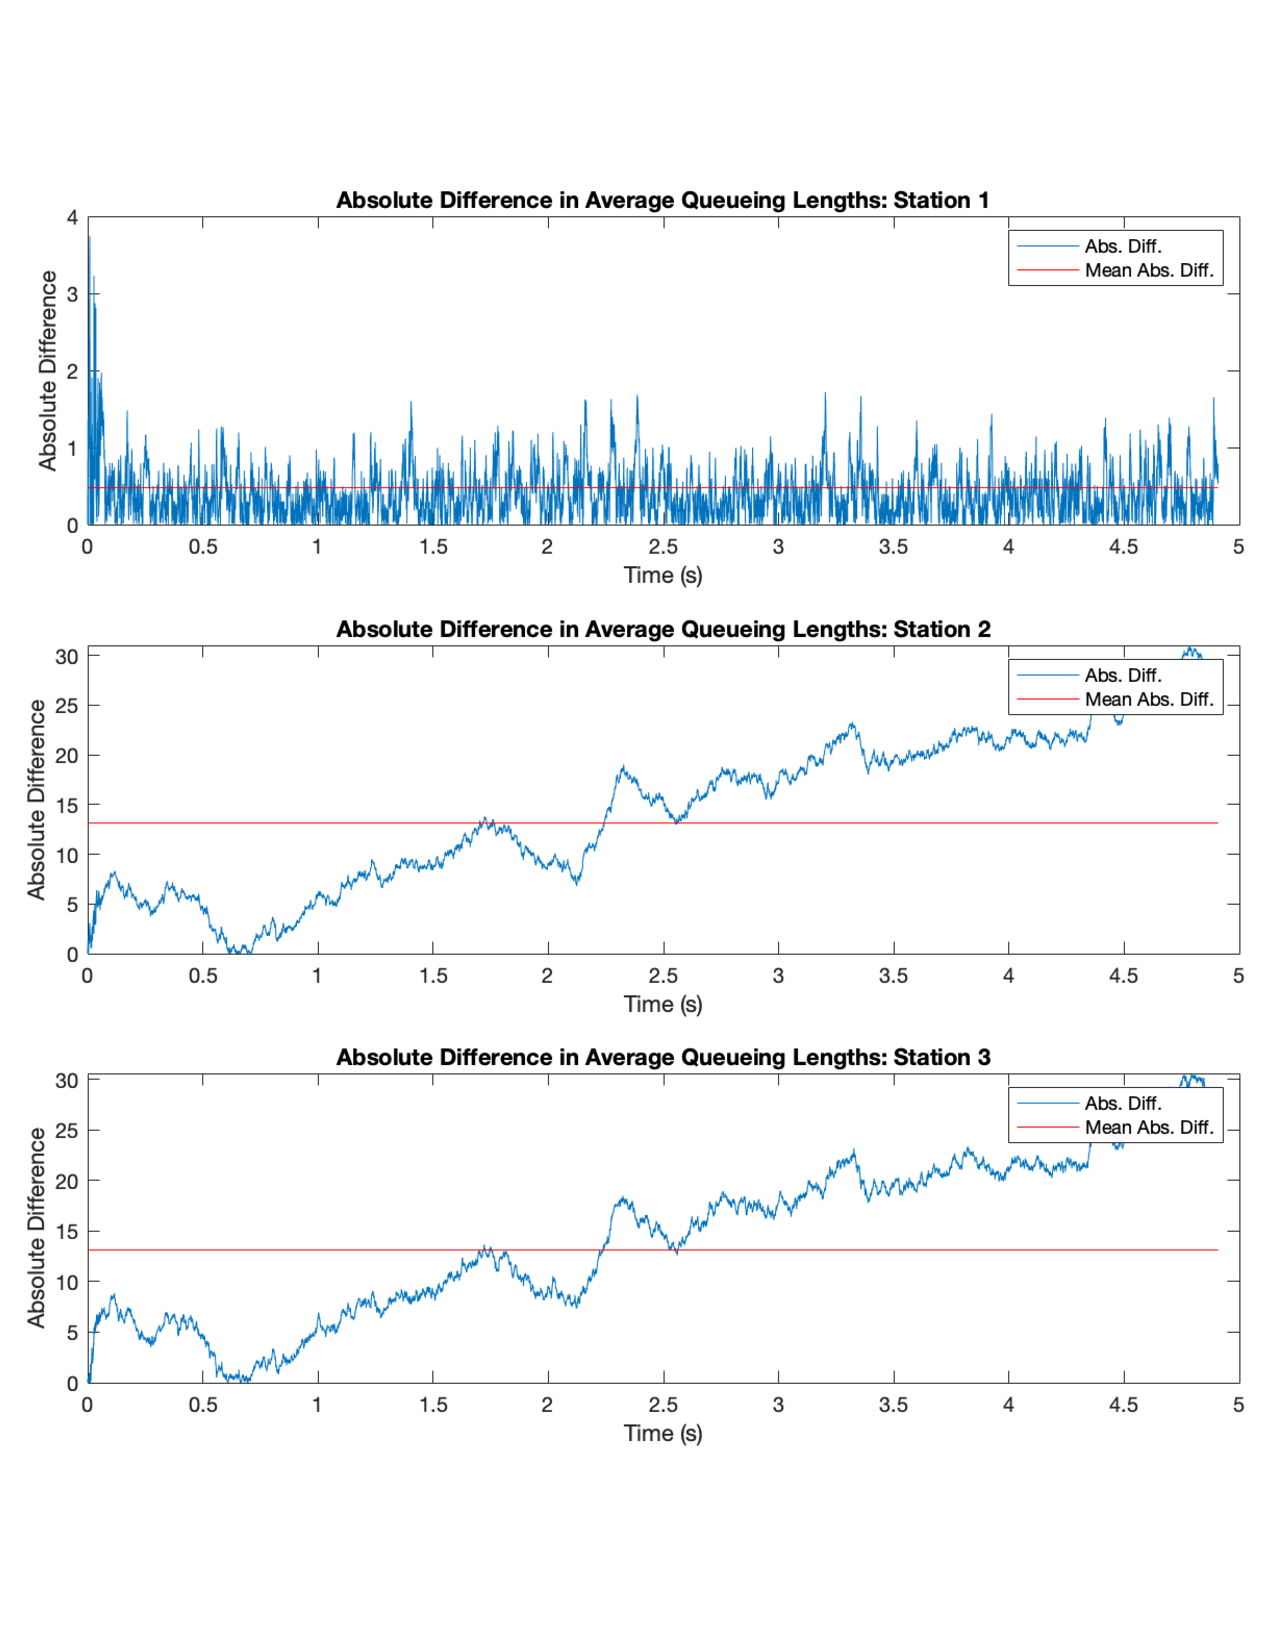
\includegraphics[width=100mm, scale=0.5]{abs_diff_bottleneck_2.pdf}
\caption{Absolute Difference in Average Queue Lengths without Bottleneck Ex. 2: $err = 15.4\%$}
\label{fig:bottleneck_ex_2}
\end{center}
\end{figure}

\textbf{Final Experiments and Evaluation of Changing Server Concurrency Values}: We did a similar experiment to test the accuracy of our predicted parameters for the 3-station model multiple other server concurrency values, as shown in Table \ref{tab:sc_acc}. We have that when station 2 and station 3 have the same server concurrency values and those values are small, the error value increases which infers that our prediction is worse for these values. This shows that the quality of our prediction depends on the server concurrency values that we choose, and perhaps if there are severe bottlenecks in the system then our predictions will be worse. This could be fixed by purposefully re-training the model using server concurrency values that initiate these kind of bottlenecks. We therefore have that our predicted parameters for the queueing network are of good quality for many choices of server concurrency values, as shown in Table \ref{tab:sc_acc}, however for a few choices of the concurrency values we get worse error values. 

\begin{table}[h!]
\begin{center}
\begin{tabular}{|c|c|}
\hline
\multicolumn{1}{|l|}{Server Concurrency Values} & \multicolumn{1}{l|}{Error Value} \\ \hline
(80,40,20) & 5.65\% \\ \hline
(60,40,10) & 5.55\% \\ \hline
(50, 20, 10) & 4.3\% \\ \hline
(50, 10, 5) & 5.13\% \\ \hline
(50, 8, 5) & 7.65\% \\ \hline
(50, 5, 3) & 4.75\% \\ \hline
(50, 5, 5) & 15.7\% \\ \hline
(50, 2, 2) & 15.4\% \\ \hline
\end{tabular}
\end{center}
\caption{How Do the Server Concurrency Values Change the Error}
\label{tab:sc_acc}
\end{table}

\section{Conclusion}

\subsection{Final Evaluation and Comparison of our Machine Learning Algorithms Applied to Stochastic Processes}

Within this paper we have described, analysed and evaluated various machine learning methodologies for parameter estimation on stochastic processes, including: expectation-maximisation algorithms, Markov-chain Monte Carlo methods, and recurrent neural network methodologies. Furthermore, we have implemented each method with varying degrees of success. Tables \ref{tab:comparison_models} and \ref{tab:comparison_models2} show a summary and comparison of each method that we implemented, where in Table \ref{tab:comparison_models} `SL' denotes self-loops and `S.S' denotes steady-state. \\

\begin{table}[h!]
\begin{tabular}{|l|l|l|}
\hline
\textbf{Comparison Analysis} & \textbf{Gibbs Sampling} & \textbf{RNN} \\ \hline
Type of ML & MCMC & Explainable ML \\ \hline
Input Data & S.S Average Queue Length & Transient Av. Q. Length \\ \hline
Output Data & Estimated Service Demands & Topology of QN \\ \hline
Successful Implementation? & Yes & Yes \\ \hline
Suitable? & Yes & Yes \\ \hline
Model Type & Product Form QN & Closed QN w.o. SL \\ \hline
Multi-class Analysis Possible? & Yes & No \\ \hline
Excessive Comp. Constraints? & Yes & Yes \\ \hline
\end{tabular}
\caption{Comparison of Models}
\label{tab:comparison_models}
\end{table}

\begin{table}[h!]
\begin{tabular}{|l|l|l|}
\hline
\textbf{Comparison Analysis} & \textbf{Naive EM algorithm} & \textbf{Improved EM algorithm} \\ \hline
Type of ML & EM & EM \\ \hline
Input Data & Inter-Arrival times & Inter-Arrival Times \\ \hline
Output Data & Predicted MAP & Predicted MAP \\ \hline
Successful Implementation? & No & Yes \\ \hline
Suitable? & No & Yes \\ \hline
Model Type & MAP & ER-CHMM MAP \\ \hline
Multi-class Analysis Possible? & No & No \\ \hline
Excessive Comp. Constraints? & Yes & No \\ \hline
\end{tabular}
\caption{Comparison of Models}
\label{tab:comparison_models2}
\end{table}

We have found that machine learning on stochastic processes could be a very suitable and valuable tool for queueing network parameter prediction in a number of real-life scenarios. We have applied all of our implemented models to a number of synthetic scenarios, and in each scenario we have achieved high quality results. We applied our EM algorithm to real-life data from web-services traffic and found favourable results, which shows that our EM algorithm can be effectively applied to real data with high quality. It was much harder to find real-life data for our other models, therefore we evaluated them using purely synthetic examples with high quality results. A glaring issue with our models is the computational constraints that are placed upon them. Using my at-home computer, which obviously is not ideal and great improvements can be made when using a more powerful computer, the 10-station synthetic predictions for the RNN methodology took 18 hours to compute. For each Gibbs sampling example with more that 2 stations the computation time was between $3$ - $10$ hours. The only algorithm that was computationally quite good was the ER-CHMM structured EM algorithm, where I could achieve results for even very complicated MAPs relatively quickly. Additionally, there were other issues that we ran into, such as our first attempt at implementing the EM algorithm. The naive implementation of the EM algorithm had a dreadful run-time and very flawed results that depended far too much on the initial guesses of the parameters. Therefore, even though for some examples we would eventually converge on the correct solution, for many examples our implementation would fall into a local optima and give us inferior results. Therefore, we abandoned this implementation in favour of implementing the ER-CHMM structured EM algorithm, which gave us very favourable results. We still kept the theory behind the naive implementation in this paper as it was an interesting stepping stone on the path to a high quality implementation of the algorithm. \\

In juxtaposition to this, our Gibbs sampling algorithm worked smoothly. We had a very detailed implementation from Casale and Wang [Cas16], which we managed to implement in a fairly straight-forward manner. Additionally, the results we achieved were very favourable and showed high quality predictions of the demands. The least amount of time was spent honing and improving the implementation for Gibbs sampling in this project. This is partly due to the high technical difficulty of creating the EM algorithms and the RNN methodology, therefore most of the focus of this project was on those algorithms. In the future it would be very beneficial to experiment with more prior distributions; look at different MCMC methods; detail the comparisons between techniques to calculate the normalizing constant; and try our Gibbs sampling algorithm on more complex and different examples. We thought we would be able to complete these additional aspects in this project, however it was not to be. It is satisfying to see that the results we did manage to get had a high accuracy however.  \\

Our implementation of the RNN methodology for parameter prediction also worked fairly smoothly, with promising results. When we looked at the 3-station and 5-station examples our results were very favourable and had high accuracy, with an error of below 7\% for each. The issues only arose when we looked at a 10-station example. This is because the queueing network we were trying to predict had a high level of complexity, therefore predicting the topology of the network was difficult. Additionally, we could see quite a severe bottleneck occurring which affected the quality of our results, which we did not foresee happening before we implemented the method. This would suggest that even though RNN networks are capable of predicting aspects of queueing networks, in real life they may struggle if the queueing network is of a much higher complexity than the ones we looked at. \\

In conclusion, I am happy with the results of our implementation. It was frustrating to see how long each experiment took to be completed and it was difficult to understand the nuances behind each method of predicting parameters for queueing networks. There is no doubt about it: this is a challenging topic of study. Nevertheless, this was a fascinating and highly engaging topic of research that hopefully in the future will become much more prevalent. With this in mind, we will now discuss the further work that I would contemplate completing in the future to add to the research that has been done in this paper.

\subsection{Further Work}

There is an abundance of extra work that could be completed in this research area. I was actually quite blown away by the potential avenues that we could take this work further. We will summarise the most fascinating areas of further work within the following bullet points: 

\begin{enumerate}
    \item For the EM algorithm, we could have looked in more detail at matching the auto-correlation of the predicted MAP and the input traces created from real-life data. If we were to look at the auto-correlation of the trace data for many thousands of lag points we would see that our predicted MAP struggles to match it for large lag points. This is because the predicted MAP auto-correlation evened out at around 500 lag points, however the auto-correlation from the real trace data keeps changing. Matching these values further would have required far too much complex work to be included in this paper, nevertheless it would have been a very interesting problem to study. 
    \item For the EM algorithm, we could have looked to improve its efficiency by reformulating the inherently serial classical EM algorithm to exploit modern, massively parallel hardware architectures. We could have made the serial algorithm that we implemented into an algorithm that worked in parallel, which would have made it much faster. The following reference explains it in more detail: [Hor18]. 
    \item For the EM algorithm, we could have implemented our algorithm in a way such that an analysis of multi-class traces were possible. To accomplish this, we would have had to alter our ER-CHMM structure slightly to take into consideration the multiple classes. We did not do this because even the single-class case was a very complex problem to solve. Additionally, the computational constraints would have been very large. If we were to couple this point with the parallel implementation then that would lead to a very fruitful area of research. 
    \item If computation constraints were not a consideration, it would have been very beneficial to apply my algorithms to much larger and more complex MAPs and queueing networks. This applies to all machine learning algorithms that have been implemented in this project. This paper focuses on the suitability, theory and implementation of machine learning algorithms to stochastic processes, therefore we focused on applying our algorithms to fairly simple examples to demonstrate these actions. Very large and complex queueing networks would have been extremely time consuming, and in the future if we were to have access to large amounts of GPUs and fast computers this would be a crucial area of research. 
    \item It would have been great to implement more MCMC methods and experiment with their accuracy. For example, it would have been interesting to actually implement the Metropolis Hastings algorithm and evaluate it within this project. The main reason this was not considered in this project is because Casale and Wang had limited success in implementing this algorithm for demand estimation [Cas16]. Therefore I was of the opinion that actually implementing it would have taken too much time for inadequate results. Implementing the Metropolis Hastings algorithm and tweaking the work done by Casale and Wang would have been very interesting however; it is definitely an area of research that has large potential in the future. Additionally, we could have explored the MCMC method called slice sampling [Per18]. Comparing the accuracy of all of these methods against each other would have been a satisfying area of research. I was more focused on choosing the algorithm to explore that gave the best results; hence my focus on the Gibbs sampling algorithm. In the future, if I were to have more time and a greater access to fast computation, this would be possible to achieve. 
    \item Within the MCMC methods it would have been fascinating to compare the time constraints and differences in accuracy between various methods of obtaining the normalizing constants. In this report we focused on the theory and implementation of the Taylor Expansion method, however many other methods exist such as ICMI and ICM methods. This comparison is present in the paper by Casale and Wang [Cas16], therefore if the reader is interested they can access it there. We did not do this because it is explained in their paper that the most accurate method is the TE method, therefore we decided to use that. Additionally, LINE has an automatic method for computing the normalizing constant already, therefore in our implementation we just used that. 
    \item For the RNN learning methodology, it would have been interesting to apply our learning methodology to much more complex queueing networks, such as mixed multi-class networks and layered queueing networks. We did not accomplish this goal as it is a very complex area of study with devilishly difficult calculations. Our report did not focus on layered queueing networks, but it would have been satisfying to try and apply our algorithms to these as well. 
    \item An attempt was made to create more complex neural network models for the aim of estimating queueing network parameters. We tried to use LSTM and GRU networks for the same computations as the RNN network. The complication in implementing this arose from the fact that our RNN methodology was an explainable machine learning technique, where we used the fluid approximations directly in the calculations of the changing weights. Normally, it is fairly easy to change an RNN into an LSTM or GRU network. It became too complicated for me to implement it in this case, as the change in equations and computations gave me very unfavourable results. In the future, given more time, it would be interesting to see how suitable an LSTM or GRU model would be for the same problem. I believe it would let us predict the parameters of more complicated networks more efficiently, as we would avoid vanishing and exploding gradients. This is a topic for another paper however, as we could have focused all of our energy on just this topic. 
    \item A fairly obvious area of further work would be to apply our Gibbs sampling and RNN algorithms to real data, much like we did for our EM algorithm. It was possible to apply real data to the EM algorithm as this data was readily available. The problem arose for the other algorithms as I could not find easy access to real data for the average queue lengths of systems. Additionally, for Gibbs sampling the synthetic examples were good enough as all we needed as an input were the steady state queue length averages. Therefore, any real-world data would likely be quite similar. For the RNN network we would have required real data for execution traces that consisted of transient averages of queue lengths at each station. To do this, we could have created our own web service and kept track of the traffic running through it. Alas, this would have taken up too much time and was not a glaring priority for me. This is definitely an area of research for the future however. 
    \item As seen from our RNN methodology, we are required to train a new model for each queueing network that we aim to predict the parameters of. We have a slight leeway where we can use the same model on networks that only have different initial populations of nodes and different server concurrency values. Now, obviously this is not ideal because each time we want to predict the parameters of a queueing network we need to re-train our model on the fluid dynamics of that particular network. A fascinating area of research could be to implement a neural network model that can predict the parameters of multiple different types of queueing network without having to re-train the model. To be able to do this, we would need an insane amount of data and execution traces. We would need to feed in hundreds of thousands of different models with labels defining what the parameters are of those models. Then, from the execution traces and the labels, the neural network could predict the labels for new models. Obviously, the amount of data required to train a model for this problem would be massive. This is why, at this moment, it is not possible for us to do this. In the future however this could be an interesting area of research. I am unsure how feasible it would be though. 
    \item I had the idea of creating a GUI application as an extension to the LINE toolbox in MATLAB that could use some of the algorithms explained in this project and show the results in a clear manner where the user just has to click a few buttons to generate traces and then sit and watch the magic occur. Alas, this was just a pipe dream, as the algorithms take too long to compute for a successful application, and the technical side of this project was time consuming and challenging which meant I could not implement this in time. 
\end{enumerate}

\subsection{Related Work}

In this section we will discuss some related work to this project which helps to enforce why this is a relevant and important area of research in regards to the wider world of computing. 

% Sources 

\begin{enumerate}
    \item \textbf{Modeling and controlling autonomous mobility-on-demand systems}: there has been significant research recently into the area of controlling autonomous mobility-on-demand systems by using a BCMP queueing network approach. This is fascinating, as it seems possible to relate the work we do in this paper with parameter inference on BCMP queueing networks related to the area of robotics. This is detailed further in [Igl19]. 
    \item \textbf{Program driven performance prediction}: there is a focus in this line of work for the derivation of performance predictions from the analysis of code. A real-world application is the software `PerfPlotter', which is a tool used for performance analyses of Java programs [Per16]. The type of analysis that it uses is probabilistic symbolic execution, which generates a probability distribution function over a performance metric such as response time. Hence, the result of the performance analysis is a quantitative model instead of predictive. There are other related approaches within the performance prediction area of research, such as black-box methods. Black-box methods are particularly relevant for variability-intensive systems [Val17], which relate the configuration settings in a software system with their performance impact [Sie15], [Sie12]. 
    \item \textbf{Program driven generation of performance models}: there is a focus on research into the area of the generation of software performance models such as layered queueing networks [Fra09] from a `class of distributed applications whose components communicate solely by remote procedure calls [Gar20]' [Hri95]. We have that Brosig et al. have derived a component-based performance model from Java EE platform applications [Bro11] [Bro09]. Additionally, Tarvo et al. have derived a way to extract discrete-event simulation models from `a class of multi-threaded programs covering task-oriented applications [Tar14]'. These are examples of using simulation models instead of analytical models for the task of predicting performance related phenomena from queueing networks.
    \item \textbf{Other techniques to measure service demands of queueing networks}: there are many other methods to derive predicted service demands of queueing networks that we have not delved into in this project. These include: non-linear optimization [Awa17], linear regression [Pac08], quadratic programming [Inc18], clustering regression [Cre10], independent component analysis [Sha08] and pattern matching [Cre14]. Within our project we focused on one method for service demand estimation, which was the MCMC method Gibbs sampling. It is interesting to see that service demand estimation is such an important research area within the topic of queueing networks. 
    \item \textbf{Bayesian inference prediction of the transient behaviour and busy period in queueing systems}: there has been research into using Bayesian inference techniques to find the behaviour of queueing systems using inter-arrival data instead of average queue lengths. [Sut11].
    \item \textbf{Identification and Analysis of Bottlenecks in Production Systems}: There is research into the area of how bottlenecks affect production systems [Wan05], [Kik16], [Buz17]. These delve into how the performance of production lines are limited by the presence of bottlenecks, which are not desirable in most productions networks as there is a large hold up at certain stations in the network. 
\end{enumerate}

\clearpage

\section{Bibliography}

\begin{enumerate}

\item Abadi, M. & Agarwal, A. (2015). TensorFlow: Large-scale machine learning on heterogeneous
systems. Software available from tensorflow.org. [Aba15].

\item Ahmad BA. & Khairatul K. & Farnaza A. (2017). An assessment of patient waiting and consultation time in a primary healthcare clinic. Malays Fam Physician. 2017;12(1):14-21. Published Apr 30. [Ahm17].

\item Ahmed Z. & Elmekkawy T. & Bates S. (2011). Developing an efficient scheduling template of a chemotherapy treatment unit: A case study. Australas Med J. 2011;4(10):575-588. doi:10.4066/AMJ.2011.837. [Ahm11]. 

\item Awad, M. & Menasce, D. (2017). Deriving Parameters for Open and Closed QN Models of Operational Systems Through Black Box Optimization. In ICPE. [Awa17]. 

\item Bahadori M. & Mohammadnejhad SM. & Ravangard R. & Teymourzadeh E. (2014). Using queuing theory and simulation model to optimize hospital pharmacy performance. Iran Red Crescent Med J. 2014;16(3):e16807. doi:10.5812/ircmj.16807. [Bah14].

\item Balsamo, S. Performance Evaluation: Origins and Directions. Product Form Queueing Networks. (2001). Part of the Lecture Notes in Computer Science book series (LNCS, volume 1769). [Bal01].

\item Bolch et. Al. (2006). Queueing Networks and Markov Chains : Modeling and Performance Evaluation with Computer Science Applications. John Wiley and Sons Publishing. Canada. [Bol06].

\item Bortolussi, L. & Hillston, J. & Latella, D. & MASSINK, M. (2013). Continuous approximation of collective system behaviour: A tutorial. Performance Evaluation 70, 5, 317–349. [Bor13]. 

\item Boucherie, J. et. Al. (2011). Queuing Networks: A Fundamental Approach. [Bou11].

\item Brazenas, M. (2019). Investigation of Phase-Type Distribution of Fourth Order Structures for Fitting and Markov Arrival Process Fitting by Expectation Maximization Algorithm Parallelization. Doctoral Dissertation, Kaunas, Kaunas University of Technology. [Bra19]. 

\item Brosig, F. & Huber, N. & Kounev, S. (2011). Automated Extraction of Architecture-level Performance Models of Distributed Component-based Systems. In ASE. [Bro11].

\item Brosig, F. & Kounev, S. & Krogmann, K. (2009). Automated extraction of Palladio component models from running enterprise Java applications. In VALUETOOLS. [Bro09].

\item Buchholz, P. (2003). An EM Algorithm for MAP Fitting from Real Traffic Data. Springer-Verlag. Berlin. [Buc03].

\item Buzen, J. (1971). Analysis of system bottlenecks using a queueing network model. 10.1145/800024.808355. [Buz71].

\item Buzen, J. & Denning, P. (1979). Measuring and Calculating Queue Length Distributions.
Department of Computer Science Technical Reports. Paper 246. https://docs.lib.purdue.edu/cstech/246. [Buz79].

\item Casale, G. et al. (2020). LINE User Manual. [Lin20]. 

\item Casale, G. Wang, W. & Sutton, C. (2016). A Bayesian Approach to Parameter Inference in Queueing Networks. ACM Trans. Model. Comput. Simul.,27(1). [Cas16].

\item Casale, G. & Wang, W. (2013) Bayesian Service Demand Estimation Using Gibbs Sampling. Proceedings of the 2012 IEEE 20th International Symposium on Modeling, Analysis  Simulation of Computer and Telecommunication Systems (MASCOTS). [Cas13]. 

\item Casale, G. & Zhang, E. & Smirn, E. (2010). KPC-Toolbox: Best Recipes for Automatic Trace Fitting Using Markovian Arrival Processes. Preprint submitted to Elsevier Science. [Cas10].

\item Chakravarthy, S. (2001). Markovian Arrival Processes. John Wiley and Sons Publishing. [Cha01]. 

\item Chollet, F., et al. Keras. https://keras.io, 2015. [Cho15]. 

\item Cohen, J. (1982). The Single Server Queue, Volume 8, 2nd Edition. North Holland. [Coh82]. 

\item Cremonesi, P. & Dhyani, K. & Sansottera, A. (2010). Service Time Estimation with a Refinement Enhanced Hybrid Clustering Algorithm. In International Conference on Analytical and Stochastic Modeling Techniques and Applications. Springer, pp. 291–305. (2010). [Cre10].

\item Cremonesi, P. & Sansoretta, A. (2014). Indirect Estimation of Service Demands in the Presence of Structural Changes. Performance Evaluation 73, 18–40. [Cre14].

\item Dragu, V. & Dinu, O. & Ruscă, A. & Burciu, Ş. & Roman, A. (2017). Queuing Theory Models used for Port Equipment Sizing. IOP Conference Series: Materials Science and Engineering, Volume 227, Issue 1, pp. 012040. [Dra17].

\item Franks, G. & Al-Omari, T. & Woodside, M. & Das, O. & Derisavi, S. (2009). Enhanced Modeling and Solution of Layered Queueing Networks. IEEE Trans. Software Eng. 35, 2, 148–161. [Fra09].

\item Garbi, G et al. (2020). Learning Queueing Networks by Recurrent Neural Networks. Accessible at: https://pdfs.semanticscholar.org/7f7c/12bcc23ba098ad5
a4a0ad251bd92e9b9c27a.pdf. [Gar20]. 

\item Geist, R. & Trivedi, K. (1982). Queueing Network Models in Computer System Design. Mathematics Magazine Vol. 55, No. 2, pp. 67-80 (14 pages)
Published By: Taylor & Francis, Ltd. [Gei82]. 

\item Gelenbe, E. & Pujolle, G. (1998). Introduction to Queueing Networks. 2nd Edition. [Gel98].

\item Gillespie, Daniel. (1991). Markov Processes, 1st Edition. Academic Press. [Gil91].

\item Harville D.A. (1997) Idempotent Matrices. In: Matrix Algebra From a Statistician’s Perspective. Springer, New York, NY. https://doi.org/10.1007/0-387-22677-X\_10. [Har97].

\item Horvath, G. et al. (2018). Parallel Algorithms for Fitting Markov Arrival Processes. Preprint Submitted to Elsevier. [Hor18]. 

\item Horvath, G. & Okamura, H. (2013). A Fast EM algorithm for Fitting Marked Markov Arrival Processes with a new Special Structure. [Hor13]. 

\item Horvath, G. Buchholz, P. & Telek, M. (2005). A MAP Fitting Approach with
Independent Approximation of the inter-arrival time distribution and the lag correlation. In Quantitative Evaluation of Systems, 2005. Second International Conference on the, pages 124–133. IEEE. [Hor05].

\item Hrischuk, C. & Rolia, J. & Woodside, C. (1995). Automatic Generation of a Software Performance Model
Using an Object-oriented Prototype. In MASCOTS. [Hri95].

\item Ibe, O. (2013). Markov Processes for Stochastic Modeling. 2nd Edition. Elsevier. [Ibe13].

\item Iglesias, R. et al. (2019). A BCMP network approach to modeling and controlling autonomous mobility-on-demand systems. The International Journal of Robotics Research, 38(2–3), pp. 357–374. [Igl19].

\item Incerto, E. & Napolitano, A. & Tribastone, M. (2018). Moving horizon estimation of service demands in queuing networks. In MASCOTS. [Inc18]. 

\item Internet Traffic Archive. Accessible at: http://beta.sigcomm.org/ITA. [ITA]. 

\item Kawase Y. & Kasahara S. (2017) Transaction-Confirmation Time for Bitcoin: A Queueing Analytical Approach to Blockchain Mechanism. In: Yue W., Li QL., Jin S., Ma Z. (eds) Queueing Theory and Network Applications. QTNA 2017. Lecture Notes in Computer Science, vol 10591. Springer, Cham. https://doi.org/10.1007/978-3-319-68520-5\_5. [Kaw17].

\item Kikolski, M. (2016). Identification of Production Bottlenecks with the use of Plant Simulation Software. ISMSME Volume 8 Issue 4. DOI: https://doi.org/1
0.1515/emj-2016-0038 | Published online: 27 Jan 2017. [Kik16]. 

\item King, T. (1984). Application of Queueing Theory to Communication Networks. HMSO London. [Kin84].

\item Kingma, P. & BA, J. (2015). Adam: A method for stochastic optimization. In 3rd International Conference on Learning Representations, ICLR 2015, San Diego, CA, USA, May 7-9, 2015, Conference Track Proceedings Y. Bengio and Y. LeCun, Eds. [Kin15]. 

\item Kleinrock, L. (1976). Queueing Systems: Theory, Volume 1. Wiley-interscience Publication. university of Michigan. [Kle76].

\item Kurtz, G. (1970). Solutions of Ordinary Differential Equations as Limits of Pure Markov Processes. In J. Appl. Prob. vol. 7, pp. 49–58. [Kur70]. 

\item Michaelides, M. & Hillston, J. & Sanguinetti, G. (2019). Geometric Fluid Approximation for General
Continuous-time Markov Chains. [Mic19]. 

\item Molnar, C. (2019). Interpretable machine learning. A Guide for Making Black Box Models Explainable. Available at: https://christophm.github.io/interpreta
ble-ml-book/.

\item Nguyen, V. (1993). Fluid and Diffusion Approximations of A Two-Station Mixed Queueing Network. Sloan School of Management, M.I.T., Cambridge, MA 02139. [Ngu93]. 

\item Nosek, RA. & Wilson, JP. (2001). Queuing theory and customer satisfaction, a review of terminology, trends, and applications to pharmacy practice. Hosp Pharm. 2001;36:275. [Nos01]. 

\item Okamura, H. et al. (2008). An EM algorithm for a Superposition of Markovian Arrival Processes. Department of Information Engineering, Graduate School of Engineering,
Hiroshima University, Japan. Accessible at: http://www.kurims.k
yoto-u.ac.jp/~kyodo/kokyuroku/contents/pdf/1589-28.pdf. [Oka08]. 

\item Pacifici, G. et al. (2008). CPU demand for web serving: Measurement analysis and dynamic estimation. Performance Evaluation 65, 6-7, 531–553. [Pac08]. 

\item Pardoux, É. (2008). Markov Processes and Applications: Algorithms, Genome and Finance. John Wiley and Sons Ltd. [Par08].

\item Perez, I. & Hodge, D. & Kypraios, T. (2018). Auxiliary variables for Bayesian inference in multi-class queueing networks. Stat Comput 28, 1187–1200. https://
doi.org/10.1007/s11222-017-9787-x. [Per18]. 

\item PerfPlotter Software. (2016). Accessible at: https://chenbihuan.github.io/perf
plotter/. [Per16].

\item Patel, B. & Bhathawala, P. (2012). Case Study for Bank ATM Queuing Model. International Journal of Engineering Research and Applications (IJERA) ISSN: 2248-9622 www.ijera.com Vol. 2, Issue 5, pp.1278-1284. [Pat12]. 

\item  Rachi, A. & Sadre, R. & Boudewijn, H. (2003). Fitting
world-wide web request traces with the EM-algorithm. Performance Evaluation,
52(2):175–191. [Rac03]. 

\item Saputro, D. et al. (2017). Prior and Posterior Dirichlet Distributions on Bayesian Networks. AIP conference proceedings 1827. [Sap17]. 

\item Schüssler, M. & Münker, T. & Nelles, O. (2019). Deep Recurrent Neural Networks for Nonlinear System Identification. IEEE Symposium Series on Computational Intelligence (SSCI), Xiamen, China, pp. 448-454, doi: 10.1109/SSCI44817.2019.9003133. [Sch19].

\item Sharma, A. & Bhagwan, R. & Choudhury, M. & Golubchik, L. & Govindan, R. & Voelker, G. (2008).
Automatic request categorization in internet services. ACM SIGMETRICS Performance Evaluation Review 36, 2, 16–25. [Sha08].

\item Shortle, J et. Al. (2018). Fundamentals of Queueing Theory. Chapter 3, Simple Markovian Queueing Models. Wiley Publishing. [Sho18].

\item Siegmund, N. & Grebhahn, A. & Apel, S. & Kastner, C. (2015). Performance-influence Models for Highly Configurable Systems. In ESEC/FSE. [Sie15].

\item Siegmund, N. & Kolesnikov, S. & Kastner, C. & Apel, S. & Batory, D. & Rosenmuller, M. &
Saake, G. (2012). Predicting performance via automated feature-interaction detection. In ICSE pp. 167–177. [Sie12]. 

\item Sutton, C. & Jordan, M. (2011). Bayesian Inference for Queueing Networks and Modeling of Internet Traffic Services. The Annals of Applied Statistics 2011, Vol. 5, No. 1, 254–282. [Sut11].

\item Tarvo, A. & Reiss, S. (2014). Automated Analysis of Multithreaded Programs for Performance Modeling. In ASE. [Tar14].

\item Telek, M. & Horvath, G. (2007). A Minimal Representation of Markov Arrival Processes and a Moments Matching Method. Performance Evaluation Elsevier Volume 64, Issues 9–12, Pages 1153-1168. [Tel07]. 

\item Tolver, Anders. (2016). An Introduction to Markov Chains. Lecture Notes, University of Copenhagen. Accessible at: http://web.math.ku.dk/noter/filer/s
toknoter.pdf. [Tol16].

\item Valov, P. & Petkovich, J. & Guo, J. & Fischmeister, S. & Czarnecki, K. (2017). Transferring Performance Prediction Models Across Different Hardware platforms. In ICPE. [Val17].

\item Wang, Y., Zhao, Q. & Zheng, D. Bottlenecks in production networks: An overview. J. Syst. Sci. Syst. Eng. 14, 347–363. https://doi.org/10.1007/s11518-006-0198-3. [Wan05].

\item Wong, X. Ahmed, S. Zulkift, F & Ramasamy, A. . (2009). An approach for analyzing queuing systems using Markov Chain Monte Carlo methods : A traffic flow case study. IEEE Student Conference on Research and Development (SCOReD), Serdang, 2009, pp. 41-44, doi: 10.1109/SCORED.2009.5443360. [Won09]. 

\item Xiao, H. and Zhang, G. (2010). The Queuing Theory Application in Bank Service Optimization. 2010 International Conference on Logistics Systems and Intelligent Management (ICLSIM), Harbin pp. 1097-1100, doi: 10.1109/ICLSIM.
2010.5461127. [Xia10].

\item Zhang, Y. & Qi, D. & Jiang, W. & Lei, S. (2016). Optimal Allocation of Changing Station for Electric Vehicle Based on Queuing Theory. PROMET - Traffic&Transportation. 28. 10.7307/ptt.v28i5.1974. [Zha16].

\item Zhu, L. & Casale, G. & Perez, I. (2020). Fluid Approximation of Closed Queueing Networks with Discriminatory Processor Sharing. Performance Evaluation. 139. 102094. 10.1016/j.peva.2020.102094. [Zhu20].




\end{enumerate}

\clearpage

\section{Appendix}

\subsection{Ethical Checklist}

\begin{table}[h!]
    \centering
    \begin{tabular}{|p{12.3cm}|l | l |}
    \hline
         & Yes & No 														  \\ \hline
        \cellcolor{green!20}\textbf{Section 1: HUMAN EMBRYOS/FOETUSES} &  &  		  \\ \hline
        Does your project involve Human Embryonic Stem Cells? &  & x 				  \\ \hline
        Does your project involve the use of human embryos? &  & x 					  \\ \hline
        Does your project involve the use of human foetal tissues / cells? &  & x 			  \\ \hline
        \cellcolor{green!20}\textbf{Section 2: HUMANS} &  & 						 	  \\ \hline
        Does your project involve human participants? &  & x 						  \\ \hline
        \cellcolor{green!20}\textbf{Section 3: HUMAN CELLS / TISSUES} &  &  			  \\ \hline
        Does your project involve human cells or tissues? (Other than from 
        "Human Embryos/Foetuses" i.e. Section 1)? &  & x 							  \\ \hline
        \cellcolor{green!20}\textbf{Section 4: PROTECTION OF PERSONAL DATA} &  &  	  \\ \hline
        Does your project involve personal data collection and/or processing? &  &  x		  \\ \hline
        Does it involve the collection and/or processing of sensitive personal data 
        (e.g. health, sexual lifestyle, ethnicity, political opinion, 
        religious or philosophical conviction)? &  & x 								  \\ \hline
        Does it involve processing of genetic information? &  & x 						  \\ \hline
        Does it involve tracking or observation of participants? 
        It should be noted that this issue is not limited to surveillance or localization data.
        It also applies to Wan data such as IP address, MACs, cookies etc. &  & x 		  \\ \hline
        Does your project involve further processing of previously collected personal data 
        (secondary use)? For example Does your project involve 
        merging existing data sets? &  & x									  \\ \hline
        \cellcolor{green!20}\textbf{Section 5: ANIMALS} &  &  						  \\ \hline
        Does your project involve animals? &  & x 									  \\ \hline
        \cellcolor{green!20}\textbf{Section 6: DEVELOPING COUNTRIES} &  &  			  \\ \hline
        Does your project involve developing countries? &  & x 						  \\ \hline
        If your project involves low and/or lower-middle income countries,
         are any benefit-sharing actions planned? &  & x 							  \\ \hline
        Could the situation in the country put the individuals taking part
         in the project at risk? &  & x 											  \\ \hline
        \cellcolor{green!20}\textbf{Section 7: ENVIRONMENTAL 
        PROTECTION AND SAFETY} &  &  										  \\ \hline
        Does your project involve the use of elements
         that may cause harm to the environment, animals or plants? &  & x 				  \\ \hline
        Does your project deal with endangered fauna and/or flora /protected areas? &  & x 	  \\ \hline
        Does your project involve the use of elements that may cause 
        harm to humans, including project staff? &  & x 								  \\ \hline
        Does your project involve other harmful materials or equipment, 
        e.g. high-powered laser systems? &  & x								 	  \\ \hline
        \end{tabular}
        \caption{Ethics Checklist, part 1. Adapted from the Imperial College Department of Computing website
        \url{https://www.doc.ic.ac.uk/lab/msc-projects/ethics-checklist.xlsx}.}
        \label{tab:ethical_checklist1}
        \end{table}
\begin{table}[h!]
    \centering
    \begin{tabular}{|p{12.3cm}|l | l |}
    \hline         
    & Yes & No 															  \\ \hline
        \cellcolor{green!20}\textbf{Section 8: DUAL USE} &  &  						  \\ \hline
        Does your project have the potential for military applications? &  & x 				  \\ \hline
        Does your project have an exclusive civilian application focus? &  & x 			  \\ \hline
        Will your project use or produce goods or information that will require 
        export licenses in accordance with legislation on dual use items? &  & x 			  \\ \hline
        Does your project affect current standards in military ethics ? e.g., 
        global ban on weapons of mass destruction, issues of
         proportionality, discrimination of combatants and accountability 
         in drone and autonomous robotics 
        developments, incendiary or laser weapons? &  & x 							  \\ \hline
        \cellcolor{green!20}\textbf{Section 9: MISUSE} &  &  							  \\ \hline
        Does your project have the potential for 
        malevolent/criminal/terrorist abuse? &  & x 								  \\ \hline
        Does your project involve information on/or the use of biological-,
        chemical-, nuclear/radiological-security sensitive materials and explosives, 
        and means of their delivery? &  & x 										  \\ \hline
        Does your project involve the development of technologies or the 
        creation of information that could have severe negative impacts on human 
        rights standards (e.g. privacy, stigmatization, discrimination), if misapplied? &  & x 	  \\ \hline
        Does your project have the potential for terrorist or criminal abuse e.g.
        infrastructural vulnerability studies, cybersecurity related project? &  & x 			  \\ \hline
        \cellcolor{green!20}\textbf{SECTION 10: LEGAL ISSUES} &  &  				  \\ \hline
        Will your project use or produce software for which there 
        are copyright licensing implications? &  & x 								  \\ \hline
        Will your project use or produce goods or information for 
        which there are data protection, or other legal implications? &  & x 				  \\ \hline
        \cellcolor{green!20}\textbf{SECTION 11: OTHER ETHICS ISSUES} &  &  			  \\ \hline
        Are there any other ethics issues that should be taken into consideration? &  & x 	  \\ \hline
    \end{tabular}
    \caption{Ethics Checklist, part 2. Adapted from the Imperial College Department of Computing website \url{https://www.doc.ic.ac.uk/lab/msc-projects/ethics-checklist.xlsx}.}
    \label{tab:ethical_checklist}
\end{table}
\end{document}
